% Options for packages loaded elsewhere
% Options for packages loaded elsewhere
\PassOptionsToPackage{unicode}{hyperref}
\PassOptionsToPackage{hyphens}{url}
\PassOptionsToPackage{dvipsnames,svgnames,x11names}{xcolor}
%
\documentclass[
  hebrew,
  letterpaper,
  DIV=11,
  numbers=noendperiod]{scrreprt}
\usepackage{xcolor}
\usepackage{amsmath,amssymb}
\setcounter{secnumdepth}{5}
\usepackage{iftex}
\ifPDFTeX
  \usepackage[T1]{fontenc}
  \usepackage[utf8]{inputenc}
  \usepackage{textcomp} % provide euro and other symbols
\else % if luatex or xetex
  \usepackage{unicode-math} % this also loads fontspec
  \defaultfontfeatures{Scale=MatchLowercase}
  \defaultfontfeatures[\rmfamily]{Ligatures=TeX,Scale=1}
\fi
\usepackage{lmodern}
\ifPDFTeX\else
  % xetex/luatex font selection
  \setmainfont[]{Arial}
  \setsansfont[]{Arial}
  \setmonofont[]{Courier New}
\fi
% Use upquote if available, for straight quotes in verbatim environments
\IfFileExists{upquote.sty}{\usepackage{upquote}}{}
\IfFileExists{microtype.sty}{% use microtype if available
  \usepackage[]{microtype}
  \UseMicrotypeSet[protrusion]{basicmath} % disable protrusion for tt fonts
}{}
\makeatletter
\@ifundefined{KOMAClassName}{% if non-KOMA class
  \IfFileExists{parskip.sty}{%
    \usepackage{parskip}
  }{% else
    \setlength{\parindent}{0pt}
    \setlength{\parskip}{6pt plus 2pt minus 1pt}}
}{% if KOMA class
  \KOMAoptions{parskip=half}}
\makeatother
% Make \paragraph and \subparagraph free-standing
\makeatletter
\ifx\paragraph\undefined\else
  \let\oldparagraph\paragraph
  \renewcommand{\paragraph}{
    \@ifstar
      \xxxParagraphStar
      \xxxParagraphNoStar
  }
  \newcommand{\xxxParagraphStar}[1]{\oldparagraph*{#1}\mbox{}}
  \newcommand{\xxxParagraphNoStar}[1]{\oldparagraph{#1}\mbox{}}
\fi
\ifx\subparagraph\undefined\else
  \let\oldsubparagraph\subparagraph
  \renewcommand{\subparagraph}{
    \@ifstar
      \xxxSubParagraphStar
      \xxxSubParagraphNoStar
  }
  \newcommand{\xxxSubParagraphStar}[1]{\oldsubparagraph*{#1}\mbox{}}
  \newcommand{\xxxSubParagraphNoStar}[1]{\oldsubparagraph{#1}\mbox{}}
\fi
\makeatother


\usepackage{longtable,booktabs,array}
\newcounter{none} % for unnumbered tables
\usepackage{calc} % for calculating minipage widths
% Correct order of tables after \paragraph or \subparagraph
\usepackage{etoolbox}
\makeatletter
\patchcmd\longtable{\par}{\if@noskipsec\mbox{}\fi\par}{}{}
\makeatother
% Allow footnotes in longtable head/foot
\IfFileExists{footnotehyper.sty}{\usepackage{footnotehyper}}{\usepackage{footnote}}
\makesavenoteenv{longtable}
\usepackage{graphicx}
\makeatletter
\newsavebox\pandoc@box
\newcommand*\pandocbounded[1]{% scales image to fit in text height/width
  \sbox\pandoc@box{#1}%
  \Gscale@div\@tempa{\textheight}{\dimexpr\ht\pandoc@box+\dp\pandoc@box\relax}%
  \Gscale@div\@tempb{\linewidth}{\wd\pandoc@box}%
  \ifdim\@tempb\p@<\@tempa\p@\let\@tempa\@tempb\fi% select the smaller of both
  \ifdim\@tempa\p@<\p@\scalebox{\@tempa}{\usebox\pandoc@box}%
  \else\usebox{\pandoc@box}%
  \fi%
}
% Set default figure placement to htbp
\def\fps@figure{htbp}
\makeatother



\ifLuaTeX
\usepackage[bidi=basic,shorthands=off,provide=*]{babel}
\else
\usepackage[bidi=default,shorthands=off,provide=*]{babel}
\fi
\ifPDFTeX
\else
\babelfont{rm}[]{Arial}
\fi
\ifLuaTeX
  \usepackage{selnolig} % disable illegal ligatures
\fi


\setlength{\emergencystretch}{3em} % prevent overfull lines

\providecommand{\tightlist}{%
  \setlength{\itemsep}{0pt}\setlength{\parskip}{0pt}}

\ifPDFTeX
  \TeXXeTstate=1
  \newcommand{\RL}[1]{\beginR #1\endR}
  \newcommand{\LR}[1]{\beginL #1\endL}
  \newenvironment{RTL}{\beginR}{\endR}
  \newenvironment{LTR}{\beginL}{\endL}
\fi
\ifluatex
  \newcommand{\RL}[1]{\bgroup\textdir TRT#1\egroup}
  \newcommand{\LR}[1]{\bgroup\textdir TLT#1\egroup}
  \newenvironment{RTL}{\textdir TRT\pardir TRT\bodydir TRT}{}
  \newenvironment{LTR}{\textdir TLT\pardir TLT\bodydir TLT}{}
\fi


 


\KOMAoption{captions}{tableheading}
\makeatletter
\@ifpackageloaded{bookmark}{}{\usepackage{bookmark}}
\makeatother
\makeatletter
\@ifpackageloaded{caption}{}{\usepackage{caption}}
\AtBeginDocument{%
\ifdefined\contentsname
  \renewcommand*\contentsname{תוכן עניינים}
\else
  \newcommand\contentsname{תוכן עניינים}
\fi
\ifdefined\listfigurename
  \renewcommand*\listfigurename{רשימת תרשימים}
\else
  \newcommand\listfigurename{רשימת תרשימים}
\fi
\ifdefined\listtablename
  \renewcommand*\listtablename{רשימת טבלאות}
\else
  \newcommand\listtablename{רשימת טבלאות}
\fi
\ifdefined\figurename
  \renewcommand*\figurename{תרשים}
\else
  \newcommand\figurename{תרשים}
\fi
\ifdefined\tablename
  \renewcommand*\tablename{טבלה}
\else
  \newcommand\tablename{טבלה}
\fi
}
\@ifpackageloaded{float}{}{\usepackage{float}}
\floatstyle{ruled}
\@ifundefined{c@chapter}{\newfloat{codelisting}{h}{lop}}{\newfloat{codelisting}{h}{lop}[chapter]}
\floatname{codelisting}{רישום}
\newcommand*\listoflistings{\listof{codelisting}{רשימת רישומים}}
\makeatother
\makeatletter
\makeatother
\makeatletter
\@ifpackageloaded{caption}{}{\usepackage{caption}}
\@ifpackageloaded{subcaption}{}{\usepackage{subcaption}}
\makeatother
\usepackage{bookmark}
\IfFileExists{xurl.sty}{\usepackage{xurl}}{} % add URL line breaks if available
\urlstyle{same}
\hypersetup{
  pdftitle={תורת החומרים},
  pdfauthor={Alex Lugovskoy},
  pdflang={he},
  colorlinks=true,
  linkcolor={blue},
  filecolor={Maroon},
  citecolor={Blue},
  urlcolor={Blue},
  pdfcreator={LaTeX via pandoc}}


\title{תורת החומרים}
\author{Alex Lugovskoy}
\date{}
\begin{document}
\maketitle

\renewcommand*\contentsname{תוכן עניינים}
{
\setcounter{tocdepth}{2}
\tableofcontents
}

\bookmarksetup{startatroot}

\chapter{תורת
החומרים}\label{ux5eaux5d5ux5e8ux5ea-ux5d4ux5d7ux5d5ux5deux5e8ux5d9ux5dd}

קורס לסטודנטים של מסלול החומרים

אלכס לוגובסקוי 2026

\bookmarksetup{startatroot}

\chapter{}\label{section}

לכל העובדות שבמסירות נפשן הפריעו להופעת הספר

\bookmarksetup{startatroot}

\chapter{}\label{section-1}

\bookmarksetup{startatroot}

\chapter{פרק 1 --- אטומים, גרעינים ותגובות
גרעיניות}\label{ux5e4ux5e8ux5e7-1-ux5d0ux5d8ux5d5ux5deux5d9ux5dd-ux5d2ux5e8ux5e2ux5d9ux5e0ux5d9ux5dd-ux5d5ux5eaux5d2ux5d5ux5d1ux5d5ux5ea-ux5d2ux5e8ux5e2ux5d9ux5e0ux5d9ux5d5ux5ea}

\section{1.1 על מה הקורס
הזה?}\label{ux5e2ux5dc-ux5deux5d4-ux5d4ux5e7ux5d5ux5e8ux5e1-ux5d4ux5d6ux5d4}

לפני שנצלול לחומר, שאלה פשוטה: מה זה בכלל ``מדע החומרים''?

בשנה הראשונה vתחלתם ללמוד כימיה, פיזיקה ומתמטיקה, שהם הכלים הבסיסיים
שלנו. בקורס הזה נתחיל להשתמש בכלים האלה כדי להבין \emph{למה} חומרים
מתנהגים כמו שהם מתנהגים. למה ברזל קשה וזהב רך? למה זכוכית שקופה
ואלומיניום לא? למה קרמיקה מתנפצת בעוד מתכת מתעקלת? אלו שאלות של מדע
החומרים.

הפרק הראשון מתחיל מהרמה הכי בסיסית: האטום. לא כי זו מסורת אקדמית, אלא כי
תכונות של חומרים --- קשיות, הולכה חשמלית, חוזק, צבע --- כולן בסופו של
דבר נובעות מהאופן שבו אטומים בנויים ומהאופן שבו הם קשורים זה לזה. \#\#
1.2 מה אנחנו יודעים על אטום?

נראה כאילו אטומים הם דבר מוכר. לומדים עליהם עוד מבית ספר, שומעים וקוראים
כמעט בכל מקום, ובכל זאת --- מה באמת אנחנו יודעים עליהם?

\textbf{מה שכן ידוע:}

\begin{itemize}
\tightlist
\item
  לאטום יש \textbf{מסה} --- החל מ-1 יחידת מסה אטומית (`amu 'atomic mass
  unit או u פשוט 'unit') אצל מימן ועד 238 u אצל אורניום
\item
  המטען החשמלי הכולל של אטום הוא אפס, אך אטומים יכולים לאבד או לקבל
  אלקטרונים ולהפוך ל\textbf{יונים} שאלה כבר טעונים חשמלית.
\item
  לאטומים יש תכונות מגנטיות
\item
  לאטומים יש \textbf{גודל} ו\textbf{צורה} --- אם כי שני הדברים הללו
  מסובכים יותר מהצפוי.
\end{itemize}

\textbf{מה שלא שייך לאטום בודד:} צבע, ריח, מצב צבירה --- אלו תכונות של
\emph{אוסף} אטומים, לא של אטום בודד. אין לאטום בודד ``צבע'' או ``ריח'',
בדיוק כשם שאין לאדם בודד ``קהילה''. \#\# 1.3 בעיית הגודל האטומי

\subsection{הבעיה}\label{ux5d4ux5d1ux5e2ux5d9ux5d4}

נסו לחפש את ``הקוטר של אטום חמצן'' בשלושה ספרי עיון שונים:

{\def\LTcaptype{none} % do not increment counter
\begin{longtable}[]{@{}
  >{\raggedright\arraybackslash}p{(\linewidth - 2\tabcolsep) * \real{0.8026}}
  >{\raggedright\arraybackslash}p{(\linewidth - 2\tabcolsep) * \real{0.1974}}@{}}
\toprule\noalign{}
\begin{minipage}[b]{\linewidth}\raggedright
מקור
\end{minipage} & \begin{minipage}[b]{\linewidth}\raggedright
קוטר (Å)
\end{minipage} \\
\midrule\noalign{}
\endhead
\bottomrule\noalign{}
\endlastfoot
Periodic Chart of the Atoms (1979), Sargent-Welch & \(1.30 \pm 0.01\) \\
Chemical Bond Approach Project (1964), McGraw-Hill &
\(0.66 \pm 0.01\) \\
Handbook of Chemistry and Physics, 65th Ed. (1984), CRC Press &
\(1.40 \pm 0.01\) \\
\end{longtable}
}

שלושה מקורות מוסמכים, שלושה ערכים שונים. הטעויות בתוך כל מקור קטנות מאוד
--- פחות מאחוז. אז מי טועה?

\textbf{אף אחד לא.}

\subsection{למה שלושה ערכים
שונים?}\label{ux5dcux5deux5d4-ux5e9ux5dcux5d5ux5e9ux5d4-ux5e2ux5e8ux5dbux5d9ux5dd-ux5e9ux5d5ux5e0ux5d9ux5dd}

אטום אינו כדור קשיח עם גבול חד. מה שמסתתר תחת המילה ``גודל אטומי'' הוא
בעצם שאלה: \emph{איך מודדים?}
\pandocbounded{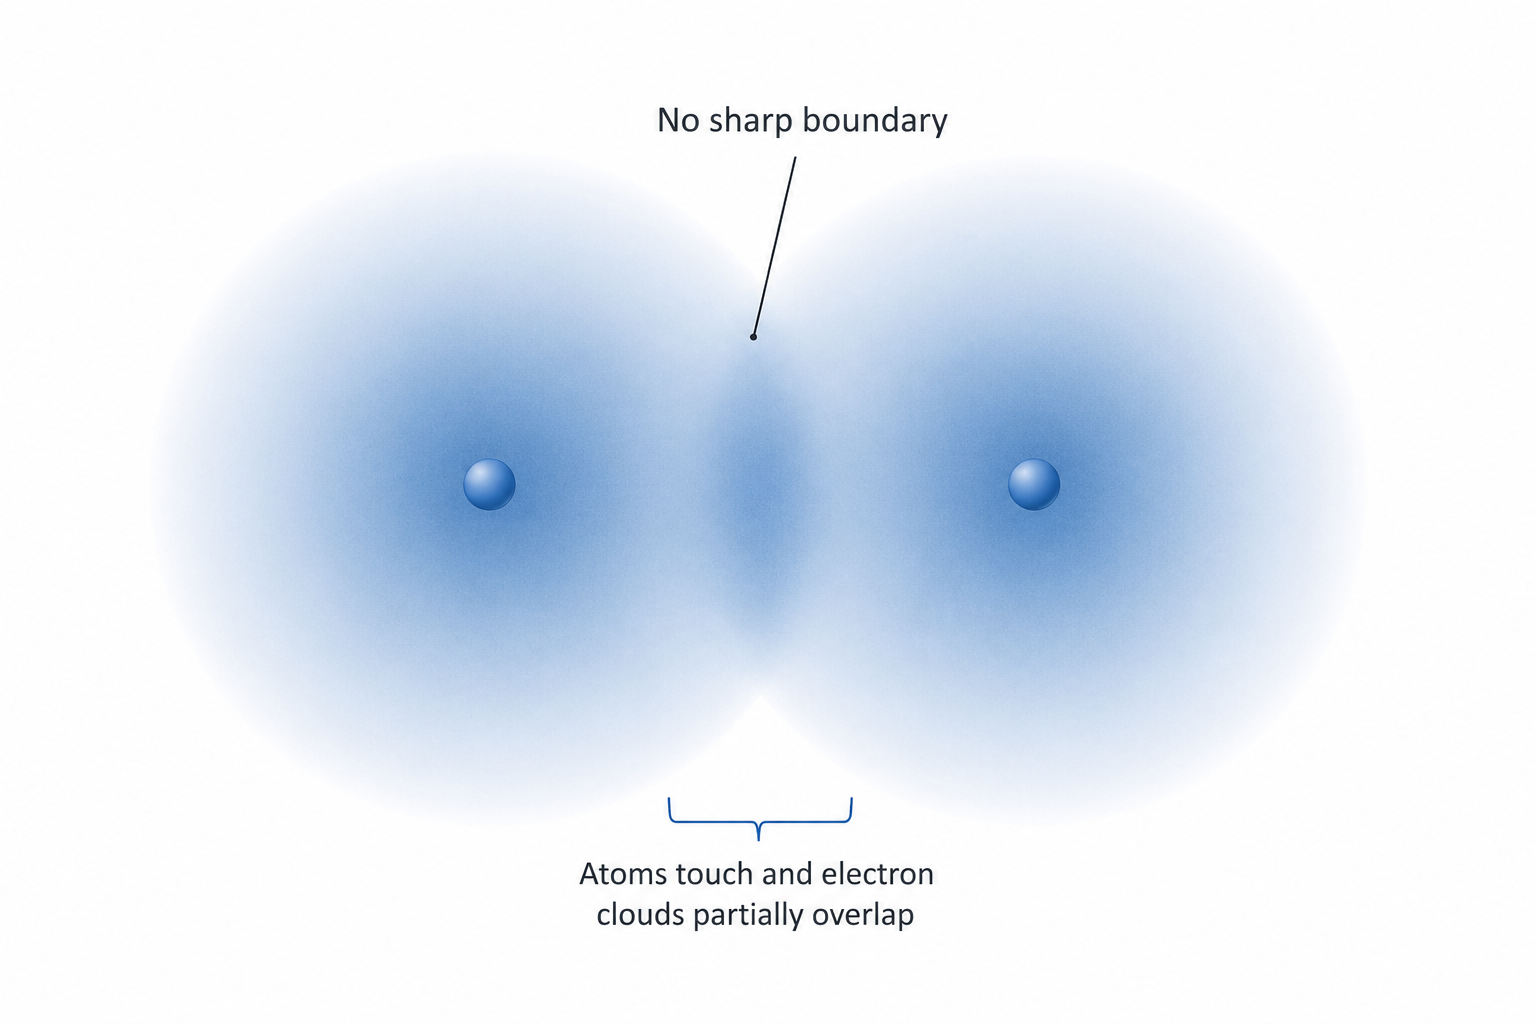
\includegraphics[keepaspectratio]{chapters/../images/image1.interatomicBorder.PNG}}

\begin{itemize}
\tightlist
\item
  \textbf{רדיוס קוולנטי} (covalent radius): מודדים את המרחק בין שני
  אטומי חמצן במולקולת \(\text{O}_2\) ומחלקים לשניים. זה הגודל של האטום
  כשהוא יוצר קשר כימי. מקבלים כ-0.66 Å.
\item
  \textbf{רדיוס ון-דר-ולס} (van der Waals radius): מודדים את המרחק
  המינימלי בין אטומי חמצן של מולקולות \emph{שונות} בגביש --- כלומר,
  כשאין ביניהם קשר כימי. מקבלים כ-1.40 Å.
\item
  שיטות ספקטרוסקופיות נותנות ערכים שלישיים.
\end{itemize}

כל אחד מהערכים נכון --- לשאלה שלה הוא עונה. לכן, בכל פעם שפוגשים ``רדיוס
אטומי'', חשוב לשאול: \textbf{איזה רדיוס? הנמדד באיזו שיטה? לאיזו מטרה?}

\subsection{צורת
האטום}\label{ux5e6ux5d5ux5e8ux5ea-ux5d4ux5d0ux5d8ux5d5ux5dd}

האינטואיציה אומרת ``כדור''. בפועל --- זוהי \textbf{הנחת עבודה} שימושית
מאוד, לא עובדה מדודה. צורת ענן האלקטרונים סביב הגרעין תלויה בסביבה: אטום
בוואקום שונה מאותו אטום בתוך גביש. בכל פעם שנניח ש''אטום = כדור'', זה
יהיה מודל --- ומודלים הם כלים, לא אמת מוחלטת.

מסר זה --- שמודלים הם כלים שימושיים אך מוגבלים --- יחזור שוב ושוב לאורך
כל הקורס (וגם מעבר לו). \#\# 1.4 מבנה הגרעין

\subsection{מה בתוך
האטום?}\label{ux5deux5d4-ux5d1ux5eaux5d5ux5da-ux5d4ux5d0ux5d8ux5d5ux5dd}

ניסויי ראת'רפורד (בתחילת המאה ה-20) הוכיחו שהאטום אינו ``בלתי ניתן
לחלוקה''. הוא מורכב מ:

\begin{itemize}
\tightlist
\item
  \textbf{גרעין} (nucleus) --- קטן מאוד, צפוף מאוד, טעון חיובית.
\item
  \textbf{אלקטרונים} (electrons) --- מקיפים את הגרעין, טעונים שלילית.
\end{itemize}

הגרעין עצמו מורכב מ\textbf{פרוטונים} (protons, מטען חיובי)
ו\textbf{נייטרונים} (neutrons, ללא מטען). שניהם נקראים יחד
\textbf{נוקלאונים} (nucleons).

\subsection{גודל הגרעין --- בעיית הריק
הגדול}\label{ux5d2ux5d5ux5d3ux5dc-ux5d4ux5d2ux5e8ux5e2ux5d9ux5df-ux5d1ux5e2ux5d9ux5d9ux5ea-ux5d4ux5e8ux5d9ux5e7-ux5d4ux5d2ux5d3ux5d5ux5dc}

רדיוס הגרעין מוערך לפי:

\begin{verbatim}
    $$R \approx 1.3 \times 10^{-15} \cdot Z^{1/3} \quad [\text{m}],$$
\end{verbatim}

כאשר Z הינו מטען הגרעין. רדיוס האטום כולו הוא כ-\(10^{-10}\) מ', ורדיוס
הגרעין כ-\(10^{-15}\) מ'. הגרעין קטן מהאטום \textbf{פי 100,000}. אם
מגדילים את הגרעין לגודל כדור כדורגל, האטום כולו יהיה בקוטר של 22 ק''מ.
רוב האטום הוא חלל ריק.

\subsection{מה מחזיק את הגרעין
ביחד?}\label{ux5deux5d4-ux5deux5d7ux5d6ux5d9ux5e7-ux5d0ux5ea-ux5d4ux5d2ux5e8ux5e2ux5d9ux5df-ux5d1ux5d9ux5d7ux5d3}

כל הפרוטונים בגרעין טעונים חיובית ודוחים זה את זה. מה מחזיק אותם?
\textbf{האינטראקציה הגרעינית החזקה} (strong nuclear force) --- כוח שלישי
לגמרי, שאינו חשמלי ואינו גרביטציוני. הוא פועל רק בין נוקלאונים ורק
במרחקים של \(\sim 10^{-15}\) מ'. בתחום זה הוא חזק בהרבה מהדחייה החשמלית;
מחוצה לו --- הוא פשוט לא קיים.

\subsection{סימון
גרעינים}\label{ux5e1ux5d9ux5deux5d5ux5df-ux5d2ux5e8ux5e2ux5d9ux5e0ux5d9ux5dd}

\[^A_Z X\]

\begin{itemize}
\tightlist
\item
  \(Z\) --- \textbf{מספר אטומי}: מספר הפרוטונים (קובע איזה יסוד זה)
\item
  \(A\) --- \textbf{מספר מסתי}: מספר הנוקלאונים הכולל
\end{itemize}

דוגמה: \(^{56}_{26}\text{Fe}\) --- ברזל עם 26 פרוטונים ו-30 נייטרונים.

\textbf{איזוטופים} --- אטומים של אותו יסוד עם מספר נייטרונים שונה.
פחמן-12 (\(^{12}_6\text{C}\)) יציב; פחמן-14 (\(^{14}_6\text{C}\))
רדיואקטיבי --- שניהם פחמן. \#\# 1.5 יציבות גרעינית וזמן מחצית חיים

{\def\LTcaptype{none} % do not increment counter
\begin{longtable}[]{@{}lll@{}}
\toprule\noalign{}
סוג גרעין & \(t_{1/2}\) & משמעות מעשית \\
\midrule\noalign{}
\endhead
\bottomrule\noalign{}
\endlastfoot
\textbf{יציב} & \(> 10^{18}\) שנה & לא נצפתה התפרקות מעולם \\
\textbf{רדיואקטיבי} & שניות עד מיליארדי שנים & ההתפרקות נמדדת ניסויית \\
\textbf{לא יציב} & שברי שניות & מתפרק כמעט מיידית \\
\end{longtable}
}

\(t_{1/2}\) מתאר \textbf{אוסף} אטומים סטטיסטית:

\[N(t) = N_0 \cdot \left(\frac{1}{2}\right)^{t/t_{1/2}}\]

\begin{quote}
\textbf{שאלה:} פחמן-14 עם \(t_{1/2} \approx 5730\) שנה --- בשברי עץ עתיק
נשאר \(\frac{1}{8}\) מהכמות המקורית. מתי נכרת העץ?
\end{quote}

גרעינים יציבים נמצאים ב''עמק היציבות'': \(\frac{Z^2}{A} < 46\) ויחס
פרוטונים-נייטרונים קרוב ל-1.
\pandocbounded{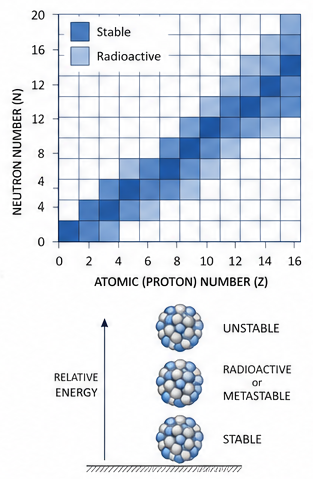
\includegraphics[keepaspectratio]{chapters/../images/image2.nucleusStability.png}}
\#\# 1.6 סוגי דעיכה רדיואקטיבית

{\def\LTcaptype{none} % do not increment counter
\begin{longtable}[]{@{}lll@{}}
\toprule\noalign{}
סוג & מה נפלט & הערה \\
\midrule\noalign{}
\endhead
\bottomrule\noalign{}
\endlastfoot
דעיכת \(\alpha\) & \(^4_2\text{He}\) & גרעין מאבד 2p + 2n \\
דעיכת \(\beta^-\) & \(e^-\) & נייטרון הופך לפרוטון \\
דעיכת \(\beta^+\) & \(e^+\) & פרוטון הופך לנייטרון \\
דעיכת \(\gamma\) & פוטון & אין שינוי בהרכב הגרעין \\
ביקוע ספונטני & שני גרעינים & הגרעין מתפצל \\
\end{longtable}
}

\pandocbounded{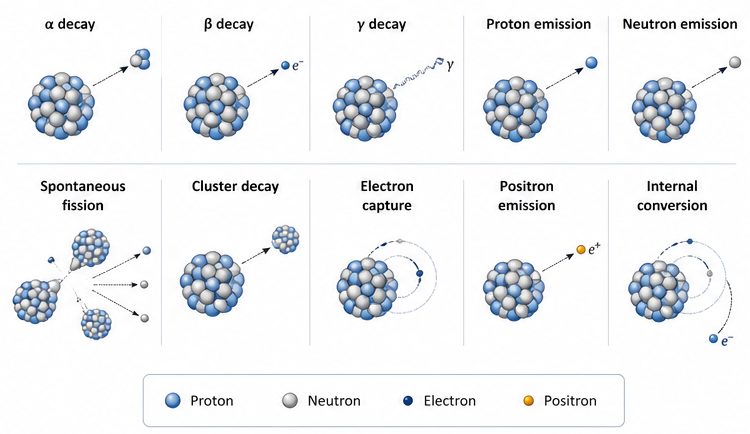
\includegraphics[keepaspectratio]{chapters/../images/image3.RadioactiveDecayTypes.png}}
אורניום-238 עובר 14 שלבי דעיכה עד להגעה לעופרת-206 היציבה.
\pandocbounded{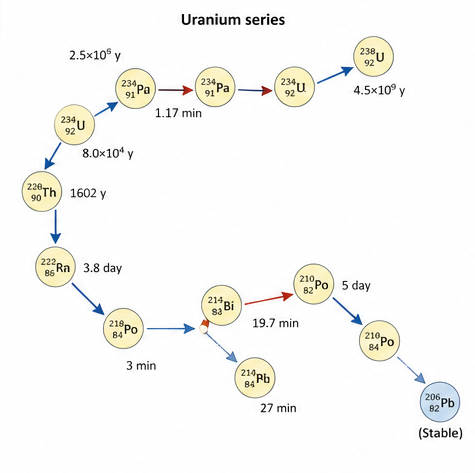
\includegraphics[keepaspectratio]{chapters/../images/image4.radioactiveSeries.png}}
\#\# 1.7 תגובות גרעיניות

\subsection{ראת'רפורד (1919) --- הסינתזה הגרעינית
הראשונה}\label{ux5e8ux5d0ux5eaux5e8ux5e4ux5d5ux5e8ux5d3-1919-ux5d4ux5e1ux5d9ux5e0ux5eaux5d6ux5d4-ux5d4ux5d2ux5e8ux5e2ux5d9ux5e0ux5d9ux5ea-ux5d4ux5e8ux5d0ux5e9ux5d5ux5e0ux5d4}

\[^{14}_7\text{N} + ^4_2\text{He} ;\to; ^{17}_8\text{O} + ^1_1\text{H}\]

הפעם הראשונה בהיסטוריה שאדם יצר יסוד חדש מיסוד אחר. בכימיה רגילה יסודות
אינם משתנים; בתגובה גרעינית --- \textbf{היסוד עצמו משתנה}.

שימור: מטען \(7+2=8+1\) ✓; מספר מסי \(14+4=17+1\) ✓

\subsection{פגם המסה --- מאיפה מגיעה האנרגיה
הגרעינית?}\label{ux5e4ux5d2ux5dd-ux5d4ux5deux5e1ux5d4-ux5deux5d0ux5d9ux5e4ux5d4-ux5deux5d2ux5d9ux5e2ux5d4-ux5d4ux5d0ux5e0ux5e8ux5d2ux5d9ux5d4-ux5d4ux5d2ux5e8ux5e2ux5d9ux5e0ux5d9ux5ea}

כל מהנדס כימי מכיר את שימור המסה. אבל בדיקת גרעינים חושפת סתירה לכאורה:
מסת הגרעין הנמדדת \textbf{קטנה} מסכום מסות הנוקלאונים הבודדים.

עבור סידן (20p + 20n):

\[\Delta m = m_\text{calc} - m_\text{observed} > 0\]

זהו \textbf{פגם המסה} (mass defect). לפי \(E = mc^2\), פגם המסה מייצג את
\textbf{אנרגיית הקישור הגרעינית} --- האנרגיה שהושקעה בבניית הגרעין.
כשגרעין נבנה, אנרגיה זו משתחררת. כשגרעין מתפצל (ביקוע) או כשגרעינים
מתאחדים (היתוך), ההפרש בין פגמי המסה של מגיבים לתוצרים יוצא כאנרגיה. זה
מקור עוצמתן האדירה של התגובות הגרעיניות --- לא ``דלק'' מיוחד, אלא המרת
מסה לאנרגיה.

\subsection{ביקוע
גרעיני}\label{ux5d1ux5d9ux5e7ux5d5ux5e2-ux5d2ux5e8ux5e2ux5d9ux5e0ux5d9}

\[^{235}_{92}\text{U} + ^1_0\text{n} ;\to; ^{137}_{56}\text{Ba} + ^{85}_{36}\text{Kr} + 17\cdot^1_0\text{n} + \Delta E\]

כל גרעין מניב 17 נייטרונים --- \textbf{תגובת שרשרת}. כ-80 שלבים מספיקים
לביקוע כל קילוגרם האורניום, תוך פחות \(10^{-6}\) שנייה.

\textbf{כור גרעיני לעומת פצצה:} ההבדל הוא בשליטה. שלוש דרכים לשלוט:
מתינים (מעכבים נייטרונים), מוטות בקרה (סופגים נייטרונים), עיצוב גיאומטרי
(מאפשרים לנייטרונים ``לברוח'' ללא פגיעה הגורמת להמשך תגובת שרשרת).
האנרגיה מחממת מים → קיטור → טורבינה --- בדיוק כמו תחנת כוח רגילה.

\subsection{היתוך
גרעיני}\label{ux5d4ux5d9ux5eaux5d5ux5da-ux5d2ux5e8ux5e2ux5d9ux5e0ux5d9}

\[^2_1\text{H} + ^3_1\text{H} ;\to; ^4_2\text{He} + ^1_0\text{n} + 17.6;\text{MeV}\]

{\def\LTcaptype{none} % do not increment counter
\begin{longtable}[]{@{}ll@{}}
\toprule\noalign{}
מקור אנרגיה & אנרגיה (kJ/mol) \\
\midrule\noalign{}
\endhead
\bottomrule\noalign{}
\endlastfoot
שריפת מתאן & 890 \\
ביקוע אורניום & \textasciitilde200,000 \\
היתוך D-T & \textasciitilde1,700,000 \\
\end{longtable}
}

ההסבר: פגם המסה של \(^4\text{He}\) גדול יותר מסכום פגמי המסה של
\(^2\text{H}\) ו-\(^3\text{H}\) --- ההפרש יוצא כאנרגיה.

\textbf{פצצת מימן:} ביקוע גרעיני משמש כ''מצת'' להצתת ההיתוך --- כי הגעה
לטמפרטורות של מאות מיליוני מעלות ניתן לעשות רק בפיצוץ גרעיני.

\textbf{היתוך מבוקר (ITER):} דאוטריום ממי ים, ללא פסולת רדיואקטיבית
ארוכת-חיים, ללא סכנת תגובת שרשרת. הבעיה: שמירת פלסמה ב-\(10^8\) מעלות
באמצעות כלואה מגנטית. הפרויקט טרם הגיע לפריצת הדרך. \#\# סיכום

שלושה מסרים עקרוניים מהפרק הזה:

\textbf{ראשית} --- מודלים הם כלים, לא מציאות. ``רדיוס אטומי'', ``כדור
קשיח'' --- כל מושג מוגדר לפי הצורך. יש לדעת מה מאחוריו.

\textbf{שנית} --- \(E = mc^2\) אינה רק נוסחה יפה. פגם המסה הוא דוגמה
קונקרטית: שימור המסה לבדו אינו מספיק --- יש לשמר את מסה+אנרגיה יחד.

\textbf{שלישית} --- סדרי גודל חשובים. גרעין קטן מאטום פי \(10^5\). היתוך
חזק משריפה פי \(10^3\).

\bookmarksetup{startatroot}

\chapter{פרק 2 --- מודל הקוונטים: ממשבר לפריצת
דרך}\label{ux5e4ux5e8ux5e7-2-ux5deux5d5ux5d3ux5dc-ux5d4ux5e7ux5d5ux5d5ux5e0ux5d8ux5d9ux5dd-ux5deux5deux5e9ux5d1ux5e8-ux5dcux5e4ux5e8ux5d9ux5e6ux5ea-ux5d3ux5e8ux5da}

\section{מבוא: מדוע הפיזיקה הקלאסית
נכשלה?}\label{ux5deux5d1ux5d5ux5d0-ux5deux5d3ux5d5ux5e2-ux5d4ux5e4ux5d9ux5d6ux5d9ux5e7ux5d4-ux5d4ux5e7ux5dcux5d0ux5e1ux5d9ux5ea-ux5e0ux5dbux5e9ux5dcux5d4}

בסוף המאה ה-19, פיזיקאים היו בטוחים שהם מבינים את העולם. ניוטון, מקסוול,
תרמודינמיקה --- הכל עבד מצוין. נותר, כך נדמה, רק למלא פרטים קטנים.

ואז הגיעו שלוש תוצאות ניסיוניות שלא ניתן היה להסביר. לא ``קשה להסביר''
--- \textbf{בלתי אפשרי} להסביר, עם כל כלי הפיזיקה הקלאסית. הן דרשו מהפכה
מחשבתית שלמה. \#\# 2.1 גלים אלקטרומגנטיים --- הבסיס

לפני שנבין מה השתבש, כמה מושגי יסוד על אור.
\pandocbounded{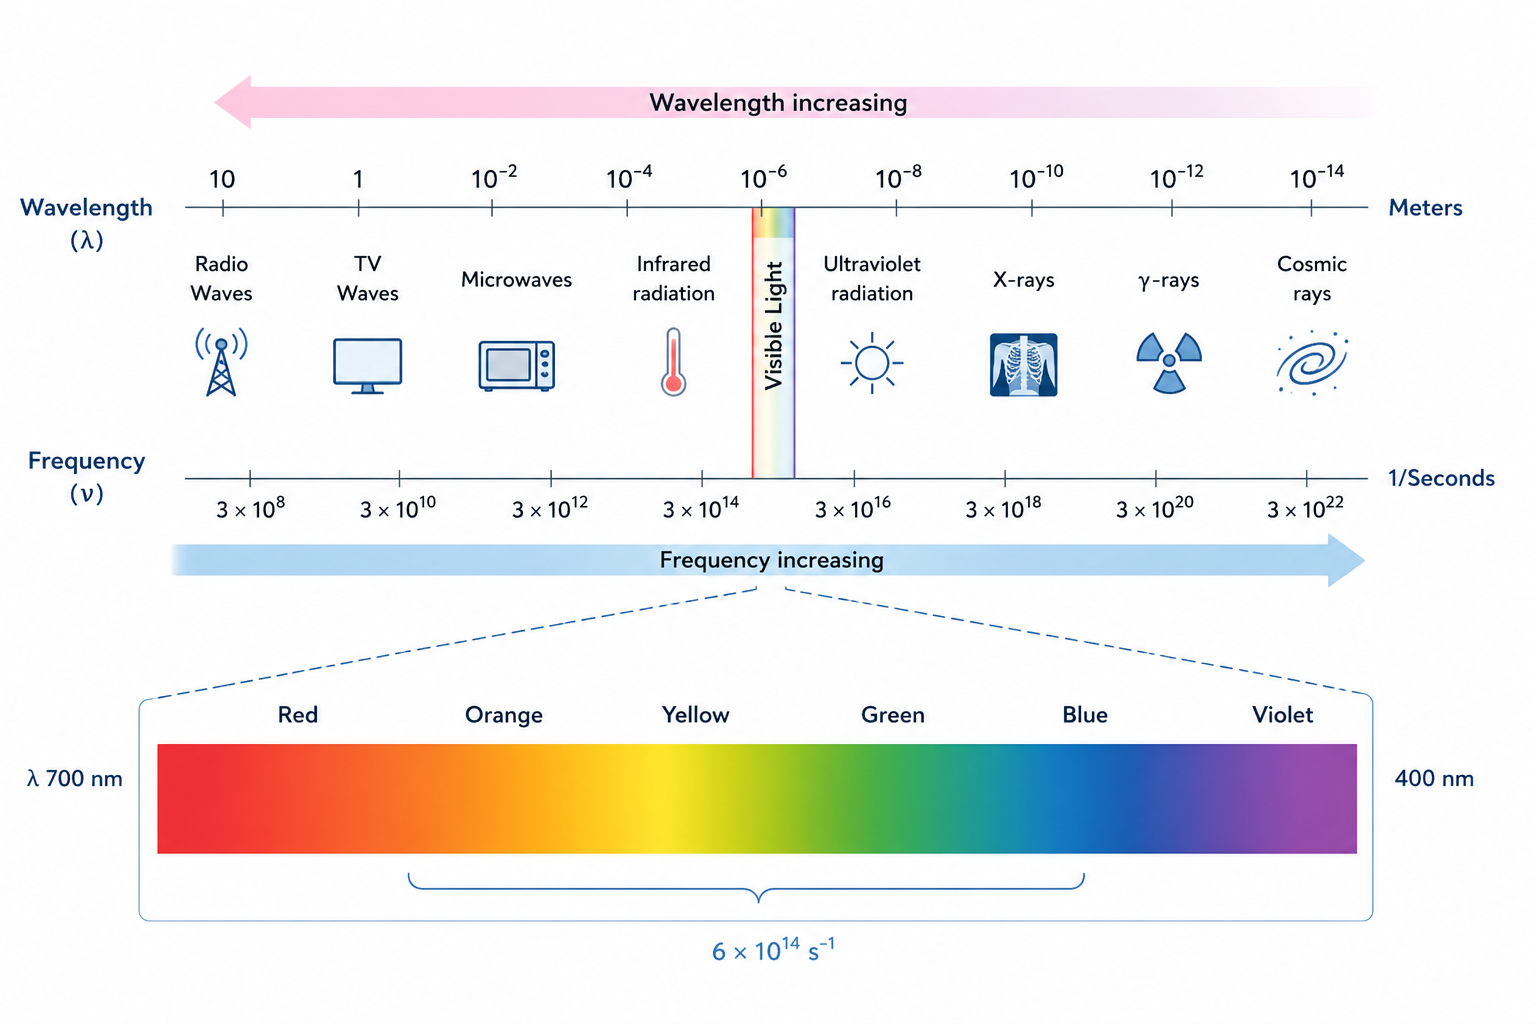
\includegraphics[keepaspectratio]{chapters/../images/image6.electromagneticRanges.png}}
\textbf{גלים אלקטרומגנטיים} הם תופעה גלית שאינה זקוקה לתווך חומרי
להתפשטות --- בניגוד לגלי קול, שזקוקים לאוויר. האור הנראה, קרינת רדיו,
מיקרוגלים, אינפרא-אדום, אולטרה-סגול, רנטגן וקרינת גמא --- כולם אותו
הדבר, הנבדלים זה מזה רק בתדירות ובאורך הגל. קשר בסיסי מאחד את כולם:

\[\lambda \nu = c\]

כאשר \(\lambda\) הוא \textbf{אורך הגל} (wavelength), \(\nu\) היא
\textbf{התדירות} (frequency, ביחידות Hz = \(\text{s}^{-1}\)),
ו-\(c \approx 3 \times 10^8\ \text{m/s}\) היא מהירות האור.

\begin{quote}
\textbf{אזהרה לשוניים:} \(\nu\) היא האות היוונית ``ניו'' --- לא האות
הלטינית v. הן נראות כמעט זהות, אבל מציינות דברים שונים לחלוטין. הבלבול
נפוץ ומביא לטעויות.
\end{quote}

\textbf{האור הנראה} תופס טווח צר ביותר: בין כ-400 nm (סגול) ל-700 nm
(אדום). כל שאר הגלים האלקטרומגנטיים --- בלתי נראים לעיננו.

\textbf{כיצד יודעים שאור הוא גל?} הדרך הפשוטה ביותר: \textbf{עקיפה
והתאבכות} (diffraction and interference). כאשר שני גלים נפגשים, הם
יכולים לחזק זה את זה (בנקודות שבהן שניהם בשיא) או לבטל זה את זה (כאשר
שיא פוגש שפל). התוצאה: פסים מתחלפים של אור וחושך. \textbf{כלל אצבע:} כל
פעם שרואים פסים מתחלפים של אור וחושך --- הוכחה שמדובר בתופעה גלית. \#\#
2.2 ספקטרומי פליטה ובליעה --- החידה הראשונה

\subsection{ספקטרום רציף מול ספקטרום
קווים}\label{ux5e1ux5e4ux5e7ux5d8ux5e8ux5d5ux5dd-ux5e8ux5e6ux5d9ux5e3-ux5deux5d5ux5dc-ux5e1ux5e4ux5e7ux5d8ux5e8ux5d5ux5dd-ux5e7ux5d5ux5d5ux5d9ux5dd}

כאשר אור לבן עובר דרך מנסרה, הוא מתפרק לקשת רציפה של כל הצבעים ---
\textbf{ספקטרום רציף} (continuous spectrum). זה הגיוני: מקור אור לבן
פולט כל אורכי הגל.

אבל כאשר מחממים גז של יסוד טהור (נניח מימן או נתרן) עד שהוא זוהר,
ומעבירים את אורו דרך מנסרה --- מקבלים תוצאה שונה לגמרי: לא קשת רציפה,
אלא \textbf{קווים בודדים} על רקע חשוך. רק אורכי גל ספציפיים מאוד. זהו
\textbf{ספקטרום פליטה} (emission spectrum).

בצד השני: אם שולחים אור לבן \textbf{דרך} גז יסוד טהור, חלק מאורכי הגל
נבלע. התוצאה היא \textbf{ספקטרום בליעה} (absorption spectrum) --- קשת
רציפה עם קווים כהים חסרים בה.
\pandocbounded{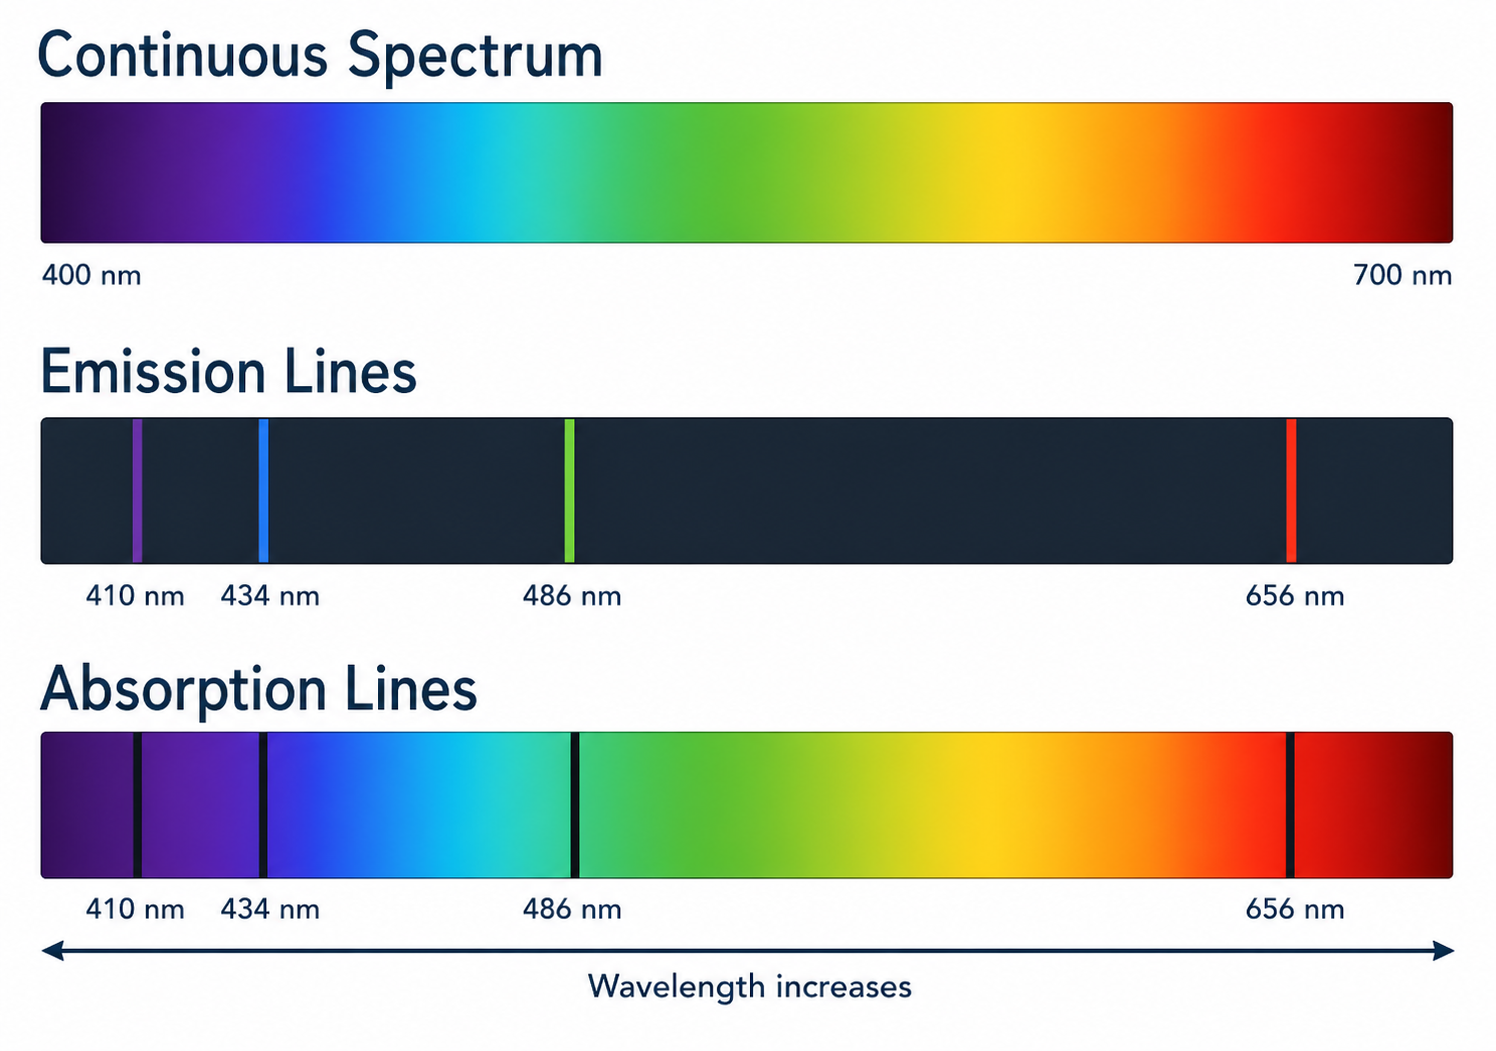
\includegraphics[keepaspectratio]{chapters/../images/image7.EmissionAbsorptionSpectra.png}}
\textbf{תכונה מרכזית:} הקווים הכהים בספקטרום הבליעה נמצאים \textbf{בדיוק
באותם מקומות} כמו הקווים הבהירים בספקטרום הפליטה של אותו יסוד. מה שנבלע
--- נפלט. אותן תדירויות בדיוק.

\subsection{המשמעות}\label{ux5d4ux5deux5e9ux5deux5e2ux5d5ux5ea}

העובדה שאטומים פולטים ובולעים רק תדירויות ספציפיות מלמדת דבר חשוב:
\textbf{בתוך האטום קיים משהו המסוגל לבלוע ולפלוט אנרגיה, וערכי האנרגיה
הללו אינם רציפים --- הם קבועים ומוגדרים לכל יסוד.}

כמו טביעת אצבע: לכל יסוד יש ספקטרום ייחודי משלו. כך ניתן לזהות יסודות
מרחוק --- מהאור של כוכבים, מאש, מפריקה חשמלית. כלי הניתוח הזה נקרא
\textbf{ספקטרוסקופיה}, והוא עדיין אחד הכלים העיקריים בכימיה
ובאסטרונומיה.
\pandocbounded{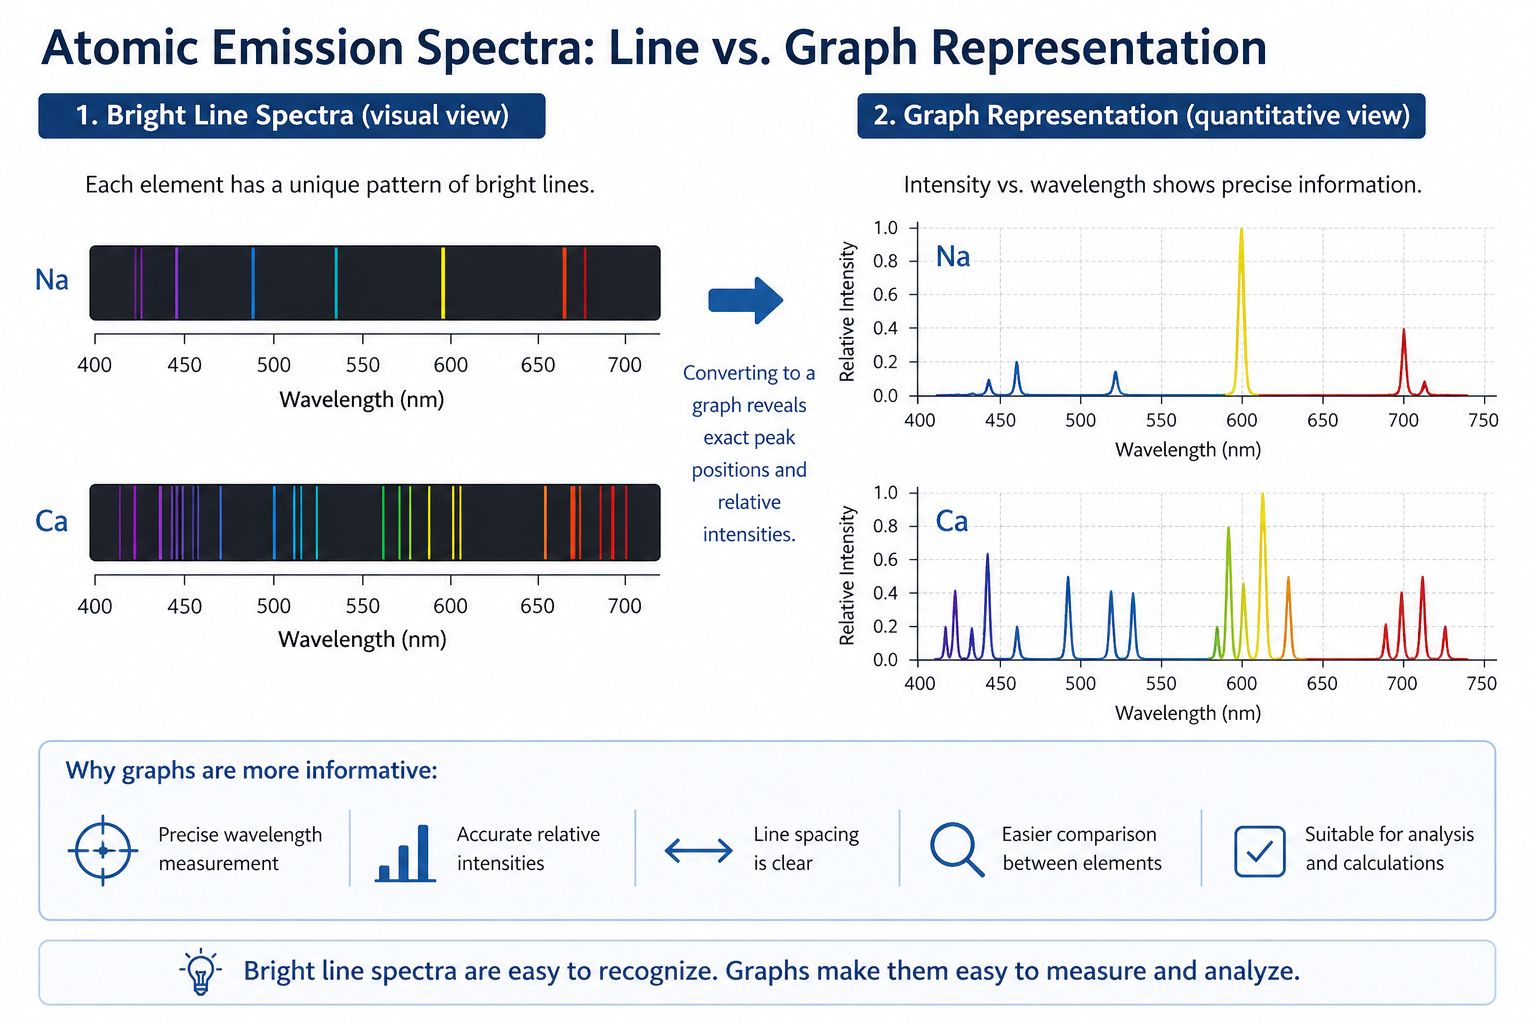
\includegraphics[keepaspectratio]{chapters/../images/image8.FingerprintSpectra.png}}
\#\# 2.3 ספקטרום המימן ונוסחת רידברג

הספקטרום הפשוט ביותר הוא של \textbf{מימן} --- אטום חד-אלקטרוני. ב-1888
הצליח רידברג (Rydberg) לתאר את כל הקווים הספקטרליים של מימן בנוסחה אחת:

\[\frac{1}{\lambda} = R_H \left(\frac{1}{n_1^2} - \frac{1}{n_2^2}\right)\]

כאשר \(R_H = 1.097 \times 10^7\ \text{m}^{-1}\) הוא \textbf{קבוע
רידברג}, ו-\(n_1\), \(n_2\) הם מספרים שלמים חיוביים כלשהם עם
\(n_2 > n_1\).
\pandocbounded{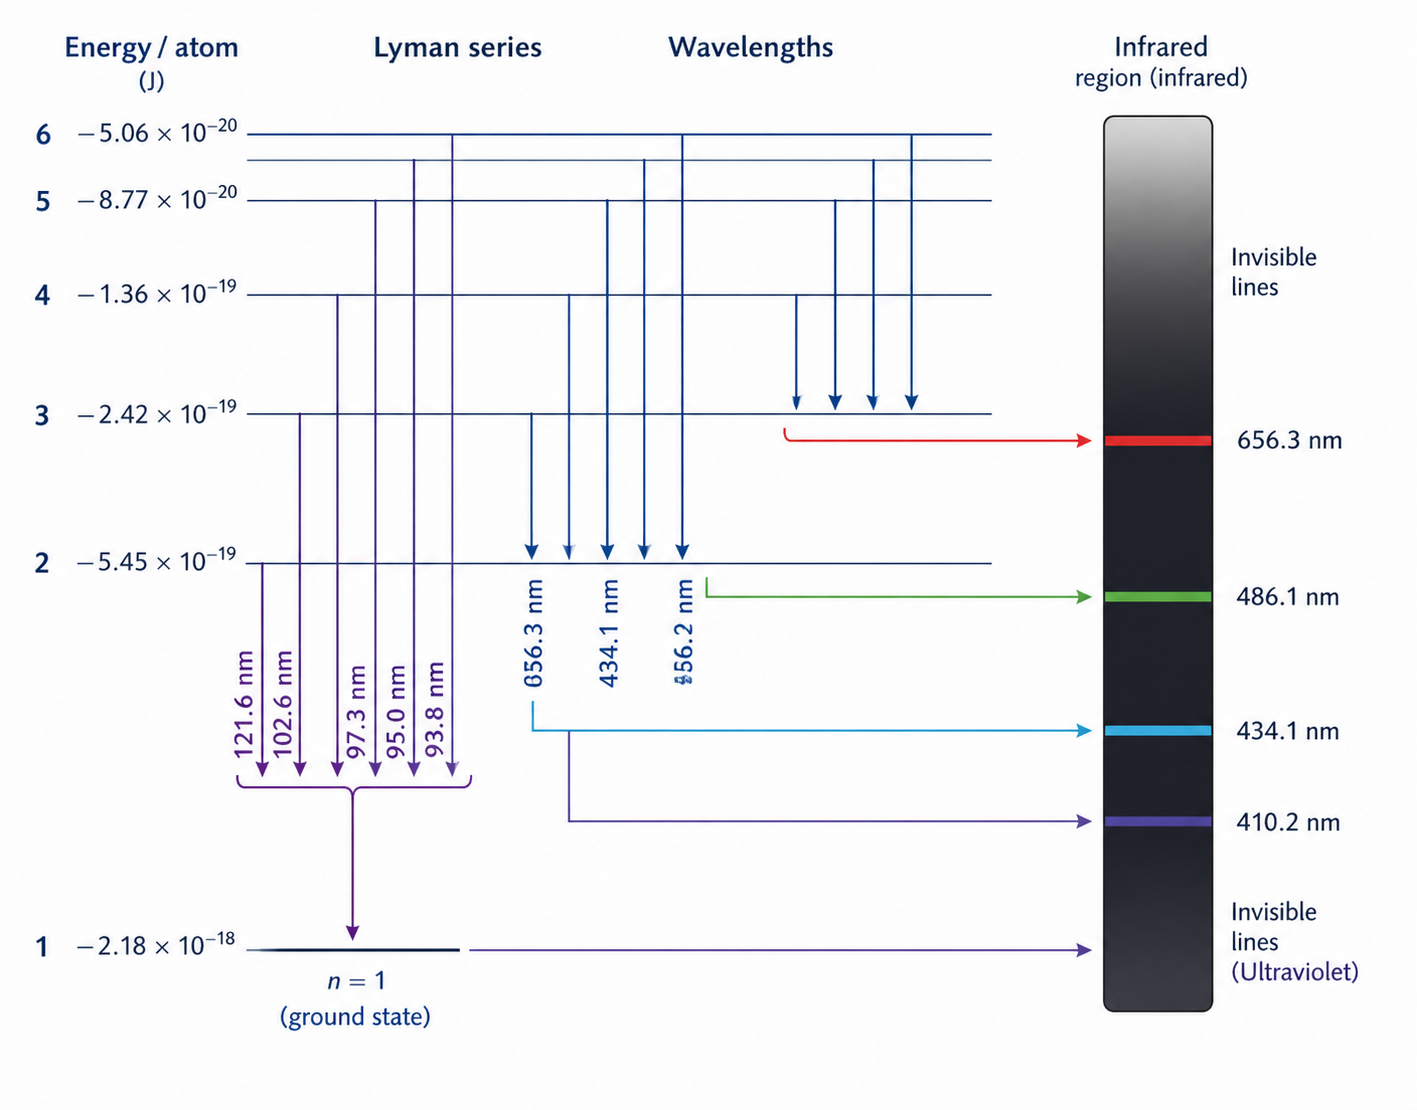
\includegraphics[keepaspectratio]{chapters/../images/image9.Rydberg.png}}
שימו לב: הנוסחה נמצאה \textbf{אמפירית} --- רידברג גילה שהיא עובדת, אבל
לא ידע \emph{למה}. לא הייתה תיאוריה שהסבירה מדוע דווקא מספרים שלמים
מופיעים כאן. זהו אחד הדברים שהמכניקה הקוונטית תסביר לאחר מכן.

לפי ערך \(n_1\) מסווגות משפחות הקווים:

{\def\LTcaptype{none} % do not increment counter
\begin{longtable}[]{@{}lll@{}}
\toprule\noalign{}
משפחה & \(n_1\) & טווח ספקטרלי \\
\midrule\noalign{}
\endhead
\bottomrule\noalign{}
\endlastfoot
סדרת לימן (Lyman) & 1 & אולטרה-סגול \\
סדרת בלמר (Balmer) & 2 & אור נראה \\
סדרת פאשן (Paschen) & 3 & אינפרא-אדום \\
\end{longtable}
}

סדרת בלמר היא הנראית לעין --- ולכן הייתה הראשונה שהתגלתה (1885).

\begin{quote}
\textbf{לחשיבה:} חשבו את אורך הגל של הקו הראשון בסדרת בלמר (\(n_1=2\),
\(n_2=3\)). באיזה צבע הוא?
\end{quote}

כאשר הספקטרוסקופיה שיפרה את דיוקה, התגלה שכל קו שנראה בודד מתפצל בעצם
לכמה קווים קרובים מאוד זה לזה (\textbf{מבנה עדין}, fine structure).
ועוצמות הקווים שונות --- חלקם חזקים וחלקם חלשים. אף אחד מהדברים הללו לא
ניתן להסביר באמצעות נוסחת רידברג --- והם ידרשו הסבר עמוק יותר. \#\# 2.4
כישלון המודל הקלאסי

\subsection{מה הציע המודל
הקלאסי?}\label{ux5deux5d4-ux5d4ux5e6ux5d9ux5e2-ux5d4ux5deux5d5ux5d3ux5dc-ux5d4ux5e7ux5dcux5d0ux5e1ux5d9}

הדגם הקלאסי של האטום (רת'רפורד, 1911) הוא אינטואיטיבי: גרעין במרכז,
אלקטרונים מקיפים אותו כמו כוכבי לכת סביב שמש. משוואת האיזון בין הכוח
הצנטריפוגלי לכוח האלקטרוסטטי (קולון) נותנת רדיוסי מסלול מוגדרים.
\pandocbounded{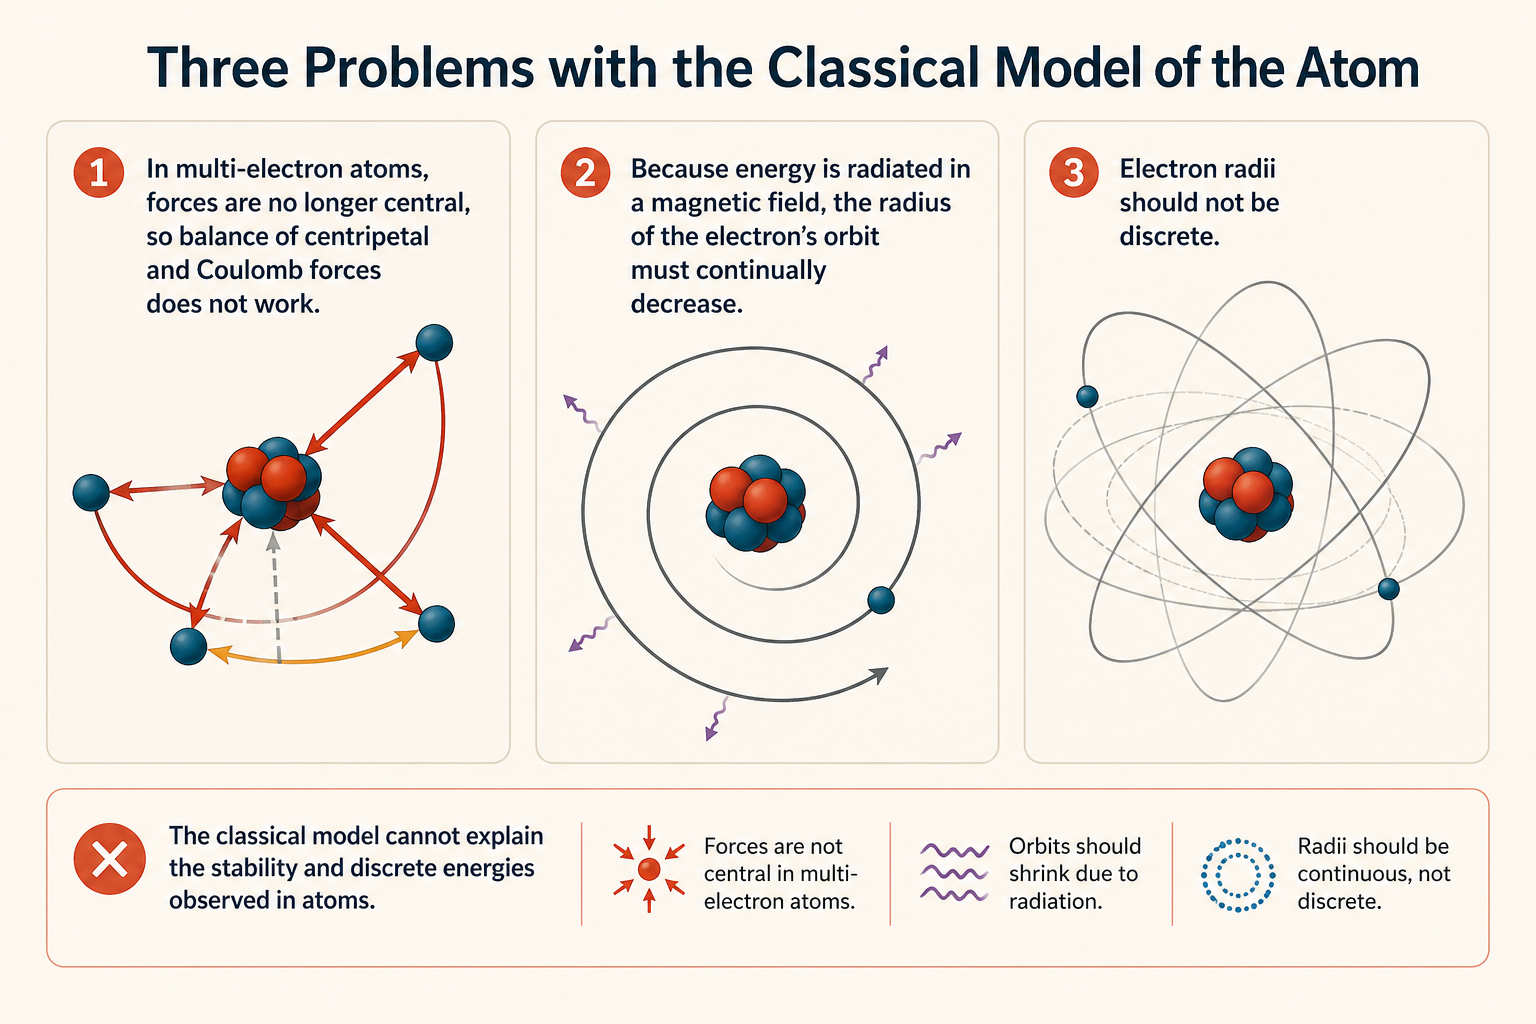
\includegraphics[keepaspectratio]{chapters/../images/image10.ClassicModelFailures.png}}
\#\#\# שלושה כישלונות עקרוניים

\textbf{כישלון ראשון --- קריסת האלקטרון:} תנועה מעגלית היא תנועה
\textbf{מואצת} (כי כיוון המהירות משתנה כל הזמן). לפי המכניקה הקלאסית,
מטען חשמלי מואץ \textbf{חייב} לפלוט קרינה אלקטרומגנטית (\textbf{נוסחת
לארמור}):

\[P = \frac{1}{4\pi\varepsilon_0} \cdot \frac{2e^2 a^2}{3c^3}\]

כאשר \(a\) הוא התאוצה ו-\(P\) הוא הספק הקרינה. אלקטרון שפולט אנרגיה ---
מאבד אנרגיה. אלקטרון שמאבד אנרגיה --- מתקרב לגרעין. חישוב מראה שהאלקטרון
צריך ליפול לגרעין תוך \textbf{\(\sim 10^{-11}\) שנייה}.

אבל אטומים יציבים. אנחנו קיימים. משהו לא עובד.

\textbf{כישלון שני --- ספקטרום רציף:} אם האלקטרון מאבד אנרגיה בהדרגה
ומתקרב לגרעין, רדיוס המסלול משתנה באופן \textbf{רציף}. ולכן גם אורך הגל
של הקרינה הנפלטת צריך להשתנות באופן רציף --- כלומר, הספקטרום צריך להיות
\textbf{רציף}.

אבל אנחנו יודעים שספקטרום המימן מורכב מקווים נפרדים. לא ספקטרום רציף.

\textbf{כישלון שלישי --- אטומים רב-אלקטרוניים:} אפילו אם נתעלם משני
הכישלונות הראשונים, המודל עובד רק לאטום המימן (אלקטרון אחד). ברגע שיש
שני אלקטרונים ומעלה, הם דוחים זה את זה, השדה החשמלי אינו עוד מרכזי ---
והמשוואה מתפרקת. \#\# 2.5 מודל בור --- פתרון חלקי ובעיותיו

\subsection{הפוסטולט של בור
(1913)}\label{ux5d4ux5e4ux5d5ux5e1ux5d8ux5d5ux5dcux5d8-ux5e9ux5dc-ux5d1ux5d5ux5e8-1913}

בור הציע דבר פשוט ואמיץ: \textbf{יש מסלולים יציבים שבהם האלקטרון אינו
פולט קרינה.} הוא לא הסביר \emph{למה} --- פשוט הניח שזה כך.
\pandocbounded{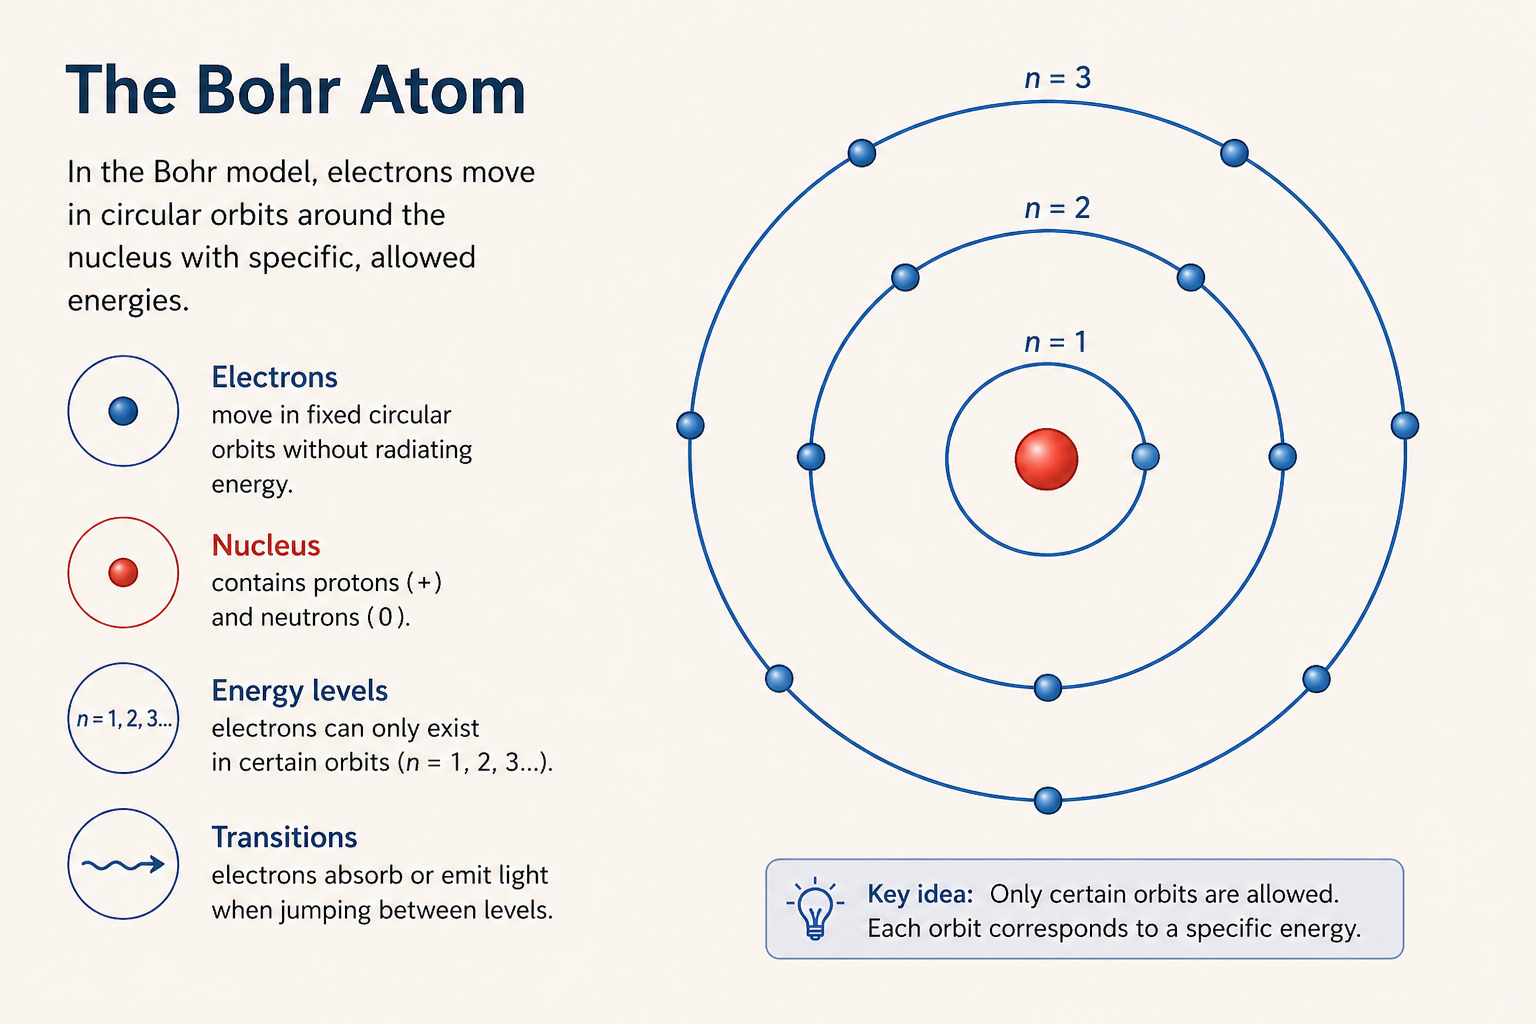
\includegraphics[keepaspectratio]{chapters/../images/image11.BorianAtom.png}}
עם פוסטולט (הנחה ללא הוכחה) זה הצליח לגזור את נוסחת רידברג מתוך תיאוריה,
ולא רק למצוא אותה אמפירית. ערכי \(n\) בנוסחת רידברג התבררו
כ\textbf{מספרים קוונטיים} המגדירים את מסלולי האלקטרון. האנרגיה של מסלול
\(n\):

\[E_n = -\frac{13.6\ \text{eV}}{n^2}\]

כשאלקטרון עובר ממסלול \(n_2\) ל-\(n_1\) (עם \(n_1 < n_2\)), הוא פולט
פוטון עם:

\[\Delta E = E_{n_2} - E_{n_1} = 13.6\ \text{eV} \left(\frac{1}{n_1^2} - \frac{1}{n_2^2}\right)\]

זו בדיוק נוסחת רידברג, עם \(\Delta E = h\nu = hc/\lambda\).

\subsection{מה עדיין לא
עובד?}\label{ux5deux5d4-ux5e2ux5d3ux5d9ux5d9ux5df-ux5dcux5d0-ux5e2ux5d5ux5d1ux5d3}

מודל בור הוא \textbf{``תורת הקוונטים הישנה''} (old quantum theory) ---
הוא עובד למימן, אבל:

\begin{itemize}
\tightlist
\item
  אינו מסביר \emph{מדוע} המסלולים יציבים
\item
  אינו מסביר את המבנה העדין של הקווים
\item
  נכשל לחלוטין לאטומים עם יותר מאלקטרון אחד
\item
  מניח הנחות שרירותיות ללא בסיס תיאורטי
\end{itemize}

תורת הקוונטים הישנה היא אוסף של ``טלאים'' חכמים --- כל אחד מסביר תופעה
מסוימת, אבל יחד הם אינם מהווים תמונה עקבית. פריצת הדרך האמיתית תגיע
ב-1926. \#\# 2.6 האור: גל או חלקיק?

\subsection{עדות לאופי
הגלי}\label{ux5e2ux5d3ux5d5ux5ea-ux5dcux5d0ux5d5ux5e4ux5d9-ux5d4ux5d2ux5dcux5d9}

מאז ניסויי עקיפה של יאנג (Young, 1801) ועד מקסוול (1865), ברור היה שאור
הוא גל --- גל אלקטרומגנטי. עקיפה, התאבכות, קיטוב --- כל אלה הן תכונות
גליות קלאסיות.

\subsection{הפתעה: גוף שחור ואפקט
פוטואלקטרי}\label{ux5d4ux5e4ux5eaux5e2ux5d4-ux5d2ux5d5ux5e3-ux5e9ux5d7ux5d5ux5e8-ux5d5ux5d0ux5e4ux5e7ux5d8-ux5e4ux5d5ux5d8ux5d5ux5d0ux5dcux5e7ux5d8ux5e8ux5d9}

\textbf{גוף שחור} (blackbody) הוא עצם שסופג את כל הקרינה הנופלת עליו.
כשמחממים אותו, הוא פולט קרינה. על פי הפיזיקה הקלאסית, עוצמת הקרינה
הנפלטת צריכה לגדול ללא גבול עם עליית התדירות --- תוצאה אבסורדית שנקראה
\textbf{``קטסטרופת האולטרה-סגול''}.
\pandocbounded{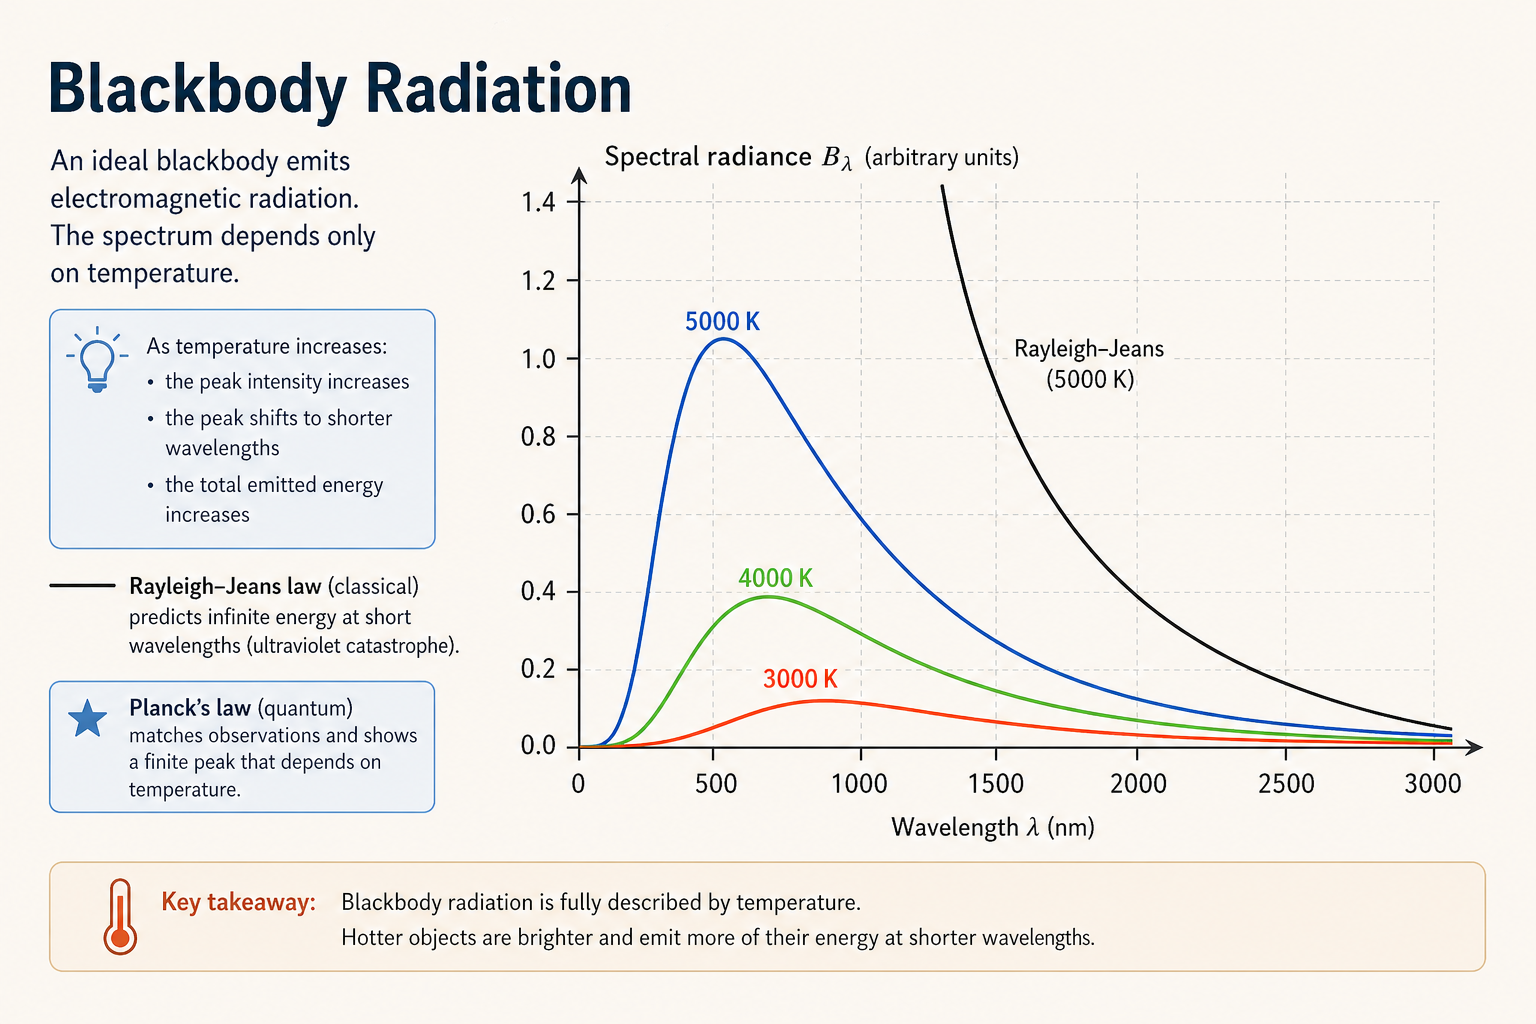
\includegraphics[keepaspectratio]{chapters/../images/image12.BlackBody.png}}
ב-1900 הציע \textbf{פלנק} פתרון מתמטי: אנרגיה אינה יכולה להיפלט בכמויות
רציפות --- רק ב\textbf{חבילות דיסקרטיות}:

\[E = h\nu\]

כאשר \(h = 6.626 \times 10^{-34}\ \text{J·s}\) הוא \textbf{קבוע פלנק}.
פלנק עצמו לא האמין שזה אמיתי --- חשב שזה טריק מתמטי. אבל זה עבד.

ב-1905 הדגים \textbf{איינשטיין} שהרעיון אמיתי: \textbf{האפקט
הפוטואלקטרי} (photoelectric effect) --- כאשר אור פוגע במתכת, הוא מנתק
אלקטרונים. אבל רק אם תדירות האור גבוהה מסף מסוים --- לא משנה כמה עז
האור. זה מוכיח שאנרגיית האור מגיעה ב\textbf{חבילות} (פוטונים), ולא בצורה
רציפה. גל לא היה מתנהג כך.

\textbf{המסקנה:} לאור יש \textbf{דואליות גל-חלקיק} (wave-particle
duality). תכונות מסוימות --- עקיפה, התאבכות --- מוסברות רק אם אור הוא
גל. תכונות אחרות --- אפקט פוטואלקטרי, גוף שחור --- מוסברות רק אם אור הוא
חלקיק. הוא גם וגם, תלוי בשאלה שאנחנו שואלים. \#\# 2.7 האלקטרון: חלקיק או
גל?

\subsection{האלקטרון
כחלקיק}\label{ux5d4ux5d0ux5dcux5e7ux5d8ux5e8ux5d5ux5df-ux5dbux5d7ux5dcux5e7ux5d9ux5e7}

\textbf{ג'וזף ג'יי תומסון} (J.J. Thomson, 1897) גילה שקרני קתודה מורכבות
מחלקיקים קטנים בעלי מטען שלילי --- ה\textbf{אלקטרונים}. מדד את יחס
מטען/מסה שלהם, הוכיח שהם חלקיקים ממשיים. זכה על כך בפרס נובל ב-1906.

\subsection{ההפתעה: האלקטרון גם
גל}\label{ux5d4ux5d4ux5e4ux5eaux5e2ux5d4-ux5d4ux5d0ux5dcux5e7ux5d8ux5e8ux5d5ux5df-ux5d2ux5dd-ux5d2ux5dc}

\textbf{ג'ורג' פגט תומסון} (G.P. Thomson, 1927) --- \textbf{בנו} של
ג'וזף --- שלח אלקטרונים דרך רדיד מתכת דק. התוצאה: \textbf{תבנית עקיפה}
--- בדיוק כמו שמקבלים עם אור. אלקטרונים, שכל העולם ידע שהם חלקיקים, הראו
התנהגות גלית.

גם לאלקטרונים, כמו לאור, יש \textbf{דואליות גל-חלקיק}.
\pandocbounded{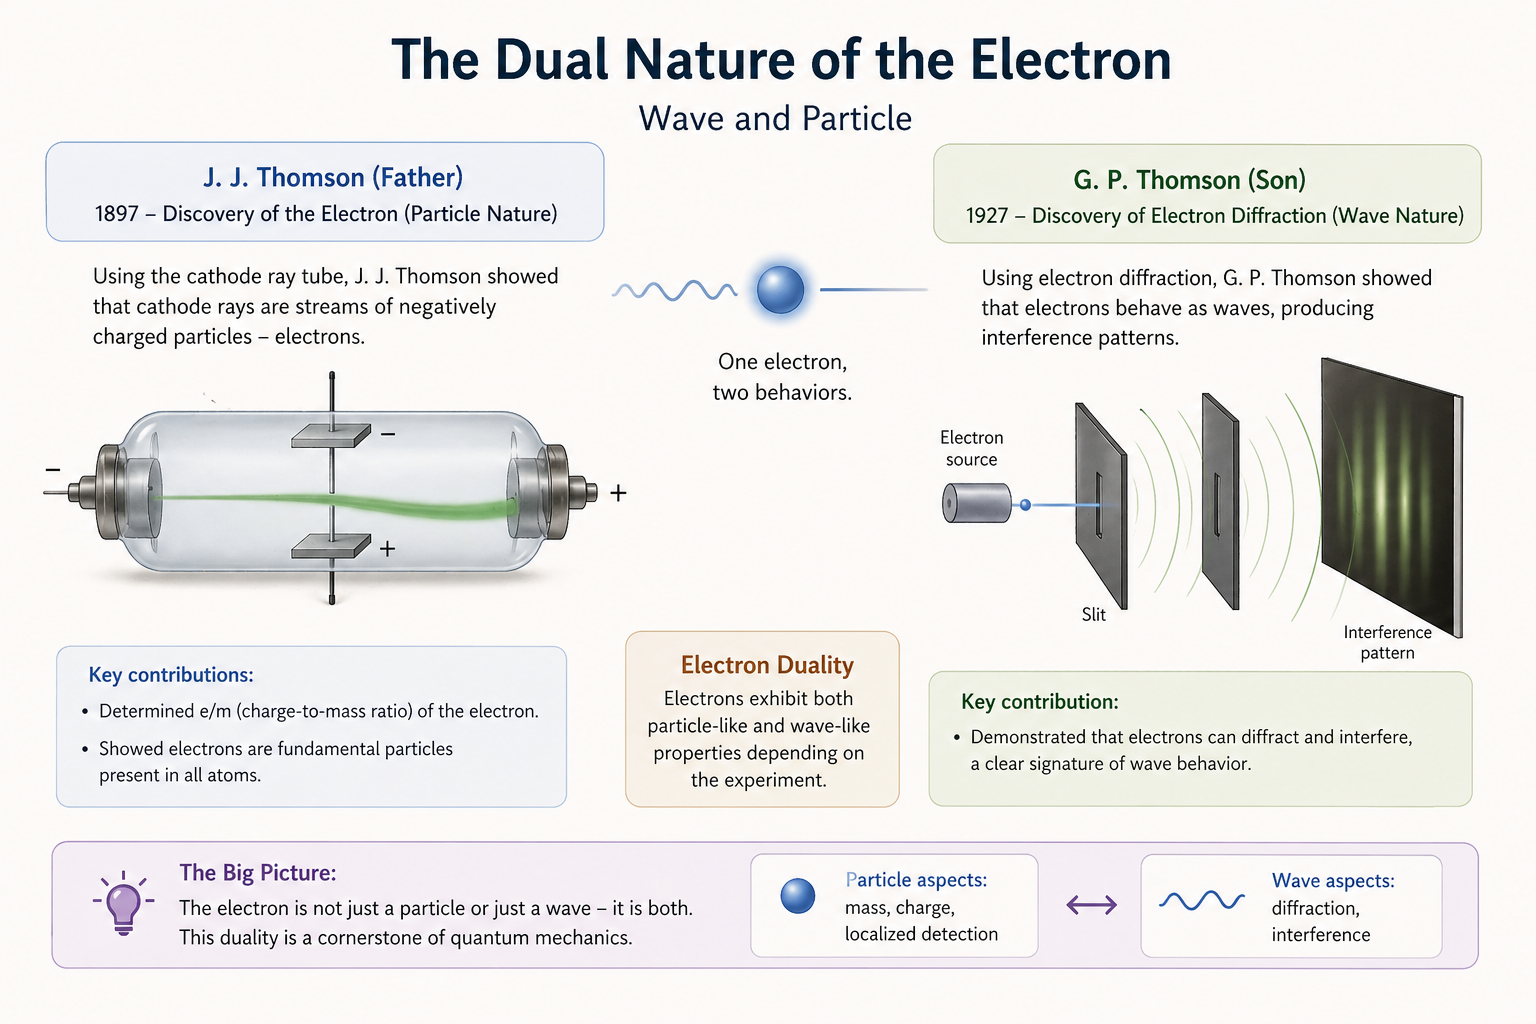
\includegraphics[keepaspectratio]{chapters/../images/image13.ElectronDualism.png}}
\textgreater{} כשם שאביו זכה בפרס נובל על כך שאלקטרון הוא
\textbf{חלקיק}, זכה הבן בפרס נובל (1937) על כך שאלקטרון הוא \textbf{גל}.
שניהם צדקו. \#\# 2.8 ניסוי שטרן-גרלך --- המדידה משנה את הנמדד

\subsection{הניסוי}\label{ux5d4ux5e0ux5d9ux5e1ux5d5ux5d9}

ב-1922 ביצעו שטרן (Stern) וגרלך (Gerlach) ניסוי פשוט לכאורה: שלחו קרן של
אטומי כסף (Ag) דרך שדה מגנטי לא-אחיד. לאטומי כסף יש \textbf{מומנט מגנטי}
(magnetic moment) --- הם מגיבים לשדה מגנטי כמו מגנטים זעירים.

\textbf{תחזית קלאסית:} המגנטים הזעירים מכוונים לכיוונים שרירותיים שונים
→ השדה יסיט כל אטום בכמות שונה → הקרן תתרחב ל\textbf{פס רציף}.

\textbf{תוצאה בפועל:} הקרן התפצלה בדיוק \textbf{לשני כתמים} --- אחד
למעלה ואחד למטה. לא פס רציף, לא שלושה כתמים --- שניים בדיוק, עם עוצמה
שווה.

\subsection{המשמעות הראשונה:
דיסקרטיות}\label{ux5d4ux5deux5e9ux5deux5e2ux5d5ux5ea-ux5d4ux5e8ux5d0ux5e9ux5d5ux5e0ux5d4-ux5d3ux5d9ux5e1ux5e7ux5e8ux5d8ux5d9ux5d5ux5ea}

המומנט המגנטי אינו יכול לקבל ערכים רציפים --- רק \textbf{שניים} (מצב
``מעלה'' ומצב ``מטה''). זוהי \textbf{קוונטיזציה} (quantization): התכונה
הפיזיקלית מקבלת רק ערכים בדידים, לא ערך כלשהו.

המילה ``דיסקרטי'' (discrete) בעברית מדעית פירושה \textbf{קצוב, מופרד,
מובדל} --- לא ``סודי'' כפי שלפעמים טועים לחשוב.
\pandocbounded{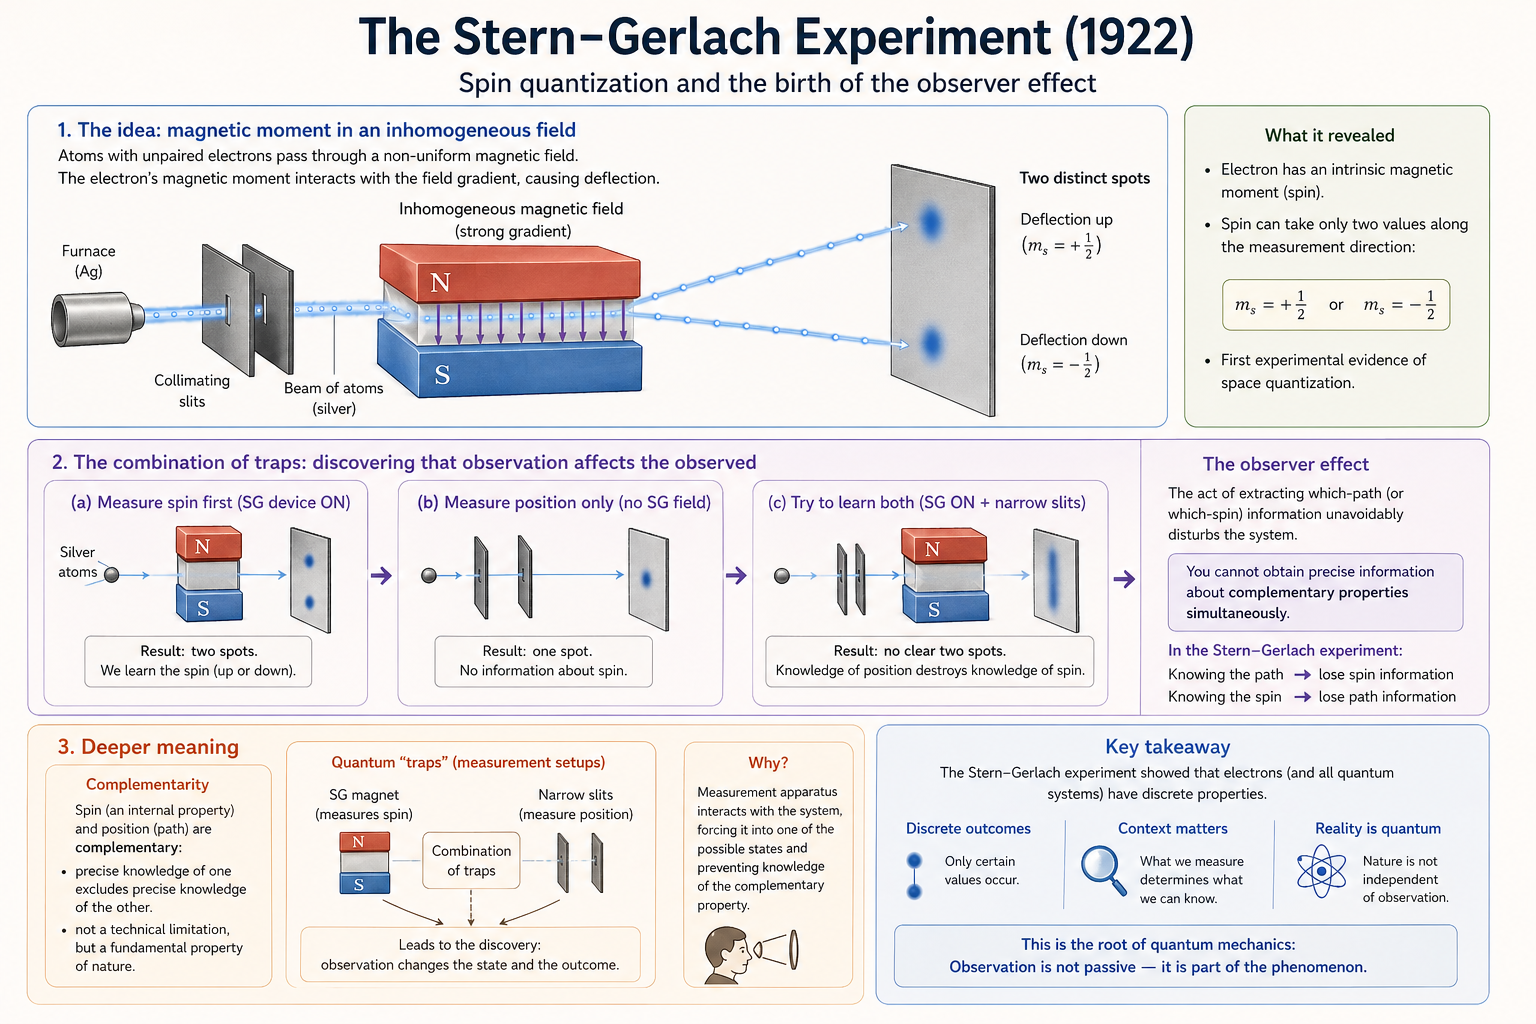
\includegraphics[keepaspectratio]{chapters/../images/image14.SternGerlach.png}}
\#\#\# המשמעות השנייה: המדידה משנה את הנמדד

שטרן וגרלך ביצעו ניסוי המשך: לקחו את האטומים שנסטו למעלה (``מצב מעלה''),
והעבירו אותם דרך מכשיר שני, \textbf{מסובב ב-90°}.

תחזית אינטואיטיבית: כיוון שסיננו את מצב ``מעלה'', כולם אמורים להישאר
``מעלה'' גם במכשיר השני.

\textbf{תוצאה בפועל:} שוב שני כתמים שווים --- 50\% ``מעלה'', 50\%
``מטה''. כאילו האטומים ``שכחו'' שסוננו.

ההסבר: \textbf{כשמדדנו עם המכשיר הראשון, שינינו את מצב האטומים.} המדידה
בכיוון אחד מחקה את המידע על הכיוון הניצב. אין דרך ``להציץ'' על מצב האטום
מבלי להשפיע עליו.

זוהי אחת ההשלכות העמוקות ביותר של מכניקת הקוונטים: \textbf{אין מציאות
קוונטית עצמאית שאנחנו רק ``מגלים''. המדידה היא חלק מהתהליך.} \#\# 2.9
גלי דה-ברויי --- האחדה מתמטית

\subsection{הרעיון}\label{ux5d4ux5e8ux5e2ux5d9ux5d5ux5df}

\pandocbounded{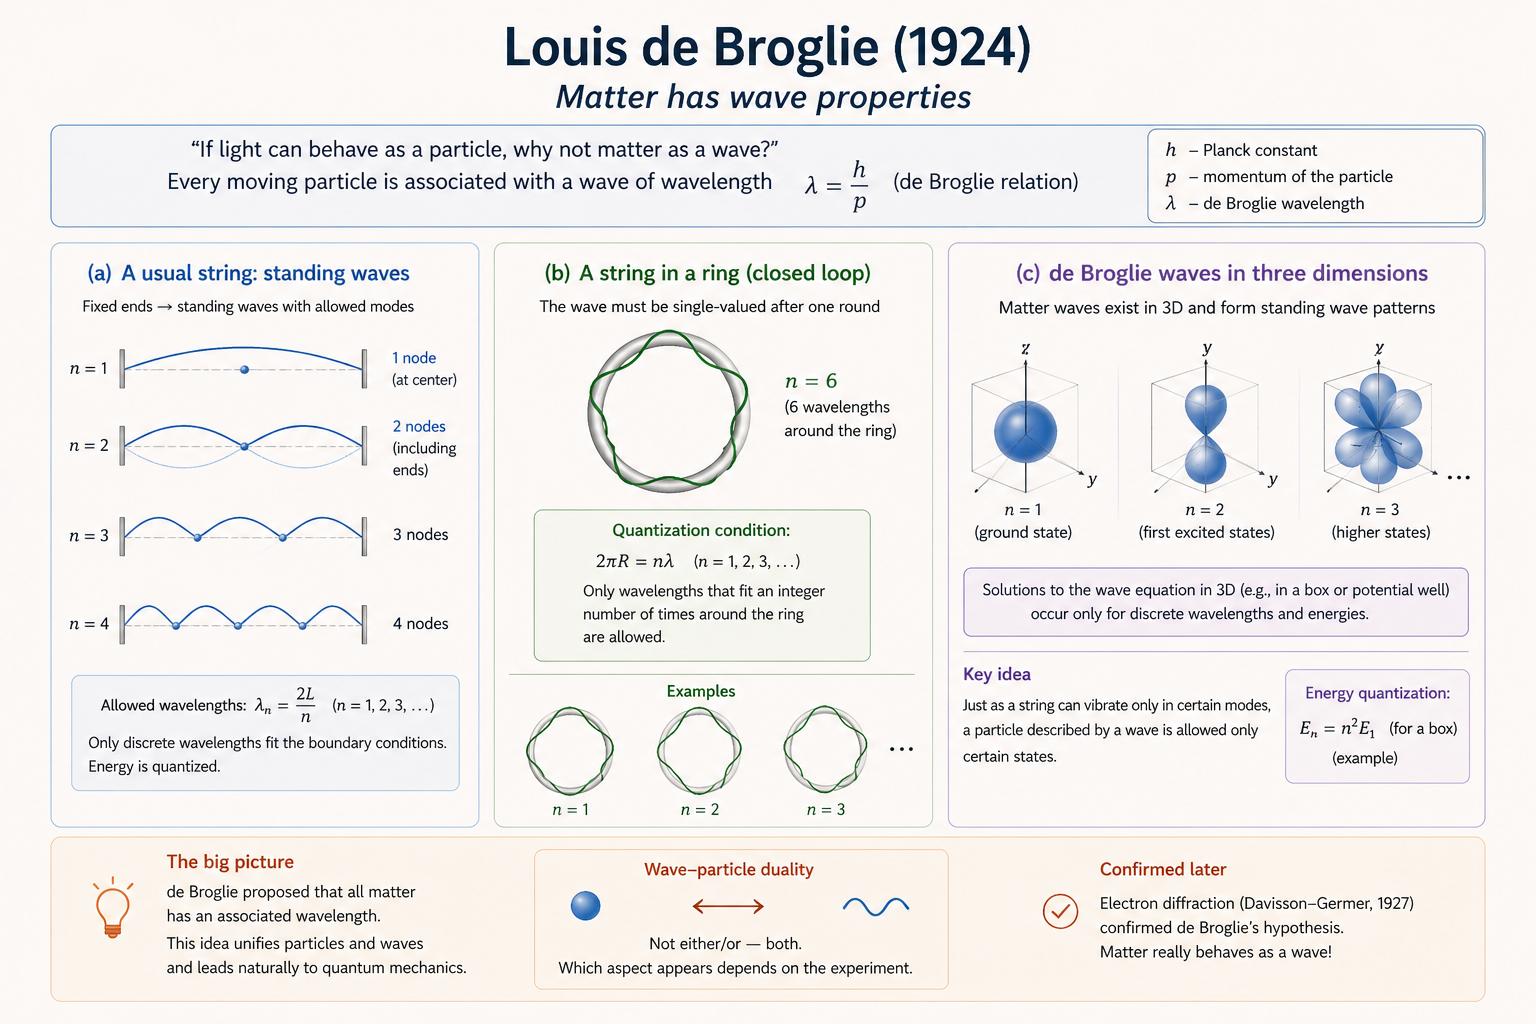
\includegraphics[keepaspectratio]{chapters/../images/image15.DeBroglie.png}}
ב-1924 --- שלוש שנים לפני שתומסון הבן הדגים זאת ניסויית --- הציע לואי
דה-ברויי (de Broglie) בעבודת הדוקטורט שלו שהדואליות אינה ייחודית לאור:
\textbf{לכל חלקיק יש אורך גל}.

הטיעון המתמטי פשוט. מצד אחד, לפוטון (חלקיק אור) יש אנרגיה לפי פלנק:
\[E = h\nu\]

מצד שני, לפי יחסיות איינשטיין, לחלקיק בעל מסה יש אנרגיה: \[E = mc^2\]

השוואה: \(mc^2 = h\nu = hc/\lambda\), ולכן:
\[\lambda = \frac{h}{mc} = \frac{h}{p}\]

כאשר \(p = mc\) הוא המומנטום. כלומר: \textbf{לכל חלקיק עם מומנטום \(p\)
יש אורך גל \(\lambda = h/p\).}

\subsection{מה זה אומר לגבי
האלקטרון?}\label{ux5deux5d4-ux5d6ux5d4-ux5d0ux5d5ux5deux5e8-ux5dcux5d2ux5d1ux5d9-ux5d4ux5d0ux5dcux5e7ux5d8ux5e8ux5d5ux5df}

אם האלקטרון הוא גל, ואם הוא נע במסלול מעגלי סביב הגרעין, אז כדי שהגל
``יסגור'' את עצמו בצורה קוהרנטית --- כלומר, שהגל בנקודת ההתחלה יתאים לגל
בנקודת הסיום --- מספר הגלים במסלול חייב להיות \textbf{שלם}:

\[2\pi r = n\lambda = n\frac{h}{p}\]

זוהי בדיוק תנאי הכימות של בור! הרדיוסים היציבים שבור הניח כפוסטולט ---
יוצאים עכשיו מתוך דרישה פיזיקלית: \textbf{גל עומד על מסלול סגור.}

\begin{quote}
\emph{``התיאוריה שלך מטורפת, אבל לא מטורפת מספיק כדי להיות נכונה.''} ---
ניילס בור, כשרעיון דה-ברויי הוצג בפניו לראשונה
\end{quote}

הפעם בור טעה. כעבור שלוש שנים הדגים תומסון הבן שאלקטרונים מייצרים תבניות
עקיפה --- בדיוק כמו גלים. \#\# סיכום --- מה שאספנו

עד לנקודה זו ידוע לנו:

ניסויים מצביעים על שלושה עקרונות שהפיזיקה הקלאסית לא יכולה להכיל:

\textbf{1. קוונטיזציה:} תכונות פיזיקליות (אנרגיה, מומנט מגנטי) מקבלות רק
ערכים בדידים --- לא ערך כלשהו.

\textbf{2. דואליות גל-חלקיק:} גם אור וגם אלקטרונים מתנהגים לפעמים כגלים
ולפעמים כחלקיקים, תלוי בניסוי שמבצעים.

\textbf{3. השפעת המדידה:} מדידה של תכונה קוונטית אחת משנה את מצב המערכת
ומשמידה מידע על תכונות אחרות.

שלושה עקרונות אלו אינם ``תופעות מוזרות'' --- הם בסיס של תורה שלמה ועקבית
שנבנתה בשנים 1926--1930. הפרק הבא יציג אותה.

\bookmarksetup{startatroot}

\chapter{פרק 3 --- מכניקת הקוונטים: השפה החדשה של
הפיזיקה}\label{ux5e4ux5e8ux5e7-3-ux5deux5dbux5e0ux5d9ux5e7ux5ea-ux5d4ux5e7ux5d5ux5d5ux5e0ux5d8ux5d9ux5dd-ux5d4ux5e9ux5e4ux5d4-ux5d4ux5d7ux5d3ux5e9ux5d4-ux5e9ux5dc-ux5d4ux5e4ux5d9ux5d6ux5d9ux5e7ux5d4}

\section{מבוא: מ''טלאים'' לתיאוריה
שלמה}\label{ux5deux5d1ux5d5ux5d0-ux5deux5d8ux5dcux5d0ux5d9ux5dd-ux5dcux5eaux5d9ux5d0ux5d5ux5e8ux5d9ux5d4-ux5e9ux5dcux5deux5d4}

בפרק הקודם ראינו שהפיזיקה הקלאסית נכשלת מול העולם האטומי, ושניסיונות
התיקון --- מודל בור, גלי דה-ברויי --- עובדים חלקית אך אינם מהווים
תיאוריה עקבית. כל פתרון יצר בעיה חדשה; כל הסבר דרש הנחה שרירותית.

בין 1926 ל-1930 השתנה הכל. \textbf{שרדינגר} (Schrödinger),
\textbf{היזנברג} (Heisenberg), \textbf{דיראק} (Dirac) ואחרים גיבשו
תיאוריה חדשה ושלמה --- \textbf{מכניקת הקוונטים} (quantum mechanics). היא
אינה ``תיקון'' לפיזיקה הקלאסית, אלא השקפת עולם שונה לחלוטין.

כמה מתמטיקה נדרשת להבין אותה לחלוטין? למשל במכון הטכנולוגי של מסצ'וסטס
(MIT): חדו''א, פיזיקה 2 ו-3, ואז שלושה קורסים של פיזיקה קוונטית בשנים
ב'--ג'. \textbf{בקורס הנוכחי} לא מתיימרים להגיע לשם. המטרה היא הבנה
מושגית ויכולת לעבוד עם הכלים המרכזיים. \#\# 3.1 שבעת הפוסטולטים

מכניקת הקוונטים מבוססת על מספר עקרונות יסוד --- \textbf{פוסטולטים} ---
שאינם נגזרים מכלום שקדם להם. הם פשוט הנחות שהתבררו נכונות. מתמטית, כל
הפוסטולטים עקביים; פיזיקלית, חלקם מאתגרים את האינטואיציה.

\subsection{פוסטולט 1 --- דואליות
גל-חלקיק}\label{ux5e4ux5d5ux5e1ux5d8ux5d5ux5dcux5d8-1-ux5d3ux5d5ux5d0ux5dcux5d9ux5d5ux5ea-ux5d2ux5dc-ux5d7ux5dcux5e7ux5d9ux5e7}

כל חלקיק הוא גל, וכל גל הוא חלקיק. כל אובייקט קוונטי מתואר על ידי
\textbf{פונקציית גל} (wave function):

\[\psi(x_1, \ldots, x_N, t)\]

המוגדרת על \(N\) קואורדינטות ועל הזמן \(t\). חלופית, ניתן לתאר אותו
כ\textbf{וקטור מצב}:

\[|\psi\rangle \equiv \begin{pmatrix} a_1 \ a_2 \ a_3 \ \vdots \end{pmatrix}\]

כאשר \(a_i\) הם ערכי תכונות. שתי הגישות --- פונקציית גל ווקטור ---
שקולות מתמטית ומשמשות לסירוגין.

\subsection{פוסטולט 2 ---
דיסקרטיות}\label{ux5e4ux5d5ux5e1ux5d8ux5d5ux5dcux5d8-2-ux5d3ux5d9ux5e1ux5e7ux5e8ux5d8ux5d9ux5d5ux5ea}

המצבים הקוונטיים הם \textbf{דיסקרטיים} (discrete) --- קצובים, מופרדים,
מובדלים. לא כל ערך אפשרי, אלא רק ערכים מוגדרים.

הערה לשונית: ``דיסקרטי'' במדע פירושו \emph{מובחן ומופרד} --- לא ``סודי''
כפי שלפעמים טועים לחשוב בעברית יומיומית. אנגלית: \emph{discrete} (לא
\emph{discreet}).

\subsection{פוסטולט 3 ---
סופרפוזיציה}\label{ux5e4ux5d5ux5e1ux5d8ux5d5ux5dcux5d8-3-ux5e1ux5d5ux5e4ux5e8ux5e4ux5d5ux5d6ux5d9ux5e6ux5d9ux5d4}

חלקיק קוונטי מהווה \textbf{סופרפוזיציה} (superposition) --- ``סכום'' ---
של \textbf{כל} המצבים הקוונטיים האפשריים, בו-זמנית. הוא אינו ``במצב אחד
שאנחנו לא יודעים איזה'' --- הוא ממש בכולם. מבחינת שתי התצוגות של אובייקט
קוונטי (פונקציית גל ווקטור מצב), ניתן לומר שסופרפוזיציה היא התאבכות של
כל הגלים האפשריים או אחרת שהיא סכום ווקטורי של וקטורי מצב במרחב מופשט.

\textbf{אנלוגיה:} מסך RGB בנוי משלוש שכבות צבע --- אדום, ירוק וכחול. כל
פיקסל הוא ``סופרפוזיציה'' של שלושת הצבעים בו-זמנית; מה שרואים הוא התוצאה
המשולבת. מתמטית, הסופרפוזיציה היא סכום (או אינטגרל) של כל המצבים
האפשריים, כל אחד עם מקדם.

\subsection{פוסטולט 4 --- הסתברות
בלבד}\label{ux5e4ux5d5ux5e1ux5d8ux5d5ux5dcux5d8-4-ux5d4ux5e1ux5eaux5d1ux5e8ux5d5ux5ea-ux5d1ux5dcux5d1ux5d3}

לא ניתן לקבוע \emph{ערך} של תכונה קוונטית --- רק את \textbf{ההסתברות}
לקבל כל ערך אפשרי. בעולם הקלאסי, לכל חלקיק יש מיקום ומהירות מוגדרים ---
גם אם אנחנו לא יודעים אותם. בעולם הקוונטי, אין ערך מוגדר \emph{לפני
המדידה}. זה לא חוסר ידע --- זה מצב פיזיקלי אמיתי.

\subsection{פוסטולט 5 --- חשבון כל
ההסתברויות}\label{ux5e4ux5d5ux5e1ux5d8ux5d5ux5dcux5d8-5-ux5d7ux5e9ux5d1ux5d5ux5df-ux5dbux5dc-ux5d4ux5d4ux5e1ux5eaux5d1ux5e8ux5d5ux5d9ux5d5ux5ea}

יש להתחשב \textbf{בכל} ההסתברויות --- אסור להתעלם מאף אחת. בפיזיקה
קלאסית מותר להתעלם מאפשרויות בעלות הסתברות זניחה. בפיזיקה קוונטית ---
לא. גם מסלול שנראה ``בלתי אפשרי'' תורם לתוצאה הסופית.

זה הבסיס לתופעת \textbf{מנהור קוונטי} (quantum tunneling): חלקיק יכול
לעבור דרך מחסום אנרגטי שבפיזיקה קלאסית היה בלתי עביר. הסיבה: יש הסתברות
שאינה אפסית שהוא ``יהיה'' בצד השני --- ואסור להתעלם ממנה.

\subsection{פוסטולט 6 --- המדידה משנה את
הנמדד}\label{ux5e4ux5d5ux5e1ux5d8ux5d5ux5dcux5d8-6-ux5d4ux5deux5d3ux5d9ux5d3ux5d4-ux5deux5e9ux5e0ux5d4-ux5d0ux5ea-ux5d4ux5e0ux5deux5d3ux5d3}

כאשר מודדים תכונה קוונטית, המדידה \textbf{``הורסת''} (collapses) את
הסופרפוזיציה --- מכל המצבים האפשריים, והמערכת ``קופצת'' לאחד מהם. לאחר
המדידה, המערכת כבר אינה במצב הסופרפוזיציה המקורי.

\textbf{אנלוגיה:} כאשר מנסים להציץ לחדר שבו ילדים משתוללים, ברגע שפותחים
את הדלת הם מסדרים את עצמם. לא ניתן לראות ``את האמת הלא מושפעת״ בגלל
ההצצה עצמה.

המשמעות: \textbf{אין מציאות קוונטית עצמאית שאנחנו ``מגלים'' במדידה ---
המדידה היא חלק מהתהליך.} זה שונה לחלוטין מהפיזיקה הקלאסית, שם המדידה רק
חושפת ערך שהיה קיים לפניה.

\subsection{פוסטולט 7 --- שזירה
קוונטית}\label{ux5e4ux5d5ux5e1ux5d8ux5d5ux5dcux5d8-7-ux5e9ux5d6ux5d9ux5e8ux5d4-ux5e7ux5d5ux5d5ux5e0ux5d8ux5d9ux5ea}

שני חלקיקים קוונטיים שיצרו אינטראקציה יכולים להישאר \textbf{שזורים}
(entangled) --- כך שמדידה של האחד משפיעה מיידית על המצב של השני, לא משנה
כמה רחוקים הם זה מזה. אינשטיין כינה זאת ``פעולה מפחידה מרחוק'' (spooky
action at a distance) ולא האמין בה. ניסויים הוכיחו שהיא אמיתית.

שזירה קוונטית היא הבסיס של \textbf{מחשוב קוונטי} --- מחשבים המנצלים את
הסופרפוזיציה והשזירה כדי לבצע חישובים שמחשב קלאסי אינו יכול לבצע
ביעילות. \textgreater{} \textbf{הערה מעשית:} ניתן לחיות ולעבוד היטב מבלי
להבין לעומק את כל הפוסטולטים. אנחנו עושים שימוש יומיומי בפירות של
תיאוריות שאיננו מבינים לגמרי --- בדיוק כמו שרוב האנשים מפעילים תנור
מיקרוגל ללא הבנה של האלקטרודינמיקה שמאחוריו. \#\# 3.2 פירושים של מכניקת
הקוונטים --- שאלות פילוסופיות פתוחות

המתמטיקה של מכניקת הקוונטים עקבית ומדויקת. אבל \emph{מה זה אומר}? כאן
הדעות חלוקות --- ויש כמאה הצעות שונות. להלן המרכזיות:

\textbf{פירוש קופנהגן} (Bohr \& Heisenberg, 1927): השאלה ``איפה היה
החלקיק לפני שמדדתי?'' היא חסרת משמעות. אין מציאות עצמאית מחוץ לתצפית.
\emph{``המציאות נמצאת בתצפית ולא באלקטרון.''} זהו הפירוש הנפוץ ביותר
בקרב פיזיקאים מעשיים.

\textbf{פירוש עולמות מרובים} (Everett, 1957): כל מדידה ``מפצלת'' את
היקום לענפים מקבילים. בענף אחד המדידה נתנה ערך A, בענף אחר --- ערך B.
הסופרפוזיציה ממשית; אנחנו רואים רק ענף אחד. מושאל מאוד מסרטי מדע בדיוני
--- אך גם לוקח אותה ברצינות חלק מהפיזיקאים.

\textbf{היגיון קוונטי} (von Neumann, 1936): ההיגיון הבינארי הקלאסי (``כן
או לא'') אינו תקף בעולם הקוונטי. חוק השלישי הנשלל (\emph{tertium non
datur} --- ``אין שלישי'') אינו עובד. זה הבסיס התיאורטי של מחשוב קוונטי.

\textbf{``Shut up and calculate''} (Mermin): הגישה הפרגמטית הנפוצה ביותר
\emph{בפועל} --- אל תנסה להבין מה זה ``אומר'', פשוט עשה את החישובים ועשה
שימוש בתוצאות.

\pandocbounded{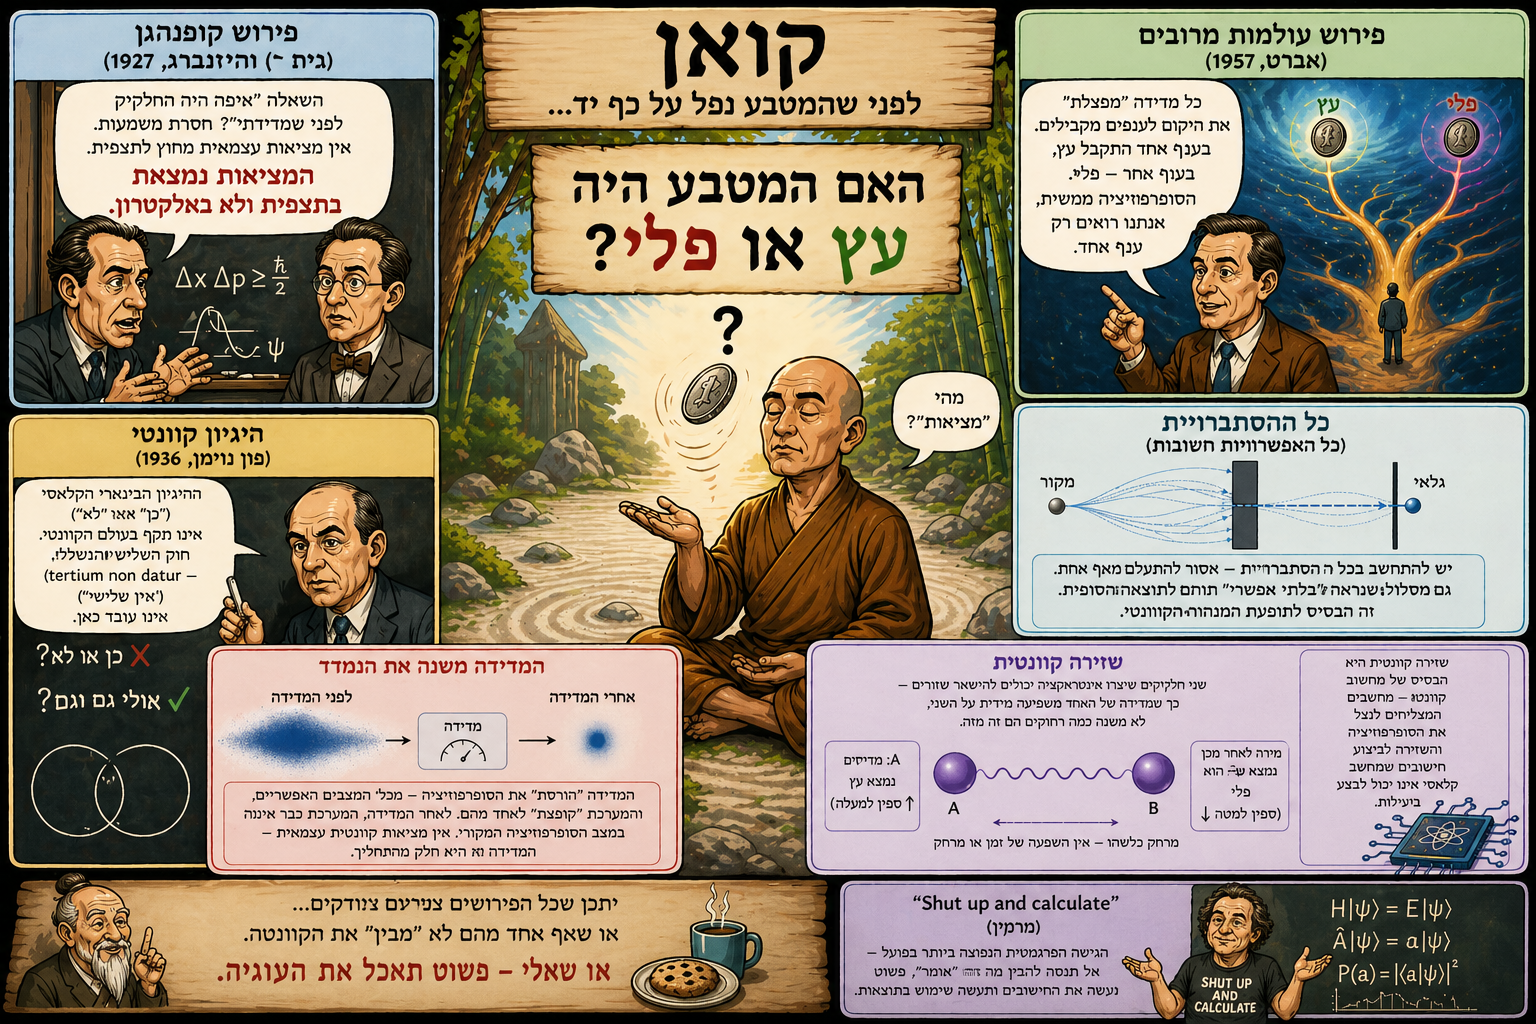
\includegraphics[keepaspectratio]{chapters/../images/image16.Koan.png}}

\begin{quote}
\textbf{לצורכי הקורס:} הפירוש הפילוסופי אינו נושא המבחן. המספרים
הקוונטיים ויישומם --- כן. \#\# 3.3 אופרטורים, פונקציות עצמיות וערכים
עצמיים
\end{quote}

\subsection{מהו
אופרטור?}\label{ux5deux5d4ux5d5-ux5d0ux5d5ux5e4ux5e8ux5d8ux5d5ux5e8}

\textbf{אופרטור} הוא כלל הממיר \emph{פונקציה} אחת לפונקציה אחרת ---
בניגוד לפונקציה רגילה שממירה \emph{מספר} למספר.

דוגמאות לאופרטורים מוכרים: \(\frac{d}{dx}\) (נגזרת), \(\int dx\)
(אינטגרל), \(\sqrt{\phantom{x}}\) (שורש), כפל בקבוע ועוד. כולם פועלים על
פונקציות ומחזירים פונקציות.

\[\hat{A}f(x) = g(x)\]

למשל: \(\frac{d}{dx}[\sin x] = \cos x\) --- האופרטור ``נגזרת'' פועל על
\(\sin x\) ומחזיר \(\cos x\).

\subsection{פונקציות עצמיות וערכים
עצמיים}\label{ux5e4ux5d5ux5e0ux5e7ux5e6ux5d9ux5d5ux5ea-ux5e2ux5e6ux5deux5d9ux5d5ux5ea-ux5d5ux5e2ux5e8ux5dbux5d9ux5dd-ux5e2ux5e6ux5deux5d9ux5d9ux5dd}

\textbf{אופרטור לינארי} מיוחד: כאשר האופרטור פועל על פונקציה מסוימת,
התוצאה היא \textbf{אותה פונקציה} כפול קבוע:

\[\hat{A}f(x) = a \cdot f(x)\]

במקרה זה:

\begin{itemize}
\tightlist
\item
  \(f(x)\) נקראת \textbf{פונקציה עצמית} (eigenfunction) של האופרטור
\item
  \(a\) נקרא \textbf{ערך עצמי} (eigenvalue)
\end{itemize}

\textbf{דוגמה:} \(\frac{d}{dx}[e^{3x}] = 3e^{3x}\). הפונקציה \(e^{3x}\)
היא פונקציה עצמית של האופרטור \(\frac{d}{dx}\), עם ערך עצמי \(3\).

\subsection{למה זה
חשוב?}\label{ux5dcux5deux5d4-ux5d6ux5d4-ux5d7ux5e9ux5d5ux5d1}

במכניקת הקוונטים, \textbf{כל תכונה פיזיקלית} מיוצגת על ידי אופרטור. כאשר
מודדים תכונה, מקבלים \textbf{ערך עצמי} של האופרטור המתאים. הפונקציה
העצמית היא \textbf{מצב המערכת} שבו לתכונה הזו יש ערך מוגדר.

הניסוח הכללי: \(\hat{A}\psi = a\psi\), כאשר:

\begin{itemize}
\tightlist
\item
  \(\hat{A}\) --- אופרטור המייצג תכונה (אנרגיה, מומנטום, מיקום\ldots)
\item
  \(\psi\) --- פונקציית הגל (מצב המערכת)
\item
  \(a\) --- הערך הנמדד \#\# 3.4 מכניקה קלאסית --- שלושה ניסוחים
\end{itemize}

כדי להבין \emph{מאיפה} מגיעה משוואת שרדינגר, כדאי להכיר את המכניקה
הקלאסית בשפה מדויקת יותר מניוטון.

\subsection{ניסוח
ניוטוני}\label{ux5e0ux5d9ux5e1ux5d5ux5d7-ux5e0ux5d9ux5d5ux5d8ux5d5ux5e0ux5d9}

המוכר מבית הספר: \(F = ma\), או בכתיב מלא:

\[m_i \ddot{x}_i = F_i(x_1, x_2, \ldots, x_N),\]

כאשר נקודה מעל תכונה מסמלת נגזרת ראשונה לפי הזמן, שתי נקודות - נגזרת
שנייה לפי הזמן, כך ש \(a = \frac{d^2 x}{dt^2} = \ddot{x}\). נתוני הקלט:
\textbf{תנאי התחלה} --- מיקום ומהירות של כל חלקיק ברגע \(t=0\). הפלט:
מסלול מלא לכל זמן עתידי.

\subsection{ניסוח
לגרנג'יאני}\label{ux5e0ux5d9ux5e1ux5d5ux5d7-ux5dcux5d2ux5e8ux5e0ux5d2ux5d9ux5d0ux5e0ux5d9}

במקום כוחות, עובדים עם \textbf{לגרנג'יאן} \(L = K - U\) (אנרגיה קינטית
פחות פוטנציאלית):

\[\frac{d}{dt}\frac{\partial L}{\partial \dot{r}_i} - \frac{\partial L}{\partial r_i} = 0\]

יתרון: נוח יותר למערכות עם אילוצים גיאומטריים (למשל, חלקיק על משטח
מעוקל).

\subsection{ניסוח
המילטוניאני}\label{ux5e0ux5d9ux5e1ux5d5ux5d7-ux5d4ux5deux5d9ux5dcux5d8ux5d5ux5e0ux5d9ux5d0ux5e0ux5d9}

\textbf{\emph{קצת רקע: תנע (מומנטום)}} בפיזיקה הניוטונית נהוג להציג את
המהירות כגודל המרכזי של תנועה --- אבל זו למעשה בחירה פדגוגית, לא עובדה
טבעית. מה שהטבע ``סופר'' ושומר הוא התנע, לא המהירות. כאשר שני גופים
מתנגשים, המהירויות שלהם משתנות בדרכים שתלויות במסות, בזוויות, בגמישות
המגע --- אבל סכום התנעים נשמר תמיד. הטבע מעביר תנע מגוף לגוף, לא מהירות.
מכאן גם ההגדרה הנכונה של כוח: כוח אינו ``גורם לתנועה'' --- הוא קצב שינוי
התנע, F = dp/dt. הנוסחה המוכרת F = ma היא פשוט מקרה פרטי, כאשר המסה
קבועה. לכן תנע הוא גודל יסודי יותר ממהירות: מהירות מתארת מצב, תנע מתאר
מה שנשמר ומה
שמועבר.\hspace{0pt}\hspace{0pt}\hspace{0pt}\hspace{0pt}\hspace{0pt}\hspace{0pt}\hspace{0pt}\hspace{0pt}\hspace{0pt}\hspace{0pt}\hspace{0pt}\hspace{0pt}\hspace{0pt}\hspace{0pt}\hspace{0pt}\hspace{0pt}

עובדים עם \textbf{המילטוניאן} \(H = K + U\) (אנרגיה כוללת) ועם זוגות של
קואורדינטות ומומנטומים:

\[\frac{\partial H}{\partial p_i} = \dot{x}_i, \qquad \frac{\partial H}{\partial x_i} = -\dot{p}_i\]

זהו הניסוח \textbf{הכי כללי} ובעל \textbf{הקרבה הגדולה ביותר} למכניקת
הקוונטים --- עד כדי כך שהמעבר ממכניקה קלאסית לקוונטית הוא פורמלית החלפת
פונקציות באופרטורים.

{\def\LTcaptype{none} % do not increment counter
\begin{longtable}[]{@{}lll@{}}
\toprule\noalign{}
ניסוח & אנרגיה & יתרון עיקרי \\
\midrule\noalign{}
\endhead
\bottomrule\noalign{}
\endlastfoot
ניוטוני & \(E = K + U\) & ישיר ואינטואיטיבי \\
לגרנג'יאני & \(L = K - U\) & נוח לאילוצים \\
המילטוניאני & \(H = K + U\) & בסיס למכניקת הקוונטים \\
\end{longtable}
}

\subsection{קלאסי מול קוונטי ---
השוואה}\label{ux5e7ux5dcux5d0ux5e1ux5d9-ux5deux5d5ux5dc-ux5e7ux5d5ux5d5ux5e0ux5d8ux5d9-ux5d4ux5e9ux5d5ux5d5ux5d0ux5d4}

{\def\LTcaptype{none} % do not increment counter
\begin{longtable}[]{@{}
  >{\raggedright\arraybackslash}p{(\linewidth - 4\tabcolsep) * \real{0.1429}}
  >{\raggedright\arraybackslash}p{(\linewidth - 4\tabcolsep) * \real{0.3956}}
  >{\raggedright\arraybackslash}p{(\linewidth - 4\tabcolsep) * \real{0.4615}}@{}}
\toprule\noalign{}
\begin{minipage}[b]{\linewidth}\raggedright
תכונה
\end{minipage} & \begin{minipage}[b]{\linewidth}\raggedright
מכניקה קלאסית
\end{minipage} & \begin{minipage}[b]{\linewidth}\raggedright
מכניקת הקוונטים
\end{minipage} \\
\midrule\noalign{}
\endhead
\bottomrule\noalign{}
\endlastfoot
מצב המערכת & נקודה במרחב הפאזות (מיקום + מומנטום) & פונקציית גל
\(\psi\) \\
תכונות & פונקציות מספריות & \textbf{אופרטורים} \\
מומנטום & \(p = m\dot{x}\) & \(\hat{p}\psi = \hbar k\psi\) \\
אנרגיה קינטית & \(K = p^2/2m\) &
\(\hat{K}\psi = \frac{\hbar^2 k^2}{2m}\psi\) \\
תוצאת מדידה & ערך מוגדר & הסתברות לכל ערך אפשרי \\
\end{longtable}
}

\pandocbounded{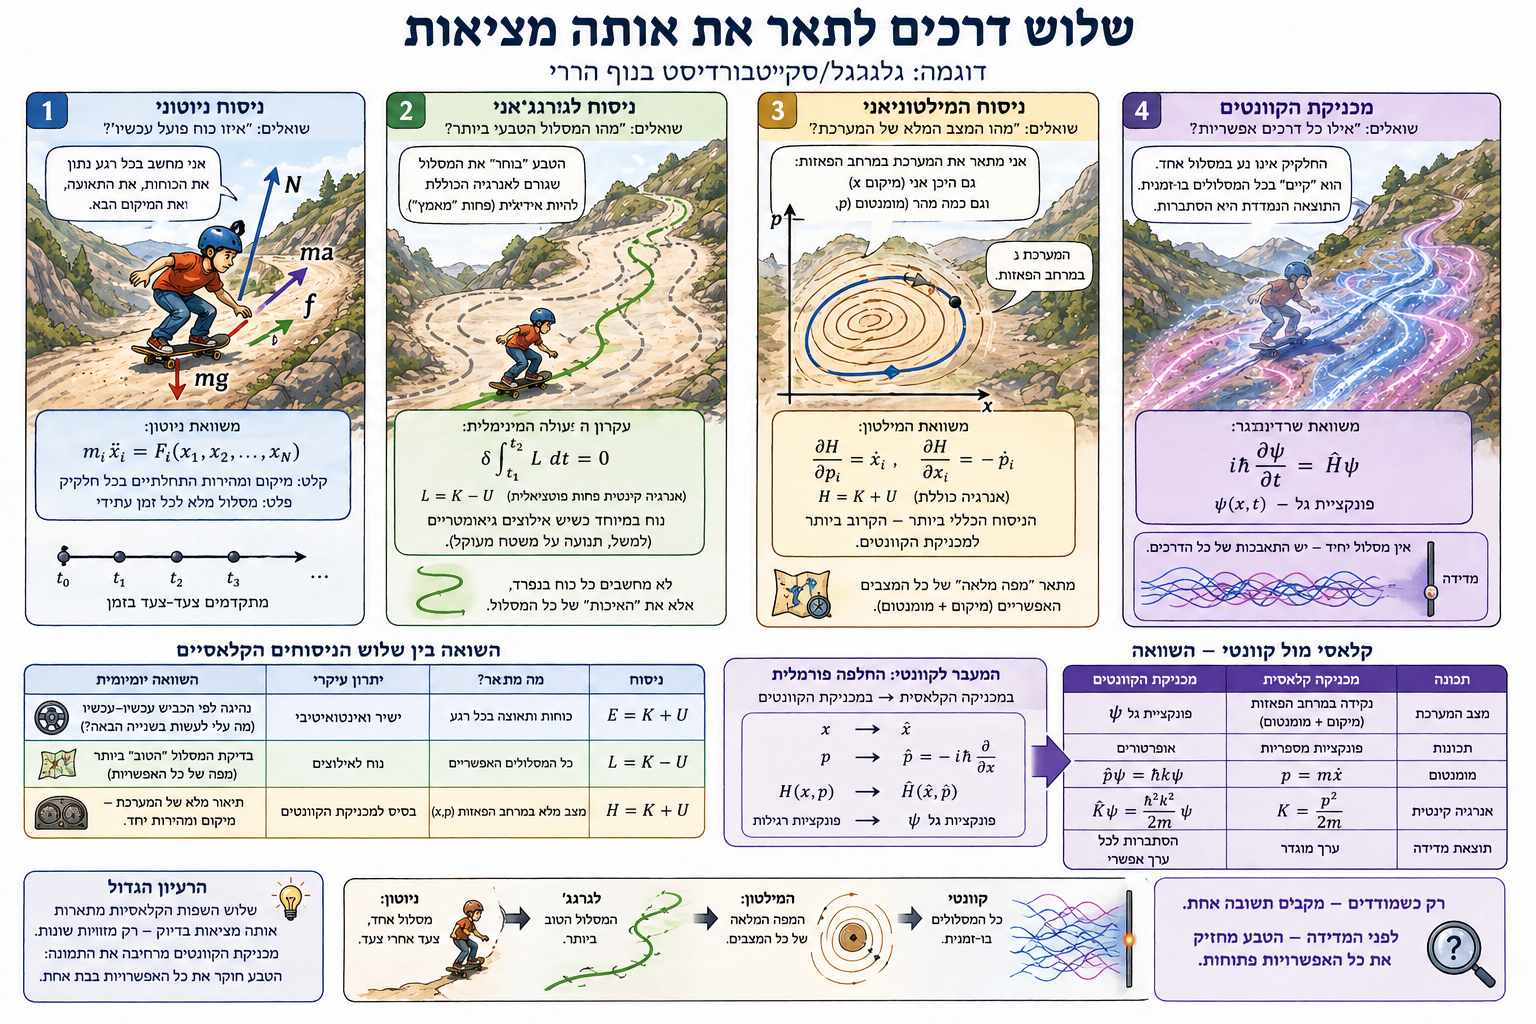
\includegraphics[keepaspectratio]{chapters/../images/image17.AnalyticalMechanics.png}}
\#\# 3.5 משוואת שרדינגר --- לב המכניקה הקוונטית

\subsection{הערה חשובה לפני
הגזירה}\label{ux5d4ux5e2ux5e8ux5d4-ux5d7ux5e9ux5d5ux5d1ux5d4-ux5dcux5e4ux5e0ux5d9-ux5d4ux5d2ux5d6ux5d9ux5e8ux5d4}

\textbf{לא ניתן לגזור את משוואת שרדינגר} מעקרונות פשוטים יותר --- היא
\textbf{פוסטולט}. מה שמוצג כאן הוא \textbf{פיתוח היוריסטי} (heuristic)
--- טיעון מונחה-תוצאה שמראה \emph{איך אפשר היה להגיע אליה}, לא
\emph{הוכחה} שהיא נכונה. הסיבה שמקבלים אותה: היא עובדת. כל ניסוי שנעשה
אישר אותה.

\subsection{הפיתוח}\label{ux5d4ux5e4ux5d9ux5eaux5d5ux5d7}

\textbf{שלב 1 --- שימור אנרגיה:}

\[E = \frac{p^2}{2m} + U(\mathbf{r}, t)\]

אנרגיה כוללת = קינטית + פוטנציאלית. זה קלאסי לחלוטין.

\textbf{שלב 2 --- תיאור גלי:}

לפי פוסטולט הדואליות, לכל חלקיק יש פונקציית גל. עבור חלקיק חופשי (ללא
פוטנציאל):

\[\psi(\mathbf{r},t) = C e^{i(\mathbf{k}\cdot\mathbf{r} - \omega t)}\]

\textbf{שלב 3 --- יחסי פלנק-איינשטיין-דה-ברויי:}

\[E = \hbar\omega, \qquad p = \hbar k\]

\textbf{שלב 4 --- חיבור הכל:}

מציבים יחסים אלו בשימור האנרגיה ומכפילים ב-\(\psi\):

\[\hbar\omega\psi = \frac{\hbar^2 k^2}{2m}\psi + U\psi\]

\textbf{שלב 5 --- מעבר לאופרטורים:}

בניסוח המילטוניאני, אנרגיה מתאימה לנגזרת בזמן ומומנטום --- לנגזרת במרחב.
לאחר החלפה:

\[\boxed{i\hbar\frac{\partial\psi(\mathbf{r},t)}{\partial t} = -\frac{\hbar^2}{2m}\nabla^2\psi(\mathbf{r},t) + U(\mathbf{r})\psi(\mathbf{r},t)}\]

זוהי \textbf{משוואת שרדינגר התלויה בזמן}.

\subsection{קריאת
המשוואה}\label{ux5e7ux5e8ux5d9ux5d0ux5ea-ux5d4ux5deux5e9ux5d5ux5d5ux5d0ux5d4}

הצד השמאלי: \(i\hbar\frac{\partial\psi}{\partial t}\) --- שינוי פונקציית
הגל בזמן, כפול קבוע. זה ``מה שקורה''.

הצד הימני: \(-\frac{\hbar^2}{2m}\nabla^2\psi + U\psi\) --- האנרגיה
הקינטית + האנרגיה הפוטנציאלית, פועלות כאופרטורים על \(\psi\). זה
``הכוחות הפועלים''.

\(\nabla^2 = \frac{\partial^2}{\partial x^2} + \frac{\partial^2}{\partial y^2} + \frac{\partial^2}{\partial z^2}\)
הוא \textbf{האופרטור לפלסיאן} --- נגזרת שנייה בכל שלושת הכיוונים.

הצד הימני כולו הוא למעשה \textbf{האופרטור המילטוניאני} \(\hat{H}\) הפועל
על \(\psi\), ולכן המשוואה לעיתים כתובה בקצרה:
\(i\hbar\frac{\partial\psi}{\partial t} = \hat{H}\psi\).

\subsection{גרסה בלתי-תלויה
בזמן}\label{ux5d2ux5e8ux5e1ux5d4-ux5d1ux5dcux5eaux5d9-ux5eaux5dcux5d5ux5d9ux5d4-ux5d1ux5d6ux5deux5df}

עבור מערכות שאינן משתנות בזמן (פוטנציאל קבוע), פונקציית הגל מתפרדת לשני
גורמים: \(\Psi(x,t)=\psi(x)\cdot\phi(t)\), כאשר החלק התלוי בזמן הוא
\(\psi(t) = e^{−\frac{iEt}{\hbar}}\). גורם זה אינו נעלם, אך מתבטל כאשר
מחשבים ערכים נצפים, מכיוון שב-\(|\Psi|^2\) האקספוננטות מתבטלות זו עם זו.
לכן, עבור מצבים מתמידים, עובדים רק עם
ψ(x)\hspace{0pt}\hspace{0pt}\hspace{0pt}\hspace{0pt}\hspace{0pt}\hspace{0pt}\hspace{0pt}\hspace{0pt}\hspace{0pt}\hspace{0pt}\hspace{0pt}\hspace{0pt}
ומקבלים:

\[\hat{H}\psi = E\psi\]

זוהי \textbf{משוואת הערכים העצמיים של האנרגיה} --- פונקציות עצמיות של
\(\hat{H}\) הן מצבי האנרגיה המוגדרים, והערכים העצמיים \(E\) הם האנרגיות
האפשריות. רמות האנרגיה הדיסקרטיות של האטום --- שגרמו לקווים הספקטרליים
--- יוצאות ממשוואה זו. ואם היינו מתחילים ממשוואת שרדינגר התלויה בזמן, אז
במהלך הפתרון עדיין היינו מגיעים לביטול של החלק התלוי בזמן של פונקציית
הגל ולרמות אנרגיה. וזה למעשה משמש כהוכחה מתמטית של יציבות הרמות
הסטציונריות בנוסח של אטום בור, ואף של יציבות האטום בכלל.

\pandocbounded{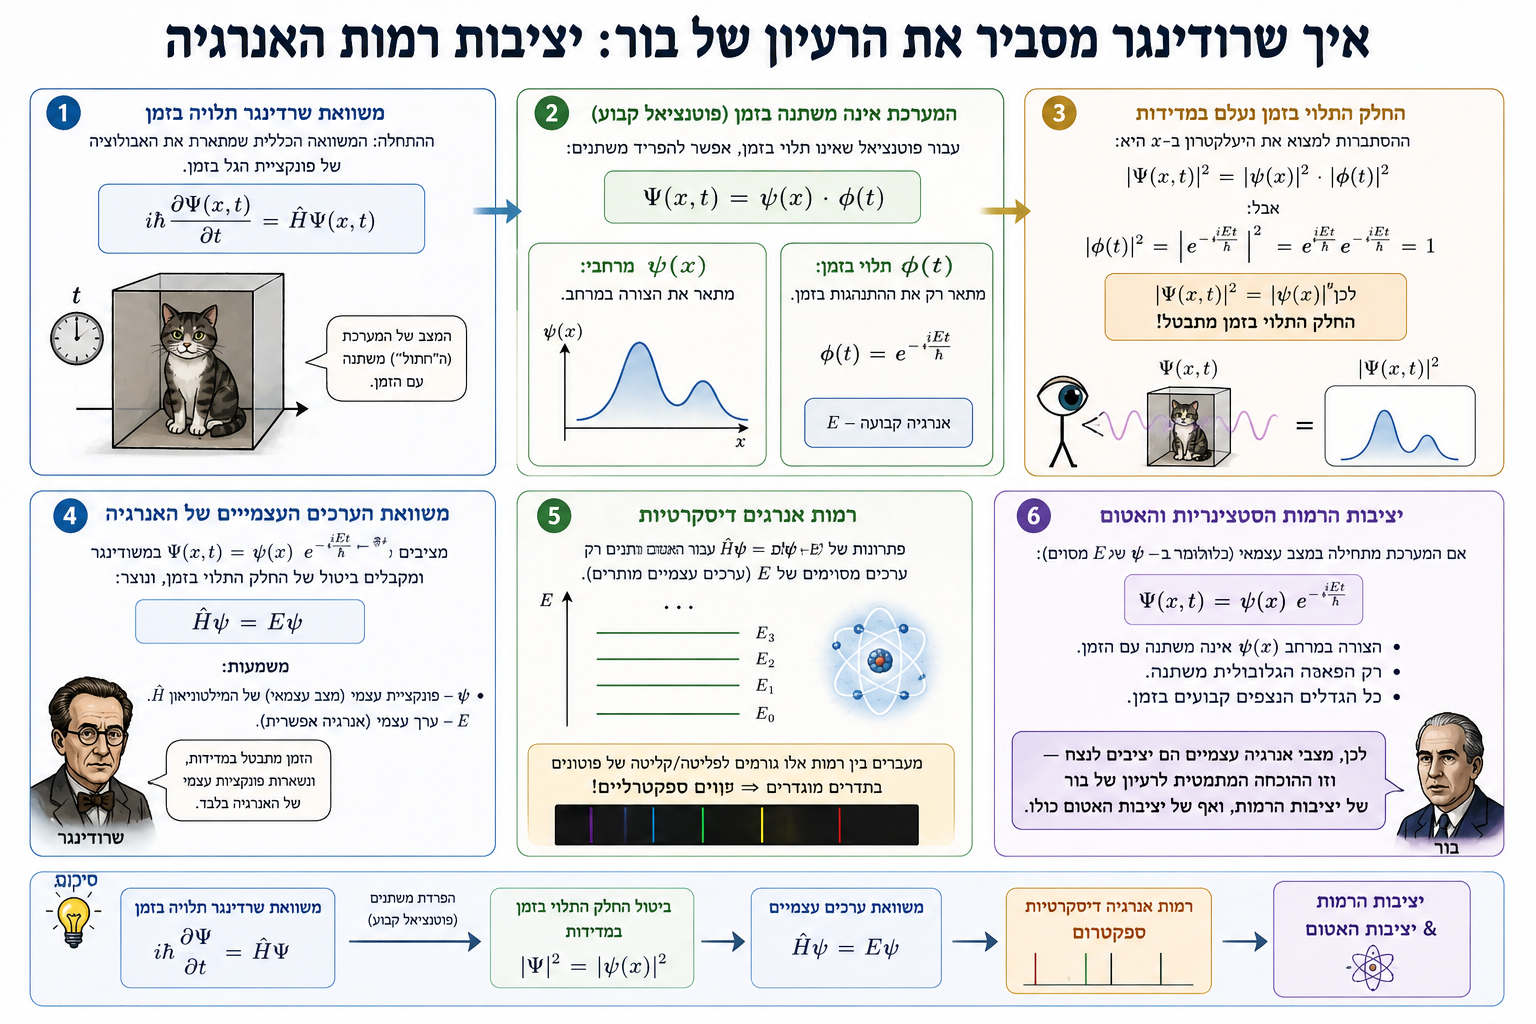
\includegraphics[keepaspectratio]{chapters/../images/image18.SchroedingerAndBohr.png}}
\#\# 3.6 פתרון לאטום המימן --- אורביטלים ומספרים קוונטיים

\subsection{מהי הבעיה?}\label{ux5deux5d4ux5d9-ux5d4ux5d1ux5e2ux5d9ux5d4}

אטום המימן הוא מערכת של גרעין ואלקטרון אחד. הפוטנציאל הוא כוח קולומב:

\[U = -\frac{e^2}{4\pi\varepsilon_0 r}\]

כאשר \(r\) הוא המרחק בין האלקטרון לגרעין. זוהי בעיית \textbf{שני גופים}
שניתן להפחיתה לבעיית \textbf{גוף אחד} בקואורדינטות כדוריות
\((r, \theta, \varphi)\).

\subsection{הפתרון}\label{ux5d4ux5e4ux5eaux5e8ux5d5ux5df}

פונקציות הגל של אטום המימן הן מהצורה:

\[\Psi_{n,l,m}(r,\theta,\varphi) = R_{n,l}(r) \cdot \Theta_{l,m}(\theta) \cdot \Phi_m(\varphi)\]

שלושה גורמים: רדיאלי, קוטבי ואזימוטלי. \textbf{מתנאי הרציפות} של כל גורם
נובע שהפתרונות קיימים רק עבור \textbf{מספרים שלמים ספציפיים} --- וכך
מגיעים ל\textbf{מספרים הקוונטיים}.

\subsection{הערה חשובה: ``רק
למימן''?}\label{ux5d4ux5e2ux5e8ux5d4-ux5d7ux5e9ux5d5ux5d1ux5d4-ux5e8ux5e7-ux5dcux5deux5d9ux5deux5df}

נפוץ לשמוע שמשוואת שרדינגר ניתנת לפתרון \textbf{אנליטי} רק לאטום המימן.
זה נכון --- אבל מטעה.

\begin{itemize}
\tightlist
\item
  \textbf{פתרון אנליטי}: מניפולציות אלגבריות עד נוסחה סגורה. אפשרי רק
  לחד-אלקטרוניים.
\item
  \textbf{פתרון נומרי}: הצבת ערכים ובדיקה. \textbf{אפשרי לכל אטום},
  בדיוק כל שרוצים, תלוי בזמן חישוב.
\end{itemize}

יתרה מזו: לא רק מימן --- גם \(\text{He}^+\), \(\text{Li}^{2+}\), ואפילו
\(\text{Fe}^{25+}\) ניתנים לפתרון \textbf{אנליטי}, כי כולם מערכות
חד-אלקטרוניות. אטומים רב-אלקטרוניים מורכבים יותר כי האלקטרונים דוחים זה
את זה --- אבל גם הם פתירים נומרית. \#\# 3.7 ארבעת המספרים הקוונטיים

מפתרון משוואת שרדינגר לאטום המימן, מופיעים שלושה מספרים שלמים בהכרח.
ספין נוסף כמספר רביעי מאוחר יותר.
\pandocbounded{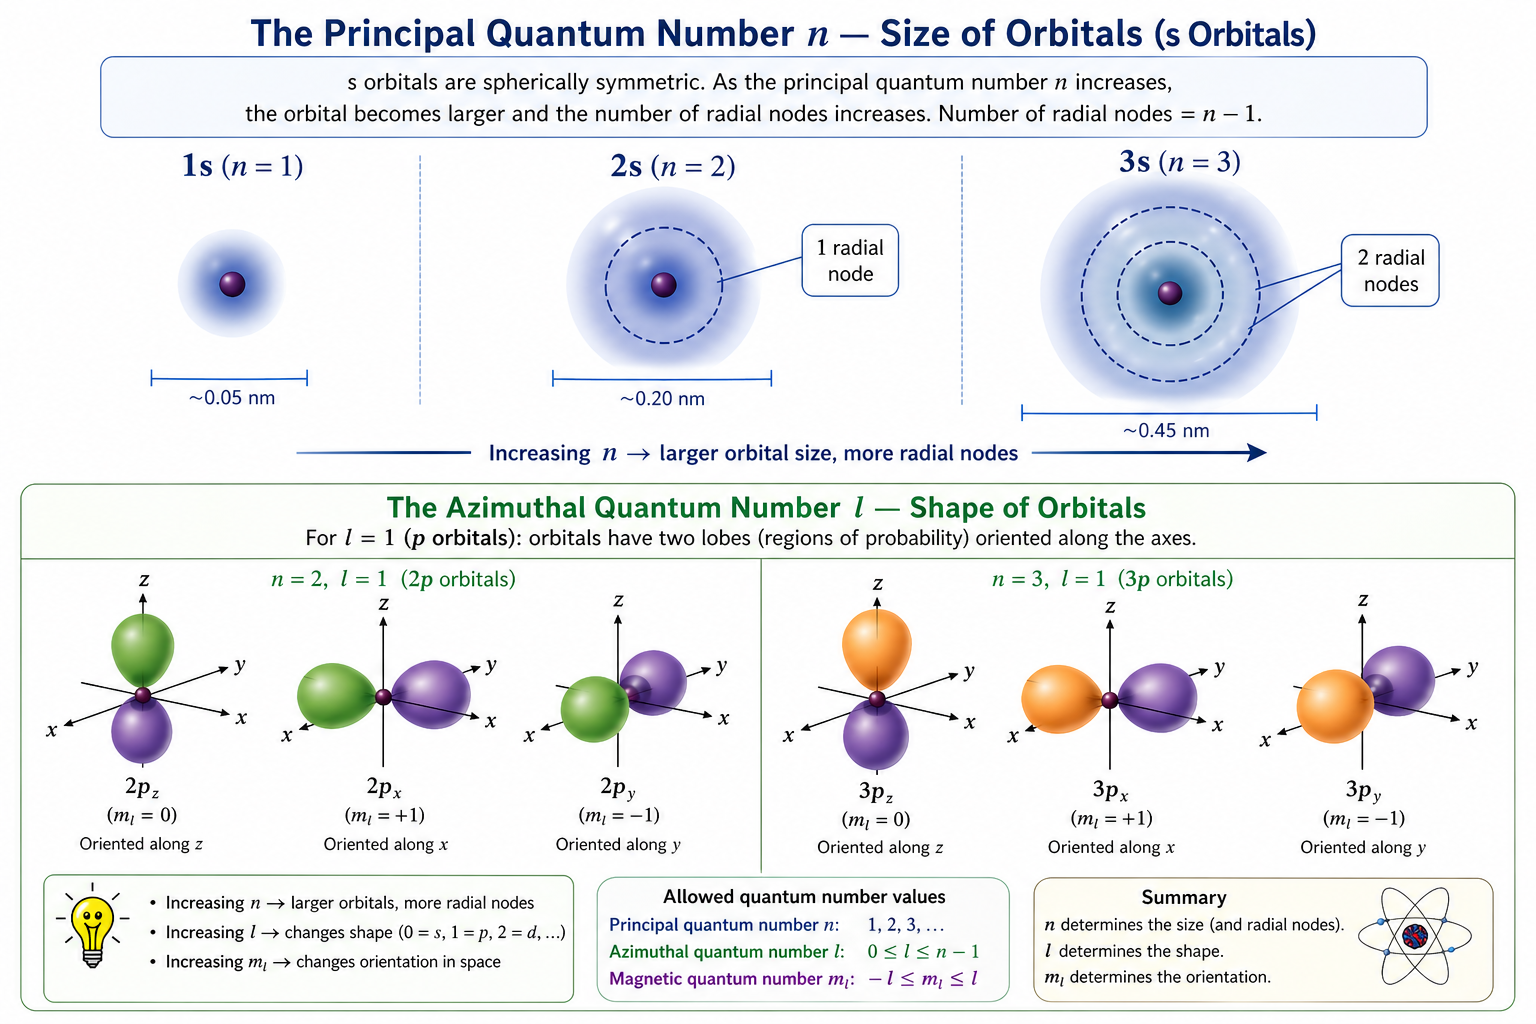
\includegraphics[keepaspectratio,alt={image19.quantumNumbers.png}]{chapters/../images/image19.quantumNumbers.png}}
\#\#\# \(n\) --- מספר קוונטי ראשי (Principal quantum number)

\[n = 1, 2, 3, \ldots\]

קובע את \textbf{רמת האנרגיה הכוללת} ואת \textbf{הרדיוס הממוצע} מהגרעין.
\(n=1\) --- הרמה הנמוכה ביותר (הפנימית). לאטום מימן:

\[E_n = -\frac{13.6\ \text{eV}}{n^2}\]

\subsection{\texorpdfstring{\(l\) --- מספר קוונטי אורביטלי (Orbital /
Angular momentum quantum
number)}{l --- מספר קוונטי אורביטלי (Orbital / Angular momentum quantum number)}}\label{l-ux5deux5e1ux5e4ux5e8-ux5e7ux5d5ux5d5ux5e0ux5d8ux5d9-ux5d0ux5d5ux5e8ux5d1ux5d9ux5d8ux5dcux5d9-orbital-angular-momentum-quantum-number}

\[l = 0, 1, 2, \ldots, (n-1)\]

קובע את \textbf{צורת האורביטל} --- בעצם, את מספר נקודות הקיצון של
פונקציית הגל. לכל ערך יש שם:

{\def\LTcaptype{none} % do not increment counter
\begin{longtable}[]{@{}lllll@{}}
\toprule\noalign{}
\(l\) & 0 & 1 & 2 & 3 \\
\midrule\noalign{}
\endhead
\bottomrule\noalign{}
\endlastfoot
שם & s & p & d & f \\
\end{longtable}
}

\begin{itemize}
\tightlist
\item
  \(l=0\) (s): \textbf{אורביטל כדורי} --- ללא כיוון מועדף, סימטרי
\item
  \(l=1\) (p): \textbf{אורביטל דמוי שמינייה} --- יש כיוון מועדף, שלושה
  אורביטלים שונים בכיוון
\item
  \(l=2\) (d): \textbf{אורביטלים מורכבים יותר} --- חמישה אורביטלים
\end{itemize}

\subsection{\texorpdfstring{\(m_l\) --- מספר קוונטי מגנטי (Magnetic
quantum
number)}{m\_l --- מספר קוונטי מגנטי (Magnetic quantum number)}}\label{m_l-ux5deux5e1ux5e4ux5e8-ux5e7ux5d5ux5d5ux5e0ux5d8ux5d9-ux5deux5d2ux5e0ux5d8ux5d9-magnetic-quantum-number}

\[m_l = -l, -(l-1), \ldots, 0, \ldots, (l-1), l\]

קובע את \textbf{כיוון האורביטל במרחב} --- היטל המומנט הזוויתי על ציר
קבוע. לכל \(l\) יש \((2l+1)\) ערכים, כלומר \((2l+1)\) אורביטלים שונים
בכיוון.

\begin{quote}
\textbf{הערה:} אין התאמה ``טבעית'' בין הערך המספרי של \(m_l\) לצורה
ספציפית. ההקצאה שרירותית --- מה שנקבע הוא רק \textbf{כמה} אורביטלים:
\(l=1\) נותן שלושה, \(l=2\) נותן חמישה.
\end{quote}

\subsection{\texorpdfstring{\(m_s\) --- ספין (Spin quantum
number)}{m\_s --- ספין (Spin quantum number)}}\label{m_s-ux5e1ux5e4ux5d9ux5df-spin-quantum-number}

\[m_s = +\frac{1}{2} \quad \text{או} \quad -\frac{1}{2}\]

הספין אינו נובע ממשוואת שרדינגר --- הוא \textbf{תכונה מהותית} של
האלקטרון (ושל כל פרמיון). לאלקטרון יש בדיוק שני ערכים: ``ספין מעלה''
ו''ספין מטה''. בפועל כותבים \(\pm\frac{1}{2}\) כאשר \(\hbar\) נלקח כמובן
מאליו.

\subsection{ספירת
אורביטלים}\label{ux5e1ux5e4ux5d9ux5e8ux5ea-ux5d0ux5d5ux5e8ux5d1ux5d9ux5d8ux5dcux5d9ux5dd}

{\def\LTcaptype{none} % do not increment counter
\begin{longtable}[]{@{}llll@{}}
\toprule\noalign{}
\(n\) & \(l\) אפשריים & \(m_l\) לכל \(l\) & סה''כ אורביטלים \\
\midrule\noalign{}
\endhead
\bottomrule\noalign{}
\endlastfoot
1 & 0 & \{0\} & 1 \\
2 & 0, 1 & \{0\}, \{-1,0,1\} & 1+3 = 4 \\
3 & 0, 1, 2 & \{0\}, \{-1,0,1\}, \{-2,-1,0,1,2\} & 1+3+5 = 9 \\
\end{longtable}
}

\textbf{כלל:} לרמה \(n\) יש \(n^2\) אורביטלים, ועם ספין --- \(2n^2\)
אלקטרונים לכל היותר. \#\# 3.8 עקרון אי-הוודאות של היזנברג

\subsection{הניסוח}\label{ux5d4ux5e0ux5d9ux5e1ux5d5ux5d7}

\[\Delta x \cdot \Delta p \geq \frac{\hbar}{2}\]

כאשר \(\Delta x\) --- אי-הוודאות במיקום, \(\Delta p\) --- אי-הוודאות
במומנטום, \(\hbar = h/2\pi \approx 1.05\times10^{-34}\ \text{J·s}\).

הוא \textbf{קבוע הסקאלה הקוונטית} --- גורם ההמרה בין הקנה הקוונטי לקנה
האנושי. כל ביטוי הנוגע לעולם הקוונטי מכיל \(\hbar\) (על כן לפעמים מדלגים
על כתיבה מפורשת של \(\hbar\)).

\subsection{מה זה אומר
בפועל?}\label{ux5deux5d4-ux5d6ux5d4-ux5d0ux5d5ux5deux5e8-ux5d1ux5e4ux5d5ux5e2ux5dc}

המכפלה \(\Delta x \cdot \Delta p\) אינה יכולה להחות קטנה מ-\(\hbar/2\).
שיפור הדיוק במיקום בא על חשבון הורדת הדיוק במומנטום --- ולהיפך.

\textbf{הקיצונות:}

\begin{itemize}
\tightlist
\item
  מיקום מדויק לחלוטין → מומנטום לגמרי לא ידוע. השלכה: לא ניתן לקבוע איך
  ולאן זז האלקטרון הנמצא בעמדה מסוימת.
\item
  מומנטום מדויק לחלוטין → מיקום לגמרי לא ידוע. השלכה: האלקטרון שתנועתו
  ידועה, יכול להיות בכל מקום ביקום.
  \pandocbounded{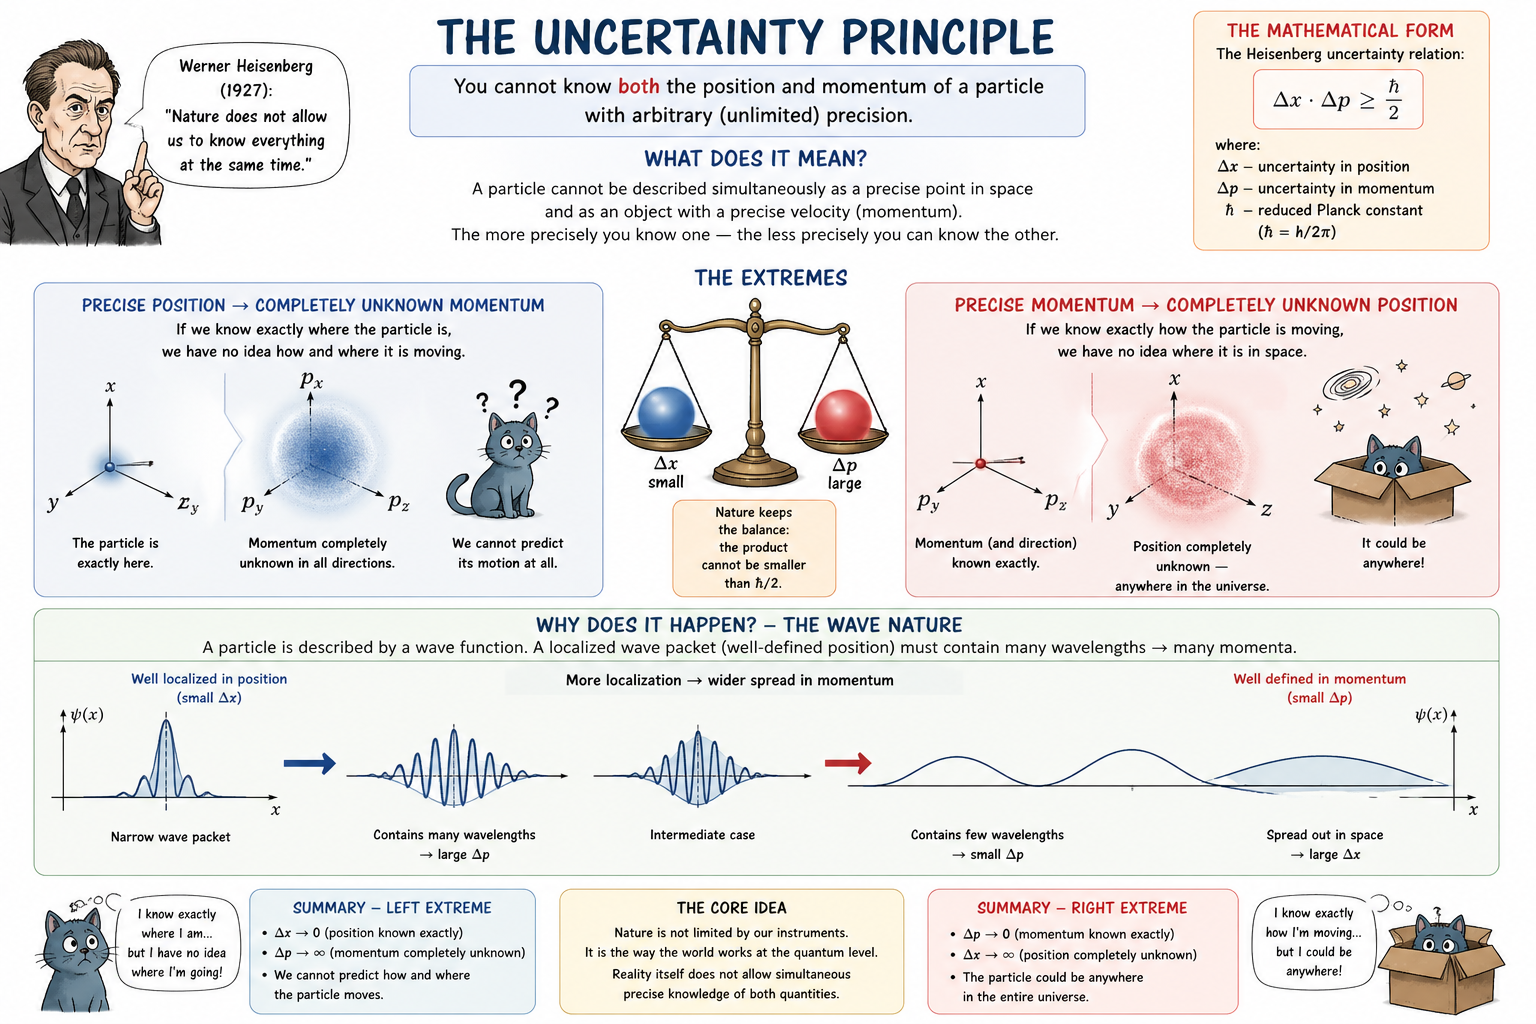
\includegraphics[keepaspectratio]{chapters/../images/image20.Heisenberg.png}}
  \#\#\# זאת לא מגבלה אן בעיה של מכשירים
\end{itemize}

חשוב להבין: עקרון אי-הוודאות \textbf{אינו} אומר שהמכשירים שלנו לא מספיק
מדויקים. הוא אומר שלאלקטרון אין בו-זמנית מיקום ומומנטום מוגדרים --- זהו
מצב פיזיקלי אמיתי, לא חוסר ידע טכני.

לכן תמונות של אטומים תמיד ``מטושטשות'' --- לא כשל של המיקרוסקופ, אלא
עובדה עקרונית.

\subsection{בקנה מידה
יומיומי}\label{ux5d1ux5e7ux5e0ux5d4-ux5deux5d9ux5d3ux5d4-ux5d9ux5d5ux5deux5d9ux5d5ux5deux5d9}

לשולחן שעורעו מטר אחד, \(\hbar\) כה קטן שאי-הוודאות במיקום היא
\(\sim 10^{-34}\ \text{m}\) שזה לא ניתן לזיהוי באף שיטת מדידה קיימת. לכן
העיקרון \textbf{איננו מורגש} בחיי יומיום.

\subsection{עקרון כללי
יותר}\label{ux5e2ux5e7ux5e8ux5d5ux5df-ux5dbux5dcux5dcux5d9-ux5d9ux5d5ux5eaux5e8}

עקרון אי-הוודאות חל על כל \textbf{זוג תכונות שאינן ``מתחלפות''} מתמטית.
זוגות חשובים:

\[\Delta x \cdot \Delta p \geq \frac{\hbar}{2}\]
\[\Delta E \cdot \Delta t \geq \frac{\hbar}{2}\]
\[\Delta L_x \cdot \Delta L_y \geq \frac{\hbar}{2}\]

הזוג \(\Delta E \cdot \Delta t\) חשוב במיוחד: מצב אנרגטי קצר-חיים
(\(\Delta t\) קטן) בהכרח בעל \textbf{רוחב ספקטרלי} גדול (\(\Delta E\)
גדול) --- ולכן הקו בספקטרום אינו חד אלא רחב. זה מסביר את \textbf{רוחב
הקווים הספקטרליים} שנצפה בניסוי. \#\# סיכום

שלושה דברים עיקריים מהפרק:

\textbf{ראשית} --- מכניקת הקוונטים אינה ``תיקון'' לפיזיקה קלאסית, אלא
השקפת עולם אחרת לחלוטין. תכונות הן אופרטורים; מצבים הם פונקציות גל;
תוצאות מדידה הן הסתברויות.

\textbf{שנית} --- משוואת שרדינגר היא לב התיאוריה. פתרונה לאטום המימן
מניב אורביטלים ומספרים קוונטיים --- ה-\(n\), \(l\), \(m_l\) יוצאים
מהמתמטיקה, לא מוכנסים ידנית.

\textbf{שלישית} --- עקרון אי-הוודאות אינו מגבלה טכנית. הוא עובדה
פיזיקלית: לאלקטרון אין בו-זמנית מיקום ומומנטום מוגדרים --- ומכאן נובעת
כל ``מטושטשות'' העולם הקוונטי.

\bookmarksetup{startatroot}

\chapter{פרק 4 --- מהאטום לטבלה המחזורית: ספין, עקרון פאולי וטרמים
אטומיים}\label{ux5e4ux5e8ux5e7-4-ux5deux5d4ux5d0ux5d8ux5d5ux5dd-ux5dcux5d8ux5d1ux5dcux5d4-ux5d4ux5deux5d7ux5d6ux5d5ux5e8ux5d9ux5ea-ux5e1ux5e4ux5d9ux5df-ux5e2ux5e7ux5e8ux5d5ux5df-ux5e4ux5d0ux5d5ux5dcux5d9-ux5d5ux5d8ux5e8ux5deux5d9ux5dd-ux5d0ux5d8ux5d5ux5deux5d9ux5d9ux5dd}

\section{מבוא: מה קובע את תכונות
היסוד?}\label{ux5deux5d1ux5d5ux5d0-ux5deux5d4-ux5e7ux5d5ux5d1ux5e2-ux5d0ux5ea-ux5eaux5dbux5d5ux5e0ux5d5ux5ea-ux5d4ux5d9ux5e1ux5d5ux5d3}

בפרק הקודם למדנו שמצב האלקטרון באטום מוגדר על ידי ארבעה מספרים קוונטיים.
אבל עדיין לא ענינו על השאלה המרכזית: \textbf{למה הטבלה המחזורית נראית
כמו שהיא נראית?} למה בשורה הראשונה יש שני יסודות, בשנייה --- שמונה, ולמה
מתכות המעבר מגיעות דווקא שם?

התשובה נובעת מהדרך שבה אלקטרונים \textbf{מאכלסים} אורביטלים, ושני כללים
שולטים בתהליך: \textbf{עקרון פאולי} וכלל \textbf{הונד}. פרק זה יציג
אותם, יסביר את הטבלה המחזורית, ויציג כלי נוסף לתיאור מצבים אטומיים ---
\textbf{הטרם האטומי}. \#\# 4.1 עקרון האי-הכלה של פאולי

\subsection{הניסוח}\label{ux5d4ux5e0ux5d9ux5e1ux5d5ux5d7-1}

\textbf{עקרון פאולי} (Wolfgang Pauli, 1925): \textbf{שני אלקטרונים באותו
אטום (ובאותה מערכת קוונטית בכלל) אינם יכולים לשאת את אותם ארבעה מספרים
קוונטיים.}

כלומר: לכל אלקטרון חייבת להיות ``כתובת'' ייחודית \((n, l, m_l, m_s)\).

\subsection{מה זה אומר
בפועל?}\label{ux5deux5d4-ux5d6ux5d4-ux5d0ux5d5ux5deux5e8-ux5d1ux5e4ux5d5ux5e2ux5dc-1}

לכל אורביטל --- שמוגדר על ידי \((n, l, m_l)\) --- יש בדיוק \textbf{שני
ערכים אפשריים} של \(m_s\): \(+\frac{1}{2}\) ו-\(-\frac{1}{2}\). לכן:

\textbf{כל אורביטל מכיל לכל היותר שני אלקטרונים --- עם ספינים מנוגדים.}

זהו הכלל שכולם מכירים: ``שני אלקטרונים לאורביטל''. עקרון פאולי הוא ההסבר
--- לא כלל שרירותי, אלא תוצאה של מכניקת הקוונטים.

\subsection{למה עקרון פאולי
נכון?}\label{ux5dcux5deux5d4-ux5e2ux5e7ux5e8ux5d5ux5df-ux5e4ux5d0ux5d5ux5dcux5d9-ux5e0ux5dbux5d5ux5df}

לשאלה זו יש תשובה עמוקה: אלקטרונים הם \textbf{פרמיונים} (fermions) ---
חלקיקים עם ספין חצי-שלם. על פי \textbf{הסטטיסטיקה של פרמי-דיראק}, שני
פרמיונים זהים אינם יכולים להיות באותו מצב קוונטי. זה עקרון כללי שחל על
כל הפרמיונים --- לא רק אלקטרונים.

לעומת זאת, \textbf{בוזונים} (bosons) --- חלקיקים עם ספין שלם --- אינם
כפופים לעקרון זה. פוטונים הם בוזונים, ולכן כמה פוטונים שרוצים יכולים
להיות באותו מצב (שזה הבסיס לרעיון של לייזר). \#\# 4.2 בניית הקונפיגורציה
האלקטרונית --- עקרון האאופבאו

\subsection{הכלל}\label{ux5d4ux5dbux5dcux5dc}

בניית הקונפיגורציה האלקטרונית של אטום במצב היסוד (ground state) מתבצעת
לפי \textbf{עקרון האאופבאו} (Aufbau --- ``בניית-על'' בגרמנית): ממלאים
אורביטלים \textbf{מהאנרגיה הנמוכה ביותר כלפי מעלה}, תוך שמירה על עקרון
פאולי.

\subsection{סדר מילוי}\label{ux5e1ux5d3ux5e8-ux5deux5d9ux5dcux5d5ux5d9}

לרמות נמוכות הסדר פשוט: \(1s, 2s, 2p, 3s, 3p\). מכאן מסתבך מעט בגלל
שאנרגיית \(3d\) גבוהה מ-\(4s\), ובהמשך גם אנרגיית \(4f\) גבוהה מ-\(5s\)
ו-\(5p\):

\begin{align*}
1s \to 2s \to 2p \to 3s \to 3p \to 4s \to 3d \to 4p \to 5s &\to 4d \to 5p \to \\
&\to 6s \to 4f \to 5d \to 6p \to 7s \to 5f \to 6d \to \ldots
\end{align*}

\textbf{כלל אצבע:} אורביטל \(ns\) מתמלא לפני \((n-1)d\) ולפני
\((n-2)f\).

\subsection{דוגמאות}\label{ux5d3ux5d5ux5d2ux5deux5d0ux5d5ux5ea}

\textbf{מימן (H, \(Z=1\)):} \(1s^1\)

\textbf{הליום (He, \(Z=2\)):} \(1s^2\) --- אורביטל \(1s\) מלא. שני
אלקטרונים, ספינים מנוגדים.

\textbf{ליתיום (Li, \(Z=3\)):} \(1s^2\ 2s^1\) --- האלקטרון השלישי חייב
ללכת ל-\(2s\).

\textbf{פחמן (C, \(Z=6\)):} \(1s^2\ 2s^2\ 2p^2\) --- שני האלקטרונים
ב-\(2p\) ייפגשו עם הכלל הבא.

\textbf{נתרן (Na, \(Z=11\)):} \(1s^2\ 2s^2\ 2p^6\ 3s^1\) --- כתיב קצר:
\([\text{Ne}]\ 3s^1\).

\textbf{עופרת (Pb, \(Z=82\)):}
\([\text{Xe}]\ 4f^{14}\ 5d^{10}\ 6s^2\ 6p^2\) --- אנלוג כבד של פחמן,
אותה קונפיגורציה של \(ns^2\ np^2\).

\textbf{פראזאודימיום (Pr, \(Z=59\)):} \([\text{Xe}]\ 4f^3\ 6s^2\) ---
לנתנייד טיפוסי, תת-הרמה \(4f\) מתמלאת בהדרגה.

\textbf{זהב (Au, \(Z=79\)):} \([\text{Xe}]\ 4f^{14}\ 5d^{10}\ 6s^1\) ---
יוצא דופן: האלקטרון האחד עובר מ-\(6s^2\) ל-\(5d\) כדי להשלים את תת-הרמה.

\textbf{תוריום (Th, \(Z=90\)):} \([\text{Rn}]\ 6d^2\ 5f^0\ 7s^2\) ---
בניגוד למה שהיה מצופה, שני האלקטרונים הראשונים של האקטינידים נכנסים
ל-\(6d\) ולא ל-\(5f\).

\textbf{כלל הונד הראשון} (Friedrich Hund, 1927): \textbf{כאשר ממלאים
אורביטלים בעלי אנרגיה שווה, ממקמים אלקטרון אחד בכל אורביטל לפני שמוסיפים
אלקטרון שני לאורביטל כלשהו --- וכל האלקטרונים הבודדים בעלי ספין מקביל.}

\textbf{למה?} שני אלקטרונים באורביטלים שונים נמצאים בממוצע רחוקים יותר
זה מזה --- ולכן האנרגיה האלקטרוסטטית (הדחייה) קטנה יותר. המצב עם יותר
ספינים מקבילים יציב יותר.

\subsection{\texorpdfstring{דוגמה: פחמן
(\(1s^2\ 2s^2\ 2p^2\))}{דוגמה: פחמן (1s\^{}2\textbackslash{} 2s\^{}2\textbackslash{} 2p\^{}2)}}\label{ux5d3ux5d5ux5d2ux5deux5d4-ux5e4ux5d7ux5deux5df-1s2-2s2-2p2}

שלושה אורביטלי \(2p\): \(2p_x\), \(2p_y\), \(2p_z\). שני אלקטרונים למקם.

\textbf{לא נכון:} שני אלקטרונים עם ספינים מנוגדים באותו \(2p_x\).

\textbf{נכון:} אלקטרון אחד ב-\(2p_x\) ואחד ב-\(2p_y\), \textbf{שניהם עם
ספין מעלה}.

ציור תאים קוונטיים לפחמן:

\[2p: \quad \boxed{\uparrow} \quad \boxed{\uparrow} \quad \boxed{\phantom{\uparrow}}\]

\subsection{\texorpdfstring{דוגמה: חמצן
(\(1s^2\ 2s^2\ 2p^4\))}{דוגמה: חמצן (1s\^{}2\textbackslash{} 2s\^{}2\textbackslash{} 2p\^{}4)}}\label{ux5d3ux5d5ux5d2ux5deux5d4-ux5d7ux5deux5e6ux5df-1s2-2s2-2p4}

ארבעה אלקטרונים ב-\(2p\):

\[2p: \quad \boxed{\uparrow\downarrow} \quad \boxed{\uparrow} \quad \boxed{\uparrow}\]
\#\# 4.4 הטבלה המחזורית --- הכל נובע ממספרים קוונטיים

\subsection{השורות}\label{ux5d4ux5e9ux5d5ux5e8ux5d5ux5ea}

{\def\LTcaptype{none} % do not increment counter
\begin{longtable}[]{@{}
  >{\raggedright\arraybackslash}p{(\linewidth - 6\tabcolsep) * \real{0.0588}}
  >{\raggedright\arraybackslash}p{(\linewidth - 6\tabcolsep) * \real{0.3235}}
  >{\raggedright\arraybackslash}p{(\linewidth - 6\tabcolsep) * \real{0.1618}}
  >{\raggedright\arraybackslash}p{(\linewidth - 6\tabcolsep) * \real{0.4559}}@{}}
\toprule\noalign{}
\begin{minipage}[b]{\linewidth}\raggedright
שורה
\end{minipage} & \begin{minipage}[b]{\linewidth}\raggedright
תת-רמות מתמלאות
\end{minipage} & \begin{minipage}[b]{\linewidth}\raggedright
מספר יסודות
\end{minipage} & \begin{minipage}[b]{\linewidth}\raggedright
הסבר
\end{minipage} \\
\midrule\noalign{}
\endhead
\bottomrule\noalign{}
\endlastfoot
1 & \(1s\) & 2 & אורביטל \(1s\) אחד, 2 אלקטרונים \\
2 & \(2s\), \(2p\) & 8 & \(2s\) (2) + \(2p\) (6) \\
3 & \(3s\), \(3p\) & 8 & \(3s\) (2) + \(3p\) (6) \\
4 & \(4s\), \(3d\), \(4p\) & 18 & \(4s\) (2) + \(3d\) (10) + \(4p\)
(6) \\
5 & \(5s\), \(4d\), \(5p\) & 18 & כנ''ל \\
6 & \(6s\), \(4f\), \(5d\), \(6p\) & 32 & כנ''ל + \(4f\) (14) \\
\end{longtable}
}

\subsection{הגושים
בטבלה}\label{ux5d4ux5d2ux5d5ux5e9ux5d9ux5dd-ux5d1ux5d8ux5d1ux5dcux5d4}

\textbf{גוש s} (עמודות 1-2): מתמלאים אורביטלי \(s\).

\textbf{גוש p} (עמודות 13-18): מתמלאים אורביטלי \(p\).

\textbf{גוש d} (מתכות מעבר, עמודות 3-12): מתמלאים אורביטלי \(d\).

\textbf{גוש f} (לנתנידים ואקטינידים): מתמלאים אורביטלי \(f\).

\subsection{מתכות מעבר --- למה הן
מיוחדות?}\label{ux5deux5eaux5dbux5d5ux5ea-ux5deux5e2ux5d1ux5e8-ux5dcux5deux5d4-ux5d4ux5df-ux5deux5d9ux5d5ux5d7ux5d3ux5d5ux5ea}

מתכות מעבר הן יסודות שבהם מתמלאים אורביטלי \(3d\) (או \(4d\), \(5d\)).
האורביטלים \(d\) בעלי \textbf{חמישה} אורביטלים עם \textbf{עשרה}
אלקטרונים אפשריים --- לכן יש עשר מתכות מעבר בכל שורה.

מתכות מעבר מעניינות כי אורביטלי \(d\) חלקית מלאים --- מה שגורם לתכונות
מגנטיות, ריבוי מצבי חמצון, וצבעים שונים (שנסביר בהמשך הקורס).

\subsection{``חריגים''
בקונפיגורציה}\label{ux5d7ux5e8ux5d9ux5d2ux5d9ux5dd-ux5d1ux5e7ux5d5ux5e0ux5e4ux5d9ux5d2ux5d5ux5e8ux5e6ux5d9ux5d4}

כמה יסודות ``מפתיעים'' לכאורה:

\textbf{כרום (Cr, \(Z=24\)):} במקום \([\text{Ar}]\ 3d^4\ 4s^2\), מה שהיה
צפוי --- בפועל: \([\text{Ar}]\ 3d^5\ 4s^1\).

\textbf{נחושת (Cu, \(Z=29\)):} במקום \([\text{Ar}]\ 3d^9\ 4s^2\) ---
בפועל: \([\text{Ar}]\ 3d^{10}\ 4s^1\).

הסיבה: תת-רמה \(d\) \textbf{מלאה לחלוטין} (\(d^{10}\)) או \textbf{מלאה
לחצי} (\(d^5\)) מייצגת יציבות מיוחדת. כדי להגיע למצב זה, ``שווה'' להעביר
אלקטרון אחד מ-\(4s\) ל-\(3d\). \#\# 4.5 טרמים אטומיים --- תיאור מדויק
יותר של מצב האטום

\subsection{מדוע צריך
טרם?}\label{ux5deux5d3ux5d5ux5e2-ux5e6ux5e8ux5d9ux5da-ux5d8ux5e8ux5dd}

הקונפיגורציה האלקטרונית (כמו \([\text{Ar}]\ 3d^3\ 4s^2\)) אינה מלאה ---
היא אינה מספרת על \textbf{כיוון} המומנטים הזוויתיים של האלקטרונים. שני
אטומים עם אותה קונפיגורציה יכולים להיות במצבים אנרגטיים שונים.

\textbf{טרם אטומי} (atomic term) הוא תיאור מדויק יותר, המציין את
\textbf{המומנטים הזוויתיים הכוללים} של כל האטום --- לא של אלקטרון בודד.

קונפיגורציה אלקטרונית מראה אילו אורביטלים תפוסים, אך אינה מתארת באופן
מלא את המצב הקוונטי של האטום. טרמים אטומיים לוקחים בחשבון את הספין הכולל
ואת המומנט המסלולי (orbit) של האלקטרונים, ולכן:

\begin{enumerate}
\def\labelenumi{\arabic{enumi}.}
\item
  קונפיגורציה אחת יכולה להתאים למספר מצבים שונים עם אנרגיות שונות.
  לדוגמה, הקונפיגורציה \(2p^2\) של פחמן נותנת שלושה טרמים: \(^3P\),
  \(^1D\) ו-\(^1S\) --- עם הפרשי אנרגיה של עשרות אלפי
  \(\text{cm}^{-1}\).
\item
  טרמים הכרחיים להבנת ספקטרים וכללי ברירה. הקווים הצהובים המפורסמים של
  נתרן (589 נ''מ) הם תוצאה של המבנה העדין של הטרם
  \(3p\ ^2P_{1/2,\ 3/2}\).
\item
  הם חשובים במיוחד לתיאור מצבים מעוררים, שבהם ריבוי הטרמים האפשריים גדל
  במהירות.
\item
  לאטומים כבדים, האינטראקצה של ספין-מסלול (אורביט \emph{l}) חזקה וזה
  מערבב טרמים שונים, וסכמת \(LS\) הפשוטה מפנה מקום לצימוד \(jj\).
  \textbf{הקונפיגורציה אומרת היכן נמצאים האלקטרונים.}
\end{enumerate}

\textbf{הטרם אומר כיצד הם באמת מקיימים אינטראקציה.}

\pandocbounded{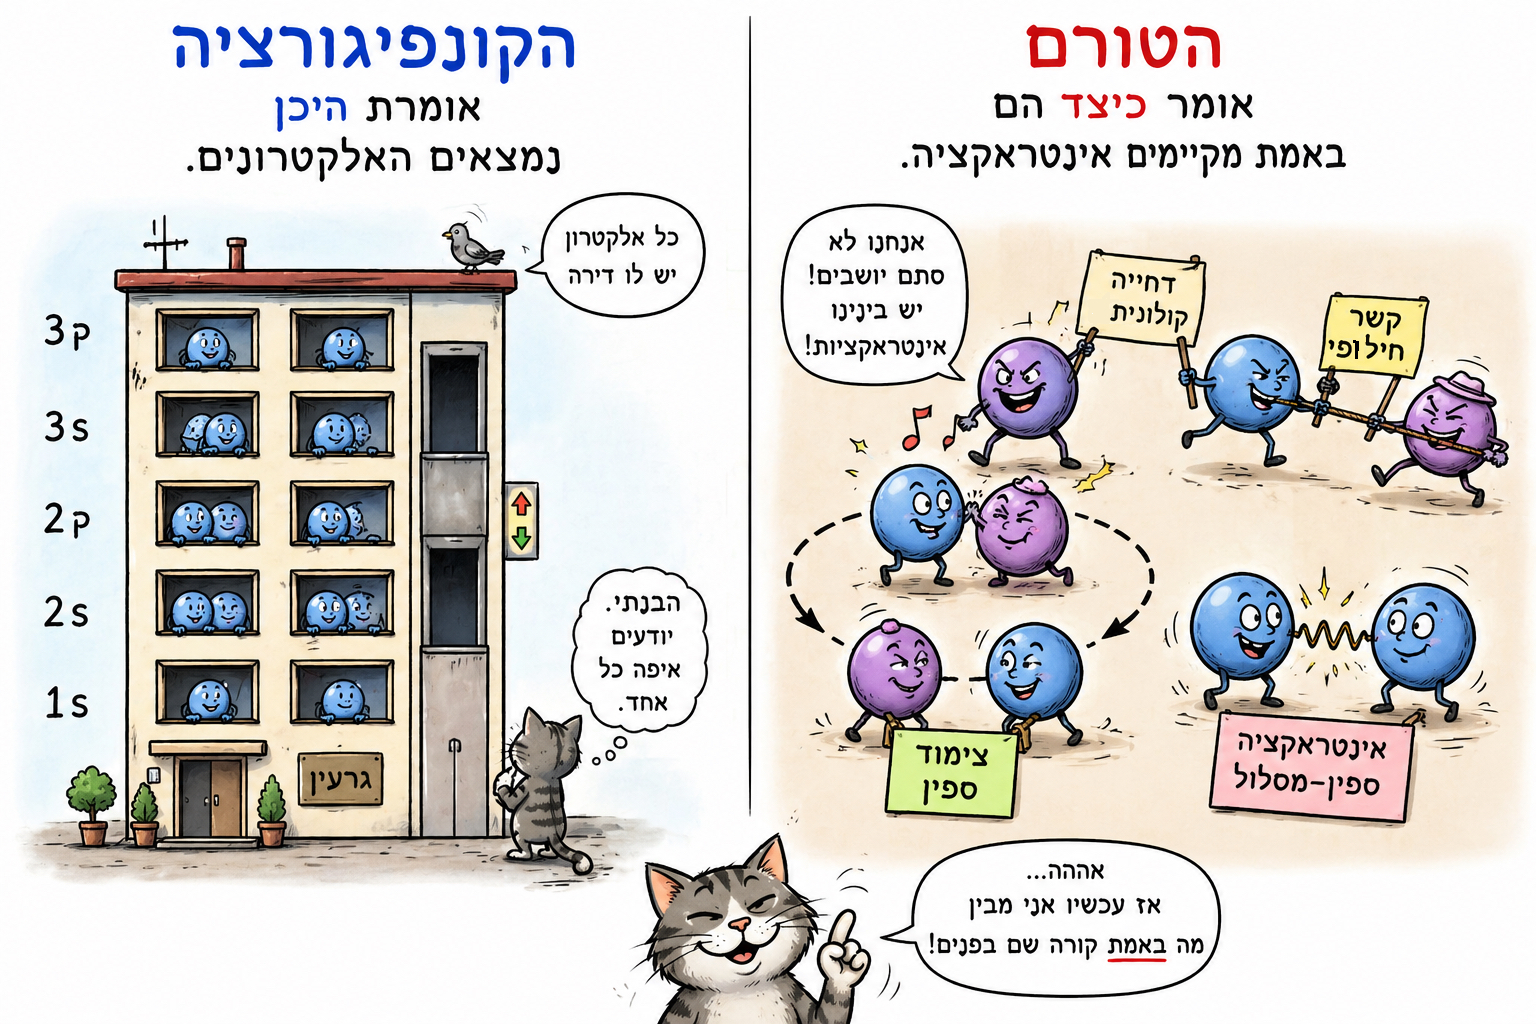
\includegraphics[keepaspectratio]{chapters/../images/image21.Terms.jpeg}}
\#\#\# שלושה גורמים --- שלושה אותיות גדולות

אנחנו מכירים \(l\) ו-\(m_s\) לאלקטרון בודד. לאטום \textbf{כולו}:

\begin{itemize}
\tightlist
\item
  \textbf{\(L\)} --- המומנט האורביטלי הכולל (סכום ה-\(m_l\) של כל
  האלקטרונים החיצוניים)
\item
  \textbf{\(S\)} --- הספין הכולל (סכום ה-\(m_s\) של כל האלקטרונים
  החיצוניים)
\item
  \textbf{\(J\)} --- המומנט הזוויתי הכולל (\(L\) ו-\(S\) מצטרפים)
\end{itemize}

\textbf{עיקרון:} אלקטרונים בשכבות \textbf{מלאות} מבטלים זה את זה לחלוטין
(\(L=0\), \(S=0\)). מחשבים רק אלקטרוני השכבה החיצונית הפתוחה.

\subsection{\texorpdfstring{חישוב
\(L\)}{חישוב L}}\label{ux5d7ux5d9ux5e9ux5d5ux5d1-l}

\[L = \left|\sum_i m_{l,i}\right| \qquad\]

כמו עם \(l\) לאלקטרון בודד, \(L\) מתורגם לאות:

{\def\LTcaptype{none} % do not increment counter
\begin{longtable}[]{@{}lllllll@{}}
\toprule\noalign{}
\(L\) & 0 & 1 & 2 & 3 & 4 & 5 \\
\midrule\noalign{}
\endhead
\bottomrule\noalign{}
\endlastfoot
אות & S & P & D & F & G & H \\
\end{longtable}
}

\textbf{שימו לב:} האות הגדולה (\(L\), \(S\), \(J\)) מציינת את הגורם עבור
\textbf{האטום כולו}; האות הקטנה (\(l\), \(s\)) --- עבור \textbf{אלקטרון
בודד}.

\subsection{\texorpdfstring{חישוב \(S\)
וריבוי}{חישוב S וריבוי}}\label{ux5d7ux5d9ux5e9ux5d5ux5d1-s-ux5d5ux5e8ux5d9ux5d1ux5d5ux5d9}

\[S = \left|\sum_i m_{s,i}\right|\]

מ-\(S\) מחשבים את \textbf{הריבוי} (multiplicity):

\[\text{multiplicity} = 2S + 1\]

{\def\LTcaptype{none} % do not increment counter
\begin{longtable}[]{@{}ll@{}}
\toprule\noalign{}
ריבוי & שם \\
\midrule\noalign{}
\endhead
\bottomrule\noalign{}
\endlastfoot
1 & סינגלט (singlet) \\
2 & דובלט (doublet) \\
3 & טריפלט (triplet) \\
4 & קוורטט (quartet) \\
\end{longtable}
}

השמות נגזרים מהמספרים הלטיניים.

\subsection{\texorpdfstring{חישוב
\(J\)}{חישוב J}}\label{ux5d7ux5d9ux5e9ux5d5ux5d1-j}

\(J\) יכול לקבל את הערכים:

\[J \in {|L-S|,\ |L-S|+1,\ \ldots,\ L+S}\]

כל ערך נפרד של \(J\) מגדיר \textbf{טרם נפרד} --- כלומר, קונפיגורציה אחת
יכולה לתת מספר טרמים.

\subsection{כתיב הטרם}\label{ux5dbux5eaux5d9ux5d1-ux5d4ux5d8ux5e8ux5dd}

\[^{(2S+1)}L_J\]

למשל \(^3F_4\) נקרא: ``אף-ארבע טריפלט''. קוראים: ריבוי (\(2S+1=3\)), אות
\(L\) (F), ומתחת \(J\) (4). אם ערך \(J\) הוא שבר, מקריאים אותו כך:
``חצי'' (1/2), ``שלושה חצאים'' (3/2) וכדומה. לדוגמה, \(^2P_{3/2}\) נקרא:
``דובלט פי שלושה חצאים''. \#\# 4.6 דוגמאות לחישוב טרמים

\subsection{\texorpdfstring{דוגמה 1: ונדיום (V) ---
\([\text{Ar}]\ 3d^3\ 4s^2\)}{דוגמה 1: ונדיום (V) --- {[}\textbackslash text\{Ar\}{]}\textbackslash{} 3d\^{}3\textbackslash{} 4s\^{}2}}\label{ux5d3ux5d5ux5d2ux5deux5d4-1-ux5d5ux5e0ux5d3ux5d9ux5d5ux5dd-v-textar-3d3-4s2}

השכבה \(4s^2\) מלאה --- מבטלת. נותרים שלושה אלקטרוני \(3d\).

ציור תאים (לפי כלל הונד --- ממלאים קודם עם ספין מעלה):

\[m_l:\ \ +2 \quad +1 \quad 0 \quad -1 \quad -2\]
\[\quad\quad\ \ \uparrow \quad\ \ \uparrow \quad \uparrow \quad\quad\quad\quad\]

\textbf{\(L\):} מקסימום \(= 2+1+0 = 3\) → \textbf{F}

\textbf{\(S\):} שלושה ספינים מעלה:
\(S = 3 \times \frac{1}{2} = \frac{3}{2}\) → ריבוי \(= 4\) (קוורטט)

\textbf{\(J\):}
\(J \in \left\{\frac{3}{2}, \frac{5}{2}, \frac{7}{2}, \frac{9}{2}\right\}\)

\textbf{טרמים אפשריים:} \(^4F_{3/2}\), \(^4F_{5/2}\), \(^4F_{7/2}\),
\(^4F_{9/2}\)

\subsection{\texorpdfstring{דוגמה 2: יון גופרית \(\text{S}^{2-}\) ---
\([\text{Ar}]\)}{דוגמה 2: יון גופרית \textbackslash text\{S\}\^{}\{2-\} --- {[}\textbackslash text\{Ar\}{]}}}\label{ux5d3ux5d5ux5d2ux5deux5d4-2-ux5d9ux5d5ux5df-ux5d2ux5d5ux5e4ux5e8ux5d9ux5ea-texts2--textar}

כל השכבות מלאות → \(L=0\), \(S=0\), ריבוי \(=1\), \(J=0\).

\textbf{טרם:} \(^1S_0\) --- המקרה הפשוט ביותר. גז אציל או יון עם תצורת
גז אציל תמיד \(^1S_0\).

\subsection{\texorpdfstring{דוגמה 3: אלומיניום (Al) ---
\([\text{Ne}]\ 3s^2\ 3p^1\)}{דוגמה 3: אלומיניום (Al) --- {[}\textbackslash text\{Ne\}{]}\textbackslash{} 3s\^{}2\textbackslash{} 3p\^{}1}}\label{ux5d3ux5d5ux5d2ux5deux5d4-3-ux5d0ux5dcux5d5ux5deux5d9ux5e0ux5d9ux5d5ux5dd-al-textne-3s2-3p1}

השכבה \(3s^2\) מלאה. נותר אלקטרון אחד ב-\(3p\): \(l=1\),
\(m_s=+\frac{1}{2}\).

\(L=1\) → \textbf{P}; \(S=\frac{1}{2}\) → ריבוי \(=2\) (דובלט);
\(J \in \left\{\frac{1}{2}, \frac{3}{2}\right\}\)

\textbf{טרמים:} \(^2P_{1/2}\), \(^2P_{3/2}\) \#\# 4.7 כללי הונד לקביעת
מצב היסוד

לאחר שמצאנו את כל הטרמים האפשריים לקונפיגורציה נתונה, שלושה \textbf{כללי
הונד} קובעים איזה הוא \textbf{מצב היסוד} (ground state) --- הטרם בעל
האנרגיה הנמוכה ביותר. בודקים כלל אחרי כלל; אם כלל מסוים מכריע --- לא
ממשיכים.

\subsection{כלל 1: מקסום
הריבוי}\label{ux5dbux5dcux5dc-1-ux5deux5e7ux5e1ux5d5ux5dd-ux5d4ux5e8ux5d9ux5d1ux5d5ux5d9}

הטרם עם \textbf{הריבוי הגדול ביותר} (\(2S+1\) מקסימלי) הוא היציב ביותר.

\textbf{הסבר:} ריבוי גבוה אומר יותר ספינים מקבילים, כלומר פחות חפיפה בין
ענני אלקטרונים → פחות דחייה → אנרגיה נמוכה יותר.

\subsection{\texorpdfstring{כלל 2: מקסום
\(L\)}{כלל 2: מקסום L}}\label{ux5dbux5dcux5dc-2-ux5deux5e7ux5e1ux5d5ux5dd-l}

בין טרמים עם אותו ריבוי, הטרם עם \textbf{\(L\) הגדול ביותר} הוא היציב
ביותר.

\textbf{הסבר:} \(L\) גדול מתאים לאלקטרונים ``נעים'' יחד --- הם נמנעים זה
מזה ביעילות ומפחיתים דחייה.

\subsection{\texorpdfstring{כלל 3: קביעת
\(J\)}{כלל 3: קביעת J}}\label{ux5dbux5dcux5dc-3-ux5e7ux5d1ux5d9ux5e2ux5ea-j}

עבור שכבה \textbf{מלאה בחצי או פחות}: \(J\) המינימלי הוא מצב היסוד.

עבור שכבה \textbf{מלאה ביותר מחצי}: \(J\) המקסימלי הוא מצב היסוד.

\textbf{הסבר:} קשור לאינטראקציה בין הספין למומנט האורביטלי (coupling
spin-orbit).

\subsection{יישום
לוונדיום}\label{ux5d9ux5d9ux5e9ux5d5ux5dd-ux5dcux5d5ux5d5ux5e0ux5d3ux5d9ux5d5ux5dd}

הטרמים \(^4F_{3/2}\), \(^4F_{5/2}\), \(^4F_{7/2}\), \(^4F_{9/2}\) ---
כולם עם ריבוי 4 ו-\(L=3\).

שכבה \(3d^3\): 3 אלקטרונים מתוך 10 אפשריים → מלאה בפחות מחצי →
\textbf{\(J\) מינימלי}.

\textbf{מצב היסוד: \(^4F_{3/2}\)}

\begin{quote}
\textbf{הגבלות כללי הונד:} הכללים תקפים היטב לאטומים קלים (שורות 1--4).
לאטומים כבדים (מהשורה החמישית ומעלה) יש \textbf{אינטראקציה ספין-מסלול}
(spin-orbit coupling) חזקה יותר, וכללי הונד עלולים לסטות. \#\# 4.8 מדוע
הטרמים חשובים?
\end{quote}

\subsection{ספקטרוסקופיה}\label{ux5e1ux5e4ux5e7ux5d8ux5e8ux5d5ux5e1ux5e7ux5d5ux5e4ux5d9ux5d4}

כל קו ספקטרלי מתאים למעבר בין שני טרמים. לא כל מעבר מותר --- יש
\textbf{כללי ברירה} (selection rules):

\[\Delta L = \pm 1, \qquad \Delta S = 0, \qquad \Delta J = 0, \pm 1 \text{ (NOT  } 0 \to 0\text{)}\]

מכאן נובע \textbf{מדוע} חלק מהקווים הספקטרליים חזקים: הם שייכים למעברים
מותרים, שכן הסתברות המעבר שלהם גדולה והם מתרחשים לעתים קרובות. לעומת
זאת, אם מעבר מסוים אינו מותר על פי כללי ברירה, הוא כמעט לא מתרחש והקו
המתאים לו יהיה חלש עד בלתי נראה.

\subsection{ריבוי --- מדוע קווים
``מתפצלים''?}\label{ux5e8ux5d9ux5d1ux5d5ux5d9-ux5deux5d3ux5d5ux5e2-ux5e7ux5d5ux5d5ux5d9ux5dd-ux5deux5eaux5e4ux5e6ux5dcux5d9ux5dd}

הריבוי \((2S+1)\) מראה כמה טרמים נפרדים קיימים לאותו \(L\) ו-\(S\). כל
אחד בעל אנרגיה מעט שונה --- ולכן מה שנראה כ''קו אחד'' בספקטרום הוא בעצם
כמה קווים קרובים. כשהרזולוציה משתפרת --- הם מתפצלים. זה המבנה העדין
(fine structure) שראינו בפרק 2. \#\# סיכום

ארבעה נושאים עיקריים בפרק:

\textbf{עקרון פאולי} --- שני אלקטרונים לא יכולים לשאת ארבעה מספרים
קוונטיים זהים. כתוצאה: שני אלקטרונים לכל אורביטל, עם ספינים מנוגדים.

\textbf{עקרון האאופבאו + כלל הונד} --- ממלאים מהאנרגיה הנמוכה כלפי מעלה,
ומפזרים על אורביטלים מנוונים עם ספין מקביל. מכאן יוצאת הקונפיגורציה
האלקטרונית.

\textbf{הטבלה המחזורית} --- מבנהה נובע ישירות מהמספרים הקוונטיים: מספר
היסודות בכל שורה הוא \(2(2l+1)\) עבור כל תת-רמה. אין שרירות.

\textbf{טרמים אטומיים} --- תיאור מדויק יותר של מצב האטום, הכולל את
המומנטים הזוויתיים הכוללים \(L\), \(S\), \(J\). כללי הונד קובעים איזה
טרם הוא מצב היסוד. כלי זה הכרחי להבנת הספקטרוסקופיה המולקולרית --- שתגיע
בפרקים הבאים.

\bookmarksetup{startatroot}

\chapter{פרק 5 --- סימטריה: מהמולקולה
לגביש}\label{ux5e4ux5e8ux5e7-5-ux5e1ux5d9ux5deux5d8ux5e8ux5d9ux5d4-ux5deux5d4ux5deux5d5ux5dcux5e7ux5d5ux5dcux5d4-ux5dcux5d2ux5d1ux5d9ux5e9}

\section{מבוא: למה
סימטריה?}\label{ux5deux5d1ux5d5ux5d0-ux5dcux5deux5d4-ux5e1ux5d9ux5deux5d8ux5e8ux5d9ux5d4}

כדי להבין חומרים, צריך להבין מולקולות. כדי להבין מולקולות --- צריך להבין
את הסימטריה שלהן. זה אולי נשמע מופשט, אבל יש לכך סיבה מעשית ממש:

\textbf{אורביטלים מולקולריים נוצרים רק מאורביטלים אטומיים בעלי אותה
סימטריה.} אורביטלים מסימטריות שונות --- פשוט לא מתחברים, לא משנה כמה
קרובים הם באנרגיה.

זה אומר שאם יודעים את סימטריית המולקולה, אפשר \textbf{מיד} לצמצם את
מורכבות החישוב: במקום לבדוק כל צירוף אפשרי של אורביטלים, בודקים רק
צירופים מאותה חבורת סימטריה. בפרק זה נבנה את הכלים לכך. \#\# 5.1 מהי
סימטריה?

\textbf{סימטריה} היא תכונה של עצם שנשאר \textbf{זהה לעצמו} לאחר פעולה
מסוימת. פעולה כזו נקראת \textbf{פעולת סימטריה} (symmetry operation),
והאלמנט הגיאומטרי שדרכו היא מתבצעת נקרא \textbf{אלמנט סימטריה} (symmetry
element).

\textbf{דוגמה:} לספל קפה סימטרי אין ידית --- אם מסובבים אותו ב-60° סביב
ציר האמצע, הוא נראה זהה. לספל עם ידית --- אין. ההבדל הזה הוא הבדל של
סימטריה.

\textbf{דוגמה כימית:} מולקולת \(\text{NH}_3\) (אמוניה), פירמידה מצרית,
וסמל מרצדס --- כולם שונים לחלוטין, אבל כולם בעלי אותן פעולות סימטריה.
לכן בהקשר סימטרי --- הם ``אותו דבר''.
\pandocbounded{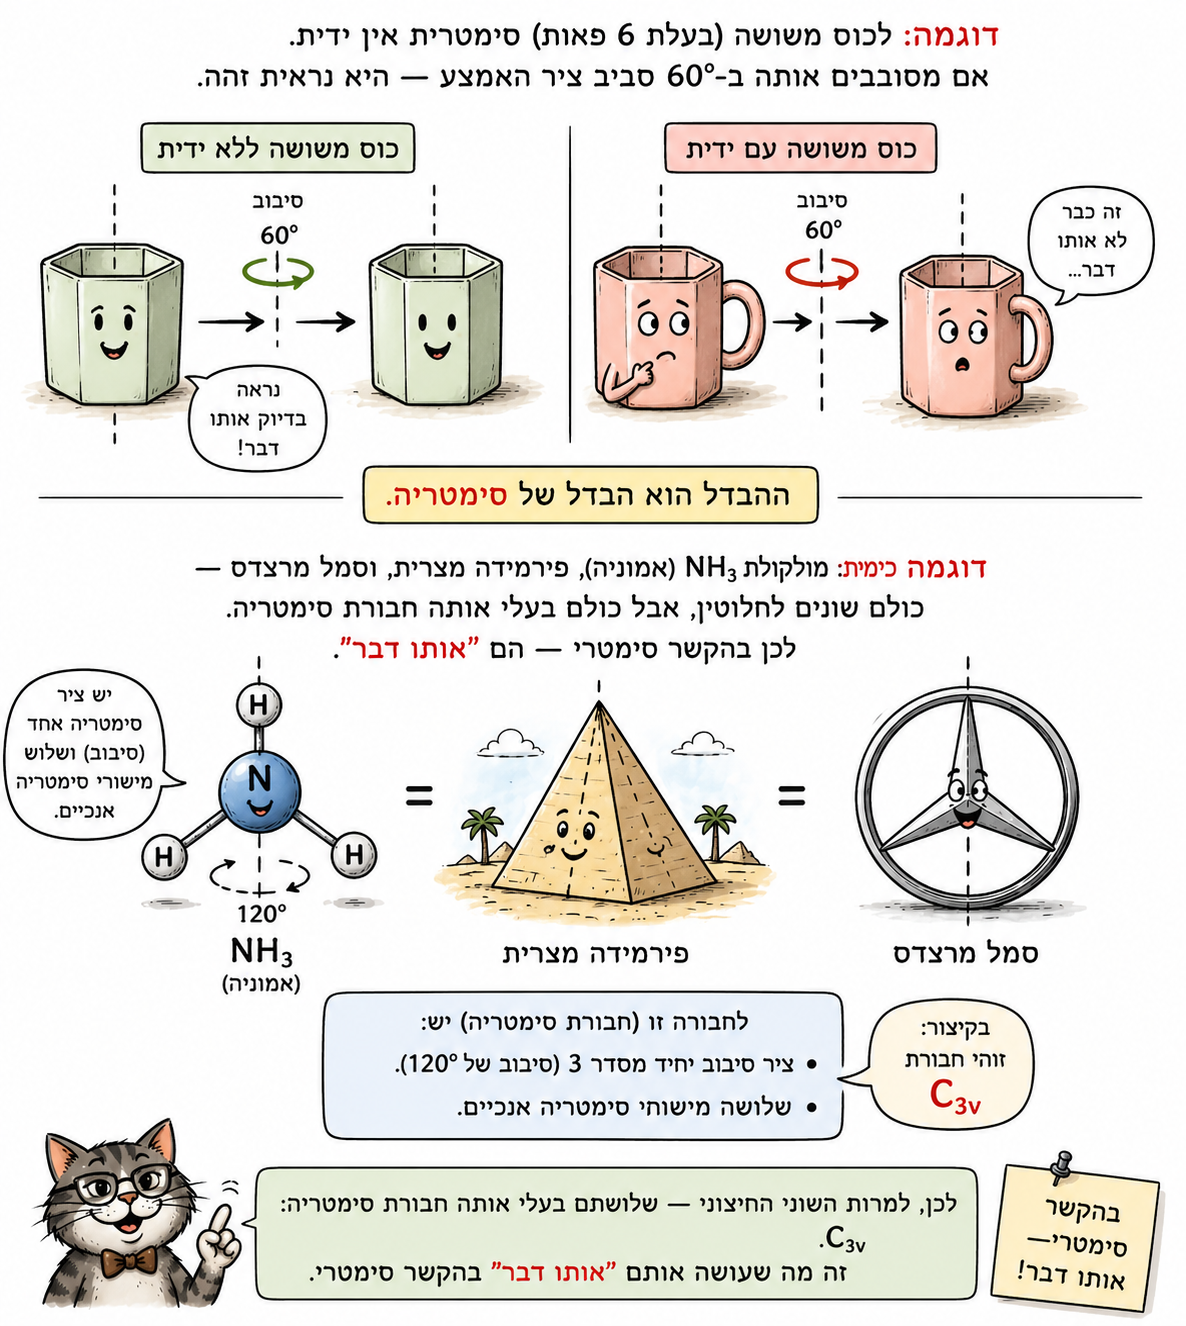
\includegraphics[keepaspectratio]{chapters/../images/image22.symmetry.png}}
\#\# 5.2 פעולות הסימטריה הבסיסיות

\subsection{\texorpdfstring{זהות --- \(E\)
(Identity)}{זהות --- E (Identity)}}\label{ux5d6ux5d4ux5d5ux5ea-e-identity}

``לא לעשות כלום'' --- העצם נשאר במקומו. זה נשמע טריוויאלי, אבל הכרחי
מבחינה מתמטית כדי שקבוצת הפעולות תהיה חבורה (ראו §5.4).

כל עצם בעולם בעל פעולת הזהות. \(E\) מסמלת \emph{Einheit} (אחדות
בגרמנית).

\subsection{\texorpdfstring{סיבוב --- \(C_n\)
(Rotation)}{סיבוב --- C\_n (Rotation)}}\label{ux5e1ux5d9ux5d1ux5d5ux5d1-c_n-rotation}

אם עצם יכול להסתובב בזווית \(\frac{360°}{n}\) סביב ציר כלשהו ולהישאר זהה
לעצמו --- יש לו \textbf{ציר סיבוב מסדר \(n\)}, מסומן \(C_n\).

\begin{itemize}
\tightlist
\item
  \(C_2\): סיבוב ב-\(180°\) (מולקולת \(\text{H}_2\text{O}\) סביב ציר
  הבי-סקטור)
\item
  \(C_3\): סיבוב ב-\(120°\) (אמוניה \(\text{NH}_3\) סביב ציר
  \(\text{N}\))
\item
  \(C_6\): סיבוב ב-\(60°\) (בנזן)
\item
  \(C_\infty\): כל זווית אפשרית --- מולקולה לינארית כמו \(\text{HCl}\)
\end{itemize}

אם אפשר לסובב פעמיים (ב-\(120°\) ואחר כך שוב ב-\(120°\)), זה \(C_3^2\).
שלוש פעמים חוזרים להתחלה: \(C_3^3 = E\).
\pandocbounded{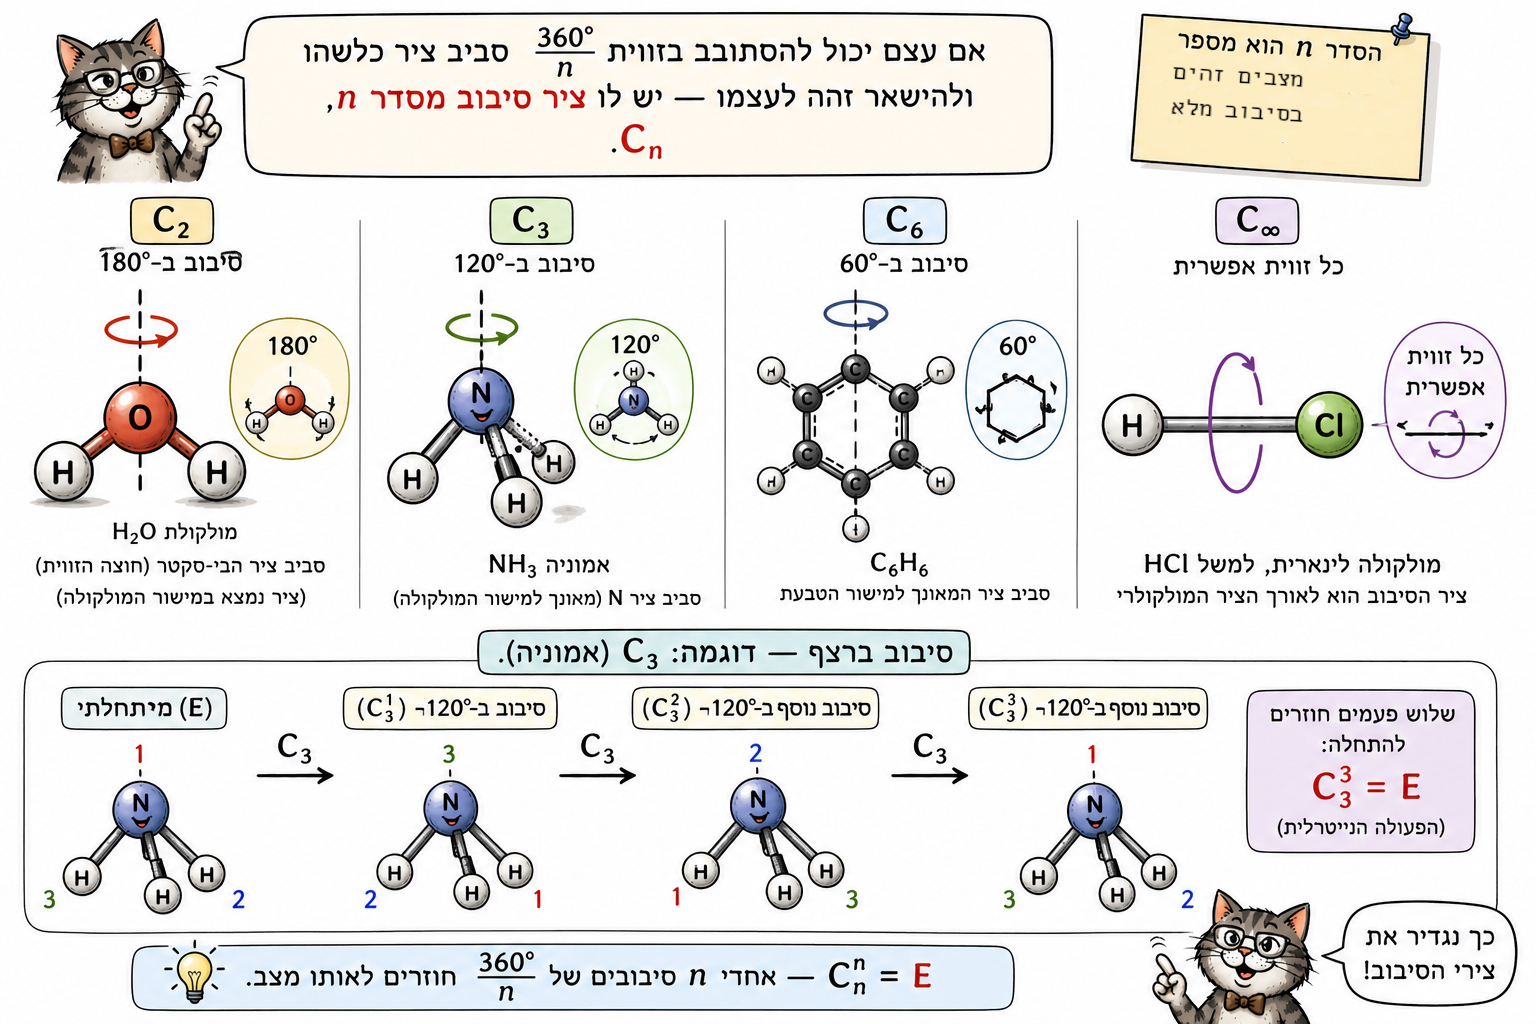
\includegraphics[keepaspectratio]{chapters/../images/image23.rotation.jpeg}}
\#\#\# שיקוף --- \(\sigma\) (Reflection)

אם עצם יכול להשתקף במישור ולהישאר זהה לעצמו --- יש לו \textbf{מישור
שיקוף} \(\sigma\).

\begin{itemize}
\tightlist
\item
  \(\sigma_h\) (horizontal): מישור \textbf{ניצב} לציר הראשי
\item
  \(\sigma_v\) (vertical): מישור \textbf{מכיל} את הציר הראשי
\item
  \(\sigma_d\) (dihedral): מישור אלכסוני, בין צירי \(C_2\) משניים
\end{itemize}

\pandocbounded{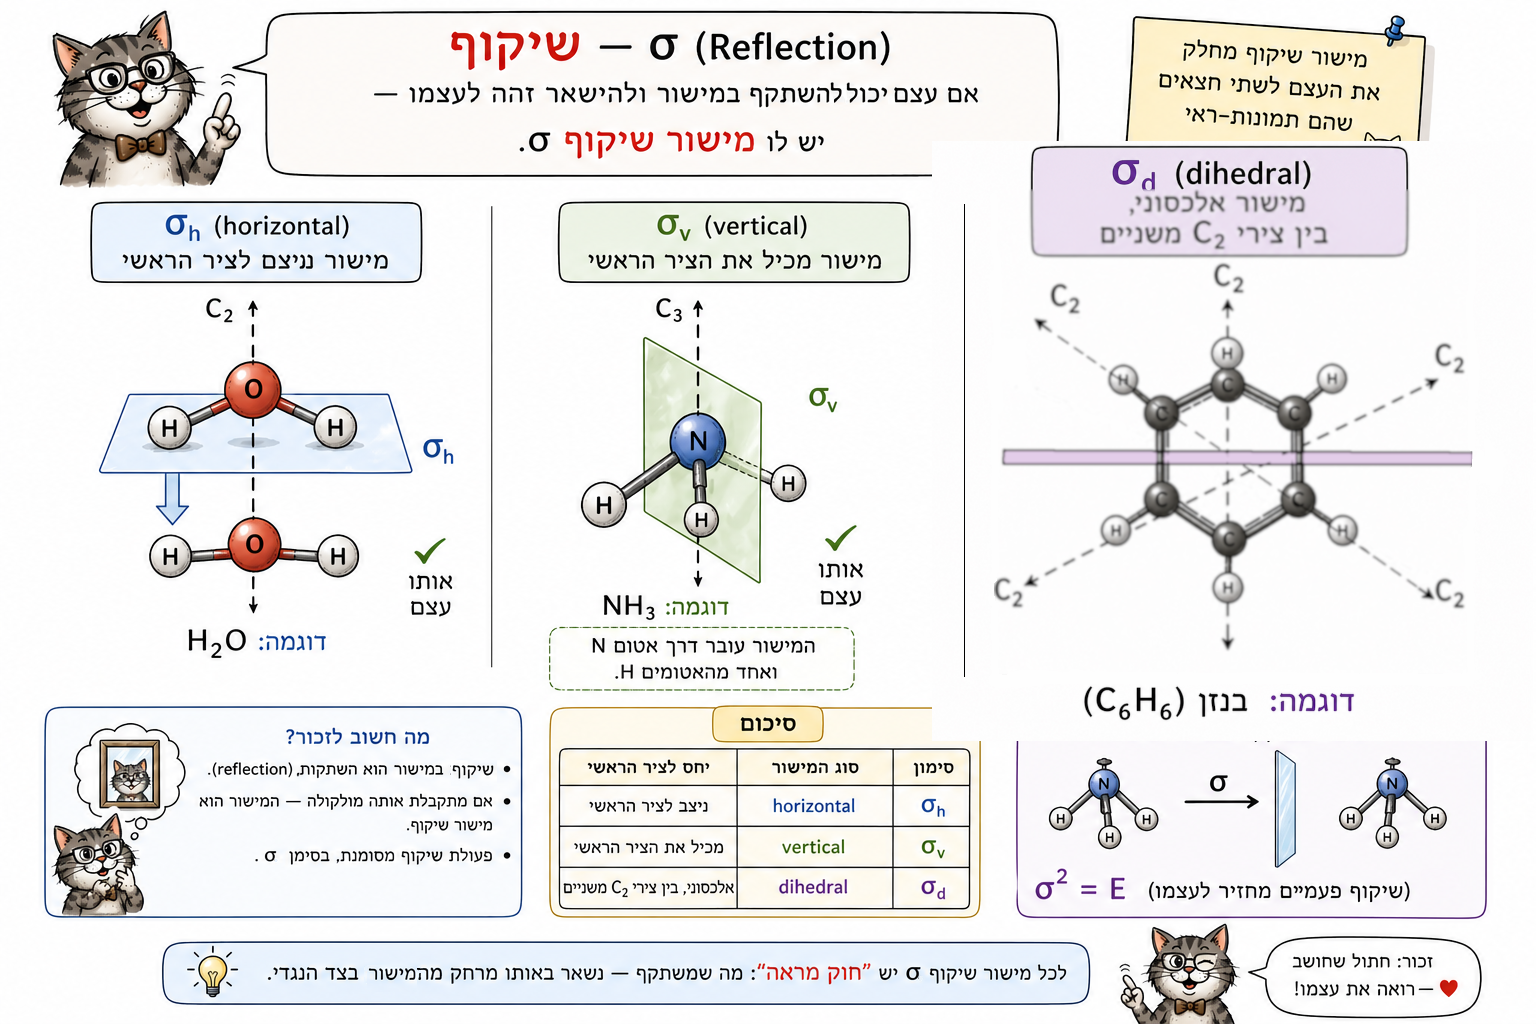
\includegraphics[keepaspectratio]{chapters/../images/image24.reflection.png}}
\#\#\# היפוך --- \(i\) (Inversion)\#\#\#

אם לכל נקודה \((x,y,z)\) במולקולה יש נקודה זהה ב-\((-x,-y,-z)\) --- יש
למולקולה \textbf{מרכז היפוך}.

\textbf{דוגמה:} \(\text{SF}_6\) (אוקטהדרי) --- כן. \(\text{NH}_3\)
(פירמידי) --- לא.
\pandocbounded{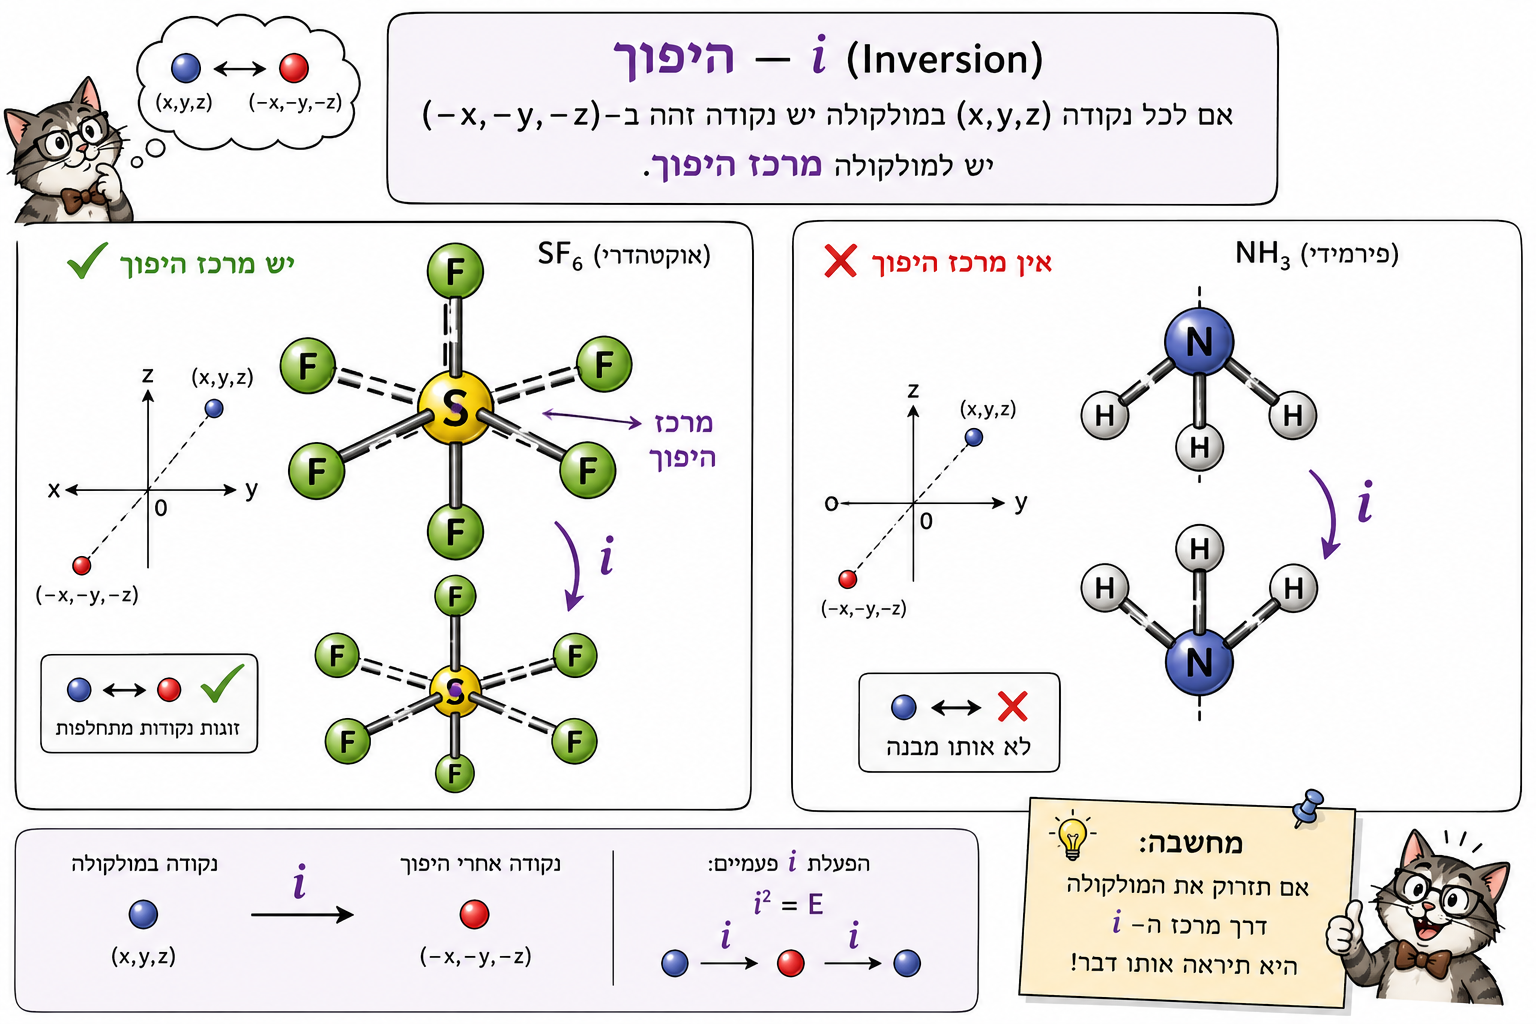
\includegraphics[keepaspectratio]{chapters/../images/image25.inversion.png}}
\#\#\# סיבוב מדומה --- \(S_n\) (Improper rotation)

פעולה מורכבת: \textbf{סיבוב ב-\(\frac{360°}{n}\)} ואחריו
\textbf{השתקפות} במישור הניצב לציר. אינטואיטיבית קשה לדמיין, אבל מתמטית
הכרחי.

\(S_1 = \sigma\) (מישור בלבד); \(S_2 = i\) (מרכז היפוך). כלומר, השתקפות
והיפוך הם מקרים פרטיים של \(S_n\).
\pandocbounded{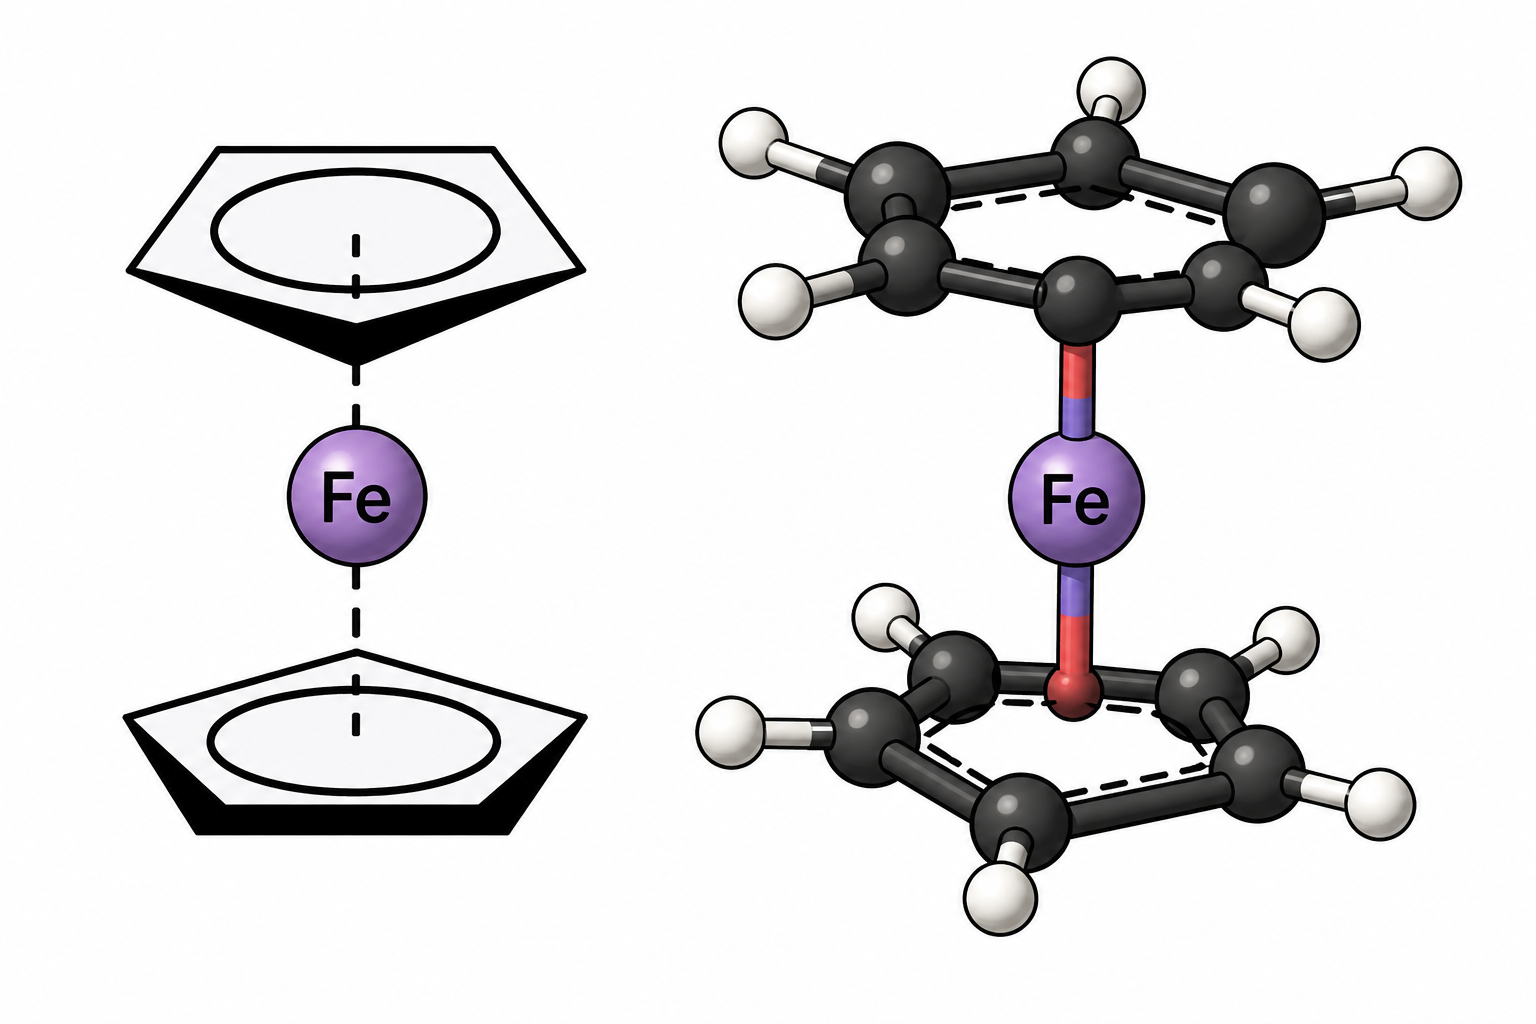
\includegraphics[keepaspectratio]{chapters/../images/image26.improperRotation.png}}
\#\# 5.3 חבורות נקודתיות --- אוסף פעולות הסימטריה של מולקולה

\subsection{מהי חבורת
נקודתית?}\label{ux5deux5d4ux5d9-ux5d7ux5d1ux5d5ux5e8ux5ea-ux5e0ux5e7ux5d5ux5d3ux5eaux5d9ux5ea}

\textbf{חבורת נקודתית} (point group) היא אוסף כל פעולות הסימטריה של
מולקולה, שכולן משמרות נקודה מרכזית אחת קבועה (מרכז המולקולה). שם החבורה
מתאר את הסימטריה במלואה.

הגדרה פורמלית:** קבוצת הפעולות שעהורה מתקיימןת ארבעת התנאים הבאים:

\begin{enumerate}
\def\labelenumi{\arabic{enumi}.}
\tightlist
\item
  \textbf{סגירות:} הרכבת כל שתי פעולות שבחבורה נותנת פעולה שנמצאת גם היא
  בחבורה
\item
  \textbf{אסוציאטיביות:} \((AB)C = A(BC)\)
\item
  \textbf{זהות:} קיימת פעולה \(E\) שאינה משנה דבר
\item
  \textbf{קיום הפכים:} לכל פעולה יש פעולה הפוכה (שמחזירה למצב ההתחלתי)
\end{enumerate}

\textbf{דוגמה --- חבורה \(C_{3v}\) (אמוניה \(\text{NH}_3\)):}

פעולות: \(E\), \(C_3^+\), \(C_3^-\), \(\sigma_v\), \(\sigma_v’\),
\(\sigma_v’’\) --- שש בסה''כ.
\pandocbounded{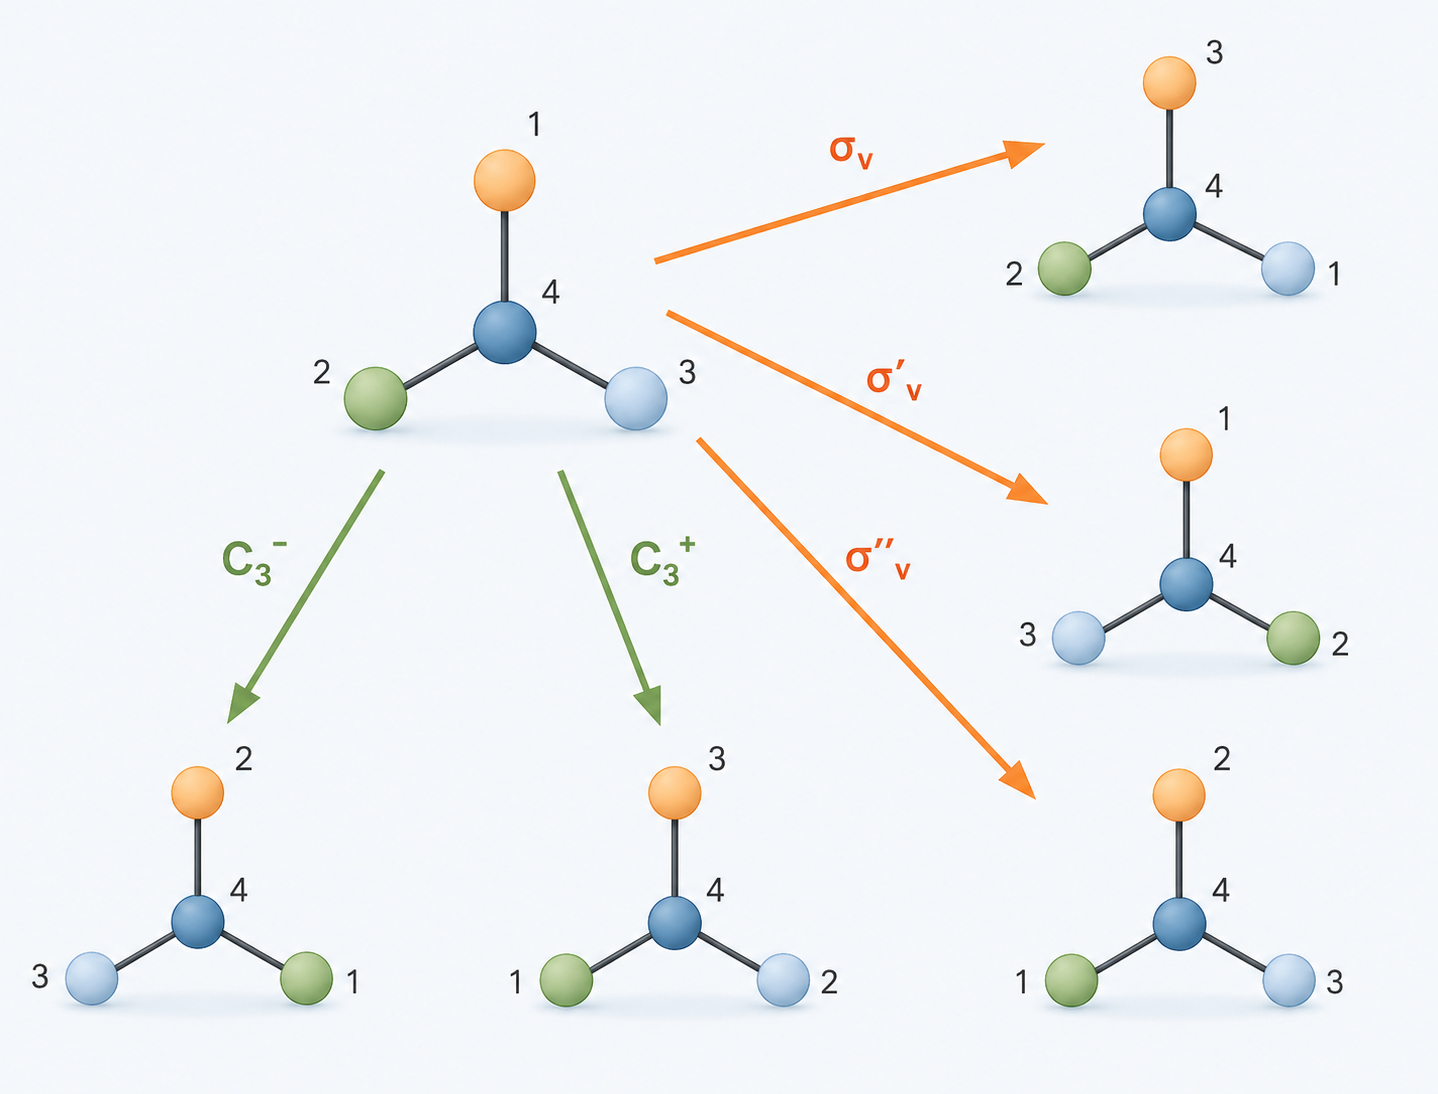
\includegraphics[keepaspectratio]{chapters/../images/image27.GroupC3v.jpeg}}
- \(C_3^+ \cdot C_3^+ = C_3^-\) (שני סיבובים של \(120°\) = סיבוב של
\(240°\)) - \(C_3^+ \cdot C_3^- = E\) (סיבוב ב-\(120°\) ואז ב-\(240°\) =
חזרה להתחלה) - \(C_3^+ \cdot \sigma_v = \sigma_v’\) (סיבוב ואחריו
השתקפות = השתקפות אחרת)

\subsection{32 חבורות
נקודתיות}\label{ux5d7ux5d1ux5d5ux5e8ux5d5ux5ea-ux5e0ux5e7ux5d5ux5d3ux5eaux5d9ux5d5ux5ea}

בתלת-ממד, קיימות בדיוק \textbf{32 חבורות נקודתיות} המסווגות לקטגוריות:

{\def\LTcaptype{none} % do not increment counter
\begin{longtable}[]{@{}lll@{}}
\toprule\noalign{}
קטגוריה & חבורות & דוגמת מולקולה \\
\midrule\noalign{}
\endhead
\bottomrule\noalign{}
\endlastfoot
לינארי & \(C_{\infty v}\), \(D_{\infty h}\) & HCl, CO₂ \\
מחזורי פשוט & \(C_1\), \(C_2\), \(C_3\), \(C_4\), \(C_6\) & --- \\
עם מישורים אנכיים & \(C_{2v}\), \(C_{3v}\), \(C_{4v}\) & H₂O, NH₃ \\
עם מישורים אופקיים & \(C_{2h}\), \(C_{3h}\) & --- \\
דיהדרלי & \(D_{2h}\), \(D_{3h}\), \(D_{6h}\) & C₂H₄, BF₃, בנזן \\
קובי & \(T_d\), \(O_h\) & CH₄, SF₆ \\
\end{longtable}
}

הסיומות: \emph{v} = ציר אנכי (vertical); \emph{h} = ציר אופקי
(horizontal); \emph{d} = אלכסוני (dihedral).
\pandocbounded{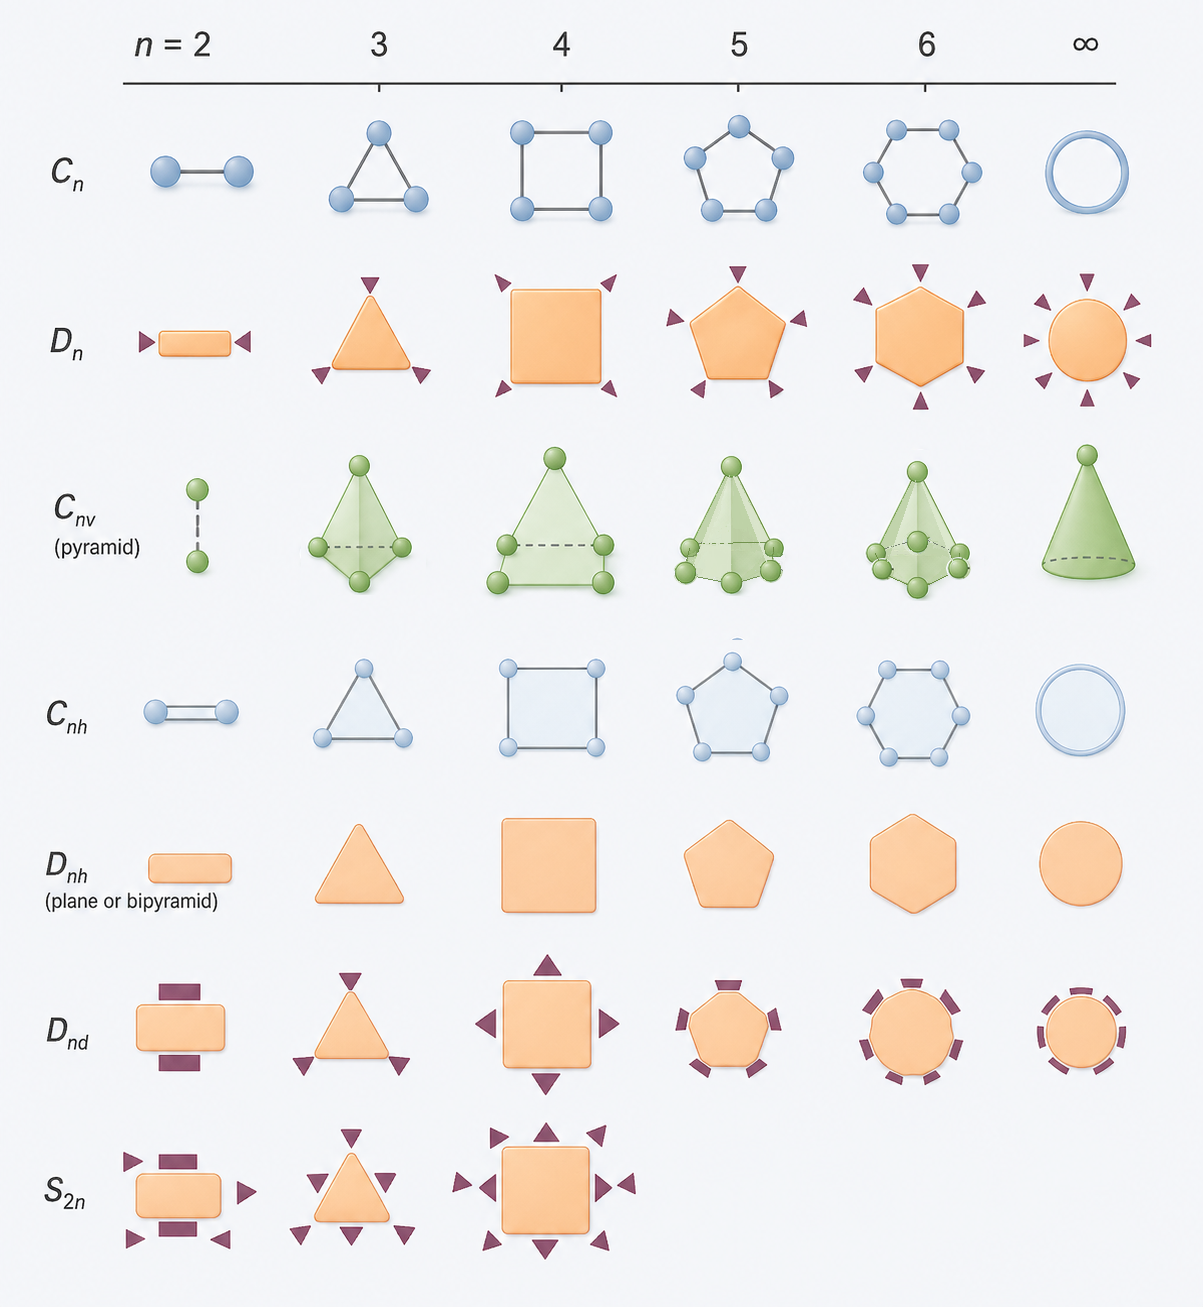
\includegraphics[keepaspectratio]{chapters/../images/image28.groups.png}}-----

\section{5.4 כיצד מזהים את חבורת הנקודה של
מולקולה?}\label{ux5dbux5d9ux5e6ux5d3-ux5deux5d6ux5d4ux5d9ux5dd-ux5d0ux5ea-ux5d7ux5d1ux5d5ux5e8ux5ea-ux5d4ux5e0ux5e7ux5d5ux5d3ux5d4-ux5e9ux5dc-ux5deux5d5ux5dcux5e7ux5d5ux5dcux5d4}

\textbf{אלגוריתם הזרימה} --- שאלות בסדר:

\textbf{1.} האם המולקולה \textbf{לינארית}?

\begin{itemize}
\tightlist
\item
  כן, עם מרכז היפוך → \(D_{\infty h}\) (CO₂, H₂, N₂)
\item
  כן, ללא מרכז היפוך → \(C_{\infty v}\) (HCl, CO, HCN)
\end{itemize}

\textbf{2.} האם יש \textbf{יותר מציר \(C_n\) אחד עם \(n>2\)}?

\begin{itemize}
\tightlist
\item
  כן → חבורות קוביות (\(T_d\) למולקולות טטרהדרליות כמו CH₄; \(O_h\)
  לאוקטהדרליות כמו SF₆)
\end{itemize}

\textbf{3.} מצא את \textbf{ציר \(C_n\) הראשי} (בעל \(n\) הגבוה ביותר).
האם יש \(n\) צירי \(C_2\) ניצבים אליו?

\begin{itemize}
\tightlist
\item
  כן → חבורות \(D\). בדוק מישורים: \(\sigma_h\) → \(D_{nh}\);
  \(\sigma_d\) → \(D_{nd}\); ללא → \(D_n\)
\item
  לא → חבורות \(C\). בדוק מישורים: \(\sigma_h\) → \(C_{nh}\);
  \(\sigma_v\) → \(C_{nv}\); ללא → \(C_n\)
\end{itemize}

\textbf{דוגמאות:}

\begin{itemize}
\tightlist
\item
  \(\text{H}*2\text{O}\): לא לינארית; ציר \(C_2\) ראשי; אין \(C_2\)
  ניצבים; יש שני \(\sigma_v\) → \textbf{\(C*{2v}\)}
\item
  \(\text{NH}*3\): ציר \(C_3\) ראשי; אין \(C_2\) ניצבים; יש שלושה
  \(\sigma_v\) → \textbf{\(C*{3v}\)}
\item
  בנזן: ציר \(C_6\) ראשי; יש \(C_2\) ניצבים; יש \(\sigma_h\) →
  \textbf{\(D_{6h}\)}
\item
  \(\text{CH}_4\): יש ארבעה צירי \(C_3\) → \textbf{\(T_d\)}
  \pandocbounded{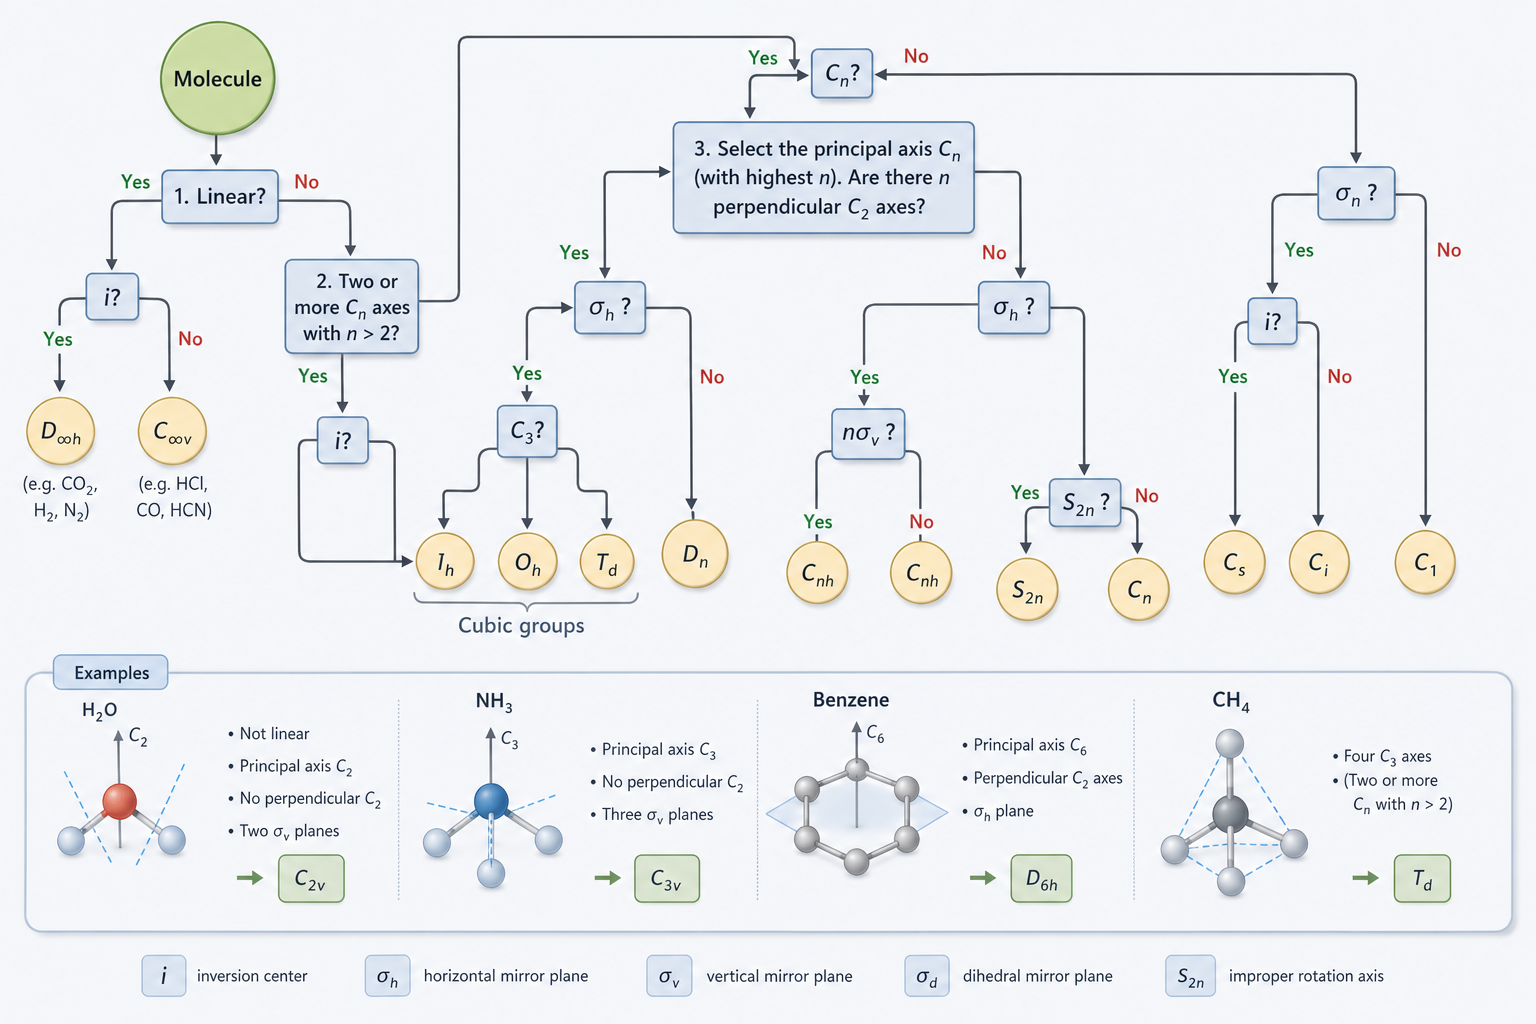
\includegraphics[keepaspectratio]{chapters/../images/image29.Groupdetermination.png}}
  \#\# 5.5 ייצוג של פעולות סימטריה במטריצות
\end{itemize}

\subsection{הרעיון}\label{ux5d4ux5e8ux5e2ux5d9ux5d5ux5df-1}

כדי \textbf{לחשב} עם סימטריה ולא רק לצייר תרשימים, נדרשת שפה מתמטית.
הכלי: \textbf{מטריצות}. כל פעולת סימטריה מיוצגת על ידי מטריצה, ופעולות
רצופות מחושבות על ידי כפל מטריצות.

\textbf{כיצד?} מייצגים את המולקולה כווקטור שורה של פרטי האטומים שלה, לפי
סדר מוסכם. לדוגמה, מולקולת \(C_{3v}\) עם ארבעה אטומים (N בציר, ושלושה
H):
\pandocbounded{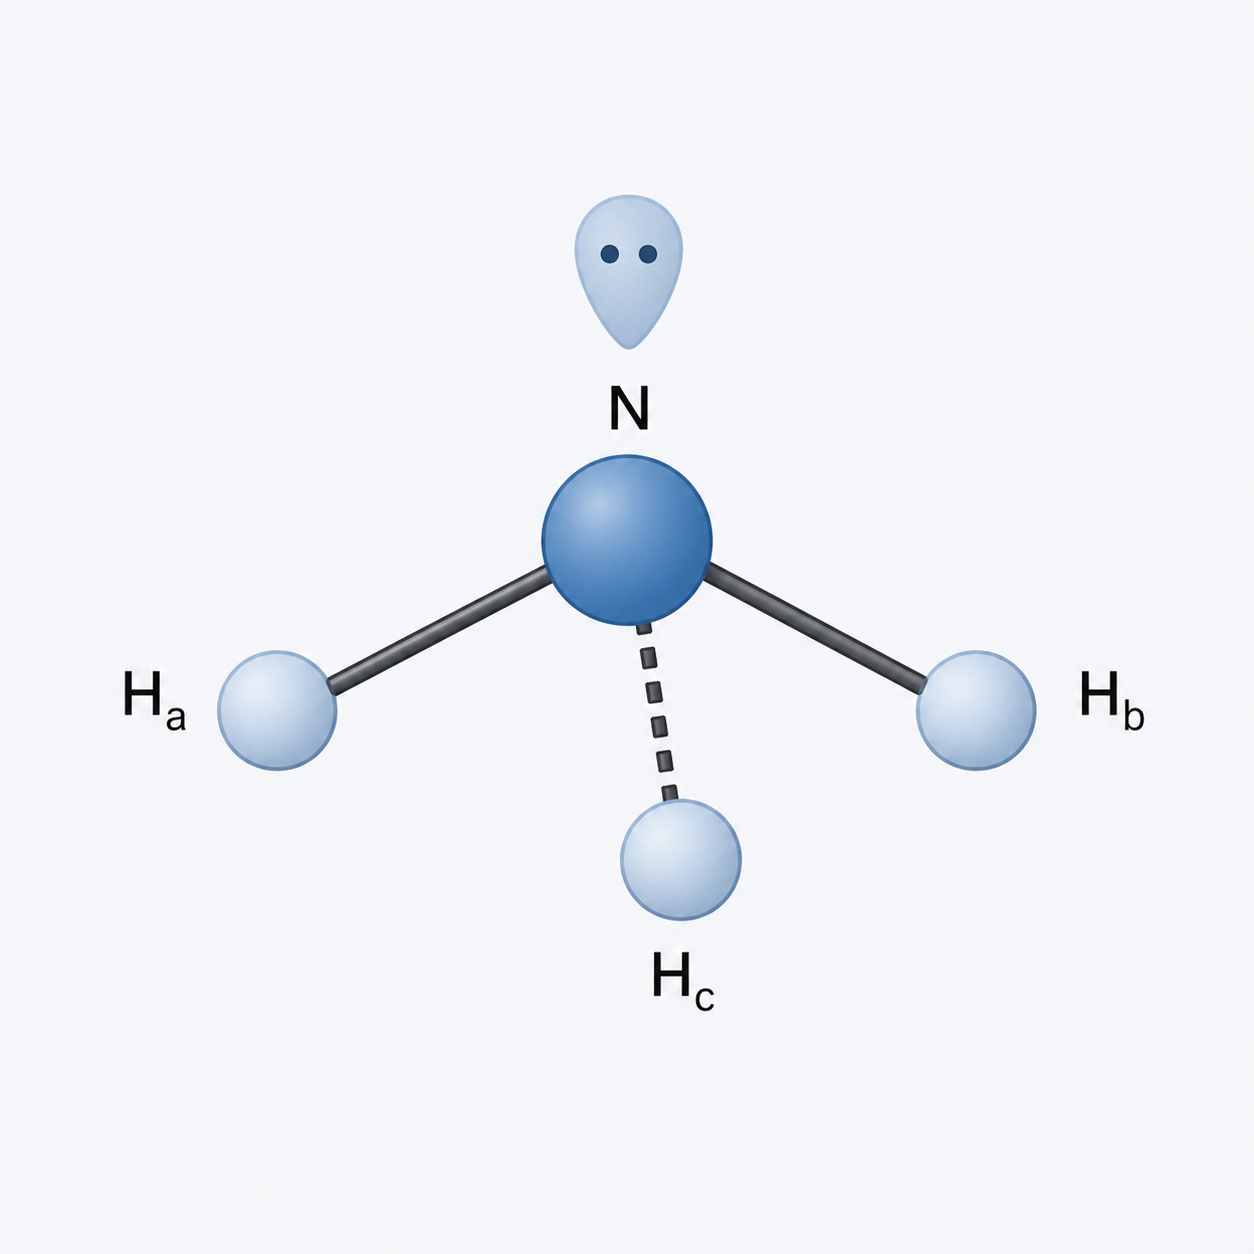
\includegraphics[keepaspectratio]{chapters/../images/image30.NH3.png}}

\[ \quad (N, H_a, H_b, H_c) = (4, 1, 2, 3)\]

פעולת \(\sigma_v\) (מישור שמשמר \(N\) ו-\(H_a\), ומחליף \(H_b\)
ו-\(H_c\)):

\[ \quad (4, 1, 3, 2)\]

הפעולה מתוארת על ידי מטריצה:

\[\sigma_v: \quad \begin{pmatrix} 1 & 0 & 0 & 0 \\ 0 & 1 & 0 & 0 \\ 0 & 0 & 0 & 1 \\ 0 & 0 & 1 & 0 \end{pmatrix}\]

\textbf{כלל מפתח:} אם אטום \textbf{לא זז} בפעולה --- יש \(1\) על
\textbf{האלכסון הראשי} (diagonal) של המטריצה. אם זז --- ה-\(1\) מחוץ
לאלכסון.

\subsection{האופי של
מטריצה}\label{ux5d4ux5d0ux5d5ux5e4ux5d9-ux5e9ux5dc-ux5deux5d8ux5e8ux5d9ux5e6ux5d4}

\pandocbounded{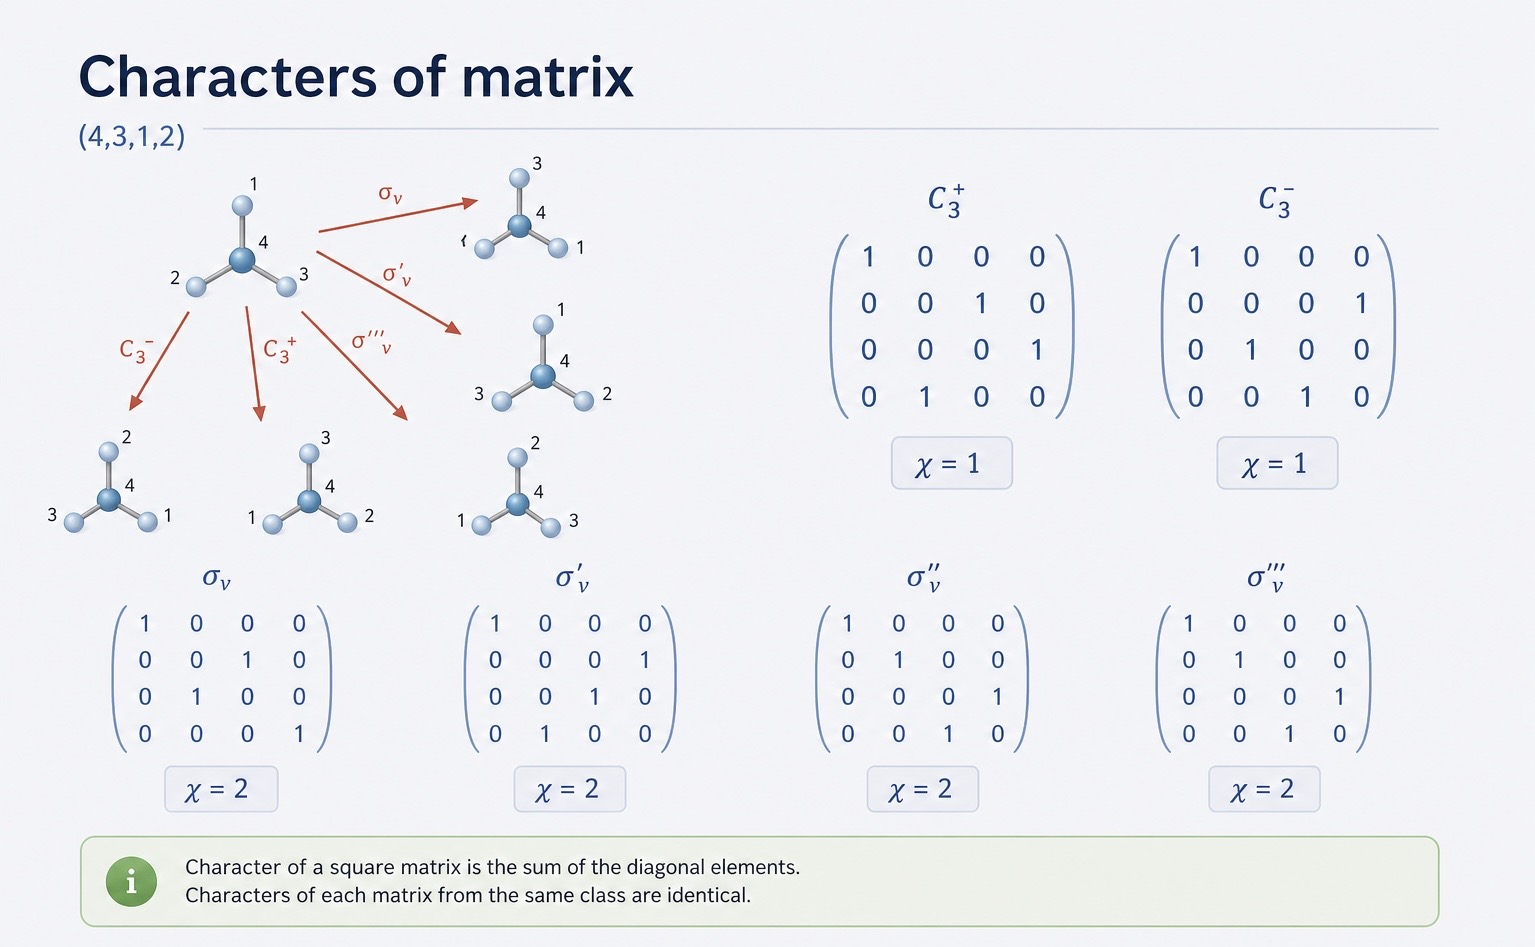
\includegraphics[keepaspectratio]{chapters/../images/image32.characters.jpeg}}\textbf{האופי
(character) \(\chi\) של מטריצה הוא }סכום האיברים על האלכסון הראשי**
(הנקרא גם טרייס, trace ביישומי מטריצות אחרים):

\[\chi = \sum_i M_{ii}\]

האופי שווה פשוט ל\textbf{מספר האטומים שלא זזו} בפעולה (עבור מטריצות
תמורה פשוטות).

לחבורה \(C_{3v}\) עם ארבעה אטומים:

{\def\LTcaptype{none} % do not increment counter
\begin{longtable}[]{@{}lll@{}}
\toprule\noalign{}
פעולה & אטומים שלא זזו & \(\chi\) \\
\midrule\noalign{}
\endhead
\bottomrule\noalign{}
\endlastfoot
\(E\) & כולם (4) & 4 \\
\(C_3^+\), \(C_3^-\) & רק N (1) & 1 \\
\(\sigma_v\), \(\sigma_v’\), \(\sigma_v’’\) & N + אחד מה-H (2) & 2 \\
\end{longtable}
}

\textbf{תכונה חשובה:} אופי של פעולות \textbf{מאותה מחלקה} (class) תמיד
זהים. לכן מספיק לשמור מספר אחד לכל מחלקה --- לא מטריצה שלמה. זה מקל על
החישוב.

\textbf{הצגות מטריצה} אם טרנספורמציות בחבורה נקודתית מיוצגות במטריצות,
ניתן לכנות אותן הצגות מטריצות. הצגת מטריצה היא מטריצה מרובעת המתארת
טרנספורמציה כלשהי המתבצעת בחבורה נקודתית. אם ניתן לצמצם את הצגה המטריצה
למטריצות קטנות יותר, הצגה זו נקראת פריקה. במקרה שבו לא ניתן לצמצם את
הצגת המטריצה עוד יותר, היא נקראת הצגה בלתי פריקה.
\pandocbounded{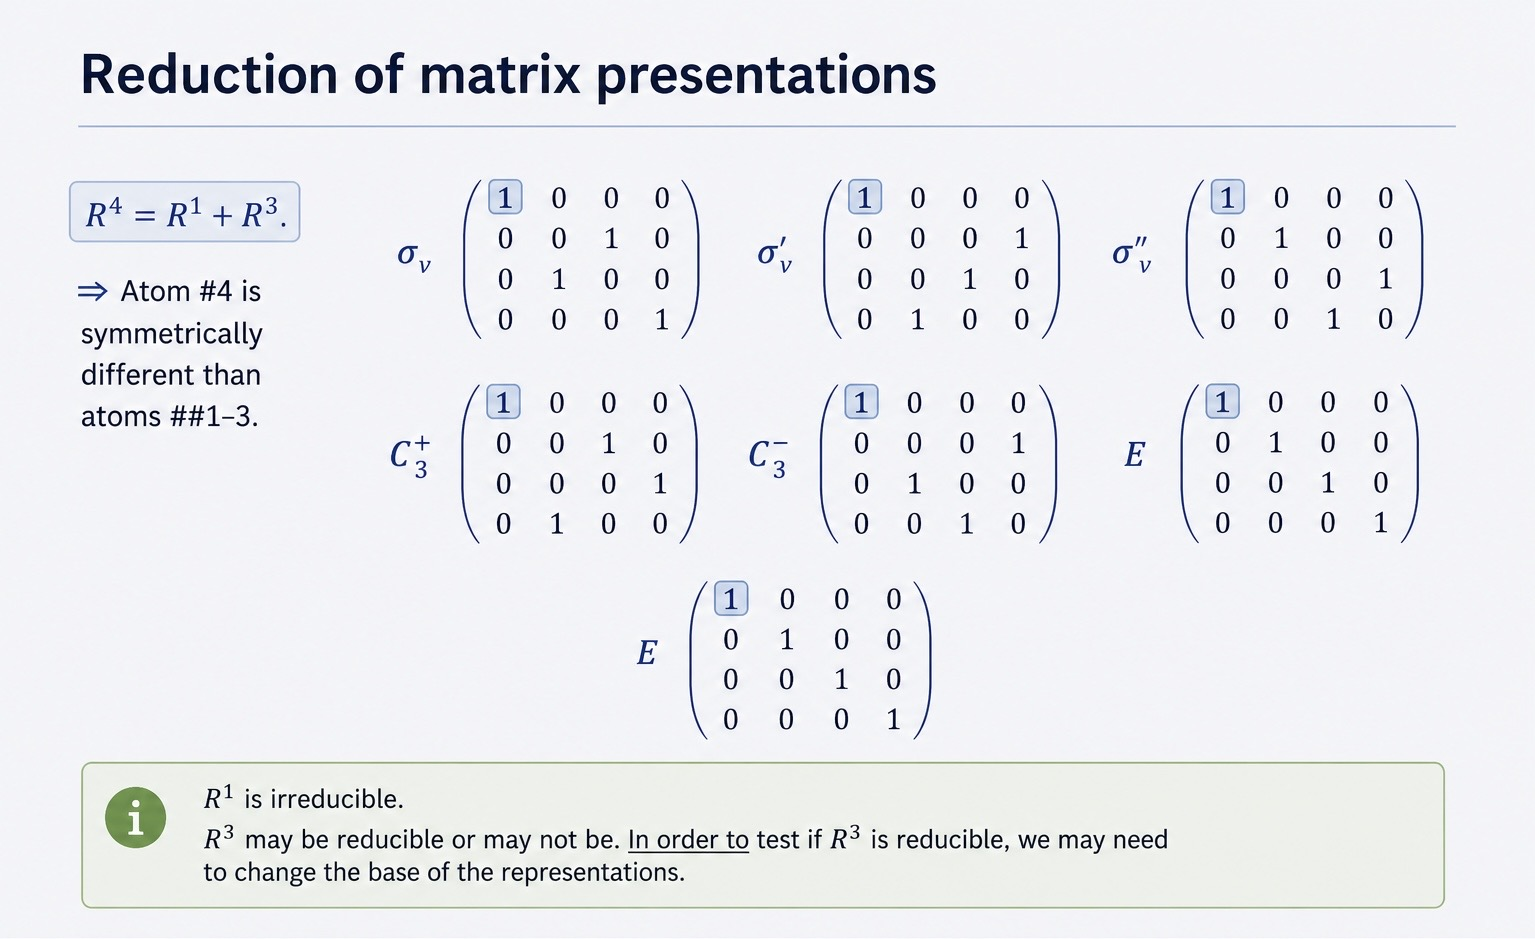
\includegraphics[keepaspectratio]{chapters/../images/image33.presentations.jpeg}}
\#\# 5.6 טבלאות אופי --- לב השיטה

\subsection{מהי טבלת
האופי?}\label{ux5deux5d4ux5d9-ux5d8ux5d1ux5dcux5ea-ux5d4ux5d0ux5d5ux5e4ux5d9}

לכל חבורת נקודתית מחושבת מראש \textbf{טבלת האופי} (character table).
הטבלאות נמצאות בכל ספר כימיה קוונטית ובמאגרים מקוונים. \textbf{לא צריך
לבנות אותן} --- רק לדעת לקרוא אותן.

\subsection{\texorpdfstring{מבנה הטבלה --- דוגמה \(C_{2v}\)
(מים)}{מבנה הטבלה --- דוגמה C\_\{2v\} (מים)}}\label{ux5deux5d1ux5e0ux5d4-ux5d4ux5d8ux5d1ux5dcux5d4-ux5d3ux5d5ux5d2ux5deux5d4-c_2v-ux5deux5d9ux5dd}

\[\begin{array}{c|cccc|cc}
C_{2v} & E & C_2 & \sigma_v(xz) & \sigma_v’(yz) & & \\
\hline
A_1 & 1 & 1 & 1 & 1 & z & x^2, y^2, z^2 \\
A_2 & 1 & 1 & -1 & -1 & R_z & xy \\
B_1 & 1 & -1 & 1 & -1 & x, R_y & xz \\
B_2 & 1 & -1 & -1 & 1 & y, R_x & yz \
\end{array}\]

\textbf{קריאת הטבלה:}

\begin{itemize}
\tightlist
\item
  \textbf{השורה העליונה:} שם החבורה, אחריו פעולות הסימטריה (מחלקה אחרי
  מחלקה)
\item
  \textbf{העמודה השמאלית:} שמות ה\textbf{הצגות הבלתי-פריקות}
  (irreducible representations) --- אלו בלוקי הבנייה הבסיסיים
\item
  \textbf{המספרים בטבלה:} האופי של כל הצגה תחת כל פעולה
\item
  \textbf{העמודה לפני האחרונה:} פונקציות לינאריות
  (\(x, y, z, R_x, R_y, R_z\)) --- מציינות אורביטלי p פעילים ב-IR
\item
  \textbf{העמודה האחרונה:} פונקציות ריבועיות (\(x^2, xy\)\ldots) ---
  מציינות אורביטלי d פעילים בראמן
\end{itemize}

\subsection{תוויות
מוליקן}\label{ux5eaux5d5ux5d5ux5d9ux5d5ux5ea-ux5deux5d5ux5dcux5d9ux5e7ux5df}

\pandocbounded{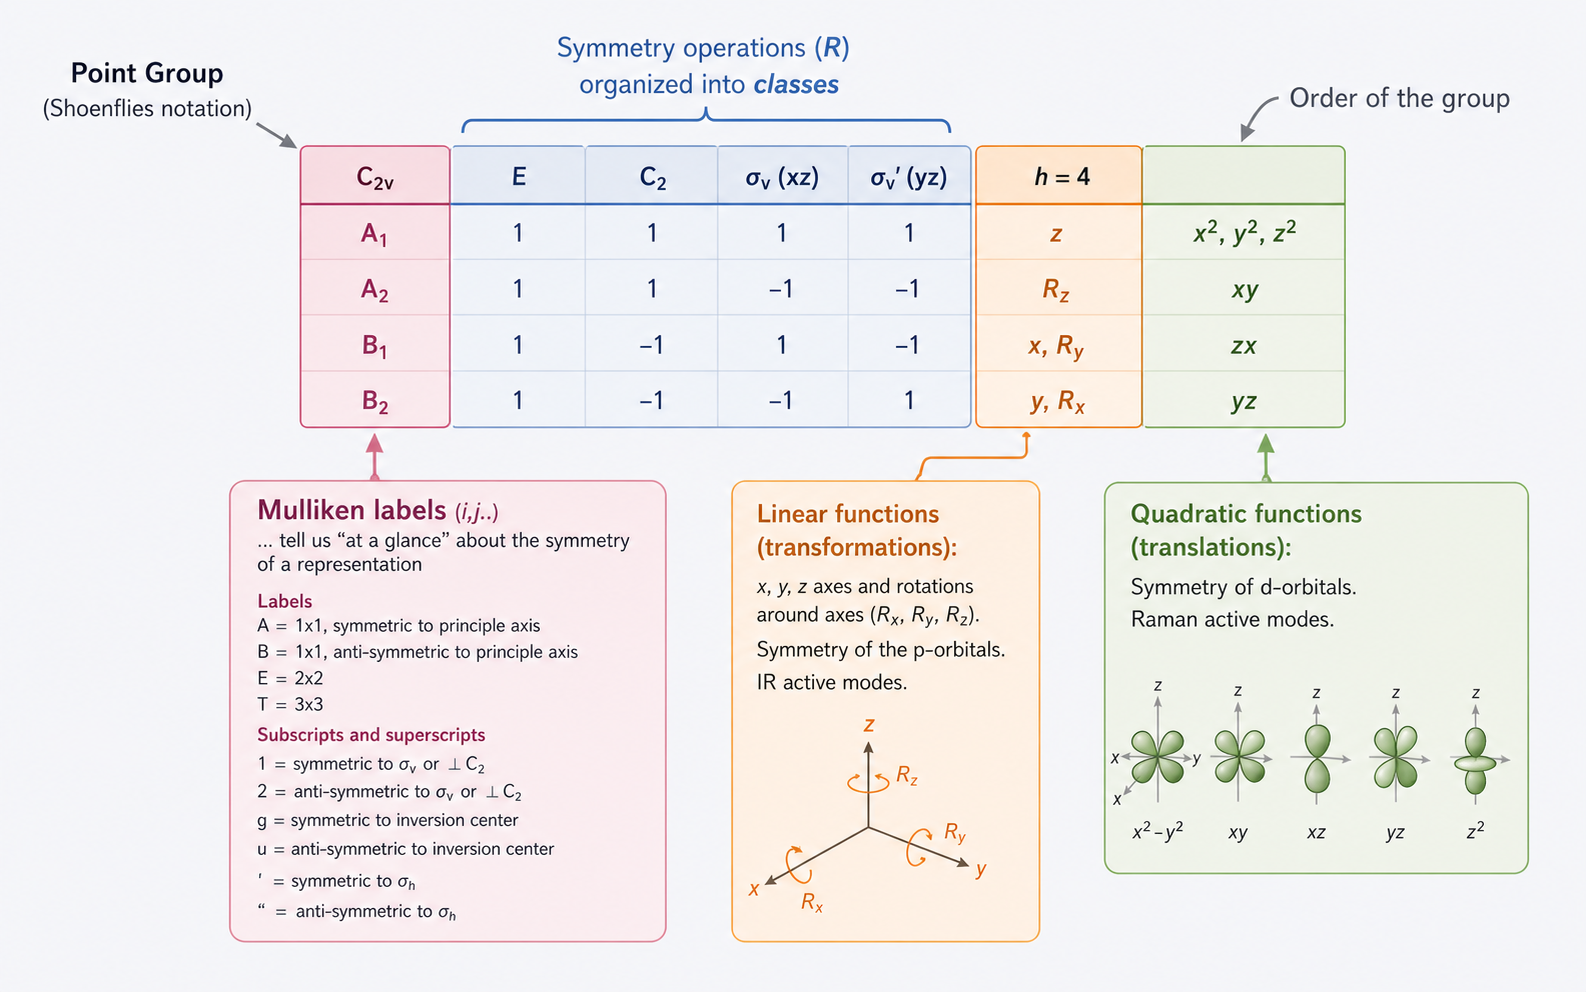
\includegraphics[keepaspectratio]{chapters/../images/image31.Mulliken.png}}
השמות \(A_1\), \(B_2\) וכד' הם \textbf{תוויות מוליקן} (Mulliken labels):

\begin{itemize}
\tightlist
\item
  \textbf{\(A\)}: סימטרי לגמרי ביחס לציר הראשי (האופי \(+1\) תחת
  \(C_n\))
\item
  \textbf{\(B\)}: אנטי-סימטרי ביחס לציר הראשי (האופי \(-1\) תחת \(C_n\))
\item
  \textbf{\(E\)}: הצגה \textbf{דו-ממדית} (מקבילה לשני אורביטלים מנוונים)
\item
  \textbf{\(T\)}: הצגה \textbf{תלת-ממדית}
\item
  אינדקס \textbf{\(1\)}: סימטרי ביחס ל-\(\sigma_v\) או לציר \(C_2\) משני
\item
  אינדקס \textbf{\(2\)}: אנטי-סימטרי ביחס לאלה
\item
  אינדקס \textbf{\(g\)} (gerade, ״זוגי״ בגרמנית): סימטרי ביחס למרכז
  היפוך
\item
  אינדקס \textbf{\(u\)} (ungerade, ״אי-זוגי״ בגרמנית): אנטי-סימטרי ביחס
  למרכז היפוך
\end{itemize}

\subsection{\texorpdfstring{מה אומר האופי \(+1\) ו-\(-1\)
?}{מה אומר האופי +1 ו-\/-1 ?}}\label{ux5deux5d4-ux5d0ux5d5ux5deux5e8-ux5d4ux5d0ux5d5ux5e4ux5d9-1-ux5d5--1}

\begin{itemize}
\tightlist
\item
  \(+1\): הפונקציה \textbf{לא משתנה} בפעולת הסימטריה הזו
\item
  \(-1\): הפונקציה \textbf{מחליפה סימן} (מוכפלת ב-\(-1\)) בהפעולה
\item
  \(0\): הפונקציה ``מתערבבת'' עם פונקציות אחרות (מתרחש בהצגות \(E\)
  ו-\(T\)) \#\# 5.7 (SALCs) קומבינציות לינאריות מותאמות-סימטריה
\end{itemize}

\subsection{הרעיון
המרכזי}\label{ux5d4ux5e8ux5e2ux5d9ux5d5ux5df-ux5d4ux5deux5e8ux5dbux5d6ux5d9}

כדי לבנות \textbf{אורביטלים מולקולריים} (MOs), אנחנו מחברים אורביטלים
אטומיים. אבל לא כל חיבור ``עובד'' --- רק אורביטלים מאותה סימטריה
מתחברים.

אורביטלי \textbf{SALCs} (Symmetry-Adapted Linear Combinations) הן
קומבינציות לינאריות של אורביטלים אטומיים שבנויות לפי סימטריית המולקולה.
במקום לבדוק כל צירוף --- בונים קומבינציות שמותאמות לסימטריה, ואז רק
קומבינציות מאותה הצגה מתחברות.

\textbf{יתרון:} במקום בעיה גדולה אחת (לדוגמה, מטריצה \(10 \times 10\)),
מקבלים כמה בעיות קטנות נפרדות --- אחת לכל הצגה. פשוט הרבה יותר.

\textbf{\emph{אלגוריתם העבודה עם SALCs}} \textbf{\emph{שלב ראשון:}}
בניית ה-SALCs --- עובדים רק עם הליגנדים (האטומים או קבוצות האטומים
הקשורים לאטום המרכזי). ה-SALCs הם קומבינציות של אורביטלים אטומיים של
הליגנדים בלבד. האטום המרכזי אינו משתתף בשלב זה כלל. למשל, במקרה של NH₃
אנחנו מתחילים משלושת אורביטלי ה-1s של שלושת המימנים ובונים מהם
קומבינציות המותאמות לסימטריה של המולקולה. התוצאה: שלושה SALCs --- אחד
מסוג A₁ ושניים מסוג E. שימו לב: מספר האורביטלים לא משתנה: נלקחו שלושה AO
של המימנים והתקבלו שלושה SALCs. \textbf{\emph{שלב שני:}} התאמה לאורביטלי
האטום המרכזי. רק עכשיו מסתכלים על אורביטלי החנקן ושואלים: אילו מהם
תואמים בסימטריה לכל אחד מה-SALCs? אורביטל של האטום המרכזי יכול ליצור
אורביטל מולקולרי קשור רק עם SALC בעל אותה סימטריה. אם אין SALC מתאים ---
האורביטל נשאר לא-קשור.

\textbf{\emph{הערה חשובה 1}}: בשיטה ה-SALCs אנחנו מתמקדים בליגנדים ולא
באטום המרכזי.הדבר עשוי להרגיש הפוך מהרגיל --- הרי בדרך כלל האטום המרכזי
הוא ``הכוכב'' של המולקולה. הבעיה האמיתית אומנם, היא שיש לנו כמה
אורביטלים של הליגנדים , ואנחנו לא יודעים כיצד להשוות כל אחד מהם בנפרד
לאורביטלי האטום המרכזי. ב-SALCs אנחנו ``מסרקים'' את אורביטלי הליגנדים
ומארגנים אותם לפי סימטריה. אחרי זה ההשוואה לאטום המרכזי הופכת לפשוטה ---
אם הסימטריות תואמות, יש אינטראקציה; אם לא --- אין, נקודה. \emph{כלומר,
ה-SALCs הם כלי עזר שנבנה למען האטום המרכזי, לא במקומו.}

\textbf{\emph{הערה חשובה 2:}} האם ה-SALCs הם אורביטלים ``אמיתיים'' או
המצאה מתמטית? ה-SALCs אמיתיים בדיוק באותו מובן שבו אורביטלים היברידיים
הם אמיתיים. כשאנחנו בונים אורביטל sp³ של פחמן, אנחנו גם לוקחים אורביטלים
אטומיים ובונים מהם קומבינציה לינארית --- אורביטל כזה לא קיים באטום פחמן
מבודד, אבל הוא מתאר נכון את המציאות במולקולה. בדיוק כך ה-SALCs: הם
קומבינציות של אורביטלי הליגנדים שמשקפות את הסימטריה האמיתית של המולקולה.
יתרה מזאת --- ה-SALCs מתגלים ניסיונית: בספקטרוסקופיית פוטואלקטרונים
(PES) רואים פסים נפרדים התואמים לסימטריות שונות, בדיוק כפי שהתיאוריה
מנבאת. \#\#\# אלגוריתם בארבעה שלבים

\textbf{שלב 1 --- בניית הצגה פריקה:}

עבור כל פעולת סימטריה, סופרים:

\begin{itemize}
\tightlist
\item
  \(+1\): האורביטל נשאר במקומו
\item
  \(0\): האורביטל עובר לאטום אחר
\item
  \(-1\): האורביטל נשאר אך מחליף סימן
\end{itemize}

התוצאה היא שורת אופי ---\textbf{הצגה פריקה} \(\Gamma\).

\textbf{שלב 2 --- פירוק להצגות בלתי-פריקות:}

באמצעות \textbf{נוסחת הצמצום}:

\[n_i = \frac{1}{h} \sum_R \chi(\Gamma) \cdot \chi_i(R)\]

כאשר \(h\) הוא סדר החבורה (מספר הפעולות הכולל), \(\chi(\Gamma)\) הוא
האופי של ההצגה שבנינו, ו-\(\chi_i(R)\) הוא האופי מטבלת האופי. \(n_i\)
הוא כמה פעמים ההצגה \(i\) מופיעה.

\textbf{שלב 3 --- אופרטור ההטלה:}

לכל הצגה בלתי-פריקה, מפעילים את כל פעולות הסימטריה על אורביטל אחד,
מכפילים באופי המתאים, ומסכמים.

\textbf{שלב 4 --- נירמול:}

\[N = \frac{1}{\sqrt{\sum_i c_i^2}}\]

כאשר \(c_i\) הם המקדמים שקיבלנו. כופלים את ה-SALC ב-\(N\) כדי שיהיה
מנורמל.

\subsection{\texorpdfstring{דוגמה מלאה: \(\text{NH}*3\) (חבורה
\(C_{3v}\))}{דוגמה מלאה: \textbackslash text\{NH\}*3 (חבורה C\_\{3v\})}}\label{ux5d3ux5d5ux5d2ux5deux5d4-ux5deux5dcux5d0ux5d4-textnh3-ux5d7ux5d1ux5d5ux5e8ux5d4-c_3v}

\textbf{הגדרה:} שלושה אורביטלי \(1s\) של אטומי המימן, מסומנים
\(\psi_a\), \(\psi_b\), \(\psi_c\).

\textbf{טבלת כאופי של \(C_{3v}\):}

{\def\LTcaptype{none} % do not increment counter
\begin{longtable}[]{@{}
  >{\raggedright\arraybackslash}p{(\linewidth - 10\tabcolsep) * \real{0.1481}}
  >{\raggedright\arraybackslash}p{(\linewidth - 10\tabcolsep) * \real{0.0556}}
  >{\raggedright\arraybackslash}p{(\linewidth - 10\tabcolsep) * \real{0.1111}}
  >{\raggedright\arraybackslash}p{(\linewidth - 10\tabcolsep) * \real{0.2037}}
  >{\raggedright\arraybackslash}p{(\linewidth - 10\tabcolsep) * \real{0.0926}}
  >{\raggedright\arraybackslash}p{(\linewidth - 10\tabcolsep) * \real{0.3889}}@{}}
\toprule\noalign{}
\begin{minipage}[b]{\linewidth}\raggedright
\(C_{3v}\)
\end{minipage} & \begin{minipage}[b]{\linewidth}\raggedright
\(E\)
\end{minipage} & \begin{minipage}[b]{\linewidth}\raggedright
\(2C_3\)
\end{minipage} & \begin{minipage}[b]{\linewidth}\raggedright
\(3\sigma_v\)
\end{minipage} & \begin{minipage}[b]{\linewidth}\raggedright
\end{minipage} & \begin{minipage}[b]{\linewidth}\raggedright
\end{minipage} \\
\midrule\noalign{}
\endhead
\bottomrule\noalign{}
\endlastfoot
\(A_1\) & 1 & 1 & 1 & \(z\) & \(x^2+y^2, z^2\) \\
\(A_2\) & 1 & 1 & \(-1\) & \(R_z\) & \\
\(E\) & 2 & \(-1\) & 0 & \(x,y\) & \(x^2-y^2, xy, xz, yz\) \\
\end{longtable}
}

\textbf{שלב 1:} תחת \(E\) --- שלושתם במקומם (\(\chi=3\)); תחת \(C_3\)
--- כולם זזים (\(\chi=0\)); תחת \(\sigma_v\) --- אחד נשאר (\(\chi=1\)):

\[\Gamma_s(H): \quad E=3,\quad 2C_3=0,\quad 3\sigma_v=1\]

\textbf{שלב 2 --- פירוק} (סדר החבורה \(h=6\)):

\[n(A_1) = \frac{1}{6}[1\cdot3\cdot1 + 2\cdot0\cdot1 + 3\cdot1\cdot1] = \frac{1}{6}[3+0+3] = 1\]

\[n(A_2) = \frac{1}{6}[1\cdot3\cdot1 + 2\cdot0\cdot1 + 3\cdot1\cdot(-1)] = \frac{1}{6}[3+0-3] = 0\]

\[n(E) = \frac{1}{6}[1\cdot3\cdot2 + 2\cdot0\cdot(-1) + 3\cdot1\cdot0] = \frac{1}{6}[6+0+0] = 1\]

\textbf{תוצאה:} \(\Gamma_s(H) = A_1 + E\)

\textbf{שלב 3--4 --- ה-SALCs:}

\[\text{SALC}(A_1) = \frac{1}{\sqrt{3}}\left(\psi_a + \psi_b + \psi_c\right)\]

\[\text{SALC}_1(E) = \frac{1}{\sqrt{6}}\left(2\psi_a - \psi_b - \psi_c\right)\]

\[\text{SALC}_2(E) = \frac{1}{\sqrt{2}}\left(\psi_b - \psi_c\right)\]
\pandocbounded{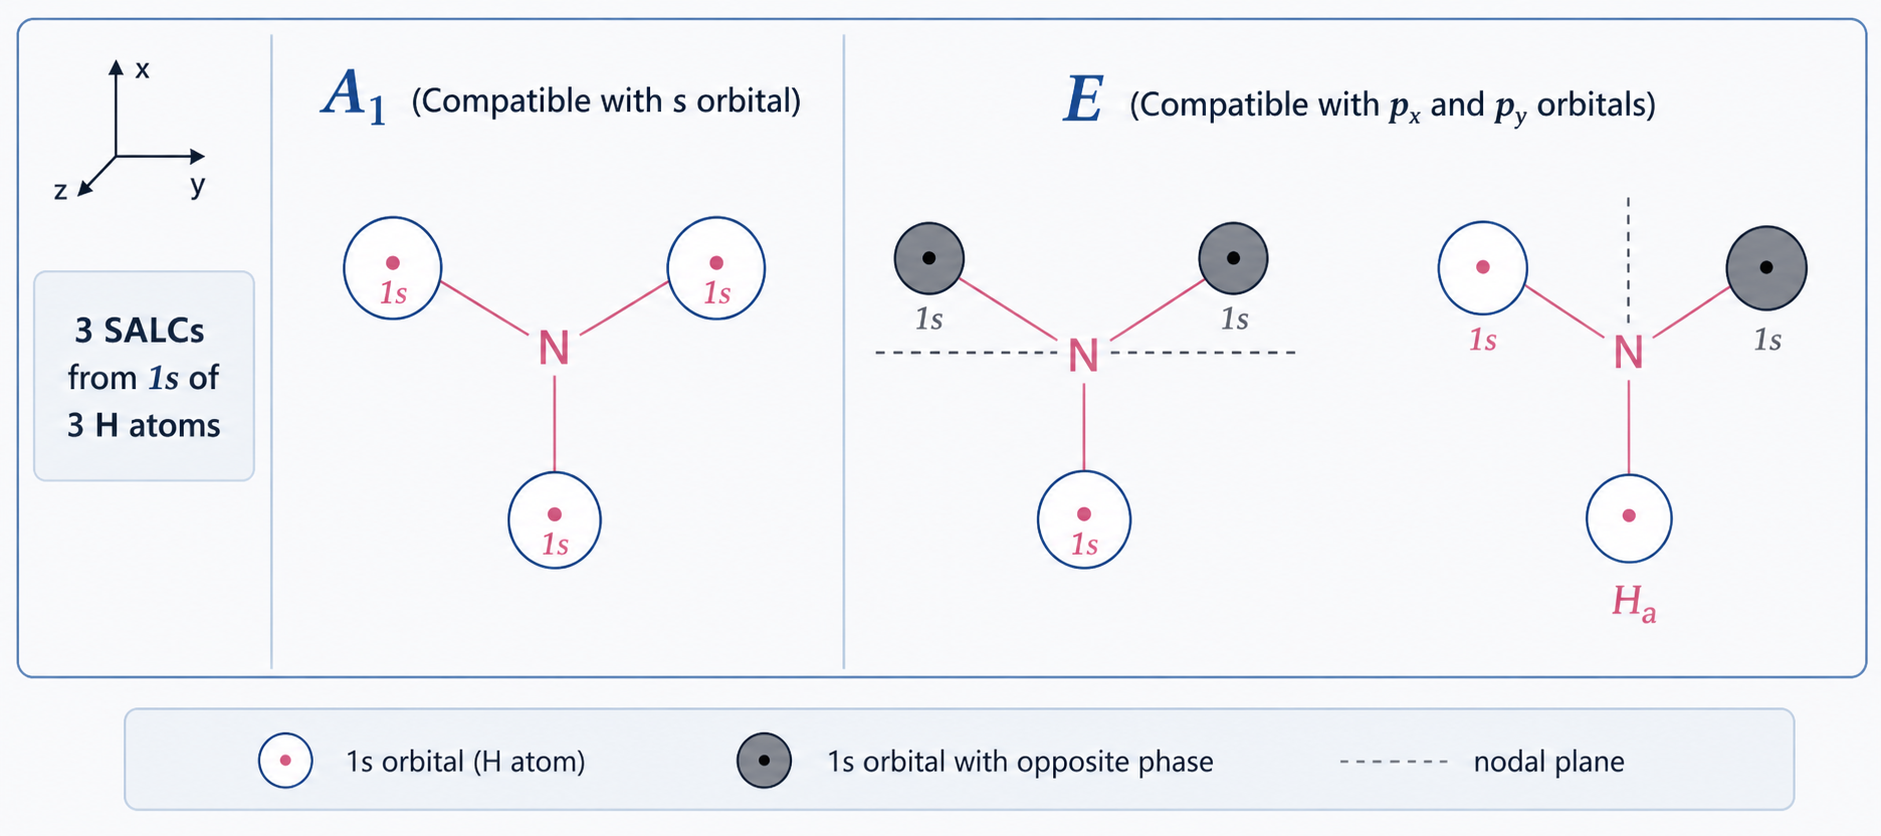
\includegraphics[keepaspectratio]{chapters/../images/image34.SALCs.png}}
\#\#\# מה עושים עם ה-SALCs?

עכשיו בודקים אורביטלי אטום החנקן ורואים מה יש להם אותה סימטריה:

\begin{itemize}
\tightlist
\item
  \(2s_N \to A_1\) (כדורי, סימטרי לגמרי)
\item
  \(2p_z \to A_1\) (ציר ה-\(z\) הוא ציר הסימטריה)
\item
  \(2p_x, 2p_y \to E\) (זוג מנוון)
\end{itemize}

\textbf{מסקנה:} לאורביטלי האטום של החנקן \(2s\) ו-\(2p_z\) יש אותה
סימטריה A₁, ולכן שניהם יכולים להשתתף ביצירת אורביטלים מולקולריים מסוג
A₁. בפועל, שני ה-MOs מסוג A₁ הם תערובות של \emph{2s}, \(2p_z\) ושל
ה-SALC-A₁ של מימני המימן --- אחד קשור ואחד לא-קשור (בעיקרו). האורביטלים
\(2p_x\) ו-\(2p_y\) של החנקן הם זוג מנוון מסוג E, ולכן הם מתחברים עם זוג
ה-SALCs מסוג E של המימן. כל אחד מהם מתחבר עם ה-SALC המתאים לו --- הם
אינם מתערבבים זה עם זה. לאורביטלי ה-SALC של המימן אין ייצוג מסוג A₂, וגם
בין אורביטלי החנקן אין אורביטל בעל סימטריה A₂ (וזה למרות שהצגה זאת
מופיעה בטבלת האופי). לכן A₂ אינו מופיע כלל בבניית ה-MOs של NH₃. סיכום:
עבור ההצגה \(A_1\): -אורביטל ה-SALC-A1 של המימנים מתחבר \textbf{רק} עם
\(2s_N\) ועם \(2p_z\) (שניהם \(A_1\)) עבור ההצגה \(E\): -אורביטל
ה-SALC-E (המכיל שני אורביטלים מנוונים) של המימנים מתחבר \textbf{רק} עם
\(2p_x\) ועם \(2p_y\) (שניהם \(E\)) עבור ההצגה \(A_2\): אין אורביטל עם
סימטריה זאת בין ה-SALCs וגם אים בין ה-AO של החנקן. על כן, הצגה זאצ אינה
מתאימה לאף קשר במולקולה.
\pandocbounded{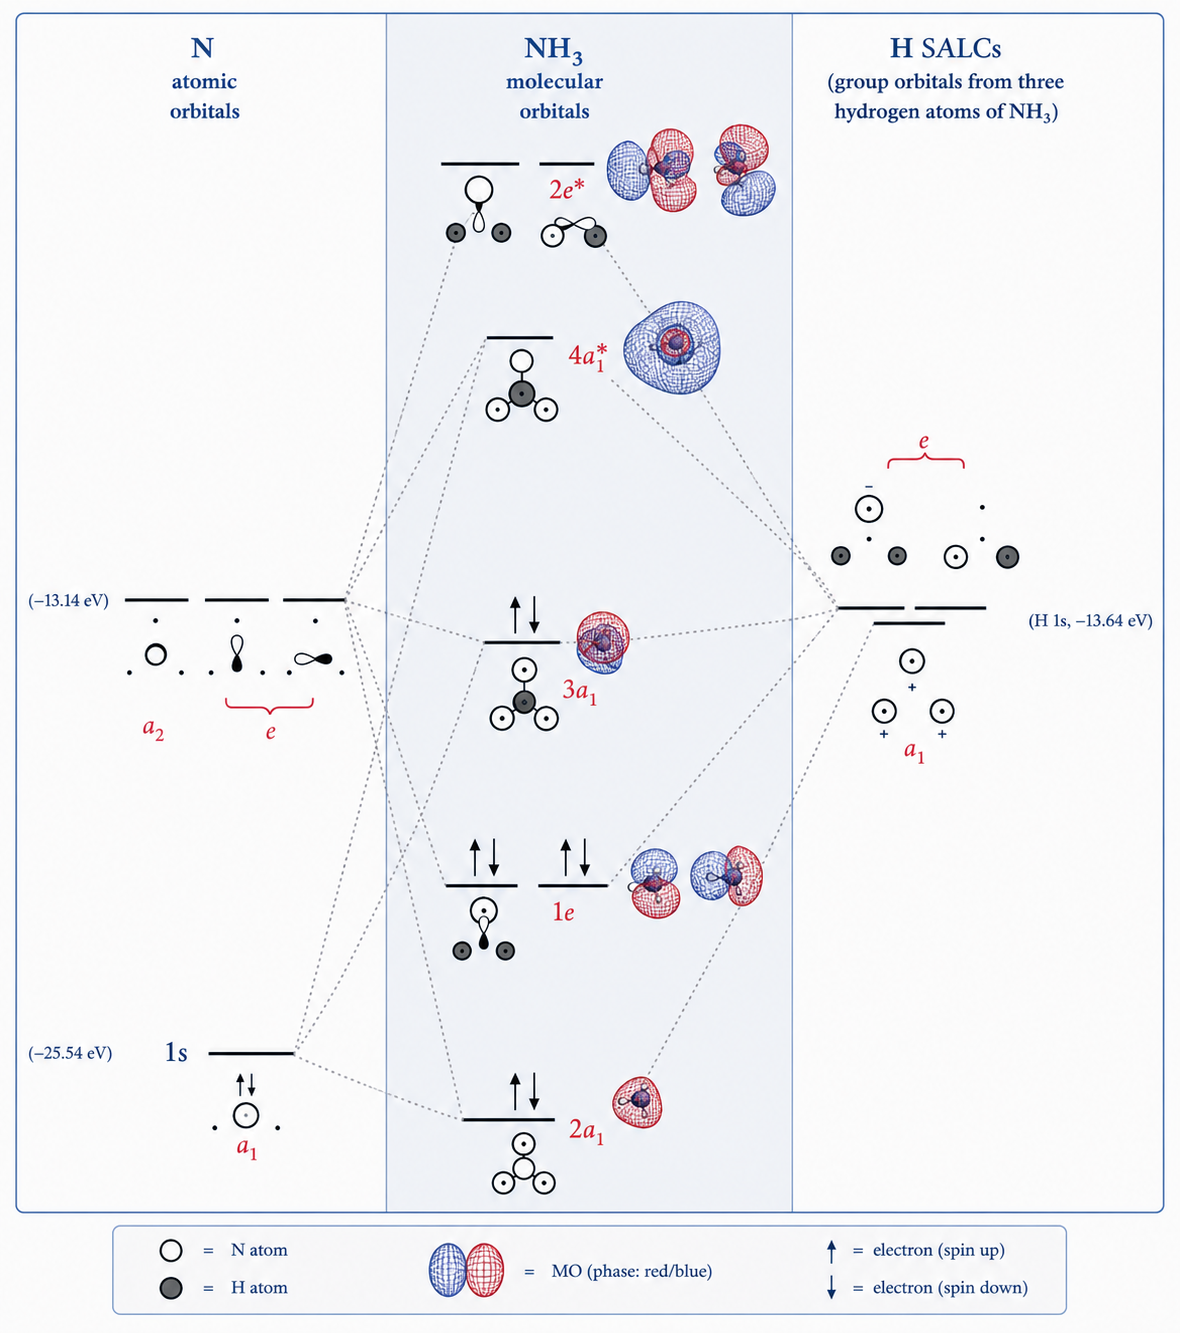
\includegraphics[keepaspectratio]{chapters/../images/image35.MO_NH3.png}}
\textbf{\emph{מסכנה:}} במקום לפתור בעיית \(7\times7\) (שלושה אורביטלי H
+ ארבעה של N), פותרים שתי בעיות קטנות: \(A_1\) (גודל \(3\times3\))
ו-\(E\) (גודל \(2\times2\) לכל כיוון). \#\# 5.8 חבורות מרחביות --- מבוא

עד כה עסקנו ב\textbf{חבורות נקודתיות} --- פעולות סימטריה של מולקולות
מבודדות, שכולן משמרות נקודה מרכזית.
\pandocbounded{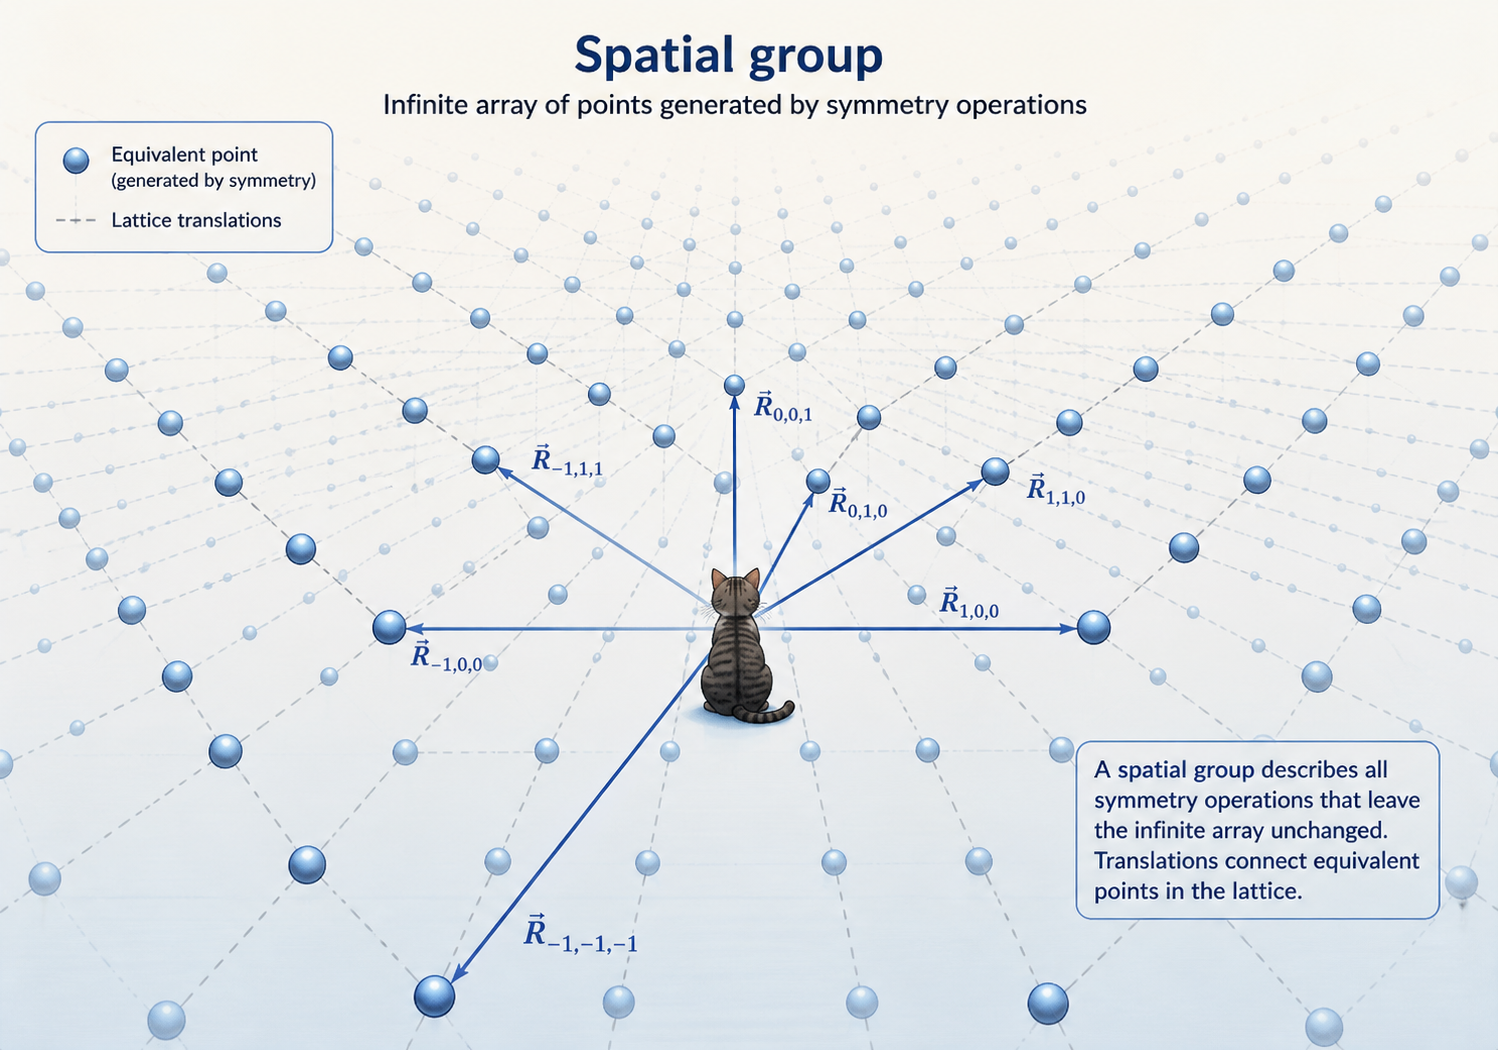
\includegraphics[keepaspectratio]{chapters/../images/image36.spaceGroups.png}}
בחומר מוצק, חוזרת יחידת הבנייה (תא יחידה) אינסוף פעמים בכל הכיוונים.
מוסיפים \textbf{טרנסלציות} (תזוזות) לפעולות הסימטריה, ומקבלים
\textbf{חבורות מרחביות} (space groups).

בתלת-ממד קיימות בדיוק \textbf{230 חבורות מרחביות} --- הוכח על ידי
הגאומטר הרוסי פדורוב (Fedorov) ב-1890. זה המספר הסופי האפשרי; אין יותר.

\textbf{אנלוגיה דו-ממדית:} כמה דרכים שונות סימטרית ניתן לכסות מישור
בתבנית חוזרת (כמו ריצוף)? בדיוק \textbf{17} --- \textbf{קבוצות טפטים}
(wallpaper groups). כל ריצוף שנפגשים בחיי יומיום שייך לאחת מ-17 הקבוצות
הללו.
\pandocbounded{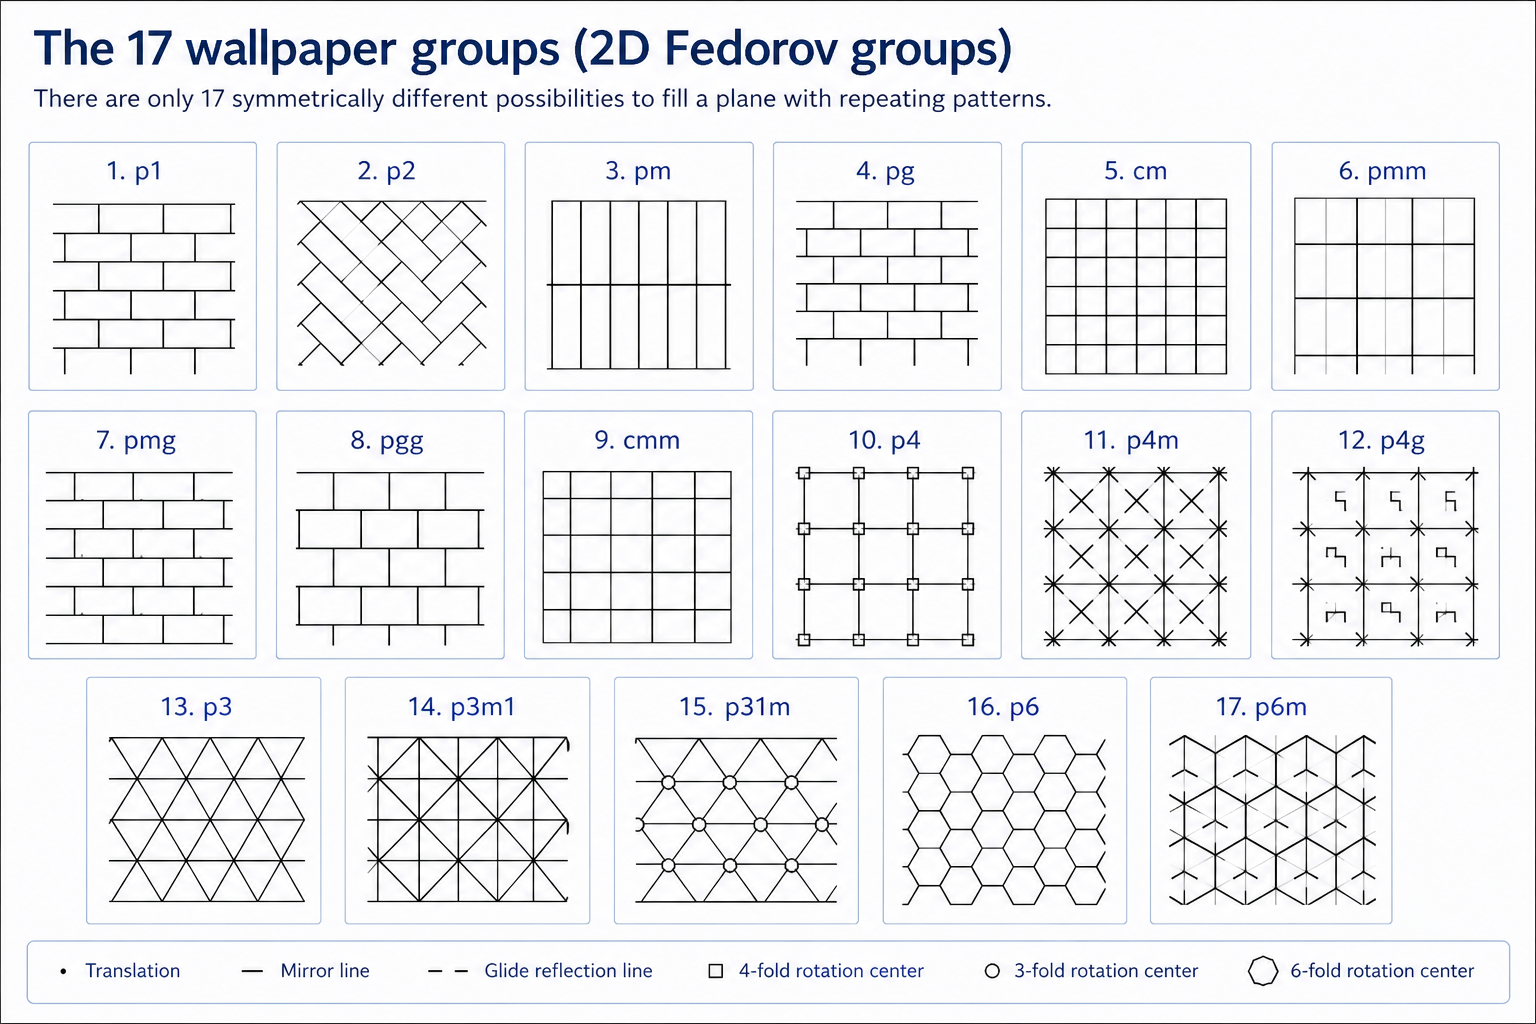
\includegraphics[keepaspectratio]{chapters/../images/image37.2Dwallpapers.png}}
\textbf{למנדס כימיה:} אינכם צריכים לשלוט ב-230 חבורות המרחב. אבל כאשר
תקראו מאמרים המתארים מבנה גבישי עם סימון כמו \(Fm\bar{3}m\) (זהו NaCl)
או \(P6_3/mmc\) (זהו גרפיט) --- אלו שמות חבורות מרחביות. כעת אתם יודעים
מה המשמעות. \#\# 5.9 מערכות גבישיות, סריגי ברווה וסימול פירסון\#\#

מערכות גבישיות (סינגוניות) כל המבנים הגבישיים מתחלקים לשבע מערכות
גבישיות (סינגוניות), המוגדרות על פי הקשרים בין אורכי צלעות תא היחידה (
\(a, b, c\)) והזוויות ביניהן (\(\alpha, \beta, \gamma\)):

\pandocbounded{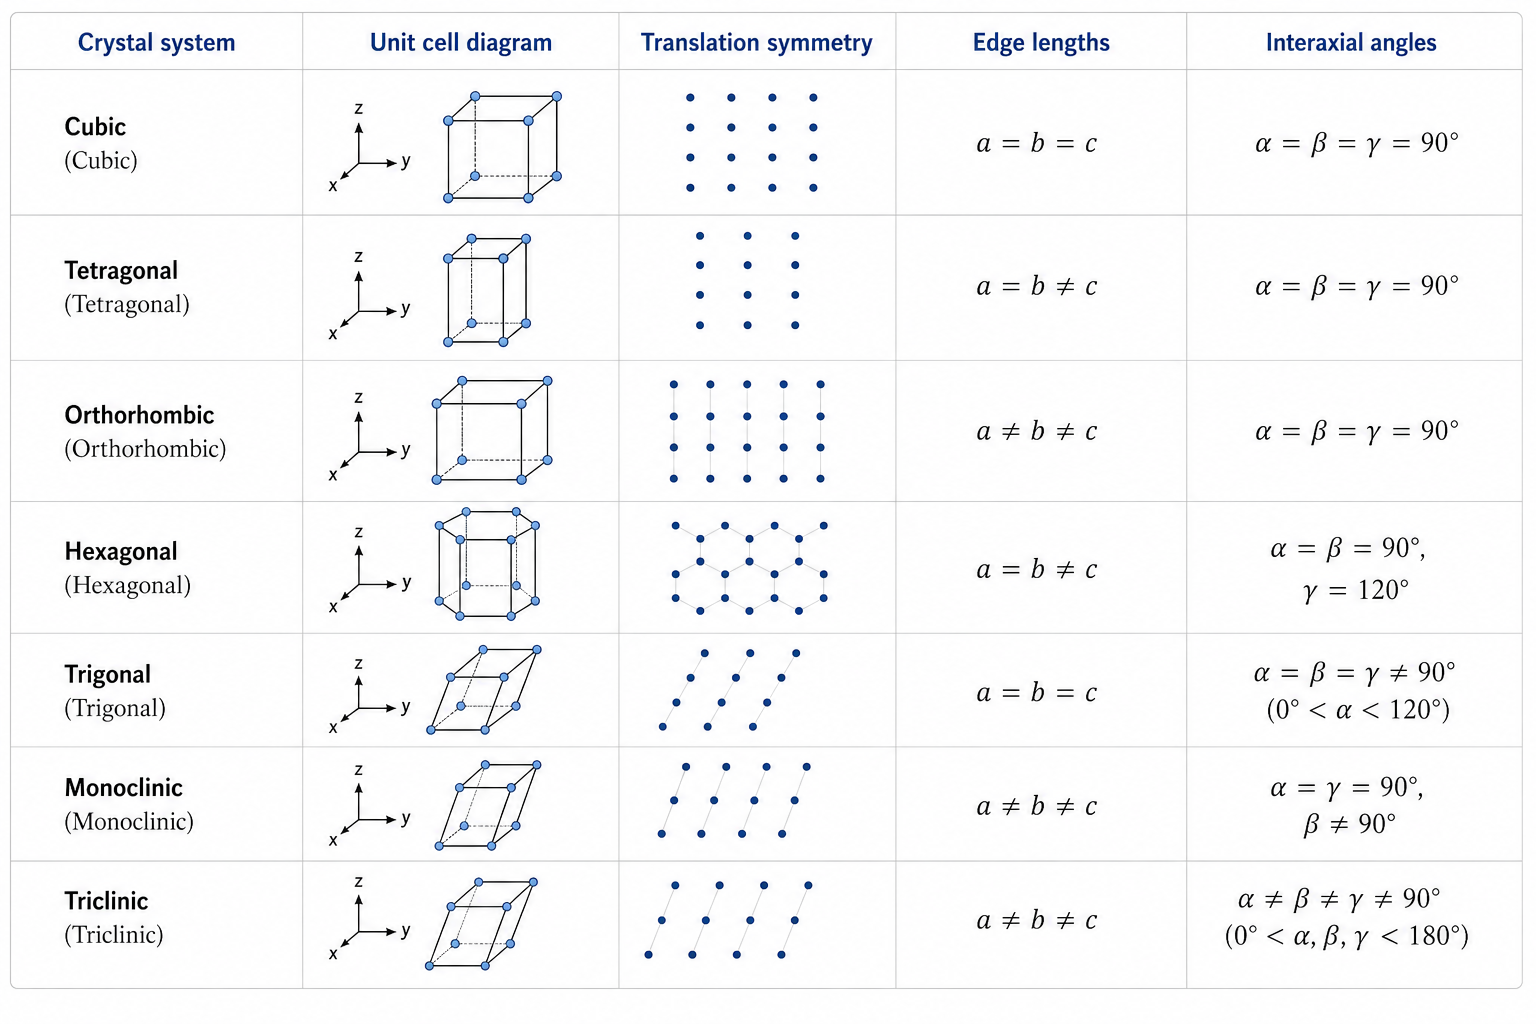
\includegraphics[keepaspectratio]{chapters/../images/image38.syngonias.png}}
הסינגוניה מגדירה את הסימטריה המינימלית של המבנה --- כלומר, את אילוצי
הגיאומטריה שחייבים להתקיים, לא את כל הסימטריה האפשרית.

\subsection{סוגי מירכוז (סוגי
סריג)}\label{ux5e1ux5d5ux5d2ux5d9-ux5deux5d9ux5e8ux5dbux5d5ux5d6-ux5e1ux5d5ux5d2ux5d9-ux5e1ux5e8ux5d9ux5d2}

בתוך כל סינגוניה ניתן למקם את נקודות הסריג בדרכים שונות. האפשרויות
השונות מכונות סוגי מירכוז (או סוגי סריג):

\pandocbounded{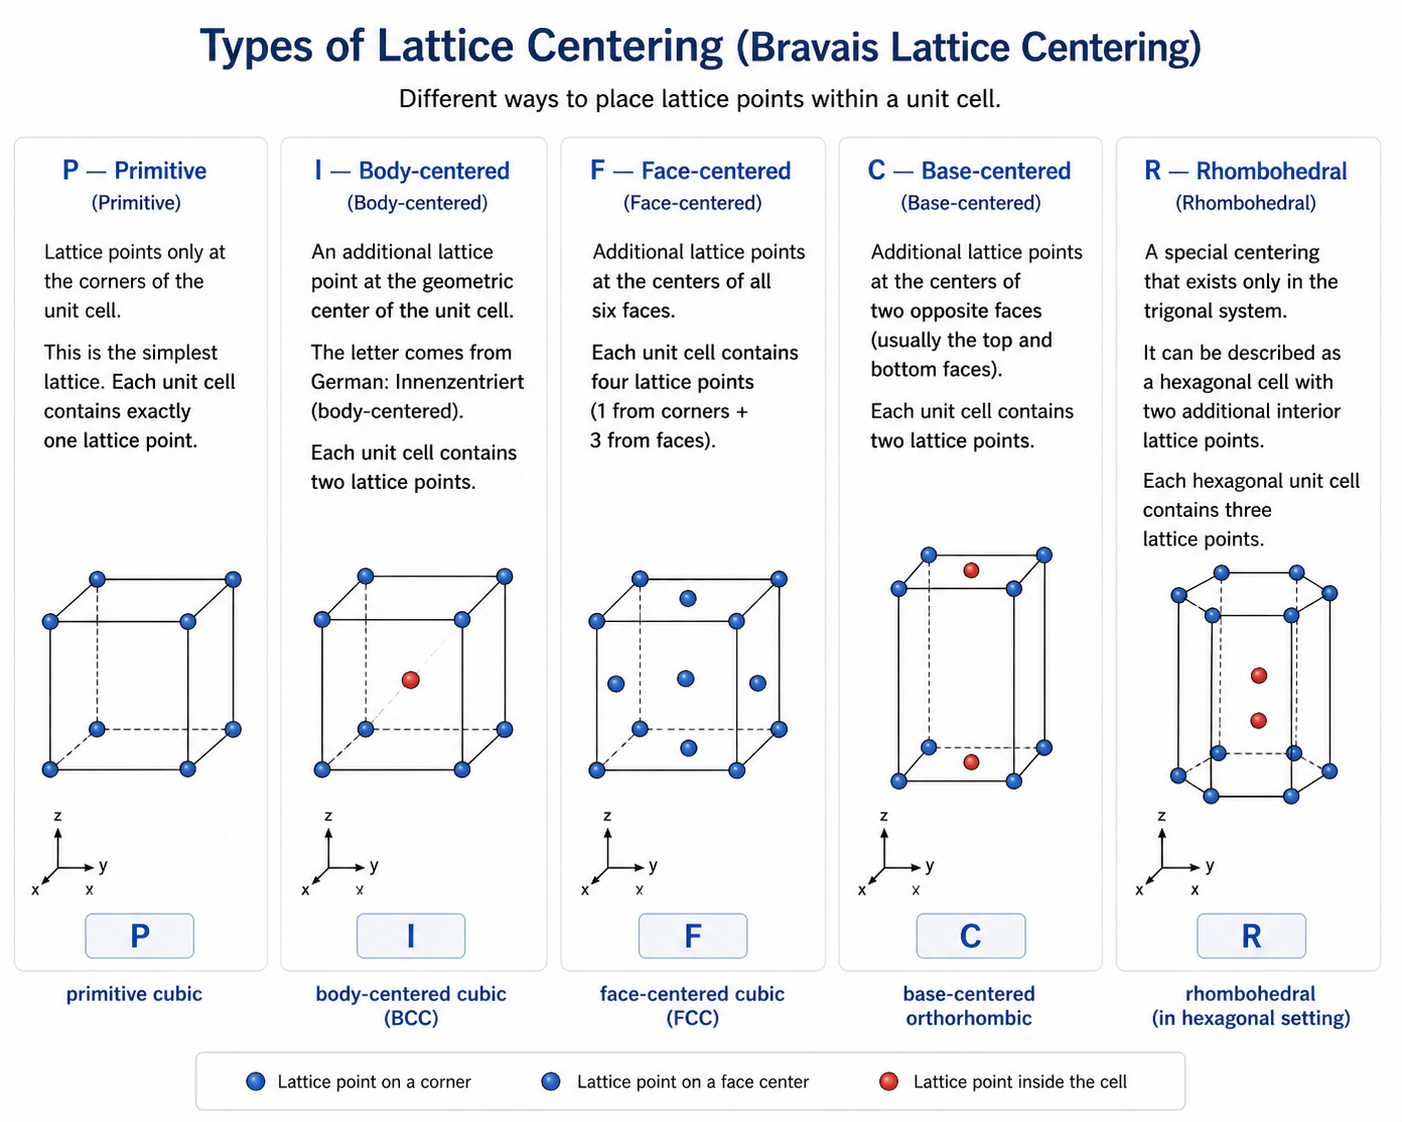
\includegraphics[keepaspectratio]{chapters/../images/image39.BravaisCentering.png}}

P --- פרימיטיבי (Primitive) --- נקודות סריג בפינות תא היחידה בלבד. זהו
הסריג הפשוט ביותר. לכל תא יחידה שייכת בדיוק נקודה אחת. I --- ממורכז בגוף
(Body-centered) --- נקודת סריג נוספת במרכז הגיאומטרי של תא היחידה. האות
מגיעה מגרמנית: Innenzentriert (ממורכז פנימית). לכל תא שייכות שתי נקודות.
F --- ממורכז בפיאות (Face-centered) --- נקודות סריג נוספות במרכז כל שש
הפיאות. לכל תא שייכות ארבע נקודות. C --- ממורכז בבסיס (Base-centered)
--- נקודות סריג נוספות רק במרכז שתי פיאות מקבילות (בדרך כלל הפיאות ).
לכל תא שייכות שתי נקודות. R --- רומבואדרי (Rhombohedral) --- מירכוז
מיוחד הקיים רק במערכת הטריגונלית. ניתן לתאר אותו כתא הכסגונלי עם שתי
נקודות פנימיות נוספות. לכל תא ההקסגונלי שייכות שלוש נקודות.

\subsection{סריגי
ברווה}\label{ux5e1ux5e8ux5d9ux5d2ux5d9-ux5d1ux5e8ux5d5ux5d5ux5d4}

השילוב בין שבע הסינגוניות וסוגי המירכוז האפשריים בכל אחת מהן נותן בדיוק
14 סריגי ברווה --- כל הצורות האפשריות לסידור תקופתי בתלת-מימד:
\pandocbounded{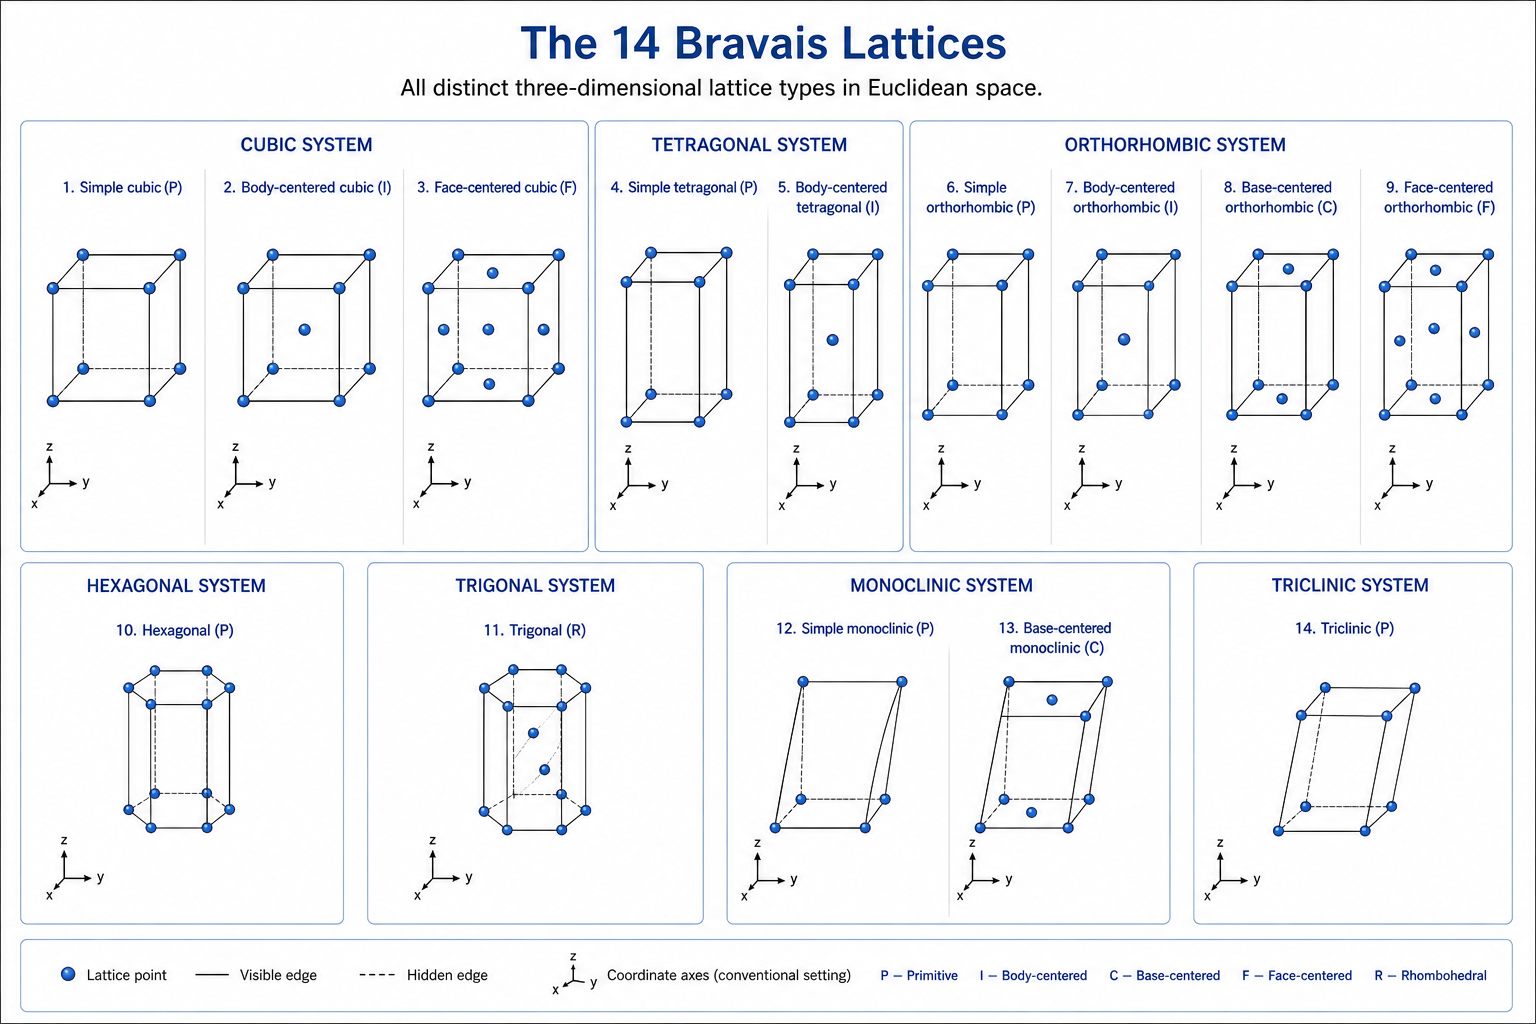
\includegraphics[keepaspectratio]{chapters/../images/image40.Bravais.png}}
שימו לב לשתי נקודות: ראשית, המערכת הטריגונלית מופיעה פעמיים --- היא
יכולה להיות מתוארת הן בסריג הכסגונלי (\emph{hP}) והן ברומבואדרי
(\emph{hR}), תלוי בגיאומטריה הספציפית. שנית, הסינגוניה האורתורומבית היא
העשירה ביותר --- ארבעה סריגים --- מכיוון שהיעדר אילוצים בין \(a\), \(b\)
ו-\(c\) מאפשר יותר אפשרויות מירכוז שאינן שקולות זו לזו.

\subsection{סימול
פירסון}\label{ux5e1ux5d9ux5deux5d5ux5dc-ux5e4ux5d9ux5e8ux5e1ux5d5ux5df}

לאחר שהבנו את הסריגים, סימול פירסון (Pearson) הופך לפשוט: הוא מקודד
שלושה פרטים גיאומטריים בשלושה תווים:

\begin{enumerate}
\def\labelenumi{\arabic{enumi}.}
\tightlist
\item
  \textbf{אות קטנה} --- מערכת גבישית: \(c\) (cubic), \(t\) (tetragonal),
  \(o\) (orthorhombic), \(h\) (hexagonal/trigonal), \(m\) (monoclinic),
  \(a\) (triclinic)
\item
  \textbf{אות גדולה} --- סוג הסריג: \(P\) (primitive), \(I\)
  (body-centered), \(F\) (face-centered), \(C\) (side-centered), \(R\)
  (rhombohedral)
\item
  \textbf{מספר} --- מספר האטומים בתא יחידה
\end{enumerate}

כלומר, סימול פירסון = סינגוניה + סוג סריג + תוכן תא היחידה. דוגמאות:
נחושת (Cu) גבישה ב-FCC: כל אטום זהה, 4 אטומים בתא ---
\pandocbounded{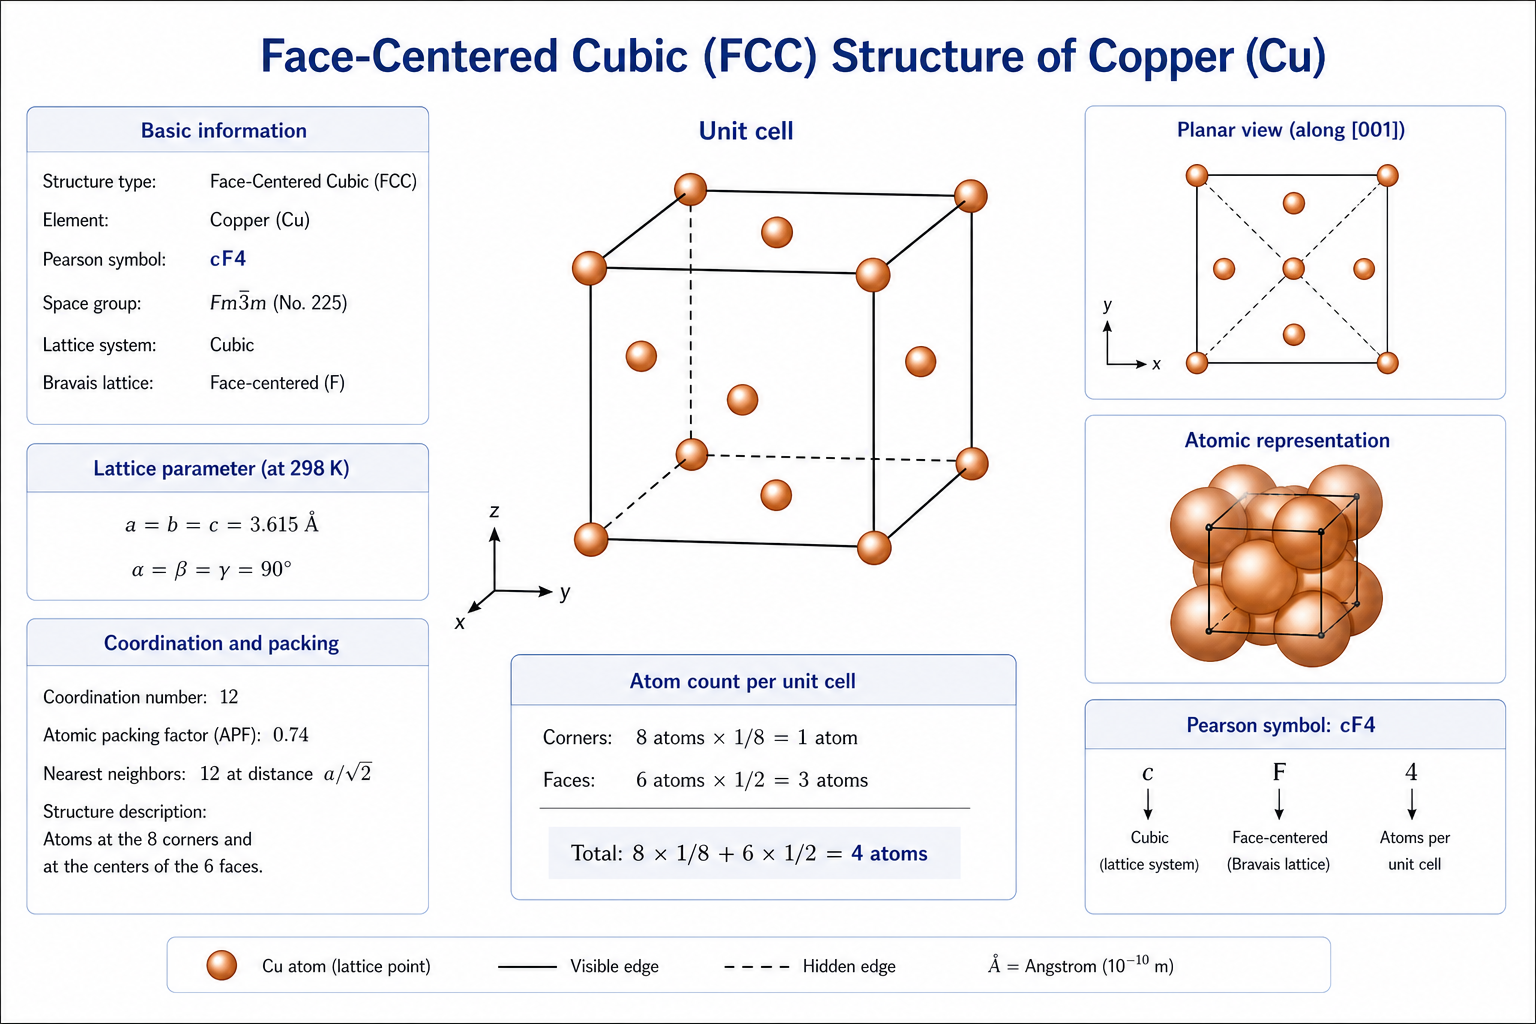
\includegraphics[keepaspectratio]{chapters/../images/image41.PearsonCu.png}}

נתרן (Na) גבישה ב-BCC: 2 אטומים בתא --- ברזל- (Fe) גם הוא BCC: --- אותו
סימול כמו Na, מכיוון שהגיאומטריה זהה. מלח בישול (NaCl): סריג FCC עם בסיס
של שני אטומים --- אטומים בתא --- יהלום (C): סריג FCC עם שני אטומי פחמן
בבסיס ---

\pandocbounded{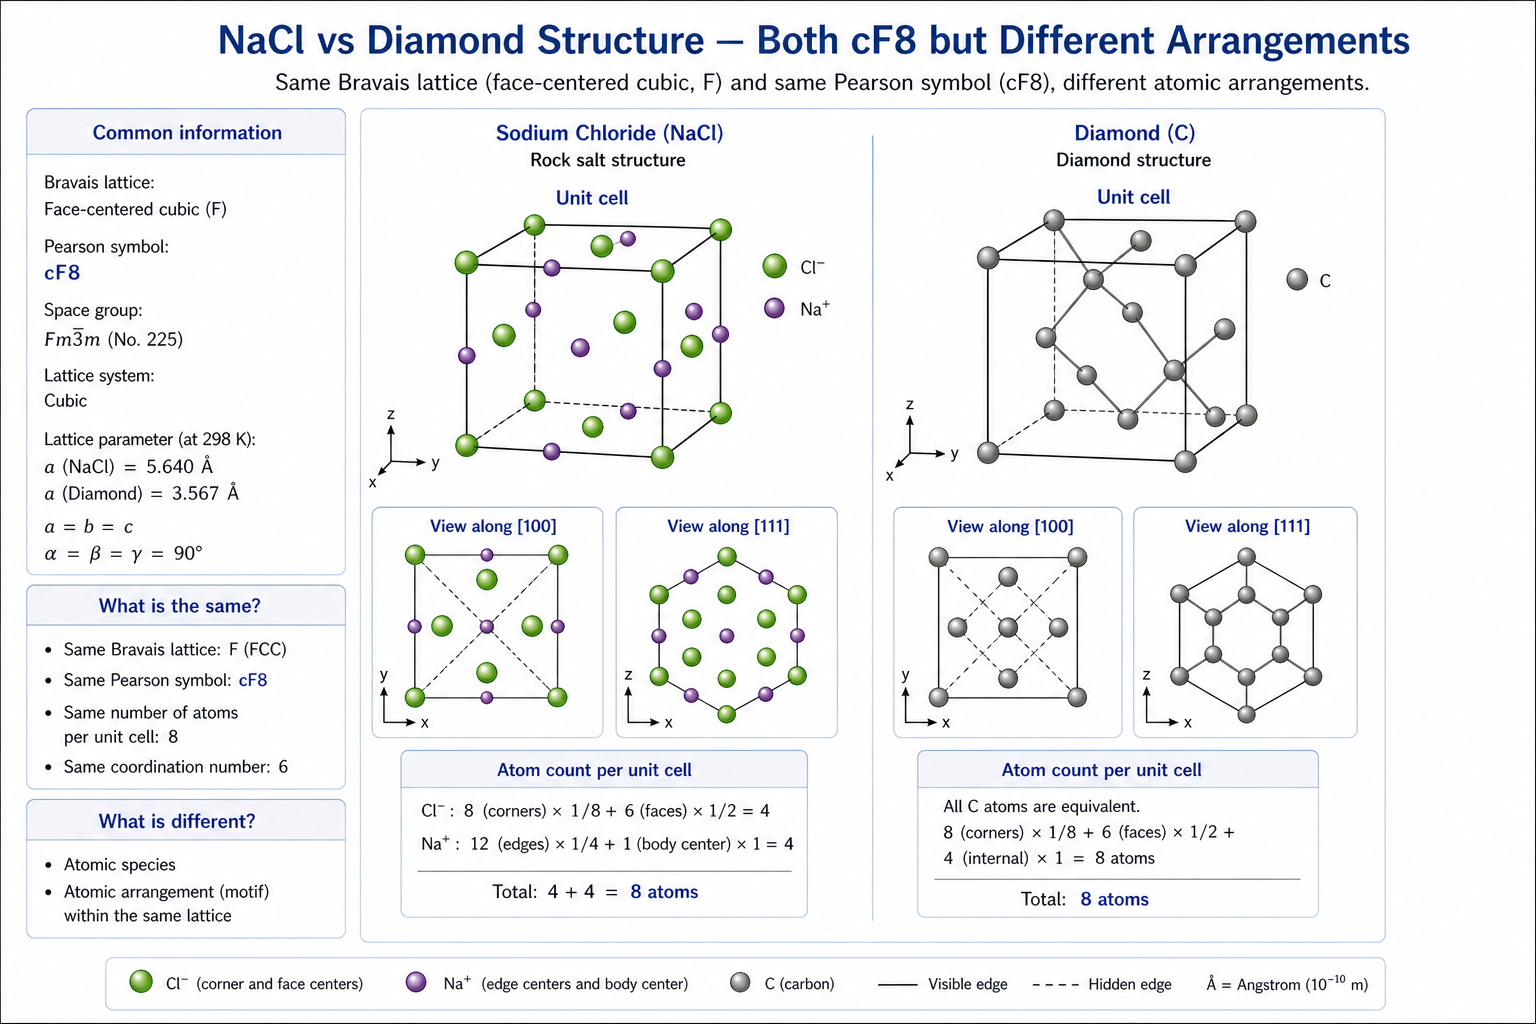
\includegraphics[keepaspectratio]{chapters/../images/image42.PearsonNaCl_C.png}}

וכאן מגיע המגבלה המהותית של סימול פירסון: NaCl ויהלום חולקים את אותו
סימול , אף על פי שמבניהם שונים לחלוטין --- ב-NaCl יש שני סוגי אטומים
הממוקמים בתתי-סריגים שונים, ביהלום יש אטום יחיד עם טטראהדרלי
קואורדינציה. הסימול מתאר סריג + כמות, אך לא סימטריה ולא מיקום האטומים
בתוך התא. כדי לתאר את המבנה במלואו --- כולל הסימטריה המלאה ומיקום כל
אטום --- נדרש כלי אחר: הקבוצה המרחבית וסימול הרמן-מוגן, אליו נעבור כעת.

\subsection{סימול הרמן-מוגן
(בינלאומי)}\label{ux5e1ux5d9ux5deux5d5ux5dc-ux5d4ux5e8ux5deux5df-ux5deux5d5ux5d2ux5df-ux5d1ux5d9ux5e0ux5dcux5d0ux5d5ux5deux5d9}

\subsubsection{שתי שפות לאותה סימטריה --- ולא
בדיוק}\label{ux5e9ux5eaux5d9-ux5e9ux5e4ux5d5ux5ea-ux5dcux5d0ux5d5ux5eaux5d4-ux5e1ux5d9ux5deux5d8ux5e8ux5d9ux5d4-ux5d5ux5dcux5d0-ux5d1ux5d3ux5d9ux5d5ux5e7}

סימול שנפליס (Schoenflies), שאיתו עבדנו עד כה, תוכנן לתאר \textbf{חבורה
נקודתית} --- סימטריה של אובייקט סופי: מולקולה, יון מתכת, גביש קטן.
הפעולות שמופיעות שם (סיבובים, שיקופים, היפוך) כולן משאירות לפחות נקודה
אחת במרחב קבועה.

גביש אמיתי הוא אחר. הוא אינסופי ומחזורי --- ויש לו פעולות סימטריה
שמערבות \textbf{תזוזה} (טרנסלציה). \textbf{ציר בורג} (screw axis) הוא
סיבוב בצירוף הזזה לאורך הציר. \textbf{מישור החלקה} (glide plane) הוא
שיקוף בצירוף הזזה במישור. שתי הפעולות האלה אינן קיימות כלל בסימול שנפליס
--- לא מפני שנשכחו, אלא מפני שהן פשוט אינן רלוונטיות לאובייקט סופי.

זו הסיבה ל-230 חבורות מרחביות (space groups) לעומת 32 קבוצות נקודתיות
בלבד: כל קבוצה נקודתית ``מתפצלת'' למספר קבוצות מרחביות שונות, בהתאם
לאופן שבו משלבים בה פעולות טרנסלציוניות.
\pandocbounded{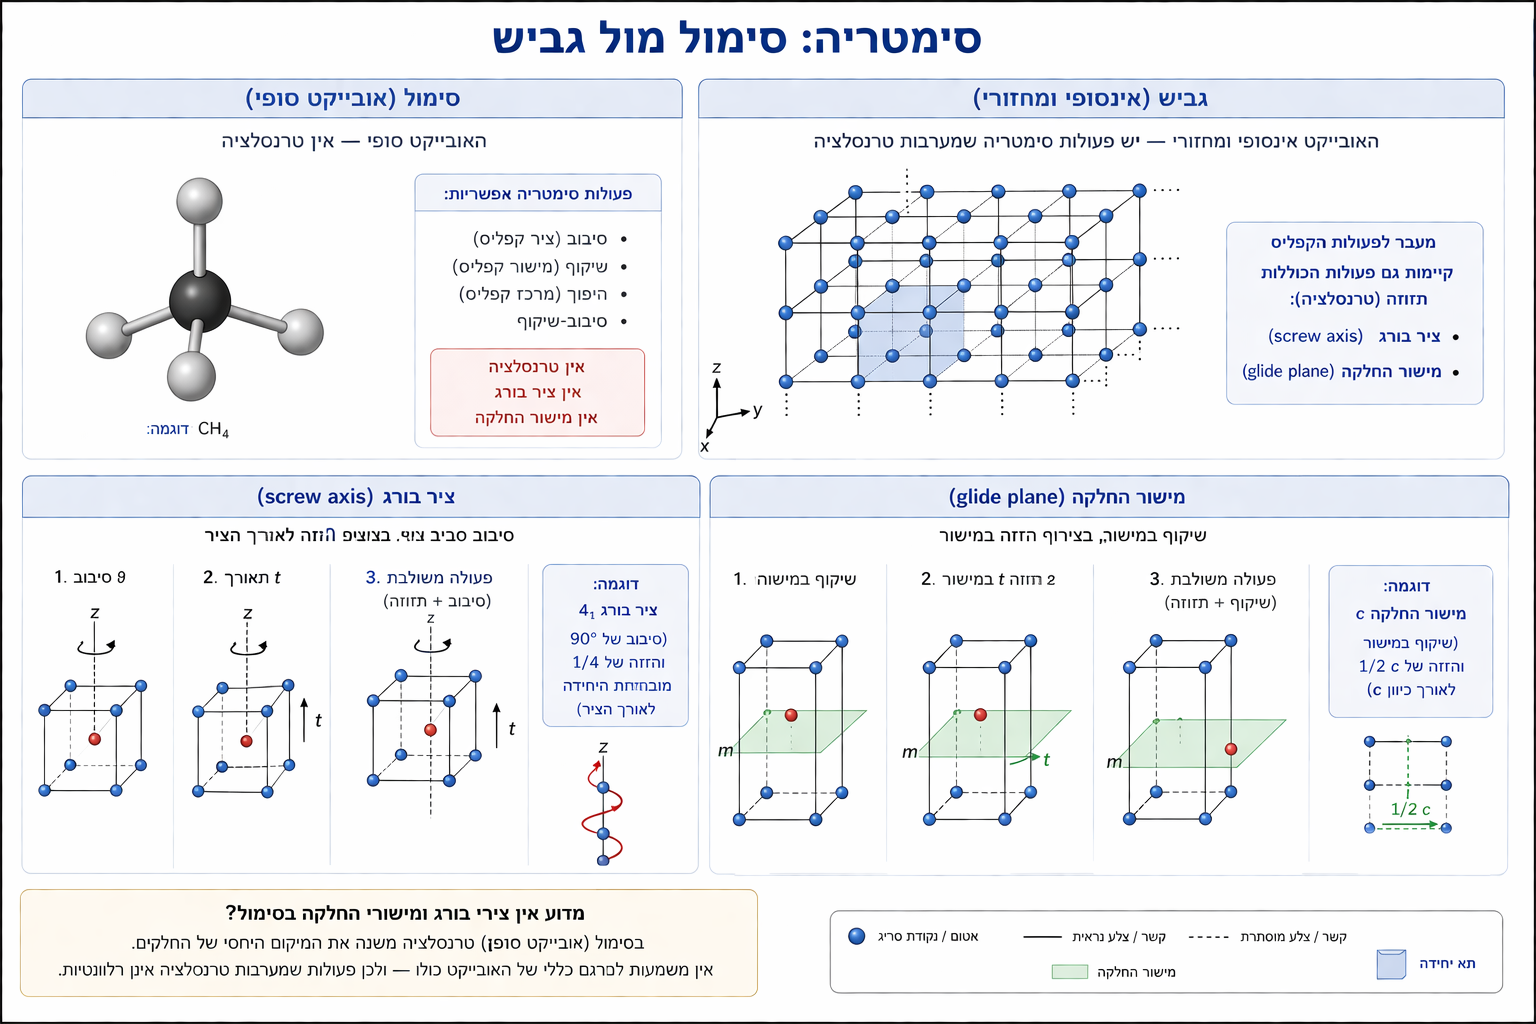
\includegraphics[keepaspectratio]{chapters/../images/image43.HermannMaugin.png}}
סימול הרמן-מוגן תוכנן מלכתחילה עבור הקבוצות המרחביות. הוא מתאר לא רק את
הסימטריה של הנקודה, אלא את הסימטריה של כל המבנה התקופתי. \#\#\#\#
מהשנפליס להרמן-מוגן: ``תרגום'' ומגבלותיו

במקרים רבים ניתן לעבור מסימול שנפליס לסימול הרמן-מוגן באופן ישיר.
לדוגמה:

{\def\LTcaptype{none} % do not increment counter
\begin{longtable}[]{@{}ll@{}}
\toprule\noalign{}
שנפליס & הרמן-מוגן (חברוה נקודתית) \\
\midrule\noalign{}
\endhead
\bottomrule\noalign{}
\endlastfoot
\(C_1\)\hspace{0pt} & 1 \\
\(C_2\) & 1 \\
\(C_s\)\hspace{0pt} & m \\
\(C_{2h}\)\hspace{0pt} & 2/m \\
\(D_{2h}\)\hspace{0pt} & mmm \\
\(T_d​\) & \(\bar{4}3m\) \\
\(O_h\) & \(m\bar{3}m\) \\
\(C_{3v}\) & \emph{3m} \\
\(D_{6h} ​\) & \emph{6/mmm } \\
\end{longtable}
}

הסימטריה עצמה זהה --- רק השפה שונה. ה-``תרגום'' עובד כאשר מדברים על
\textbf{חבורה נקודתית} בלבד, אך ברגע שעוברים לחבורות \textbf{מרחביות},
התרגום הפשוט נשבר. לחבורה נקודתית \emph{mmm} = \(D_{2h}\) \hspace{0pt}יש
28 חבורות מרחביות שונות --- ביניהן \emph{Pmmm} ,\emph{Pbca}, \emph{Cmce}
ואחרות --- כל אחת עם שילוב שונה של מישורי החלקה וצירי בורג. \#\#\#\#
הבדל מושגי אחד: היפוך לעומת סיבוב מדומה לפני שממשיכים, יש להבהיר הבדל
טכני אחד בין שתי השיטות --- שיכול לגרום לבלבול. שנפליס משתמש
ב\textbf{סיבובמדומה} (\(S_n\)\hspace{0pt}): סיבוב בזווית
\(\frac{360^\circ}{n}\) ואחריו שיקוף במישור הניצב לציר.
לדוגמה,\(S_2\)\hspace{0pt} --- סיבוב ב-180° ושיקוף (שווה ערך
לאינוורסיה).

הרמן-מוגן משתמש ב\textbf{ציר אינוורסיה} (\(\bar{n}\)): סיבוב בזווית
\(\frac{360^\circ}{n}\)\hspace{0pt} ואחריו אינוורסיה דרך נקודה. התוצאה
דומה, אך לא זהה תמיד:
\(S_2 = \bar{1}, \quad S_4 = \bar{4}, \quad S_6 = \bar{3}\)

אך \(S_3 \neq \bar{3}\) ו-\(S_6 \neq \bar{6}\) --- כלומר, עבור n מסוים
שתי השיטות מייצרות פעולות שונות. בפועל, ברוב המקרים שתיראו בקורס ניתן
לעבור ישירות מהטבלה. אך חשוב לדעת שההבדל קיים. \#\# סימול
Hermann-Mauguin (בינלאומי)

סימול הרמן-מוגן מורכב מארבעה חלקים:

\begin{enumerate}
\def\labelenumi{\arabic{enumi}.}
\tightlist
\item
  מרכוז הסריג: \(P\), \(I\), \(F\), \(A/B/C\), \(R\) 2--4. פעולות
  הסימטריה לאורך שלושה כיווני סימטריה ראשיים
\end{enumerate}

דוגמה --- קוורץ (\(\alpha\)-SiO₂): \(P3_1 2_1\)

\begin{itemize}
\tightlist
\item
  \(P\) = פרימיטיבי
\item
  \(3_1\) = ציר בורג תלת-סדרי (סיבוב ב-120° + תזוזה של \(\frac{1}{3}\)
  פרמטר תא)
\item
  \(2_1\) = ציר בורג דו-סדרי
\end{itemize}

הסימנים לפעולות הסימטריה:

\begin{itemize}
\tightlist
\item
  \(n\) --- ציר סיבוב מסדר \(n\) (כגון 2, 3, 4, 6)
\item
  \(\bar{n}\) --- ציר אינוורסיה מסדר \(n\)
\item
  \(m\) --- מישור שיקוף (mirror)
\item
  \(n/m\) --- ציר סיבוב עם מישור שיקוף ניצב
\item
  \(n_p\) --- ציר בורג (למשל \(2_1\), \(3_1\), \(4_2\) וכו')
\item
  \(a, b, c, n, d\) --- מישורי החלקה
\item
  \(1\) --- אין סימטריה (זהות)
\end{itemize}

מישורי ההחלקה מציינים תזוזה של \(\frac{1}{2}a\), \(\frac{1}{2}b\),
\(\frac{1}{2}c\) לאורך אלכסון, \(\frac{1}{4}\) לאורך אלכסון, בהתאמה.
\#\#\# פעולות חדשות: צירי בורג ומישורי החלקה
\pandocbounded{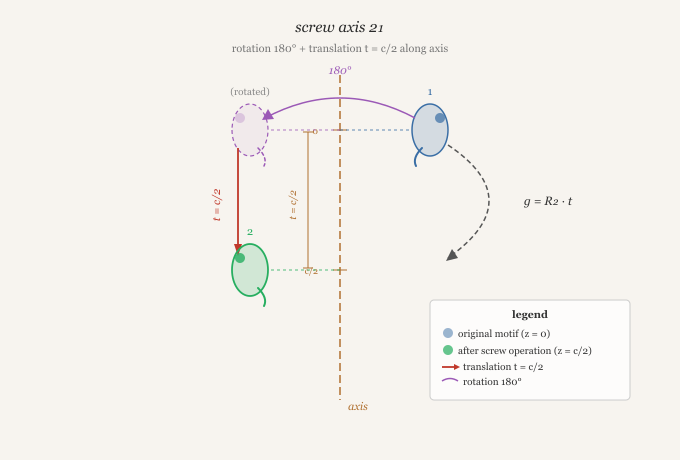
\includegraphics[keepaspectratio]{chapters/../images/image44.ScrewAxis.png}}

\textbf{ציר בורג \(n_p\)} --- סיבוב ב-\(\frac{360°}{n}\) בצירוף הזזה של
\(\frac{p}{n}\) פרמטר תא לאורך הציר. ציר \(2_1\) פירושו: סיבוב ב-180° +
הזזה של \(\frac{1}{2}c\). ציר \(4_1\) פירושו: סיבוב ב-90° + הזזה של
\(\frac{1}{4}c\).

שימו לב: לאחר \(n\) פעמים חוזרים לנקודת המוצא (כולל טרנסלציה של פרמטר תא
שלם) --- לכן מדובר בפעולת סימטריה לגיטימית של המבנה התקופתי.

\pandocbounded{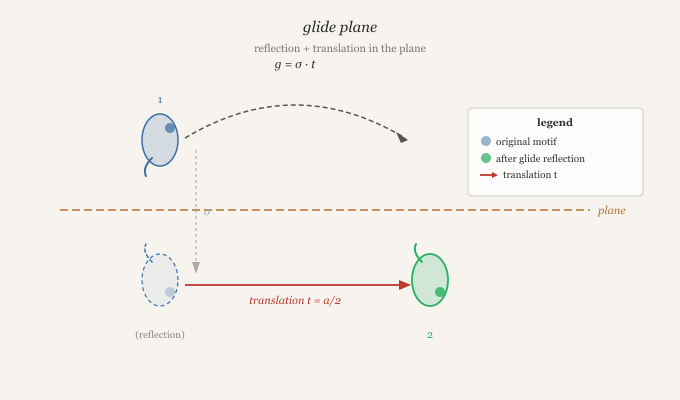
\includegraphics[keepaspectratio]{chapters/../images/image45.GlideReflection.png}}

\textbf{מישור החלקה} --- שיקוף במישור בצירוף הזזה של חצי פרמטר תא
\textbf{בתוך} המישור. אם ההזזה היא לאורך \(a\), קוראים למישור
\(a\)-glide; לאורך \(b\) --- \(b\)-glide; וכן הלאה. \#\#\# הכיוונים
הראשיים לפי סינגוניה

שלוש עמדות הסימול מתאימות לכיוונים שונים בהתאם לסינגוניה. זו הנקודה
שדורשת שימת לב --- אותה עמדה יכולה לתאר כיוון שונה לחלוטין במערכת שונה.

\textbf{מערכת קובית:}

{\def\LTcaptype{none} % do not increment counter
\begin{longtable}[]{@{}ll@{}}
\toprule\noalign{}
עמדה & כיוון \\
\midrule\noalign{}
\endhead
\bottomrule\noalign{}
\endlastfoot
1 & \(\langle 100 \rangle\) --- הצלעות \\
2 & \(\langle 111 \rangle\) --- האלכסונים המרחביים \\
3 & \(\langle 110 \rangle\) --- האלכסונים של הפיאות \\
\end{longtable}
}

דוגמה: \(Fm\bar{3}m\) (נחושת, זהב, NaCl מבחינת הסריג) --- \(F\) = ממורכז
בפיאות, \(m\) = מישור שיקוף לאורך \(\langle 100 \rangle\), \(\bar{3}\) =
ציר אינוורסיה תלת-סדרי לאורך \(\langle 111 \rangle\), \(m\) = מישור
שיקוף לאורך \(\langle 110 \rangle\).

\textbf{מערכת הקסגונלית:}

{\def\LTcaptype{none} % do not increment counter
\begin{longtable}[]{@{}ll@{}}
\toprule\noalign{}
עמדה & כיוון \\
\midrule\noalign{}
\endhead
\bottomrule\noalign{}
\endlastfoot
1 & \([001]\) --- ציר \(c\) (ציר הסימטריה הראשי) \\
2 & \(\langle 100 \rangle\) --- הצלעות של הבסיס ההקסגונלי \\
3 & \(\langle 110 \rangle\) --- האלכסונים של הבסיס ההקסגונלי \\
\end{longtable}
}

\pandocbounded{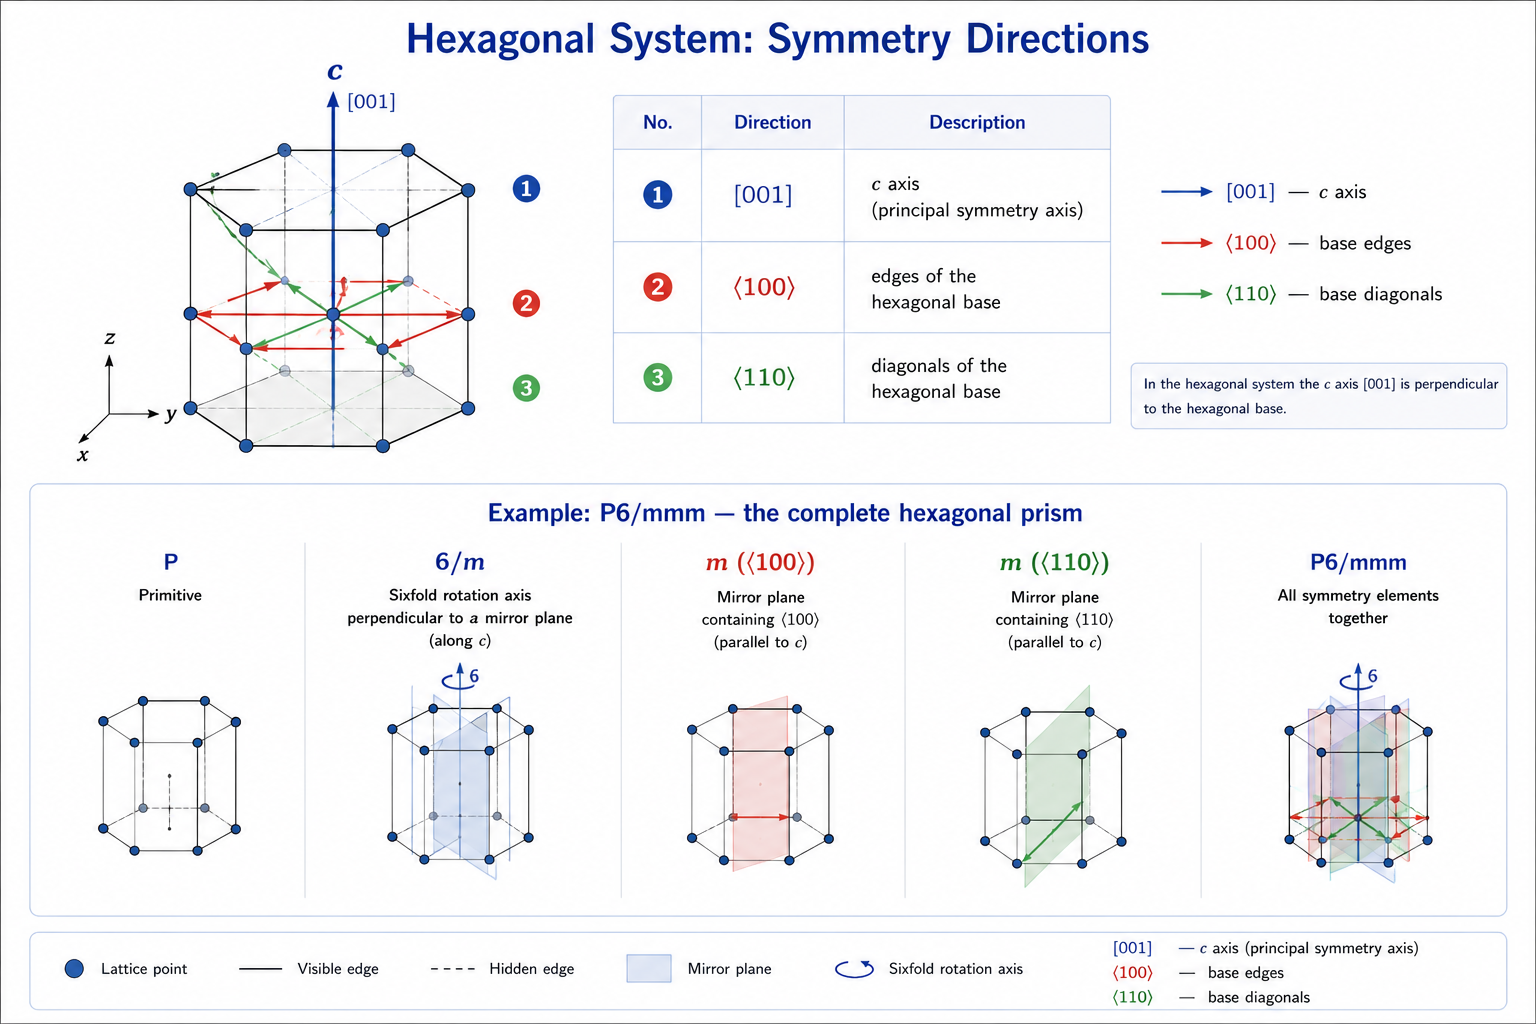
\includegraphics[keepaspectratio]{chapters/../images/image46.hexagonal.png}}

דוגמה: \(P6/mmm\) --- הפריסמה ההקסגונלית המלאה. \(P\) = פרימיטיבי,
\(6/m\) = ציר שישי-סדרי ניצב למישור שיקוף (לאורך \(c\)), \(m\) = שיקוף
לאורך \(\langle 100 \rangle\), \(m\) = שיקוף לאורך
\(\langle 110 \rangle\).

דוגמה עם ציר בורג --- קוורץ (\(\alpha\)-SiO₂): \(P3_121\) --- \(P\) =
פרימיטיבי, \(3_1\) = ציר בורג תלת-סדרי לאורך \(c\), \(2\) = ציר דו-סדרי
לאורך \(\langle 100 \rangle\), \(1\) = אין סימטריה לאורך
\(\langle 110 \rangle\).

\pandocbounded{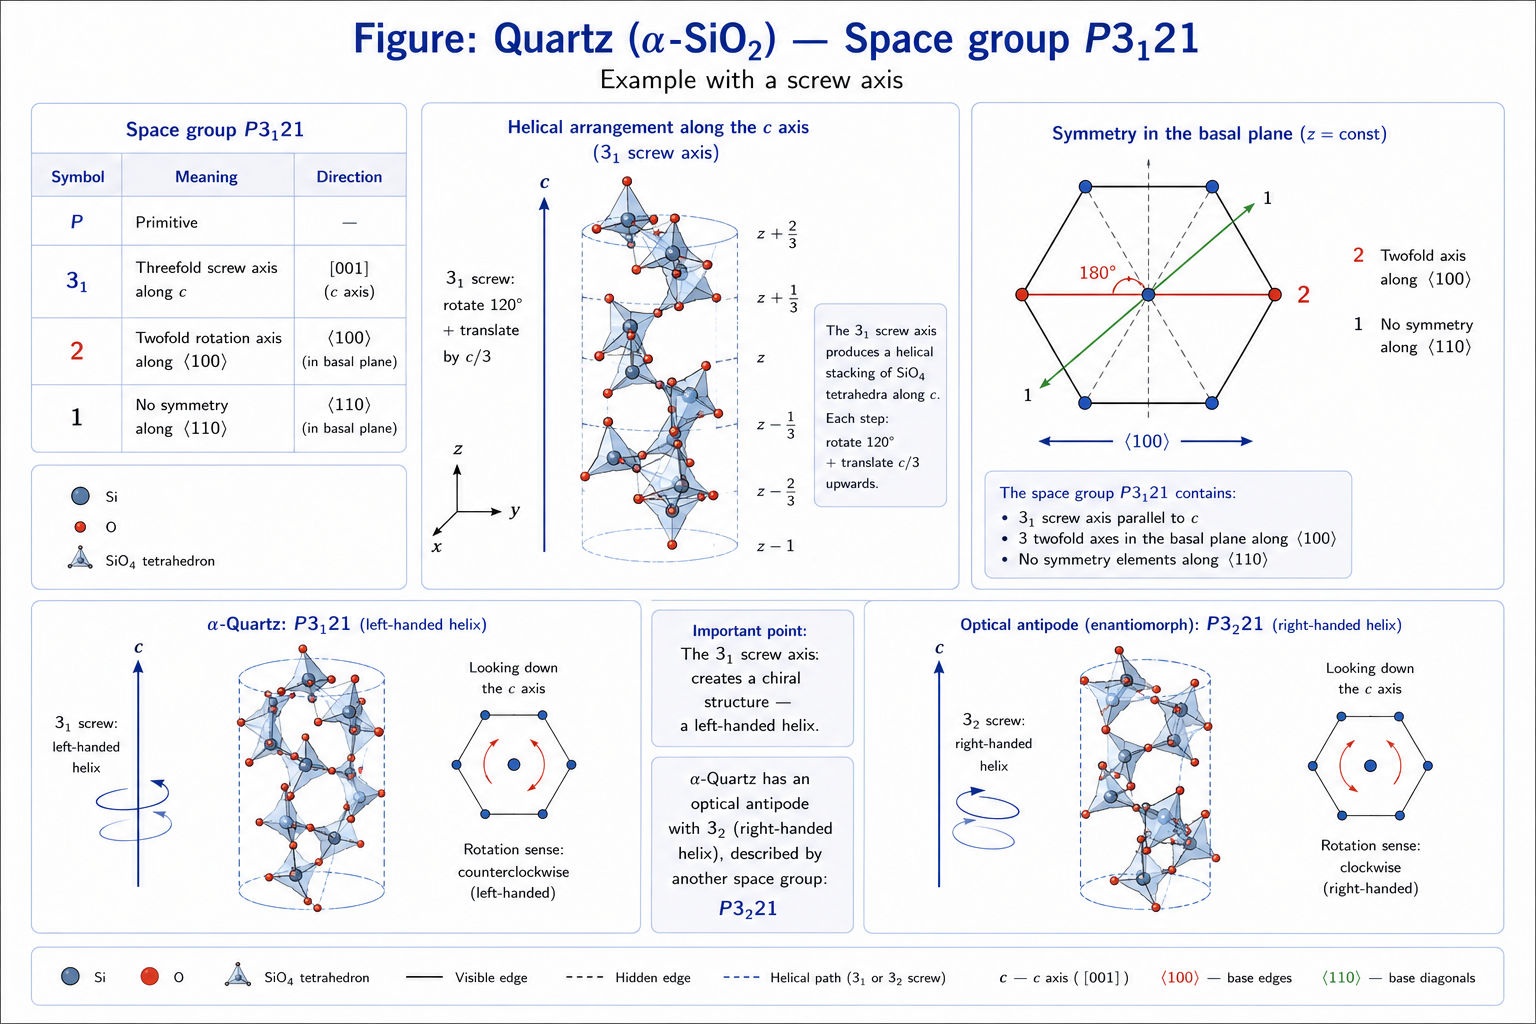
\includegraphics[keepaspectratio]{chapters/../images/image47.quartz.png}}

הקוורץ מדגים נקודה חשובה: ציר הבורג \(3_1\) יוצר מבנה \textbf{כירלי} ---
סליל שמאלי. ל-\(\alpha\)-קוורץ יש אנטיפוד אופטי עם \(3_2\) (סליל ימני),
המתואר על ידי קבוצה מרחבית אחרת: \(P3_221\). \#\#\# טבלת השוואה מסכמת

{\def\LTcaptype{none} % do not increment counter
\begin{longtable}[]{@{}
  >{\raggedright\arraybackslash}p{(\linewidth - 4\tabcolsep) * \real{0.3333}}
  >{\raggedright\arraybackslash}p{(\linewidth - 4\tabcolsep) * \real{0.3333}}
  >{\raggedright\arraybackslash}p{(\linewidth - 4\tabcolsep) * \real{0.3333}}@{}}
\toprule\noalign{}
\begin{minipage}[b]{\linewidth}\raggedright
מאפיין
\end{minipage} & \begin{minipage}[b]{\linewidth}\raggedright
שנפליס
\end{minipage} & \begin{minipage}[b]{\linewidth}\raggedright
הרמן-מוגן
\end{minipage} \\
\midrule\noalign{}
\endhead
\bottomrule\noalign{}
\endlastfoot
מתאר & קבוצות נקודה & קבוצות נקודה וקבוצות מרחביות \\
מספר הקבוצות & 32 & 32 (נקודה) + 230 (מרחבי) \\
פעולות עם טרנסלציה & לא & כן (צירי בורג, מישורי החלקה) \\
שימוש עיקרי & ספקטרוסקופיה, כימיה קוונטית & קריסטלוגרפיה, מסדי נתונים
גבישיים \\
סימן לאינוורסיה & \(S_{2n}\) & \(\bar{n}\) \\
\end{longtable}
}

הדבר האחרון שחסר לתיאור מלא של מבנה גבישי הוא מיקום האטומים
\textbf{בתוך} תא היחידה --- ה\textbf{מיקום של ויקוף} (Wyckoff position),
אך זה כבר נושא לפרק הבא. \#\# סיכום

ארבעה נושאים עיקריים בפרק:

\textbf{פעולות סימטריה} --- חמישה סוגים: \(E\), \(C_n\), \(\sigma\),
\(i\), \(S_n\). כל אחד מוגדר על ידי האלמנט הגיאומטרי שלו.

\textbf{חבורות נקודה} --- אוסף כל פעולות הסימטריה של מולקולה. קיימות 32
חבורות נקודה; כל מולקולה שייכת לאחת מהן.

\textbf{טבלאות כרקטרים} --- מסכמות את תכונות החבורה בצורה קומפקטית.
כרקטר = מספר האטומים שלא זזו = טרייס המטריצה.

\textbf{SALCs} --- קומבינציות מותאמות-סימטריה של אורביטלים אטומיים.
מאפשרות לבנות אורביטלים מולקולריים בשיטה שיטתית תוך צמצום דרמטי של
מורכבות החישוב. רק אורביטלים מאותה הצגה מתחברים.

\bookmarksetup{startatroot}

\chapter{פרק 6 --- מבנה מולקולרי: קשרים, היברידיזציה
וספקטרוסקופיה}\label{ux5e4ux5e8ux5e7-6-ux5deux5d1ux5e0ux5d4-ux5deux5d5ux5dcux5e7ux5d5ux5dcux5e8ux5d9-ux5e7ux5e9ux5e8ux5d9ux5dd-ux5d4ux5d9ux5d1ux5e8ux5d9ux5d3ux5d9ux5d6ux5e6ux5d9ux5d4-ux5d5ux5e1ux5e4ux5e7ux5d8ux5e8ux5d5ux5e1ux5e7ux5d5ux5e4ux5d9ux5d4}

\section{מבוא: שלוש שפות לתיאור קשר
כימי}\label{ux5deux5d1ux5d5ux5d0-ux5e9ux5dcux5d5ux5e9-ux5e9ux5e4ux5d5ux5ea-ux5dcux5eaux5d9ux5d0ux5d5ux5e8-ux5e7ux5e9ux5e8-ux5dbux5d9ux5deux5d9}

קשר כימי מתואר על ידי שתי תיאוריות מרכזיות: \textbf{תיאוריית קשרי
הערכיות (Valence Bond, VB)} --- האינטואיטיבית יותר: אלקטרונים בעלי
ספינים מנוגדים ``מזדווגים'' ויוצרים קשר. במסגרתה פועלים שני כלים
משלימים: \textbf{\emph{דחיית זוגות טלרטרוני הערכיות, Valence Shell
Electrone Pair Repulsion, VSEPR ---}} לניבוי הגיאומטריה על פי דחיית
זוגות האלקטרונים --- ו\textbf{\emph{היברידיזציה}}, המשלבת את שניהם
לתיאור מקיף של הקשר והצורה.

\textbf{תיאוריית האורביטלים המולקולריים (Molecular Orbital, MO)} ---
המדויקת יותר אך פחות אינטואיטיבית: אורביטלים אטומיים מתחברים לאורביטלים
המשותפים לכל המולקולה. SALCs שבנינו בפרק הקודם הן הבסיס לגישה זו.

שתי התיאוריות נכונות ומשלימות זו את זו. פרק זה יציג אותן ויסביר מתי
להשתמש בכל אחת. \#\# 6.1 מומנט דיפול --- מדד הפולריות

\subsection{מהו דיפול?}\label{ux5deux5d4ux5d5-ux5d3ux5d9ux5e4ux5d5ux5dc}

כאשר צפיפות האלקטרונים במולקולה אינה מפולגת בצורה אחידה --- יש
\textbf{הפרדת מטען} בין חלק חיובי וחלק שלילי. מצב זה נקרא \textbf{דיפול}
(dipole, מיוונית ולטינית ``שני קטבים'').

\textbf{מומנט הדיפול} הוא וקטור המכמת הפרדה זו:

\[\vec{\mu} = \sum_i q_i \vec{r}_i\]

כאשר \(q_i\) הוא המטען של חלקיק \(i\) ו-\(\vec{r}_i\) הוא מיקומו. מומנט
הדיפול נמדד ביחידות \textbf{דביי} (D):
\(1;\text{D} = 3.33 \times 10^{-30};\text{C·m}\).

\subsection{מה קובע את מומנט
הדיפול?}\label{ux5deux5d4-ux5e7ux5d5ux5d1ux5e2-ux5d0ux5ea-ux5deux5d5ux5deux5e0ux5d8-ux5d4ux5d3ux5d9ux5e4ux5d5ux5dc}

שני גורמים: \textbf{הפרש האלקטרושליליות} בין האטומים (כמה חזק כל אטום
מושך אל עצמו אלקטרונים), \textbf{וסימטריית המולקולה} (האם הדיפולים
מבטלים זה את זה, חלקית או לחלוטין).

\textbf{דוגמאות:}

{\def\LTcaptype{none} % do not increment counter
\begin{longtable}[]{@{}lll@{}}
\toprule\noalign{}
מולקולה & גיאומטריה & \(\mu\) \\
\midrule\noalign{}
\endhead
\bottomrule\noalign{}
\endlastfoot
\(\text{CO}_2\) & לינארית & \(0;\text{D}\) \\
\(\text{H}_2\text{O}\) & זוויתית & \(1.85;\text{D}\) \\
\(\text{HCl}\) & דו-אטומית & \(1.08;\text{D}\) \\
\(\text{NH}_3\) & פירמידית & \(1.47;\text{D}\) \\
\(\text{BF}_3\) & משולשת שטוחה & \(0;\text{D}\) \\
\end{longtable}
}

שימו לב: \(\text{CO}_2\) ו-\(\text{BF}_3\) הם אפס --- לא כי הקשרים אינם
פולריים (הם כן), אלא כי הסימטריה גורמת לביטול. \(\text{H}_2\text{O}\)
אינם מספיק סימטריים --- ולכן יש למים דיפול.

\subsection{ספקטרום הקשר
הכימי}\label{ux5e1ux5e4ux5e7ux5d8ux5e8ux5d5ux5dd-ux5d4ux5e7ux5e9ux5e8-ux5d4ux5dbux5d9ux5deux5d9}

אין גבול חד בין ``קוולנטי'' ל''יוני'' --- זהו \textbf{רצף}:

{\def\LTcaptype{none} % do not increment counter
\begin{longtable}[]{@{}
  >{\raggedright\arraybackslash}p{(\linewidth - 6\tabcolsep) * \real{0.2025}}
  >{\raggedright\arraybackslash}p{(\linewidth - 6\tabcolsep) * \real{0.2278}}
  >{\raggedright\arraybackslash}p{(\linewidth - 6\tabcolsep) * \real{0.2152}}
  >{\raggedright\arraybackslash}p{(\linewidth - 6\tabcolsep) * \real{0.3544}}@{}}
\toprule\noalign{}
\begin{minipage}[b]{\linewidth}\raggedright
סוג
\end{minipage} & \begin{minipage}[b]{\linewidth}\raggedright
הפרש אלקטרושליליות
\end{minipage} & \begin{minipage}[b]{\linewidth}\raggedright
\(\mu\)
\end{minipage} & \begin{minipage}[b]{\linewidth}\raggedright
תיאור
\end{minipage} \\
\midrule\noalign{}
\endhead
\bottomrule\noalign{}
\endlastfoot
קוולנטי לא-פולרי & \(\approx 0\) & \(0;\text{D}\) & אלקטרונים משותפים
באופן שווה \\
קוולנטי פולרי & \(0.5\)--\(1.7\) & \(1\)--\(3;\text{D}\) & אלקטרונים
מוסטים \\
יוני & \(> 1.7\) & \(5\)--\(10;\text{D}\) & אלקטרון עבר כמעט לחלוטין \\
\end{longtable}
}

\textbf{מסקנה:} ה''קשר הכימי'' אינו קטגוריה בינארית. \(\text{HF}\) הוא
קוולנטי מאוד פולרי; \(\text{NaCl}\) הוא יוני --- אבל ביניהם יש רצף.
\pandocbounded{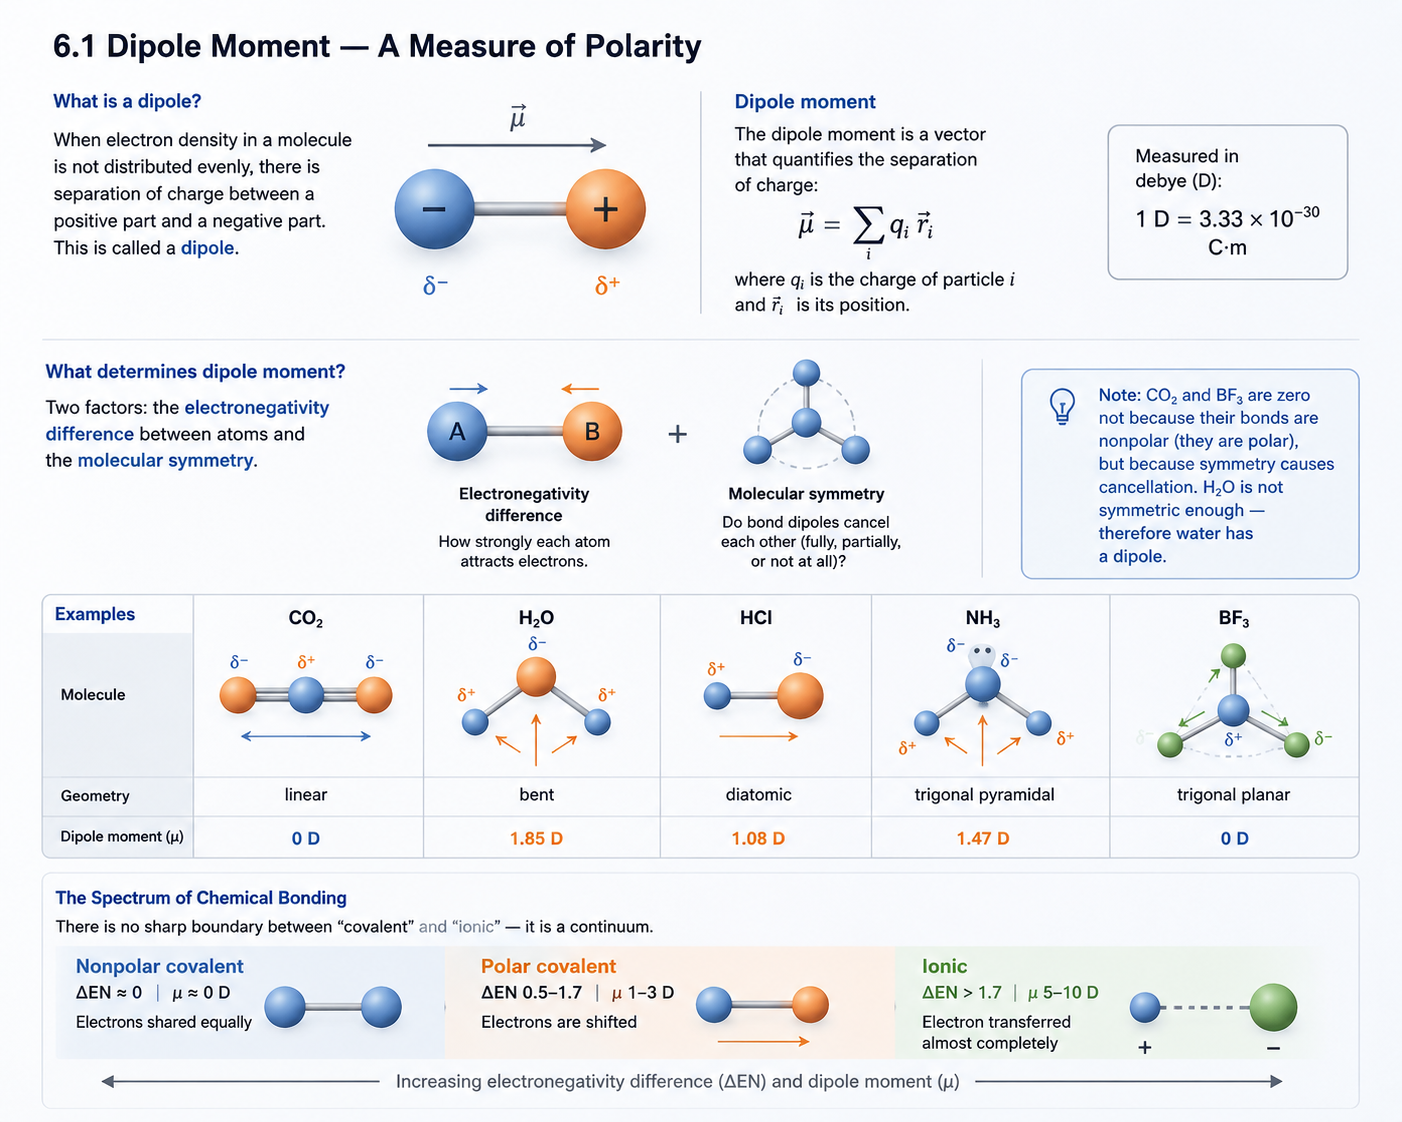
\includegraphics[keepaspectratio]{chapters/../images/image48.dipole.png}}
\#\# 6.2 תיאוריית קשרי הערכיות (VB)

\subsection{הרעיון
הבסיסי}\label{ux5d4ux5e8ux5e2ux5d9ux5d5ux5df-ux5d4ux5d1ux5e1ux5d9ux5e1ux5d9}

תיאוריית VB מבוססת על רעיון אינטואיטיבי: \textbf{שני אלקטרונים
בלתי-מְזוּוָגים מאטומים שונים ``מזדווגים'' ויוצרים קשר}, כאשר הצפיפות
המקסימלית נמצאת בין האטומים.

ארבעה עקרונות:

\begin{enumerate}
\def\labelenumi{\arabic{enumi}.}
\tightlist
\item
  \textbf{כלל האוקטט:} כל אטום שואף ל-8 אלקטרונים בקליפה החיצונית (מימן
  והליום --- ל-2).
\item
  כל אלקטרון בלתי-מזווג נוטה להיזדווג עם אלקטרון בלתי-מזווג של שכן.
\item
  צפיפות האלקטרונים של הזוג המשותף מקסימלית \textbf{בין} האטומים.
\item
  אם האלקטרושליליות שונה, הצפיפות מוסטת לאטום האלקטרושלילי יותר.
\end{enumerate}

\subsection{קשר σ (סיגמה) --- הקשר
הבסיסי}\label{ux5e7ux5e9ux5e8-ux3c3-ux5e1ux5d9ux5d2ux5deux5d4-ux5d4ux5e7ux5e9ux5e8-ux5d4ux5d1ux5e1ux5d9ux5e1ux5d9}

\textbf{קשר σ} נוצר כאשר שני אורביטלים חופפים \textbf{ישירות על הקו
הבין-מרכזי}. החפיפה חזקה.

\begin{itemize}
\tightlist
\item
  \(\sigma_{ss}\): שני אורביטלי \(s\) חופפים (ב-\(\text{H}_2\))
\item
  \(\sigma_{sp}\): אורביטל \(s\) עם אורביטל \(p\) (ב-\(\text{HF}\),
  \(\text{HCl}\))
\item
  \(\sigma_{pp}\): שני אורביטלי \(p\) קצה-מול-קצה
\end{itemize}

\textbf{כלל יסוד:} \textbf{כל קשר יחיד הוא קשר σ בלבד.}

\subsection{קשר π (פאי) --- קשר
נוסף}\label{ux5e7ux5e9ux5e8-ux3c0-ux5e4ux5d0ux5d9-ux5e7ux5e9ux5e8-ux5e0ux5d5ux5e1ux5e3}

\textbf{קשר π} נוצר כאשר אורביטלי \(p\) חופפים \textbf{צִדִּית} --- ממעל
ומתחת לקו הבין-מרכזי. החפיפה חלשה יותר מ-σ.

\begin{itemize}
\tightlist
\item
  קשר כפול = σ \textbf{ועוד} π אחד
\item
  קשר משולש = σ \textbf{ועוד} שני π
\end{itemize}

\textbf{למה π חלש יותר?} כי החפיפה הצידית קטנה יותר מהחפיפה הישירה. לכן
קשר כפול \((σ+π)\) חזק יותר מקשר יחיד \((σ)\), אבל \textbf{לא פי שניים}
--- האנרגיה הנוספת של π קטנה מזו של σ. ןלכן קשר π ניתק יותר בקלות
בתגובות חיבור של, למשל, אלקאנים.

\textbf{דוגמה:} באתאן \(\text{C}_2\text{H}_6\) יש קשר
\(\text{C}-\text{C}\) יחיד (σ בלבד). באתילן (אתן)
\(\text{C}_2\text{H}_4\) יש קשר \(\text{C}=\text{C}\) כפול (σ + π).
האטומים אינם יכולים להסתובב חופשית סביב קשר π --- לכן אצל איזומרי
cis/trans של אלקן, האיזומרים יציבים ונפרדים.
\pandocbounded{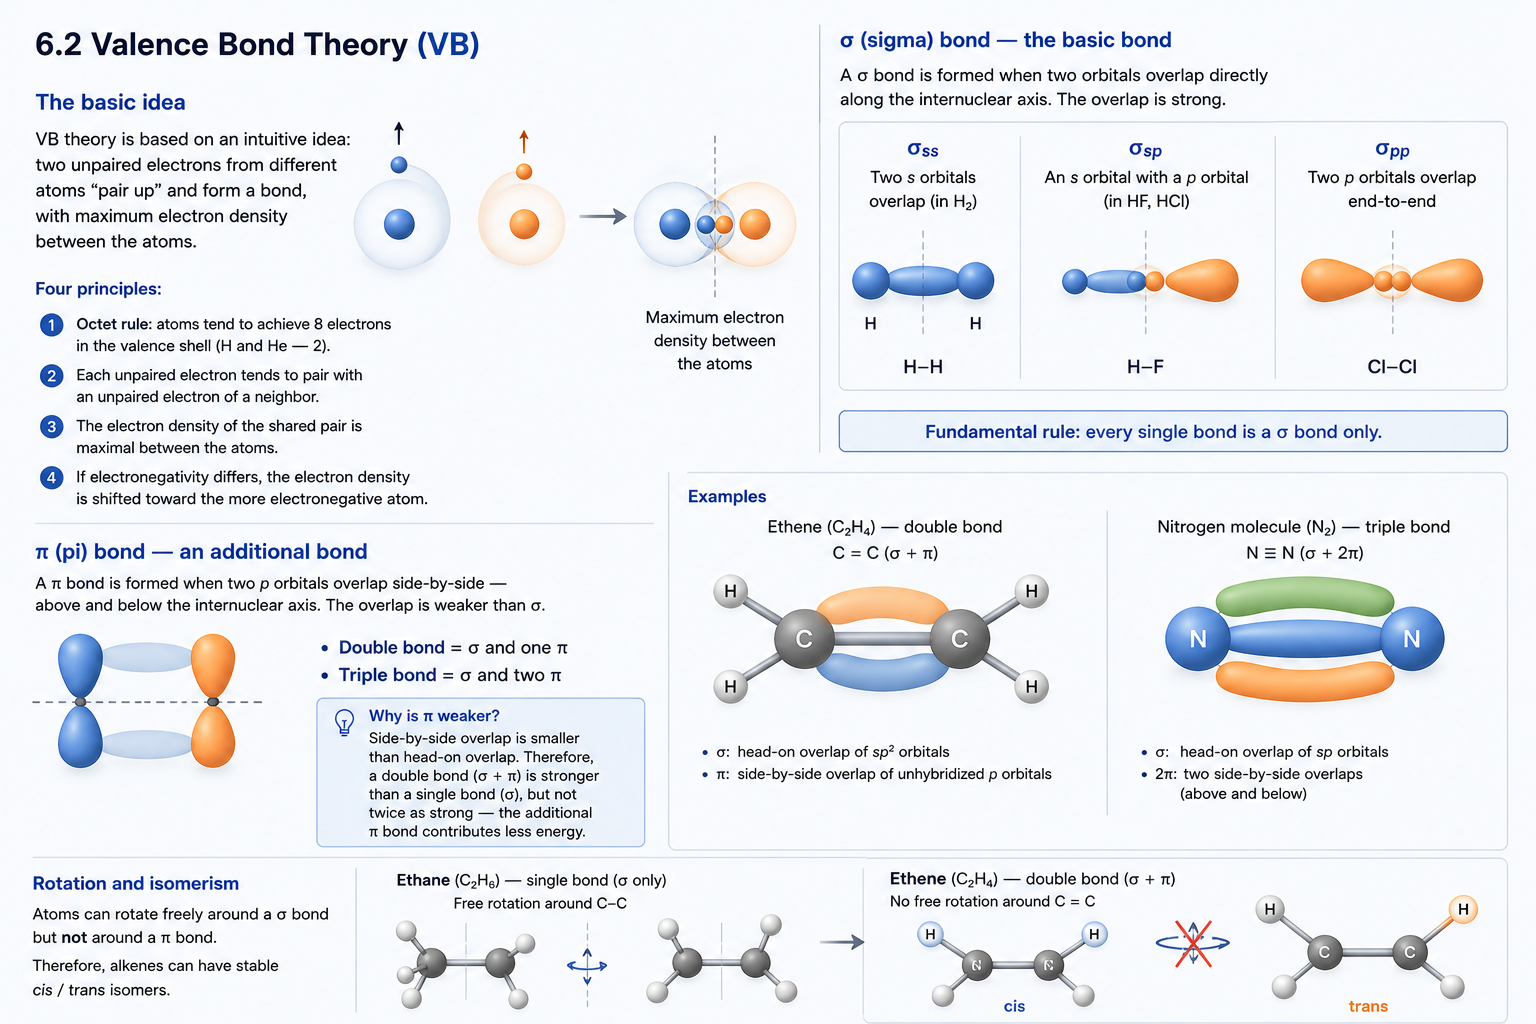
\includegraphics[keepaspectratio]{chapters/../images/image49.ValenceBonds.png}}
\#\# 6.3 היברידיזציה --- מדוע הגיאומטריה אינה מה שמצפים?

\subsection{הבעיה}\label{ux5d4ux5d1ux5e2ux5d9ux5d4-1}

פחמן (\(\text{C}\)) הוא \([He]2s^22p^2\). לפי כלל הזיווג הפשוט, יש לו
שני אלקטרונים בלתי-מזווגים (ב-\(2p\)), לפי כך הערכיות אמורה להיות 2. אבל
פחמן יוצר \textbf{ארבעה} קשרים ב-\(\text{CH}_4\), עם זוויות של
\(109.5°\) --- לא \(90°\) כצפוי עבור אורביטלי \(p\).

\textbf{מדוע?} תיאוריית ה-VB הפשוטה לא יכולה להסביר זאת. כאן נכנסת
\textbf{היברידיזציה}.

\subsection{מה זו
היברידיזציה?}\label{ux5deux5d4-ux5d6ux5d5-ux5d4ux5d9ux5d1ux5e8ux5d9ux5d3ux5d9ux5d6ux5e6ux5d9ux5d4}

\textbf{היברידיזציה} היא תהליך מתמטי שבו אורביטלים אטומיים ``מתמזגים''
ליצירת \textbf{אורביטלים היברידיים} חדשים --- שווים זה לזה בצורה
ובאנרגיה, מכוונים בזוויות שוות כך שהריחוק בין האוריטלים יהיה מקסימלי.

\textbf{שימו לב:} היברידיזציה היא \textbf{מודל מתמטי} --- כלי שעוזר לנו
לחשב ולהבין. האטומים אינם ``מחליטים'' להתהברד. פתרון משוואת שרדינגר מספק
את הקירוב הטוב ביותר למציאות, אך מהווה קושי מיכר בחישוב. היברידיזציה היא
קירוב נוח המאפשר חישוב יותר קל.

\subsection{\texorpdfstring{\(sp^3\) --- מתאן: ארבעה קשרים
שווים}{sp\^{}3 --- מתאן: ארבעה קשרים שווים}}\label{sp3-ux5deux5eaux5d0ux5df-ux5d0ux5e8ux5d1ux5e2ux5d4-ux5e7ux5e9ux5e8ux5d9ux5dd-ux5e9ux5d5ux5d5ux5d9ux5dd}

\textbf{ב-\(\text{CH}_4\)} אורביטל \(2s\) ושלושת אורביטלי \(2p\) של פחמן
מתמזגים לארבעה אורביטלי \(sp^3\) שווים, מכוונים לפינות
\textbf{טטרהדרון}. הזווית: \(109.5°\).

להיברידיזציה מקדים תהליך העירור: אלקטרון אחד ``עולה'' מ-\(2s\) ל-\(2p\)
הריק (העלות: אנרגיית עירור). אחר כך ארבעת האורביטלים מתמזגים. הרווח:
ארבעה קשרים במקום שניים --- ה\textbf{רווח האנרגטי} גדול מה\textbf{עלות}.

\subsection{\texorpdfstring{\(sp^2\) --- שלושה
קשרים}{sp\^{}2 --- שלושה קשרים}}\label{sp2-ux5e9ux5dcux5d5ux5e9ux5d4-ux5e7ux5e9ux5e8ux5d9ux5dd}

\textbf{ב-\(\text{BF}_3\):} אורביטל \(2s\) ושני אורביטלי \(2p\) של אטום
ברום מתמזגים לשלושה אורביטלי \(sp^2\) שווים, מכוונים \textbf{במישור}
בזוויות \(120°\). האורביטל \(2p\) נוסף אינו מאוכלס ואינו פעיל כלל.

\subsection{\texorpdfstring{\(sp^2\) --- שלושה קשרים ועוד π
אחד}{sp\^{}2 --- שלושה קשרים ועוד π אחד}}\label{sp2-ux5e9ux5dcux5d5ux5e9ux5d4-ux5e7ux5e9ux5e8ux5d9ux5dd-ux5d5ux5e2ux5d5ux5d3-ux3c0-ux5d0ux5d7ux5d3}

\textbf{באתן \(C_2H_2\):} קשר π דורש חפיפה צדדית של אורביטלי p טהורים,
הניצבים למישור המולקולה. לכן אורביטל אחד שמור לקשר π ואינו יכול להשתתף
בהיברידיזציה. מה שנותר --- אורביטל s ושני אורביטלי p --- מתמזגים לשלושה
אורביטלי \(sp^2\) שווים, מכוונים במישור בזוויות \(120°\).

\textbf{בבנזן \(C_6H_6\):} שישה פחמנים, כל אחד \(sp^2\), יוצרים שישה
אורביטלי \(p\) הניצבים לטבעת --- הם מתאחדים ל\textbf{מערכת \(\pi\)
מצומדת} שמפוזרת על כל הטבעת (דה-לוקליזציה).

\subsection{\texorpdfstring{\(sp\) --- שני קשרים וגיאומטריה
לינארית}{sp --- שני קשרים וגיאומטריה לינארית}}\label{sp-ux5e9ux5e0ux5d9-ux5e7ux5e9ux5e8ux5d9ux5dd-ux5d5ux5d2ux5d9ux5d0ux5d5ux5deux5d8ux5e8ux5d9ux5d4-ux5dcux5d9ux5e0ux5d0ux5e8ux5d9ux5ea}

\textbf{ב-\(\text{CO}_2\) ובאציטילן (\({HC}\equiv {CH}\)):} אורביטל
\(s\) ואחד מאורביטלי \(p\) מתמזגים ל-\(sp\), זווית \(180°\). שני
אורביטלי \(p\) הנותרים יוצרים שני קשרי π.

\subsection{סיכום
היברידיזציות}\label{ux5e1ux5d9ux5dbux5d5ux5dd-ux5d4ux5d9ux5d1ux5e8ux5d9ux5d3ux5d9ux5d6ux5e6ux5d9ux5d5ux5ea}

{\def\LTcaptype{none} % do not increment counter
\begin{longtable}[]{@{}
  >{\raggedright\arraybackslash}p{(\linewidth - 8\tabcolsep) * \real{0.1068}}
  >{\raggedright\arraybackslash}p{(\linewidth - 8\tabcolsep) * \real{0.1165}}
  >{\raggedright\arraybackslash}p{(\linewidth - 8\tabcolsep) * \real{0.1553}}
  >{\raggedright\arraybackslash}p{(\linewidth - 8\tabcolsep) * \real{0.0971}}
  >{\raggedright\arraybackslash}p{(\linewidth - 8\tabcolsep) * \real{0.5243}}@{}}
\toprule\noalign{}
\begin{minipage}[b]{\linewidth}\raggedright
היברידיזציה
\end{minipage} & \begin{minipage}[b]{\linewidth}\raggedright
מספר קשרים σ
\end{minipage} & \begin{minipage}[b]{\linewidth}\raggedright
גיאומטריה
\end{minipage} & \begin{minipage}[b]{\linewidth}\raggedright
זווית
\end{minipage} & \begin{minipage}[b]{\linewidth}\raggedright
דוגמה
\end{minipage} \\
\midrule\noalign{}
\endhead
\bottomrule\noalign{}
\endlastfoot
\(sp\) & 2 & לינארית & \(180°\) & \(\text{BeCl}_2\), \(\text{CO}_2\),
\(\text{C}_2\text{H}_2\) \\
\(sp^2\) & 3 & משולשת שטוחה & \(120°\) & \(\text{BF}_3\), אתילן, בנזן \\
\(sp^3\) & 4 & טטרהדרלית & \(109.5°\) & \(\text{CH}_4\),
\(\text{NH}_3\), \(\text{H}_2\text{O}\) \\
\(sp^3d\) & 5 & ביפירמידה משולשת & \(90°/120°\) & \(\text{PCl}_5\) \\
\(sp^3d^2\) & 6 & אוקטהדרלית & \(90°\) & \(\text{SF}_6\) \\
\end{longtable}
}

\subsection{זוגות בודדים משנים
זוויות}\label{ux5d6ux5d5ux5d2ux5d5ux5ea-ux5d1ux5d5ux5d3ux5d3ux5d9ux5dd-ux5deux5e9ux5e0ux5d9ux5dd-ux5d6ux5d5ux5d5ux5d9ux5d5ux5ea}

ב-\(\text{NH}_3\): ארבעה זוגות אלקטרונים (שלושה קשרים + זוג בודד).
הגיאומטריה \textbf{אלקטרונית} --- טטרהדרלית. הגיאומטריה
\textbf{מולקולרית} (מה שרואים) --- פירמידה שוות שוקיים. הזוג הבודד לוחץ
חזק יותר מקשר, לכן זווית H-N-H \textbf{קטנה} מ-\(109.5°\) (\(107°\)
בפועל).

ב-\(\text{H}_2\text{O}\): שני קשרים + שני זוגות בודדים. גיאומטריה
זוויתית, \(104.5°\).

\textbf{כלל VSEPR:} זוגות אלקטרונים (קשורים ובודדים) דוחים זה את זה.
ס\textbf{וג} הדחייה: זוג בודד \textgreater{} קשר כפול \textgreater{} קשר
יחיד.
\pandocbounded{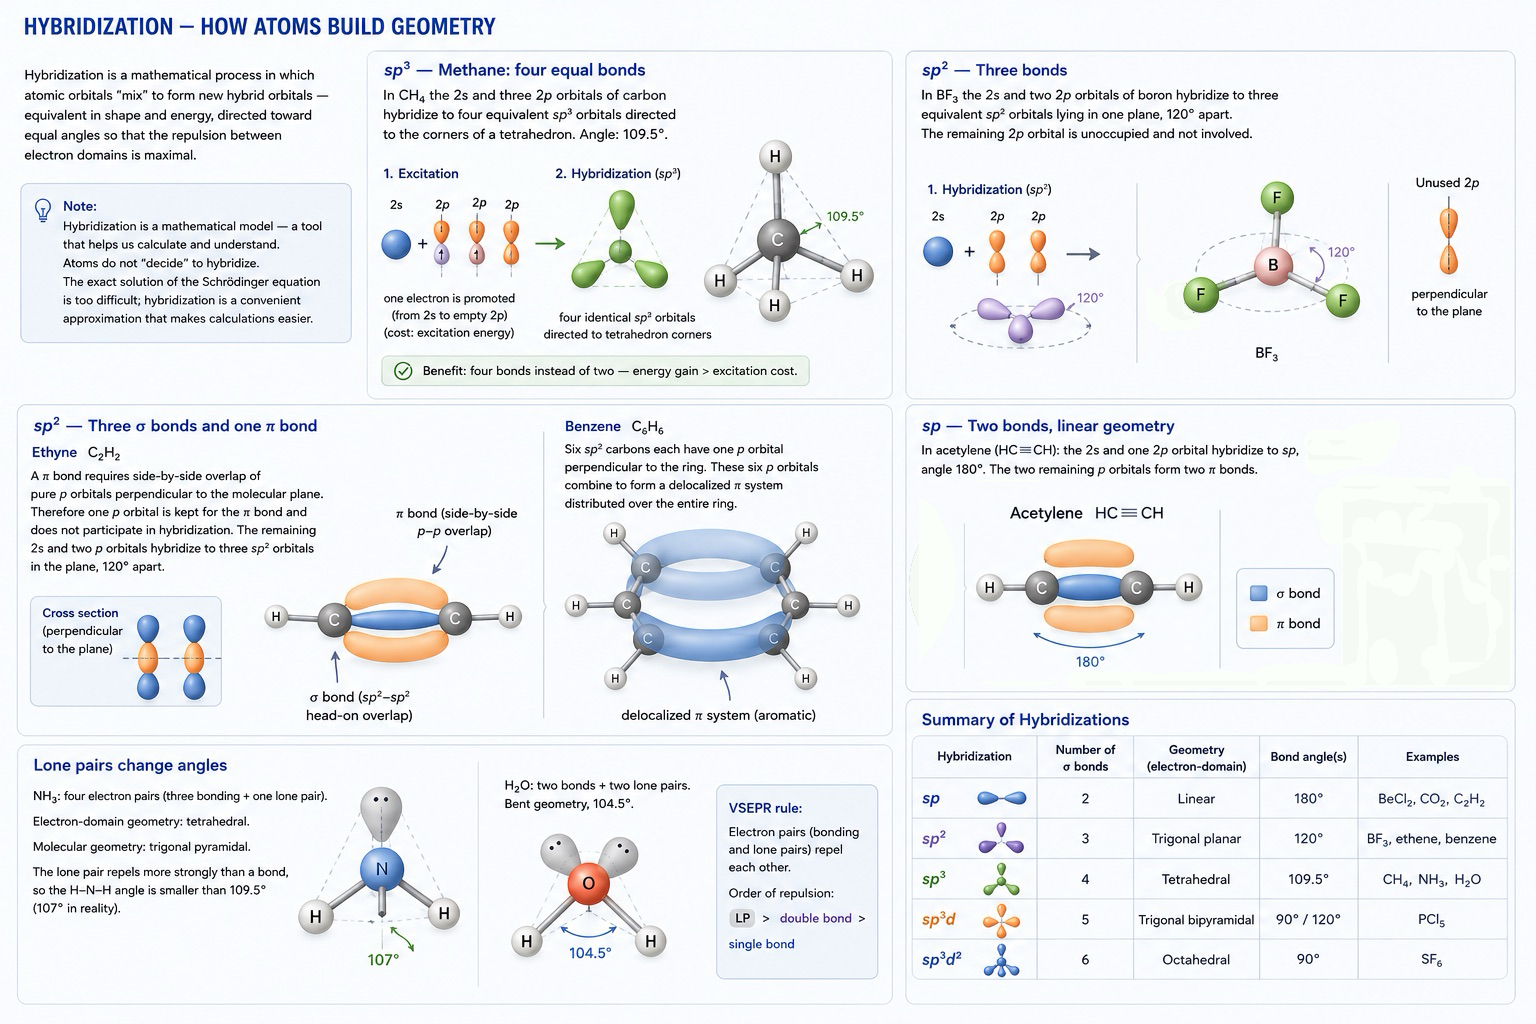
\includegraphics[keepaspectratio]{chapters/../images/image50.Hybridization.png}}
\#\# 6.4 אורביטלים מולקולריים (MO) --- תמונה שלמה יותר

\subsection{מדוע VB לא
מספיקה?}\label{ux5deux5d3ux5d5ux5e2-vb-ux5dcux5d0-ux5deux5e1ux5e4ux5d9ux5e7ux5d4}

התאיורייה של קשרי הערכיות VB) עובדת טוב לרוב המולקולות, אבל נכשלת במקרים
חשובים:

\textbf{במולרולה של חמצן }\(\text{O}_2\) נצפית התנהגות פרמכנטית** וזה
בניגוד ל-VB המנבאת שלכל האלקטרונים ב-\(\text{O}_2\) יש זוגות (וזה מתאים
להתנהגות הדיאמגנטית). תיאוריית MO מסבירה זאת בהצלחה.

\textbf{בנזן:} VB דורשת שני מבנים רזוננסיים (Kekulé). MO נותנת תמונה
ישירה של הדה-לוקליזציה.

\textbf{ספקטרוסקופיה:} MO מסבירה אילו מעברים אפשריים ואילו אסורים.

\subsection{הרעיון המרכזי של
MO}\label{ux5d4ux5e8ux5e2ux5d9ux5d5ux5df-ux5d4ux5deux5e8ux5dbux5d6ux5d9-ux5e9ux5dc-mo}

\textbf{אורביטלים אטומיים מתחברים לאורביטלים מולקולריים השייכים לכל
המולקולה}. מ-\(N\) אורביטלים אטומיים מתקבלים \(N\) אורביטלים מולקולריים:
\textbf{חצי מהם קושרים} (אנרגיה נמוכה מהאורביטל האטומי) ו\textbf{החצי
השני מהם אנטי-קושרים} (אנרגיה גבוהה יותר).

\textbf{אורביטל קושר} --- נוצר מחפיפת אורביטלים \textbf{באותה פאזה}
(\(+\) עם \(+\)). צפיפות האלקטרונים גדלה \textbf{בין} האטומים.

\textbf{אורביטל אנטי-קושר} --- נוצר מחפיפת אורביטלים \textbf{בפאזות
הפוכות} (\(+\) עם \(-\)). בשל כך נוצר \textbf{מישור אפס} (node) בין
האטומים שבו צפיפות האלקטרון אפסית. אורביטל כזה איננו מקשר אטומים אלא
מחליש קשר ביניהם. אורביטלים אנטי-קושרים מסומנים בכוכבית *.

\subsection{סדר הקשר}\label{ux5e1ux5d3ux5e8-ux5d4ux5e7ux5e9ux5e8}

\[\text{bond order} = \frac{N_\text{bonding} - N_\text{anti-bonding}}{2}\]

\begin{itemize}
\tightlist
\item
  סדר קשר 1 = קשר יחיד
\item
  סדר קשר 2 = קשר כפול
\item
  סדר קשר 0 = אין קשר (המולקולה אינה יציבה)
\item
  סדר קשר שבור = יש אלקטרונים בלתי-מזווגים → פרמגנטי
\end{itemize}

\subsection{\texorpdfstring{דוגמה:
\(\text{O}_2\)}{דוגמה: \textbackslash text\{O\}\_2}}\label{ux5d3ux5d5ux5d2ux5deux5d4-texto_2}

קונפיגורציית MO (מהאנרגיה הנמוכה כלפי מעלה, רק אורביטלי ערכיות):

\[(\sigma_{2s})^2(\sigma_{2s}^*)^2(\sigma_{2p})^2(\pi_{2p})^4(\pi_{2p}^*)^2\]

\textbf{סדר הקשר:} \[\frac{(2+2+4) - (2+2)}{2} = \frac{8-4}{2} = 2\]

קשר כפול (\(\text{O}=\text{O}\)) --- נכון!

\textbf{פרמגנטיות:} שני אלקטרוני \((\pi_{2p}^*)^2\) --- לפי כלל הונד, הם
בשני אורביטלי \(\pi^*\) שונים עם ספינים מקבילים → שני אלקטרונים
בלתי-מזורגים → \textbf{פרמגנטי}. VB לא יכלה לנבא זאת.

\subsection{HOMO ו-LUMO}\label{homo-ux5d5-lumo}

\textbf{HOMO} (Highest Occupied Molecular Orbital) --- האורביטל
המולקולרי המלא בעל האנרגיה הגבוהה ביותר.

\textbf{LUMO} (Lowest Unoccupied Molecular Orbital) --- האורביטל
המולקולרי הריק בעל האנרגיה הנמוכה ביותר.

\textbf{למה חשוב?} כמעט כל המעברים האלקטרוניים הראשונים הם HOMO → LUMO.
הם קובעים:

\begin{itemize}
\tightlist
\item
  את הצבע של המולקולה (האנרגיה של הפוטון הנספג)
\item
  את הריאקטיביות הכימית
\item
  את תכונות הקוואנטים האלקטרוניים
  \pandocbounded{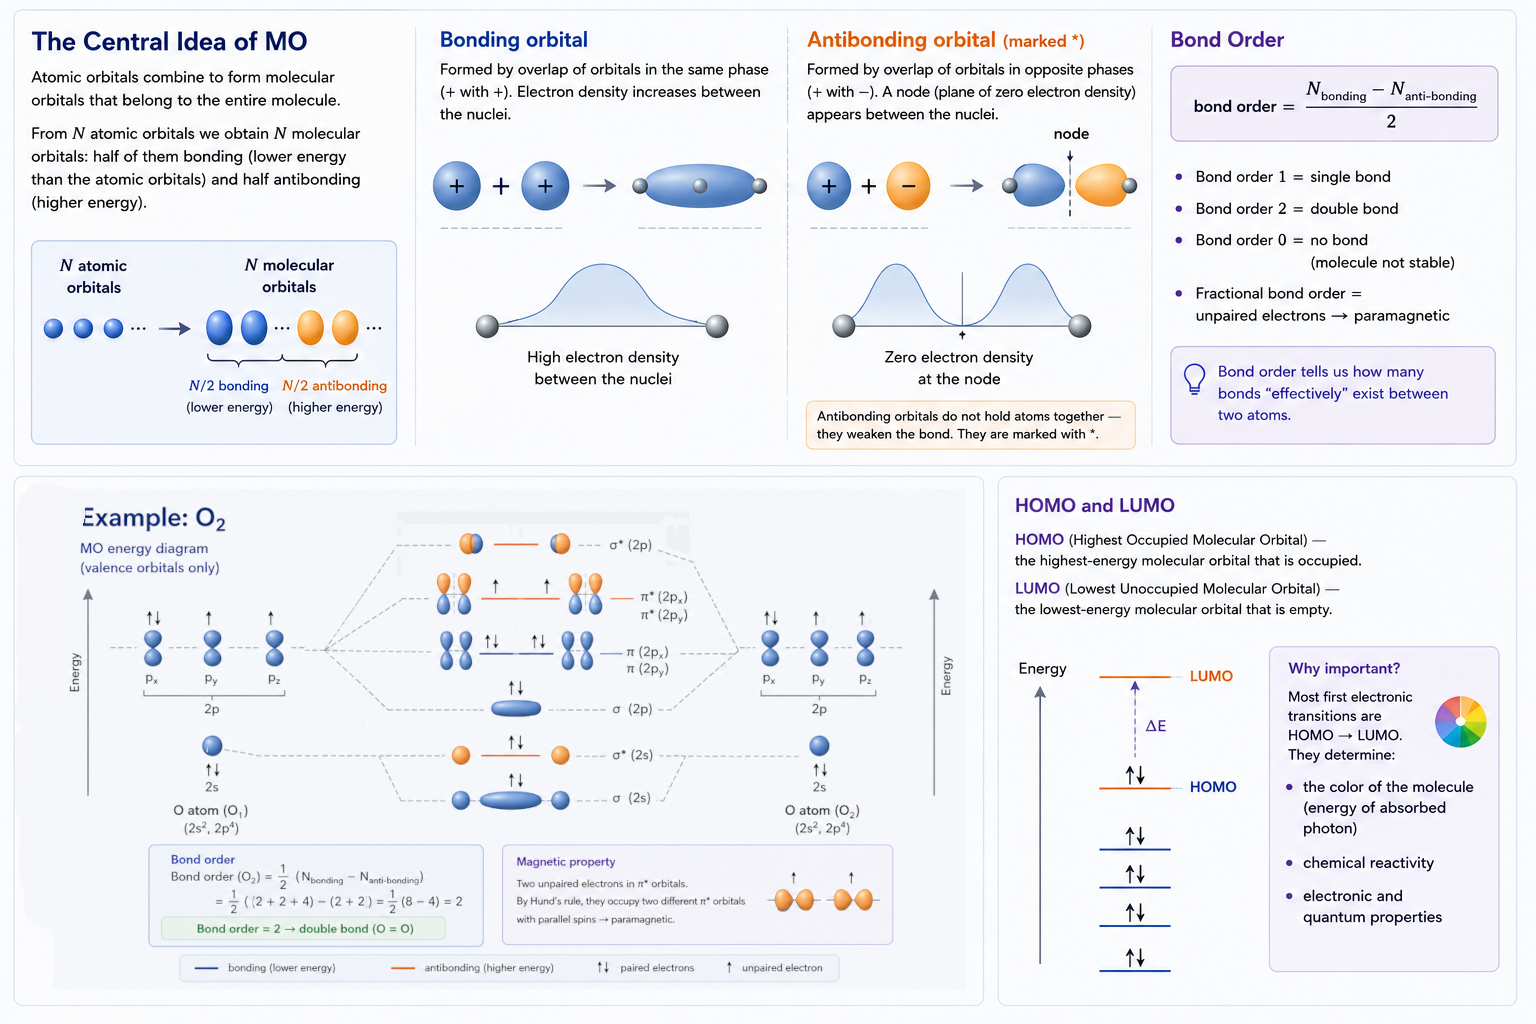
\includegraphics[keepaspectratio]{chapters/../images/image51.MO.png}}
  \#\# 6.5 ספקטרוסקופיה מולקולרית --- שלוש שכבות אנרגיה
\end{itemize}

\subsection{קירוב
בורן-אופנהיימר}\label{ux5e7ux5d9ux5e8ux5d5ux5d1-ux5d1ux5d5ux5e8ux5df-ux5d0ux5d5ux5e4ux5e0ux5d4ux5d9ux5d9ux5deux5e8}

הגרעינים כבדים בהרבה מהאלקטרונים. לכן הם זזים לאט יותר בסדרי גודל.
\textbf{קירוב בורן-אופנהיימר} מניח שאפשר לפצל:

\[E_\text{total} = E_\text{electron} + E_\text{vibration} + E_\text{rotation}\]

שלוש תרומות, שלוש סקאלות אנרגיה, שלושה אזורי ספקטרום:

{\def\LTcaptype{none} % do not increment counter
\begin{longtable}[]{@{}
  >{\raggedright\arraybackslash}p{(\linewidth - 8\tabcolsep) * \real{0.0952}}
  >{\raggedright\arraybackslash}p{(\linewidth - 8\tabcolsep) * \real{0.3095}}
  >{\raggedright\arraybackslash}p{(\linewidth - 8\tabcolsep) * \real{0.0833}}
  >{\raggedright\arraybackslash}p{(\linewidth - 8\tabcolsep) * \real{0.3690}}
  >{\raggedright\arraybackslash}p{(\linewidth - 8\tabcolsep) * \real{0.1429}}@{}}
\toprule\noalign{}
\begin{minipage}[b]{\linewidth}\raggedright
סוג מעבר
\end{minipage} & \begin{minipage}[b]{\linewidth}\raggedright
מנגנון
\end{minipage} & \begin{minipage}[b]{\linewidth}\raggedright
אנרגיה
\end{minipage} & \begin{minipage}[b]{\linewidth}\raggedright
אורך גל
\end{minipage} & \begin{minipage}[b]{\linewidth}\raggedright
ספקטרוסקופיה
\end{minipage} \\
\midrule\noalign{}
\endhead
\bottomrule\noalign{}
\endlastfoot
אלקטרוני & אלקטרון עובר בין אורביטלים & גבוהה & UV--נראה
(\(200\)--\(800;\text{nm}\)) & UV-Vis \\
תנודתי & קשרים מתארכים/מתקצרים & בינונית & IR
(\(2.5\)--\(25;\mu\text{m}\)) & IR \\
סיבובי & המולקולה מסתובבת & נמוכה & מיקרוגל--IR-רחוק & Microwave \\
\end{longtable}
}

\subsection{מה גורם
לספקטרום?}\label{ux5deux5d4-ux5d2ux5d5ux5e8ux5dd-ux5dcux5e1ux5e4ux5e7ux5d8ux5e8ux5d5ux5dd}

\textbf{עיקרון יסוד:} מולקולה בולעת/פולטת פוטון כאשר \textbf{מומנט
הדיפול שלה משתנה} במהלך הפעולה (תנועה או מעבר).

\begin{itemize}
\tightlist
\item
  \textbf{מעבר אלקטרוני:} הצפיפות האלקטרונית עוברת ממקום למקום → מומנט
  דיפול משתנה → ספקטרום UV-Vis
\item
  \textbf{תנודה פעילה ב-IR:} הקשרים זוזים → מומנט דיפול משתנה → ספקטרום
  IR
\item
  \textbf{סיבוב פעיל:} המולקולה מסתובבת → כיוון הדיפול משתנה → ספקטרום
  מיקרוגל
\end{itemize}

\textbf{מסקנה:} \(\text{N}_2\), \(\text{O}_2\), \(\text{H}_2\) --- ללא
מומנט דיפול, ללא תנודות פעילות ב-IR. ל-\(\text{CO}_2\) יש מומנט דיפול
אפסי --- אבל \textbf{תנודות אסימטריות} משנות את הדיפול ולכן פעילות ב-IR.
לכן \(\text{CO}_2\) הוא גז חממה חשוב. \#\# 6.6 ספקטרוסקופיה IR --- כלי
זיהוי מבני

\subsection{מהן תנודות
מולקולריות?}\label{ux5deux5d4ux5df-ux5eaux5e0ux5d5ux5d3ux5d5ux5ea-ux5deux5d5ux5dcux5e7ux5d5ux5dcux5e8ux5d9ux5d5ux5ea}

מולקולה עם \(N\) אטומים יכולה לנוע ב-\(3N\) דרכים עצמאיות. שלוש מהן הן
תנועת הקבוצה כולה (טרנסלציה), שלוש --- סיבוב הקבוצה (לינארי: שניים).
הנותרים הם \textbf{תנודות פנימיות}:

\begin{itemize}
\tightlist
\item
  מולקולה לא-לינארית: \(3N - 6\) תנודות
\item
  מולקולה לינארית: \(3N - 5\) תנודות
\end{itemize}

\textbf{\(\text{H}_2\text{O}\)} (\(N=3\), לא-לינארית): \(3\cdot3-6 = 3\)
תנודות.

\textbf{\(\text{CO}_2\)} (\(N=3\), לינארית): \(3\cdot3-5 = 4\) תנודות.

\subsection{שלושת תנודות
המים}\label{ux5e9ux5dcux5d5ux5e9ux5ea-ux5eaux5e0ux5d5ux5d3ux5d5ux5ea-ux5d4ux5deux5d9ux5dd}

\textbf{1. מתיחה סימטרית} (symmetric stretching): שני קשרי O--H מתארכים
ומתקצרים \textbf{בו-זמנית ובאותה כמות}. המולקולה שומרת על סימטריה →
שינוי \(\mu\) קטן → פעילה ב-IR, אך חלשה.

\textbf{2. מתיחה אסימטרית} (asymmetric stretching): קשר אחד מתארך כשהשני
מתקצר → הסימטריה נשברת → שינוי \(\mu\) גדול → \textbf{פעילה מאוד ב-IR}.

\textbf{3. כיפוף} (bending): זווית H--O--H משתנה → שינוי \(\mu\) → פעילה
ב-IR.

\subsection{``טביעת אצבע''
ספקטרלית}\label{ux5d8ux5d1ux5d9ux5e2ux5ea-ux5d0ux5e6ux5d1ux5e2-ux5e1ux5e4ux5e7ux5d8ux5e8ux5dcux5d9ux5ea}

כל קבוצה פונקציונלית סופגת בתדירות \textbf{אופיינית} שאינה משתנה הרבה
ממולקולה למולקולה:

{\def\LTcaptype{none} % do not increment counter
\begin{longtable}[]{@{}ll@{}}
\toprule\noalign{}
קבוצה & תדירות ספיגה \\
\midrule\noalign{}
\endhead
\bottomrule\noalign{}
\endlastfoot
O--H (אלכוהול) & \(3200\)--\(3600;\text{cm}^{-1}\) (רחב) \\
N--H & \(3300\)--\(3500;\text{cm}^{-1}\) \\
C--H & \(2850\)--\(3000;\text{cm}^{-1}\) \\
C≡N & \(2200\)--\(2260;\text{cm}^{-1}\) \\
C=O (קרבוניל) & \(1700\)--\(1750;\text{cm}^{-1}\) \\
C=C & \(1620\)--\(1680;\text{cm}^{-1}\) \\
C--O & \(1000\)--\(1300;\text{cm}^{-1}\) \\
\end{longtable}
}

ספקטרום IR של חומר לא-מוכר הוא ``טביעת אצבע'' כימית: ניתן לזהות אילו
קבוצות פונקציונליות קיימות ואילו לא.

\begin{quote}
\textbf{יישום:} בתעשיית הפולימרים, בספרנות כימית ובאנליזה סביבתית ---
ספקטרוסקופיית IR היא כלי יומיומי לזיהוי חומרים.
\pandocbounded{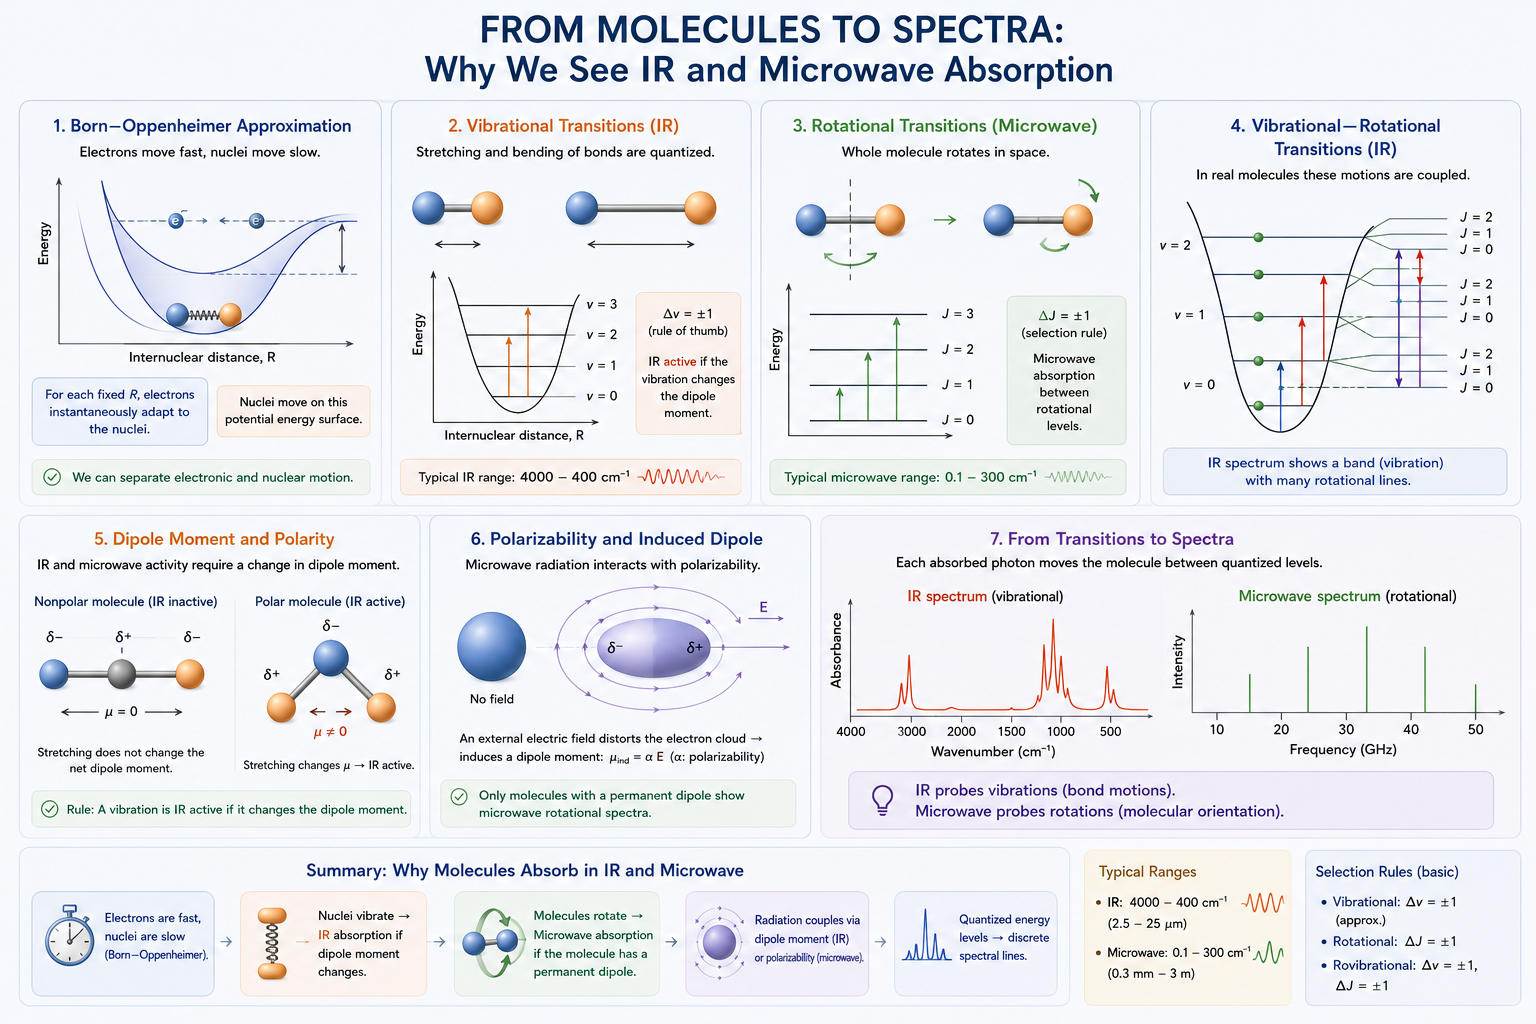
\includegraphics[keepaspectratio]{chapters/../images/image52.MolecularSpectra.png}}
\#\# 6.7 סיכום: VB מול MO --- מתי להשתמש במה?
\end{quote}

{\def\LTcaptype{none} % do not increment counter
\begin{longtable}[]{@{}ll@{}}
\toprule\noalign{}
שאלה & גישה מומלצת \\
\midrule\noalign{}
\endhead
\bottomrule\noalign{}
\endlastfoot
מה הגיאומטריה של המולקולה? & VB + VSEPR \\
מה סדר הקשר? & MO \\
מה הצבע? & MO (HOMO-LUMO gap) \\
האם המולקולה פרמגנטית? & MO \\
אילו קבוצות פונקציונליות יש? & IR \\
האם הקשר קוולנטי או יוני? & מומנט דיפול \\
\end{longtable}
}

שתי התיאוריות \textbf{לא סותרות} --- הן שתי דרכים לקרב את פתרון משוואת
שרדינגר. MO מדויקת יותר; VB אינטואיטיבית יותר. בפועל, כימאים משתמשים
בשתיהן לפי הצורך. \#\# סיכום

שישה נושאים עיקריים בפרק:

\textbf{מומנט דיפול} --- מדד כמותי לפולריות. נקבע על ידי הפרש
אלקטרושליליות \textbf{וסימטריה}. ספקטרום הקשר: קוולנטי ← רצף ← יוני.

\textbf{קשרי σ ו-π} --- σ על הציר הבין-מרכזי, חזק. π צִדִּי, חלש יותר. כל
קשר יחיד = σ; כפול = σ+π; משולש = σ+ππ.

\textbf{היברידיזציה} --- מיזוג אורביטלי \(s\) ו-\(p\) לאורביטלים
היברידיים שווים. מסביר את הגיאומטריה. \(sp^3\)→\(109.5°\);
\(sp^2\)→\(120°\); \(sp\)→\(180°\).

\textbf{אורביטלים מולקולריים} --- אורביטלים השייכים לכל המולקולה. סדר
הקשר = (קושרים−אנטי-קושרים)/2. מסביר פרמגנטיות ועוד.

\textbf{HOMO-LUMO} --- הפרש האנרגיה ביניהם קובע את הצבע ואת הריאקטיביות.

\textbf{ספקטרוסקופיה IR} --- מודדת תנודות שמשנות מומנט דיפול. כל קבוצה
פונקציונלית בתדירות אופיינית. כלי זיהוי יומיומי.

\bookmarksetup{startatroot}

\chapter{פרק 7 --- מצבי צבירה ותכונות
נוזלים}\label{ux5e4ux5e8ux5e7-7-ux5deux5e6ux5d1ux5d9-ux5e6ux5d1ux5d9ux5e8ux5d4-ux5d5ux5eaux5dbux5d5ux5e0ux5d5ux5ea-ux5e0ux5d5ux5d6ux5dcux5d9ux5dd}

\section{מבוא: מה הופך חומר למה
שהוא?}\label{ux5deux5d1ux5d5ux5d0-ux5deux5d4-ux5d4ux5d5ux5e4ux5da-ux5d7ux5d5ux5deux5e8-ux5dcux5deux5d4-ux5e9ux5d4ux5d5ux5d0}

כאשר מים הופכים לקרח, אין שינוי כימי --- אותן מולקולות
\(\text{H}_2\text{O}\), אותו הרכב. מה שמשתנה הוא \textbf{מצב הצבירה} ---
האופן שבו המולקולות מסודרות ומתנהגות ביחס זו לזו. הבנת מצבי הצבירה היא
גשר ישיר בין מה שלמדנו על האטום הבודד לבין תכונות החומר המוצק שנלמד
בפרקים הבאים. \#\# 7.1 תכונות מיקרוסקופיות ומאקרוסקופיות

\subsection{ההבחנה
הבסיסית}\label{ux5d4ux5d4ux5d1ux5d7ux5e0ux5d4-ux5d4ux5d1ux5e1ux5d9ux5e1ux5d9ux5ea}

\textbf{תכונות מיקרוסקופיות} תלויות בחלקיקים בודדים ואינן ניתנות למדידה
ישירה בידינו:

\begin{itemize}
\tightlist
\item
  מסה אטומית/מולקולרית
\item
  מאפיינים ספקטרליים
\item
  גודל וצורת האטום
\end{itemize}

\textbf{תכונות מאקרוסקופיות} תלויות במספר גדול של חלקיקים וניתנות למדידה
ישירה:

\begin{itemize}
\tightlist
\item
  נפח, צפיפות
\item
  טמפרטורה, לחץ
\item
  צבע, מצב צבירה
\end{itemize}

\textbf{דוגמה חשובה:} לאטום בודד אין ``טמפרטורה''. טמפרטורה היא
\textbf{הממוצע הסטטיסטי} של האנרגיה הקינטית של אוסף חלקיקים רבים בתנועה
אקראית. אטום אחד --- אין ממוצע, אין טמפרטורה.

\textbf{פאזה} היא צורה פיזית ייחודית של חומר --- כלומר, מצב שבו לכל
חלקיקי החומר אותה סביבה מיקרוסקופית. \#\# 7.2 כוחות בין-אטומיים
ופוטנציאל לנארד-ג'ונס

\subsection{מדוע אטומים נמשכים זה
לזה?}\label{ux5deux5d3ux5d5ux5e2-ux5d0ux5d8ux5d5ux5deux5d9ux5dd-ux5e0ux5deux5e9ux5dbux5d9ux5dd-ux5d6ux5d4-ux5dcux5d6ux5d4}

בין כל שני אטומים פועלים בו-זמנית שני כוחות מנוגדים:

\textbf{כוח משיכה} --- נובע מ\textbf{כוחות ון-דר-ולס} (van der Waals).
מקורם בתנודות בצפיפות האלקטרונים: בכל רגע נתון, ההתפלגות האלקטרונית אינה
מושלמת ונוצרים \textbf{דיפולים מיידיים} --- שמושכים דיפולים מושרים
בשכנים. כוח זה פרופורציונלי ל-\(r^{-6}\).

שלושה סוגי אינטראקציות ון-דר-ולס:

\begin{itemize}
\tightlist
\item
  \textbf{דיפול-דיפול} (Keesom): בין מולקולות פולריות קבועות
\item
  \textbf{דיפול-דיפול מושרה} (Debye): דיפול קבוע מושרה דיפול בשכן
\item
  \textbf{דיספרסיה} (London): בין כל שני אטומים --- גם ניטרליים לחלוטין.
  זהו הסוג האוניברסלי.
\end{itemize}

\textbf{כוח דחייה} --- נובע מ\textbf{עקרון פאולי}: כאשר אטומים מתקרבים
מאוד, ענני האלקטרונים חופפים ועקרון פאולי אוסר על אותו מצב קוונטי →
דחייה חזקה מאוד, פרופורציונלית ל-\(r^{-12}\).
\pandocbounded{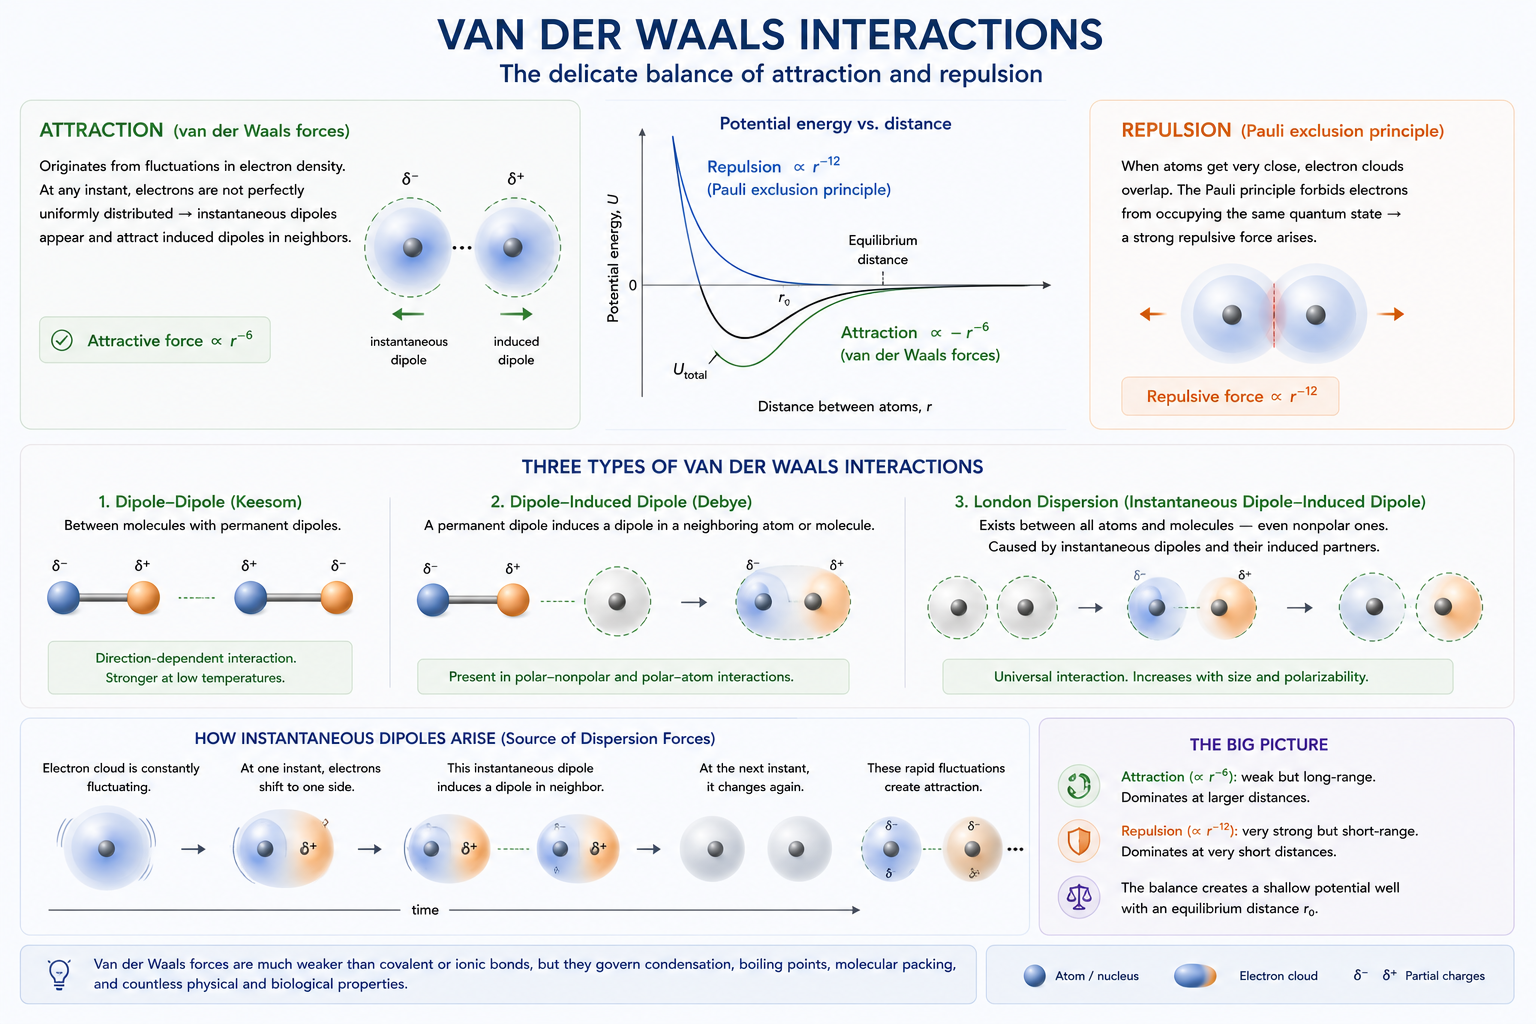
\includegraphics[keepaspectratio]{chapters/../images/image53.VanDerVaals.png}}
\#\#\# פוטנציאל לנארד-ג'ונס

שילוב שני הכוחות נותן את \textbf{פוטנציאל לנארד-ג'ונס} (Lennard-Jones
potential):

\[V(r) = 4\epsilon \left[\left(\frac{\sigma}{r}\right)^{12} - \left(\frac{\sigma}{r}\right)^{6}\right]\]

כאשר:

\begin{itemize}
\tightlist
\item
  \(\epsilon\) --- עומק \textbf{בור הפוטנציאל} (מידת עוצמת המשיכה)
\item
  \(\sigma\) --- המרחק שבו הפוטנציאל אפסי (בערך ``רדיוס'' האטום)
\item
  \(r_0 = 2^{1/6}\sigma\) --- המרחק שבו הפוטנציאל מינימלי (מיקום שיווי
  המשקל)
\end{itemize}

\textbf{קריאת הגרף:}

\begin{itemize}
\tightlist
\item
  ב-\(r < r_0\): דחייה (האטומים קרובים מדי)
\item
  ב-\(r = r_0\): שיווי משקל --- כוחות מאוזנים
\item
  ב-\(r > r_0\): משיכה (האטומים מתקרבים זה לזה)
\item
  ב-\(r \to \infty\): \(V \to 0\) (אין אינטראקציה)
\end{itemize}

\textbf{שתי מסקנות:}

\begin{enumerate}
\def\labelenumi{\arabic{enumi}.}
\tightlist
\item
  כל אטום יציב \textbf{בתוך חומר} יותר מאשר בוואקום --- הוא נמצא בתוך
  בור פוטנציאל
\item
  עומק הבור תלוי בסביבה --- ב-\(\text{Cu}\) שונה מב-\(\text{Fe}\) שונה
  מב-\(\text{NaCl}\)
  \pandocbounded{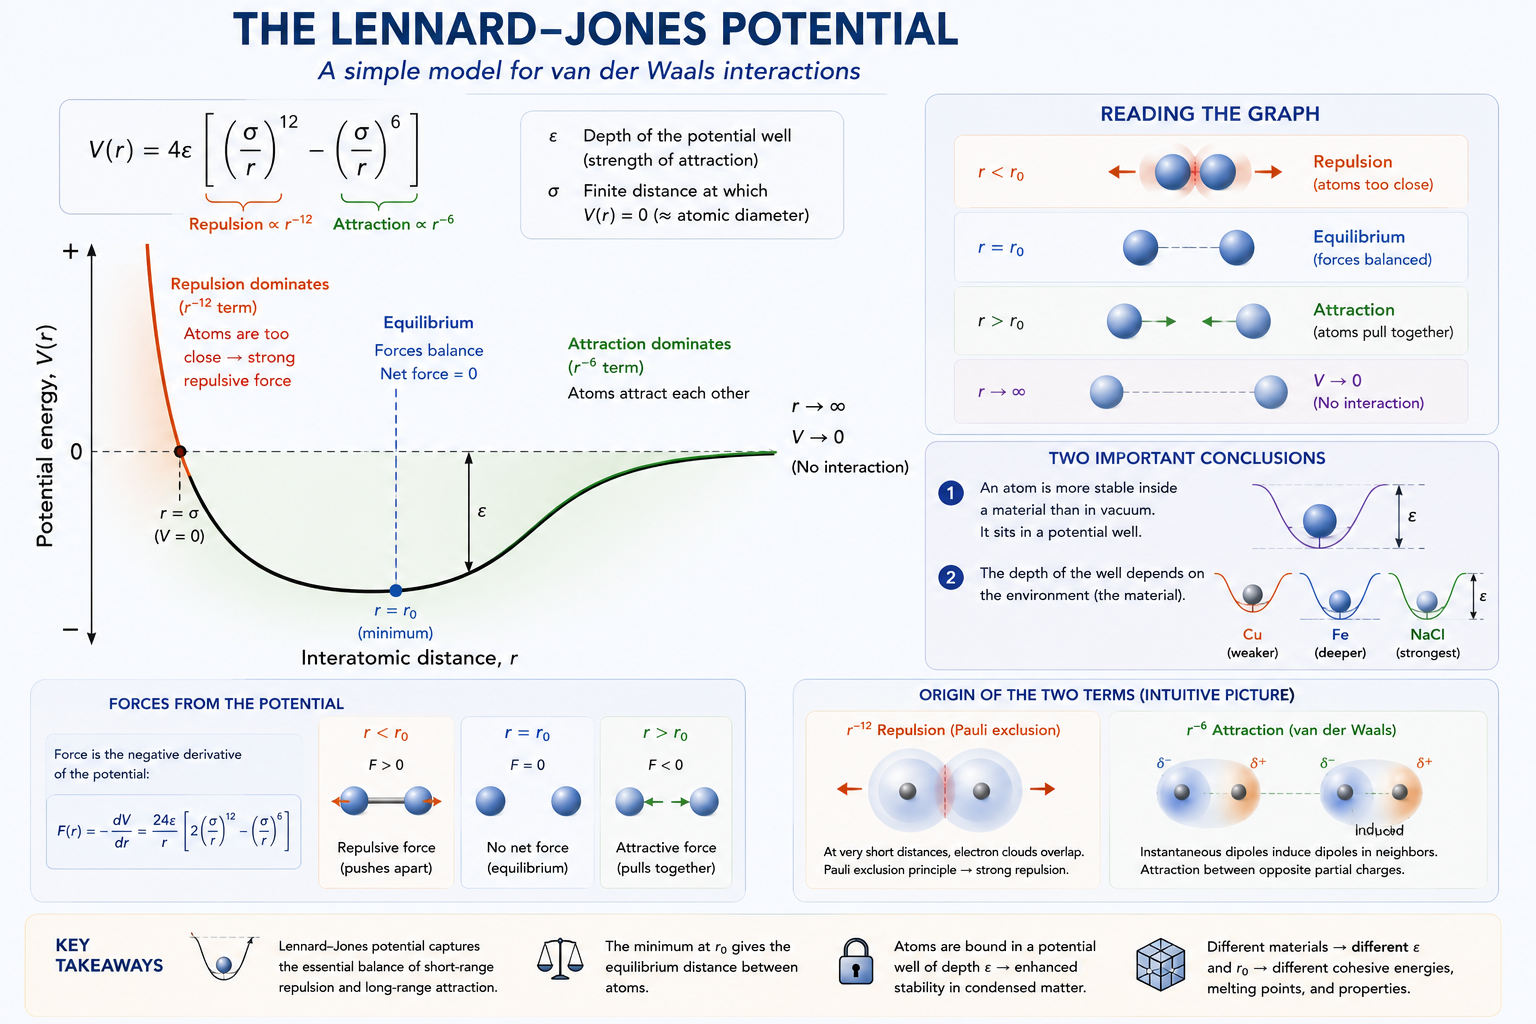
\includegraphics[keepaspectratio]{chapters/../images/image54.LennardJones.png}}
  \#\# 7.3 חלקיק בודד, שטח וגוש --- מהי פאזה?
\end{enumerate}

\subsection{שלושה סוגי
חלקיקים}\label{ux5e9ux5dcux5d5ux5e9ux5d4-ux5e1ux5d5ux5d2ux5d9-ux5d7ux5dcux5e7ux5d9ux5e7ux5d9ux5dd}

בתוך חומר, כל חלקיק שונה מהאחר לפי \textbf{סביבתו}:

\textbf{חלקיק בודד} --- בוואקום, או מוקף לחלוטין בחלקיקי חומר אחר. אין
שכנים מאותו חומר.

\textbf{חלקיק שטחי} --- מוקף בחלקיקי החומר שלו מצד אחד, ובחלל (או חומר
אחר) מהצד השני. יש לו \textbf{שכנים חסרים} --- ולכן הוא נמצא באנרגיה
גבוהה יותר מחלקיק הגוש.

\textbf{חלקיק גוש} (bulk) --- מוקף לחלוטין בחלקיקי החומר שלו. זהו המצב
האנרגטי הנמוך ביותר.

אנרגית חלקיק גוש:

\[E_\text{bulk} = E_\text{vac} - n \cdot E_\text{VdW}\]

כאשר \(n\) הוא מספר השכנים (מספר הקואורדינציה).

אנרגיית חלקיק שטחי:

\[E_\text{surf} = E_\text{vac} - m \cdot E_\text{VdW}, \quad m \approx \frac{n}{2} < n\]

לכן: \(E_\text{bulk} < E_\text{surf} < E_\text{vac}\)

\pandocbounded{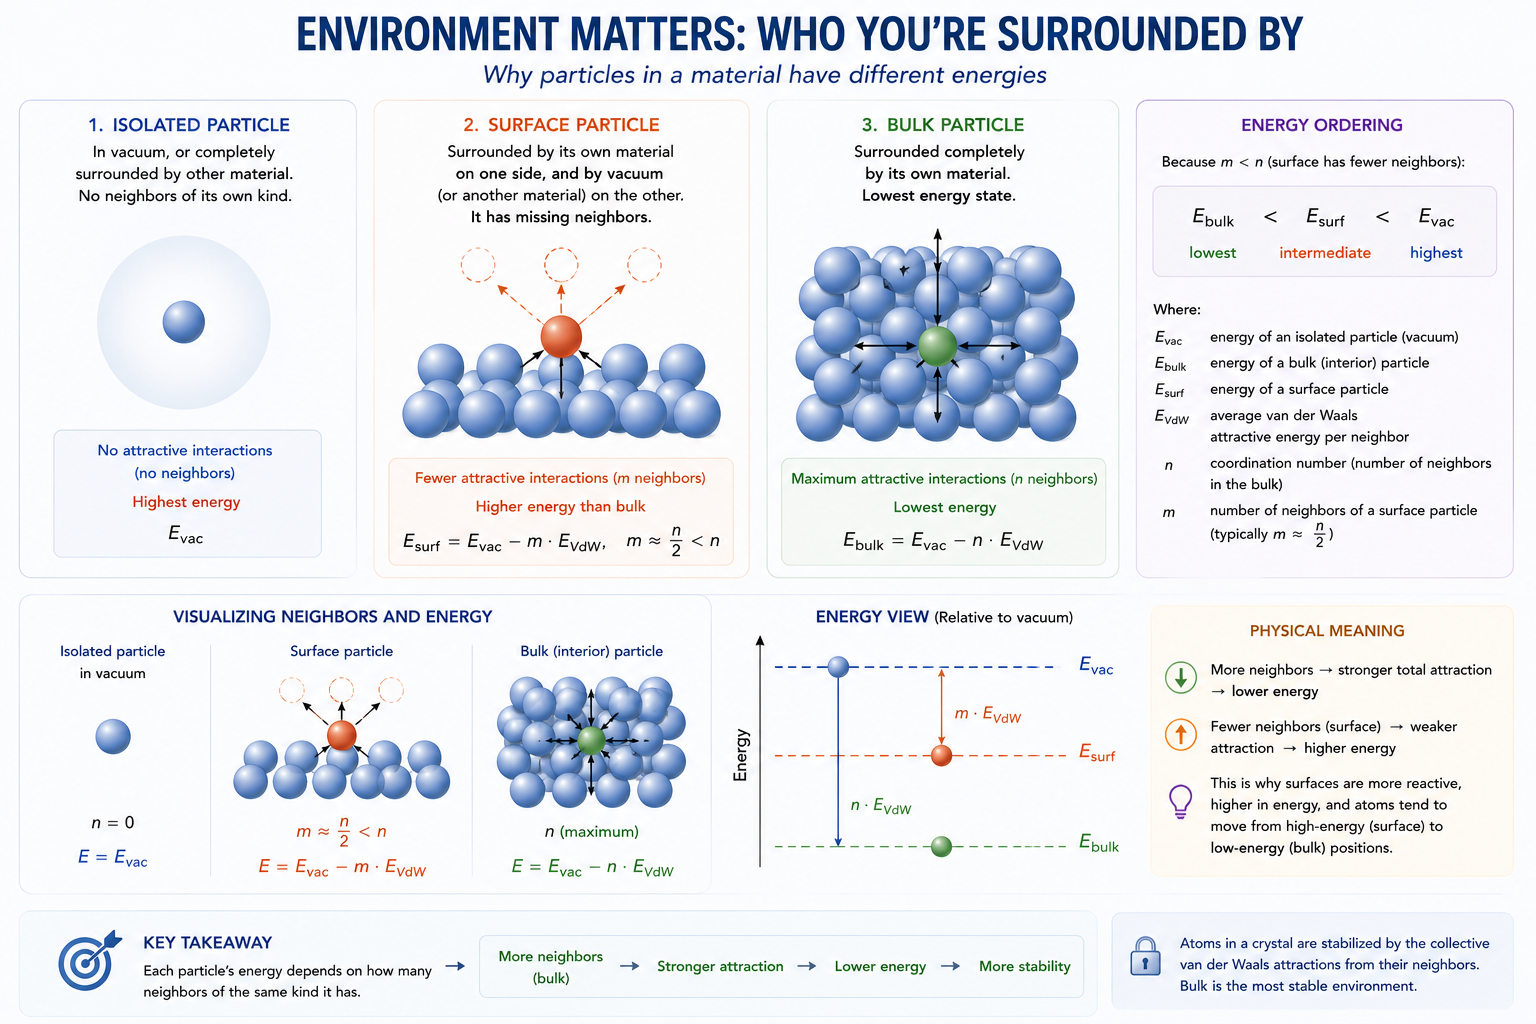
\includegraphics[keepaspectratio]{chapters/../images/image55.ParticlesPhases.png}}
\#\#\# מתי קיימת פאזה?

\textbf{פאזה} קיימת כאשר מספר חלקיקי הגוש גדול \textbf{בהרבה} ממספר
חלקיקי השטח, כך שהשפעת השטח זניחה. כל התכונות המאקרוסקופיות (צפיפות,
טמפרטורת היתוך, צבע) מוגדרות \textbf{לגבי פאזה בלבד} --- לא לגבי אוסף
קטן של חלקיקים.

מינימום: כ-\(10^7\)--\(10^{12}\) חלקיקים.

\subsection{ננו-חלקיקים --- כשהשטח
שולט}\label{ux5e0ux5e0ux5d5-ux5d7ux5dcux5e7ux5d9ux5e7ux5d9ux5dd-ux5dbux5e9ux5d4ux5e9ux5d8ux5d7-ux5e9ux5d5ux5dcux5d8}

\subsection{שלושה עולמות, שלושה
חוקים}\label{ux5e9ux5dcux5d5ux5e9ux5d4-ux5e2ux5d5ux5dcux5deux5d5ux5ea-ux5e9ux5dcux5d5ux5e9ux5d4-ux5d7ux5d5ux5e7ux5d9ux5dd}

כשאנחנו מדברים על חומר, אנחנו נוטים לחשוב עליו כרצף אחיד: קצת גדול יותר,
קצת קטן יותר --- אבל בסך הכול אותו הדבר. המציאות מפתיעה יותר. מסתבר
שהטבע מחלק את עצמו לשלושה תחומי גודל שונים מהותית זה מזה, ובכל תחום
שולטים חוקים אחרים לגמרי. \#\#\# העולם הקוונטי (מיקרו): פחות מ-1--2
ננומטר

בסקאלה הזו מדברים על אטומים בודדים, יונים, ומולקולות קטנות. כאן שולט
מכניקת הקוונטים, ואין ברירה אלא לקחת אותה ברצינות. כל חלקיק מתנהג בנפרד:
יש לו רמות אנרגיה בדידות משלו, הוא מפגין תכונות גל וחלקיק בו-זמנית,
והאינטראקציה שלו עם שכניו היא אירוע אינדיבידואלי לחלוטין. לא ממוצעים, לא
סטטיסטיקה --- כל חלקיק סופר בנפרד.

דוגמה טובה: ספקטרום הפליטה של אטום מימן. הקווים החדים והמדויקים שאנחנו
רואים הם ביטוי ישיר לרמות האנרגיה הקוונטיות. שינוי של אטום אחד בתנאי
הניסוי --- ומקבלים תמונה שונה לחלוטין. \#\#\# תחום הנאנו (מזו):
כ-10--100 ננומטר

כאן הדברים מתחילים להיות מעניינים במיוחד --- ולפעמים גם מבלבלים. מדובר
באשכולות של עשרות עד אלפי אטומים, גדולים מדי בשביל מכניקת קוונטים
``טהורה'', קטנים מדי בשביל שהחוקים הקלאסיים יעבדו כרגיל. זהו תחום מעבר,
ומה שמייחד אותו הוא הרגישות הקיצונית לגודל: שינוי קטן יחסית במספר
האטומים באשכול גורר שינוי דרמטי בתכונות.

דוגמה קלאסית: נקודות קוונטיות (quantum dots) של סיליקון או קדמיום סלניד.
אשכול בקוטר 2 ננומטר פולט אור כחול; אותו חומר בדיוק, עם אשכול בגודל 6
ננומטר --- פולט אדום. לא שינינו את החומר, שינינו רק את הגודל. בתחום
הנאנו, גודל הוא תכונה.

תופעה נוספת: יחס השטח לנפח. באשכול ננומטרי, חלק גדול מאוד מהאטומים יושב
על פני השטח --- ולא בתוך הגוש. אטומי שטח מתנהגים אחרת מאטומים פנימיים,
ולכן לחלקיקי נאנו יש לעיתים קרובות ריאקטיביות כימית, נקודות התכה,
ומוליכות שונות בתכלית מהחומר הגבוהי המוכר. \#\#\# העולם המאקרו: מעל
\textasciitilde200 ננומטר

כאן מסתיימת ההרפתקה הנאנו-מטרית, ואנחנו נכנסים לארץ המוכרת של הפיזיקה
הקלאסית. כשמספר החלקיקים גדול מספיק, תכונות החלקיק הבודד מאבדות את
חשיבותן: מה שקובע הן תכונות הפאזה --- צפיפות, מוליכות חשמלית, מודולוס
יאנג, קיבול חום. אנחנו כבר לא סופרים אטומים, אנחנו מתארים חומר.

דוגמה: מוליכות חשמלית של נחושת. לא משנה אם יש לנו פיסת נחושת של מילימטר
או של מטר --- המוליכות הסגולית זהה. החוק של אוהם עובד, הטמפרטורה משפיעה
בצורה צפויה, וניתן לחזות את ההתנהגות מבלי לדעת דבר על אלקטרון ספציפי
כלשהו. \#\#\# מה זה אומר בפועל?

ההבחנה הזו אינה אקדמית בלבד. מהנדס חומרים שמתכנן ציפוי אנטי-קורוזיבי,
מוליך ננומטרי, או חיישן אופטי --- חייב לדעת באיזה עולם הוא עובד. חומר
שמתנהג כך במאקרו עשוי להתנהג הפוך לחלוטין בנאנו. זה לא פגם --- זו
הזדמנות.

זו בדיוק הסיבה שחלקיקים ננומטריים (\(1\)--\(100\ \text{nm}\)) מתנהגים
\textbf{שונה} מאותו חומר בגוש. כאשר קוטר החלקיק הוא 1 נ׳׳מ,
\textbf{76\%} מהאטומים הם אטומי שטח --- כמעט כולם. כאשר הקוטר 100 נ׳׳מ,
השבר יורד לפחות מ-5\%.

ההשלכות: ננו-זהב אינו צהוב כגוש-זהב אלא אדום או סגול (צבע שונה). נקודת
היתוך של ננו-חלקיקים נמוכה יותר. ריאקטיביות גבוהה יותר. \textbf{זהו
הבסיס לכל תחום הננוטכנולוגיה}.
\pandocbounded{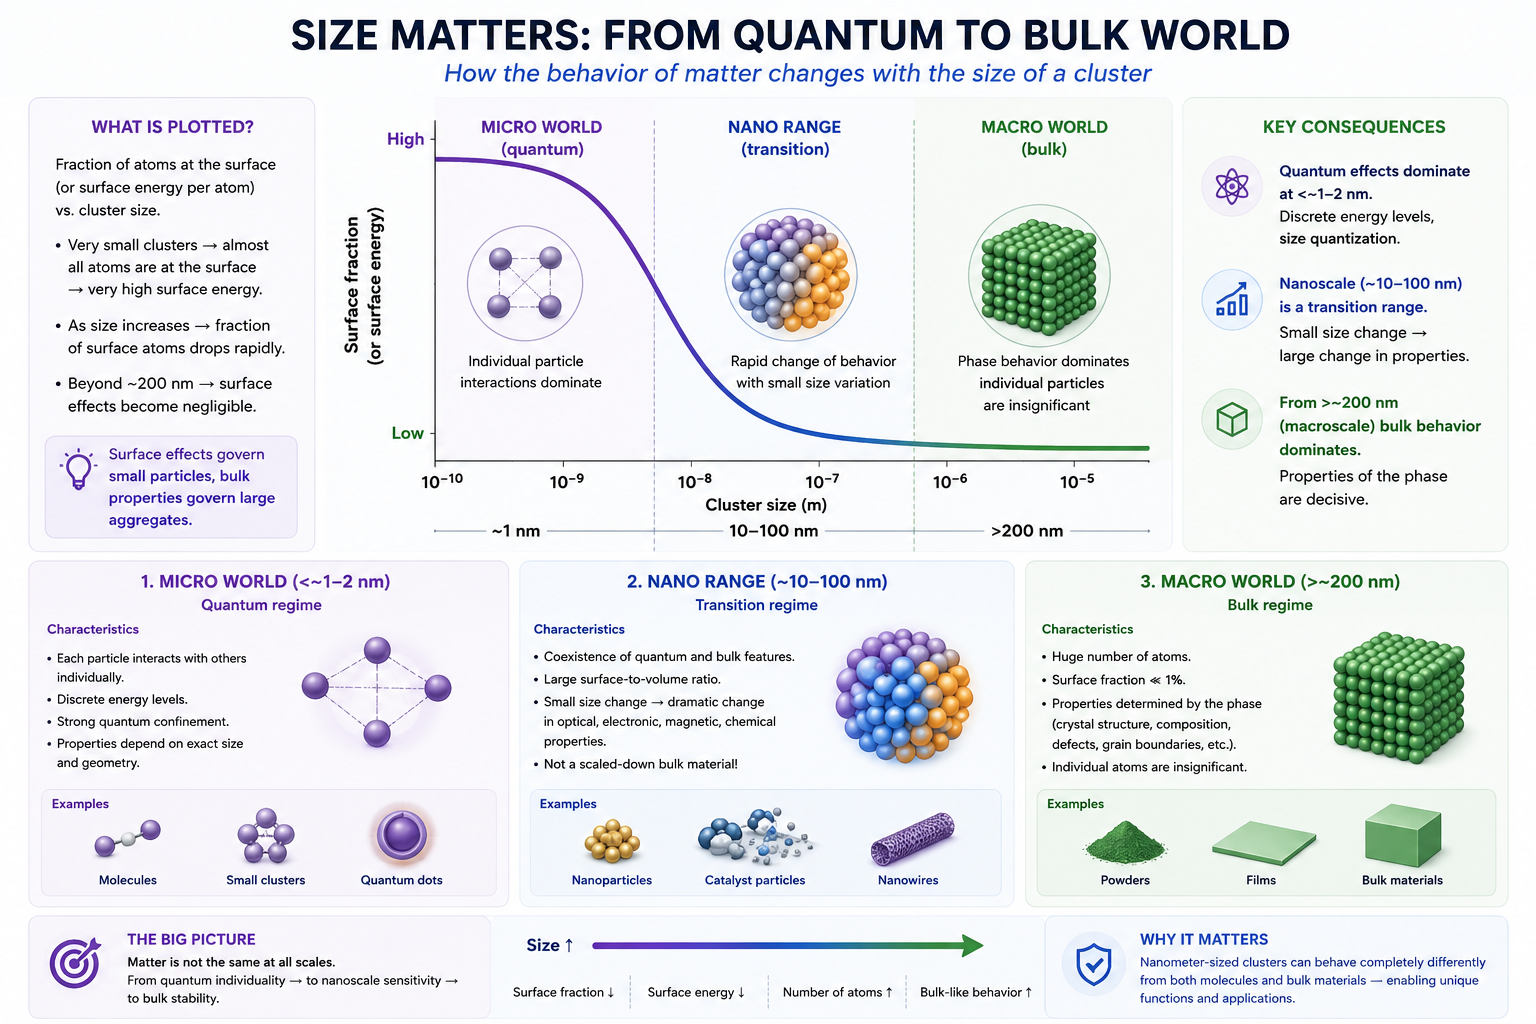
\includegraphics[keepaspectratio]{chapters/../images/image56.Nano.png}}
\#\#\# צבירה מול פיזור

מהמסקנות לעיל נובע:

\begin{itemize}
\tightlist
\item
  \textbf{צבירה} (aggregation) --- תהליך אטרקטיבי \textbf{אנרגטית}
  (מוריד אנרגיה)
\item
  \textbf{פיזור} (dispersion) --- תהליך אטרקטיבי \textbf{אנטרופית} (מעלה
  אנטרופיה)
\end{itemize}

שיווי המשקל בין שתי המגמות קובע את מצב הצבירה בטמפרטורה נתונה. בטמפרטורה
נמוכה --- האנרגיה שולטת, צבירה. בטמפרטורה גבוהה --- האנטרופיה שולטת,
פיזור. \#\# 7.4 מה קובע את מצב הצבירה?

\subsection{האנרגיה הקינטית מול אנרגיית
האינטראקציה}\label{ux5d4ux5d0ux5e0ux5e8ux5d2ux5d9ux5d4-ux5d4ux5e7ux5d9ux5e0ux5d8ux5d9ux5ea-ux5deux5d5ux5dc-ux5d0ux5e0ux5e8ux5d2ux5d9ux5d9ux5ea-ux5d4ux5d0ux5d9ux5e0ux5d8ux5e8ux5d0ux5e7ux5e6ux5d9ux5d4}

מצב הצבירה נקבע על ידי \textbf{היחס} בין שתי אנרגיות:

\begin{itemize}
\tightlist
\item
  \textbf{\(E_k\)} --- אנרגיה קינטית (תנועה תרמית, פרופורציונלית
  לטמפרטורה)
\item
  \textbf{\(E_\text{int}\)} --- אנרגיית האינטראקציה (עומק בור הפוטנציאל,
  תכונת החומר)
\end{itemize}

\[E_k \gg E_\text{int} \implies \textbf{gas}\]

\[E_k \approx E_\text{int} \implies \textbf{liquid}\]

\[E_k \ll E_\text{int} \implies \textbf{solid}\]

\textbf{גז:} החלקיקים עפים חופשי, מרחקים גדולים, כמעט אין אינטראקציה.

\textbf{נוזל:} כוחות ההתקשרות חזקים מספיק לשמור על המרחק, אבל לא מספיק
כדי לנעול מיקומים --- \textbf{זורם}.

\textbf{מוצק:} כוחות ההתקשרות נועלים כל חלקיק במיקומו ---
\textbf{נוקשה}. \#\# 7.5 צפיפות

\subsection{הגדרה
ומאפיינים}\label{ux5d4ux5d2ux5d3ux5e8ux5d4-ux5d5ux5deux5d0ux5e4ux5d9ux5d9ux5e0ux5d9ux5dd}

\[\rho = \frac{m}{V}, \qquad [\rho] = \text{kg/m}^3 \text{ , } \text{g/cm}^3\]

הצפיפות מאפיינת \textbf{כמה דחוסה האריזה} --- כמה מסה בנפח נתון.

\textbf{תלות בטמפרטורה:} ככל שהטמפרטורה עולה, המרחקים הבין-מולקולריים
גדלים → הנפח גדל → הצפיפות יורדת. חריג: מים בין \(0°C\) ל-\(4°C\) (ראו
להלן).

\textbf{תלות בלחץ:} גזים --- תלות חזקה (לחץ כפול = נפח חצי). נוזלים
ומוצקים --- תלות \textbf{זניחה} כמעט לחלוטין. לכן נוזלים ומוצקים נקראים
\textbf{פאזות מעובות} (condensed phases) --- אי אפשר לכווץ אותם משמעותית
על ידי לחץ.

\textbf{הבחנה: צפיפות אמיתית לעומת צפיפות נפחית}

כאשר חומר מוצק נמצא בצורת אבקה או גרגרים, בין הגרגרים נותרים
\textbf{חללים}. לכן:

\[\rho_\text{volume} = \rho_\text{true} \cdot (1 - \phi)\]

כאשר \(\phi = V_\text{pores}/V_\text{total}\) הוא \textbf{הנקבוביעות}
--- שבר הנפח של החללים, \(0 \leq \phi \leq 1\).

\textbf{דוגמה:} אבקת אלומינה (\(\text{Al}_2\text{O}_3\)) עם
\(\rho_\text{true} = 3.99\ \text{g/cm}^3\), אך לאחר מדידת נפח נפחי:
\(\rho_\text{volume} = 2.0\ \text{g/cm}^3\). הנקבוביעות \(\approx 0.5\)
--- חצי מהנפח הוא אוויר. \#\# 7.6 תכונות נוזלים

\subsection{זרימה --- מה הופך נוזל
לנוזל?}\label{ux5d6ux5e8ux5d9ux5deux5d4-ux5deux5d4-ux5d4ux5d5ux5e4ux5da-ux5e0ux5d5ux5d6ux5dc-ux5dcux5e0ux5d5ux5d6ux5dc}

הנוזל \textbf{אינו שומר על צורתו} --- כל כוח קטן גורם לזרימה. מדוע? כי
\(E_k \approx E_\text{int}\): כוחות ההתקשרות חזקים מספיק לשמור על מגע
בין המולקולות, אך לא מספיק לנעול אותן במיקום קבוע. כוח קטן מטה את האיזון
וגורם לתנועה.

\subsection{נפח קבוע --- מה הופך נוזל לשונה
מגז?}\label{ux5e0ux5e4ux5d7-ux5e7ux5d1ux5d5ux5e2-ux5deux5d4-ux5d4ux5d5ux5e4ux5da-ux5e0ux5d5ux5d6ux5dc-ux5dcux5e9ux5d5ux5e0ux5d4-ux5deux5d2ux5d6}

\textbf{הנפח של נוזל קבוע} (בתנאי לחץ קבוע) --- בניגוד לגז. הסיבה: כוחות
ון-דר-ולס שומרים על המרחקים הבין-מולקולריים בקירוב קבוע. הנוזל לוקח את
\textbf{צורת} הכלי --- אבל \textbf{לא את נפחו}.

\textbf{חריג: מים בין \(0°C\) ל-\(4°C\)}

מים \textbf{מתכווצים} כאשר מחממים מ-\(0°C\) ל-\(4°C\) --- כלומר, צפיפותם
\textbf{עולה} עם הטמפרטורה בטווח זה. בטמפרטורות מעל \(4°C\), ההתנהגות
חוזרת לרגילה.

הסיבה: בקרח, מולקולות המים מסודרות ברשת משושה עם מרחקים גדולים יחסית
(בשל קשרי מימן). כאשר הקרח נמס, חלק מהסדר הזה נשמר בצורת
\textbf{קלסטרים} (ראו §7.8). בחימום מ-\(0°C\) ל-\(4°C\), הקלסטרים
מתפרקים ומאפשרים ארגון צפוף יותר → הצפיפות עולה. מעל \(4°C\) שוב שולטת
ההתרחבות התרמית הרגילה.

\textbf{השלכה:} קרח \textbf{צף} על מים. זוהי תכונה חריגה --- רוב החומרים
המוצקים שוקעים בנוזל שלהם. הצפת הקרח מאפשרת לאגמים לשמור על מים נוזליים
מתחת לקרח בחורף, ומאפשרת חיים מימיים.

\subsection{צמיגות}\label{ux5e6ux5deux5d9ux5d2ux5d5ux5ea}

\textbf{צמיגות} \(\eta\) (viscosity) היא מדד \textbf{לחיכוך הפנימי}
בנוזל --- כמה קשה לגרום לשכבות הנוזל להחליק זו על גבי זו.

תיאור: \textbf{חוק פרנקל-אנדרד}:

\[\eta = \eta_0 \cdot e^{E_a / kT}\]

כאשר \(E_a\) היא אנרגיית השפעול לתנועת מולקולה (כמה אנרגיה נדרשת לה
``לברוח'' מסביבתה), \(k\) קבוע בולצמן, \(T\) טמפרטורה.

\textbf{המשמעות:} הצמיגות \textbf{יורדת אקספוננציאלית} עם עליית
הטמפרטורה --- מוכר מניסיון יומיומי (שמן חם זורם הרבה יותר בקלות מאשר שמן
קר; דבש חם לעומת דבש קר).

\textbf{נוזלים ניוטוניים לעומת לא-ניוטוניים:}

{\def\LTcaptype{none} % do not increment counter
\begin{longtable}[]{@{}
  >{\raggedright\arraybackslash}p{(\linewidth - 4\tabcolsep) * \real{0.1316}}
  >{\raggedright\arraybackslash}p{(\linewidth - 4\tabcolsep) * \real{0.4474}}
  >{\raggedright\arraybackslash}p{(\linewidth - 4\tabcolsep) * \real{0.4211}}@{}}
\toprule\noalign{}
\begin{minipage}[b]{\linewidth}\raggedright
סוג
\end{minipage} & \begin{minipage}[b]{\linewidth}\raggedright
הגדרה
\end{minipage} & \begin{minipage}[b]{\linewidth}\raggedright
דוגמאות
\end{minipage} \\
\midrule\noalign{}
\endhead
\bottomrule\noalign{}
\endlastfoot
ניוטוני & צמיגות קבועה, ללא תלות בקצב הגזירה & מים, שמן, אלכוהול \\
לא-ניוטוני & צמיגות תלויה בקצב הגזירה & קטשופ, שמפו, דם, בצק, עמילן
במים \\
\end{longtable}
}

\textbf{קטשופ} --- דוגמה קלאסית: כשלא מוזגים --- צמיג מאוד. כשמנערים
(מגדילים קצב גזירה) --- זורם. נוזלים כאלה נקראים \textbf{thixotropic}
(תיקסוטרופיים).

\textbf{עמילן במים} --- דוגמה הפוכה: ככל שמפעילים יותר כוח, נעשה
\textbf{יותר} צמיג (shear-thickening). לכן אם מניחים יד על המשטח בעדינות
--- שוקעים; אם מכים --- מקפצים. \#\# 7.7 מתח פנים, הרטבה ואפקט קפילרי

\subsection{מתח פנים --- מדוע נוזלים מעדיפים
להתכנס?}\label{ux5deux5eaux5d7-ux5e4ux5e0ux5d9ux5dd-ux5deux5d3ux5d5ux5e2-ux5e0ux5d5ux5d6ux5dcux5d9ux5dd-ux5deux5e2ux5d3ux5d9ux5e4ux5d9ux5dd-ux5dcux5d4ux5eaux5dbux5e0ux5e1}

כל מולקולה בתוך נוזל מוקפת שכנות מכל הכיוונים ומושכת על ידיהן שווה.
מולקולה על \textbf{פני השטח} --- מוקפת שכנות רק מהצד הפנימי, ולכן נמשכת
\textbf{פנימה}. כתוצאה:

\begin{itemize}
\tightlist
\item
  מולקולות שטח נמצאות \textbf{באנרגיה גבוהה יותר} מאשר מולקולות הגוש
\item
  הנוזל \textbf{מנסה למזער} את שטח פניו (לצמצם מספר מולקולות השטח)
\end{itemize}

\textbf{מתח הפנים} \(\gamma\) מוגדר כאנרגיה ליחידת שטח:
\([\gamma] = \text{J/m}^2 = \text{N/m}\).

\textbf{תופעות:} טיפות מים כדוריות (כדור --- שטח מינימלי לנפח נתון). מחט
פלדה ``שוכבת'' על מים (משקלה קטן מהכוח שמפעיל מתח הפנים). חרקי מים
הולכים על פני מים.

\textbf{גורמים המורידים מתח פנים --- סורפקטנטים (חפ''ש)}

\textbf{חומרים פעילי שטח} (surfactants; בעברית: חפ''ש = חומר פעיל שטח)
הם מולקולות עם שני קצוות: קצה \textbf{הידרופילי} (מושך מים) וקצה
\textbf{הידרופובי} (דוחה מים). הן מסתדרות על פני השטח כשהקצה ההידרופילי
בתוך המים והקצה ההידרופובי מבחוץ --- ובכך \textbf{מפחיתות את מתח הפנים}.

\textbf{דוגמאות:} סבון, שמפו, אבקת כביסה, חומרי ניקוי. הורדת מתח הפנים
מאפשרת למים ``להתפשט'' על לכלוך ולהרטיב אותו --- עיקרון הניקוי.

\subsection{הרטבה וזווית
המגע}\label{ux5d4ux5e8ux5d8ux5d1ux5d4-ux5d5ux5d6ux5d5ux5d5ux5d9ux5ea-ux5d4ux5deux5d2ux5e2}

כאשר טיפה נוזל מונחת על משטח, הצורה שהיא מקבלת תלויה בשלושה מתחי פנים:
נוזל-גז, מוצק-גז, ומוצק-נוזל. \textbf{זווית המגע} \(\theta\) היא הזווית
הנוצרת בין הטיפה לפני המשטח:

{\def\LTcaptype{none} % do not increment counter
\begin{longtable}[]{@{}
  >{\raggedright\arraybackslash}p{(\linewidth - 6\tabcolsep) * \real{0.2000}}
  >{\raggedright\arraybackslash}p{(\linewidth - 6\tabcolsep) * \real{0.2762}}
  >{\raggedright\arraybackslash}p{(\linewidth - 6\tabcolsep) * \real{0.1810}}
  >{\raggedright\arraybackslash}p{(\linewidth - 6\tabcolsep) * \real{0.3429}}@{}}
\toprule\noalign{}
\begin{minipage}[b]{\linewidth}\raggedright
זווית
\end{minipage} & \begin{minipage}[b]{\linewidth}\raggedright
שם
\end{minipage} & \begin{minipage}[b]{\linewidth}\raggedright
משמעות
\end{minipage} & \begin{minipage}[b]{\linewidth}\raggedright
דוגמה
\end{minipage} \\
\midrule\noalign{}
\endhead
\bottomrule\noalign{}
\endlastfoot
\(\theta < 90°\) & \textbf{ליאופילי} (מים: הידרופילי) & הרטבה טובה & מים
על זכוכית (\(\theta \approx 38°\)) \\
\(\theta > 90°\) & \textbf{ליאופובי} (מים: הידרופובי) & הרטבה גרועה &
מים על טפלון (\(\theta \approx 98°\)) \\
\(\theta \approx 0°\) & הרטבה מלאה & הנוזל מתפשט לחלוטין & --- \\
\(\theta \approx 180°\) & דחייה מלאה & טיפה כדורית מושלמת & ``גיליון
לוטוס'' \\
\end{longtable}
}

\textbf{אפקט לוטוס:} עלים של צמח הלוטוס בעלי מיקרו-מבנה המיצר
הידרופוביות קיצונית (\(\theta > 150°\)) --- טיפות מים מגלגלות ולוקחות
עמן לכלוך. השראה לחומרים מנקים עצמית.

\subsection{אפקט
קפילרי}\label{ux5d0ux5e4ux5e7ux5d8-ux5e7ux5e4ux5d9ux5dcux5e8ux5d9}

בצינור דק (קפילרה), מתח הפנים גורם לנוזל לעלות (אם הידרופילי) או לרדת
(אם הידרופובי) ביחס לגובה הנוזל החיצוני:

\[h = \frac{2\gamma \cos\theta}{r(\rho - \rho_0)g}\]

כאשר:

\begin{itemize}
\tightlist
\item
  \(h\) --- גובה העלייה/ירידה {[}m{]}
\item
  \(\gamma\) --- מתח פנים \([\text{N/m}]\)
\item
  \(\theta\) --- זווית המגע
\item
  \(r\) --- רדיוס הקפילרה {[}m{]}
\item
  \(\rho\) --- צפיפות הנוזל \([\text{kg/m}^3]\)
\item
  \(\rho_0\) --- צפיפות הגז מעל הנוזל (בדרך כלל זניחה)
\item
  \(g = 9.8\ \text{m/s}^2\)
\end{itemize}

בתנאי הרטבה מלאה (\(\cos\theta \approx 1\)):

\[h \approx \frac{2\gamma}{r\rho g}\]

\textbf{שימו לב:} ככל שהצינור \textbf{דק יותר} (\(r\) קטן יותר), הנוזל
עולה \textbf{גבוה יותר}. זה ההסבר לעלייה של מים בצמחים דרך כלי הצנרה
העדינים שלהם (קוטר \(\sim 10^{-5}\ \text{m}\)), לספיגה בנייר, ולחדירת
מים בסלעים פורוזיים.

\begin{quote}
\textbf{תרגיל:} מים (\(\gamma = 0.073\ \text{N/m}\),
\(\rho = 1000\ \text{kg/m}^3\)) בצינור זכוכית עם \(r = 0.1\ \text{mm}\).
חשבו את גובה העלייה. (תשובה: \(\approx 15\ \text{cm}\))
\end{quote}

\pandocbounded{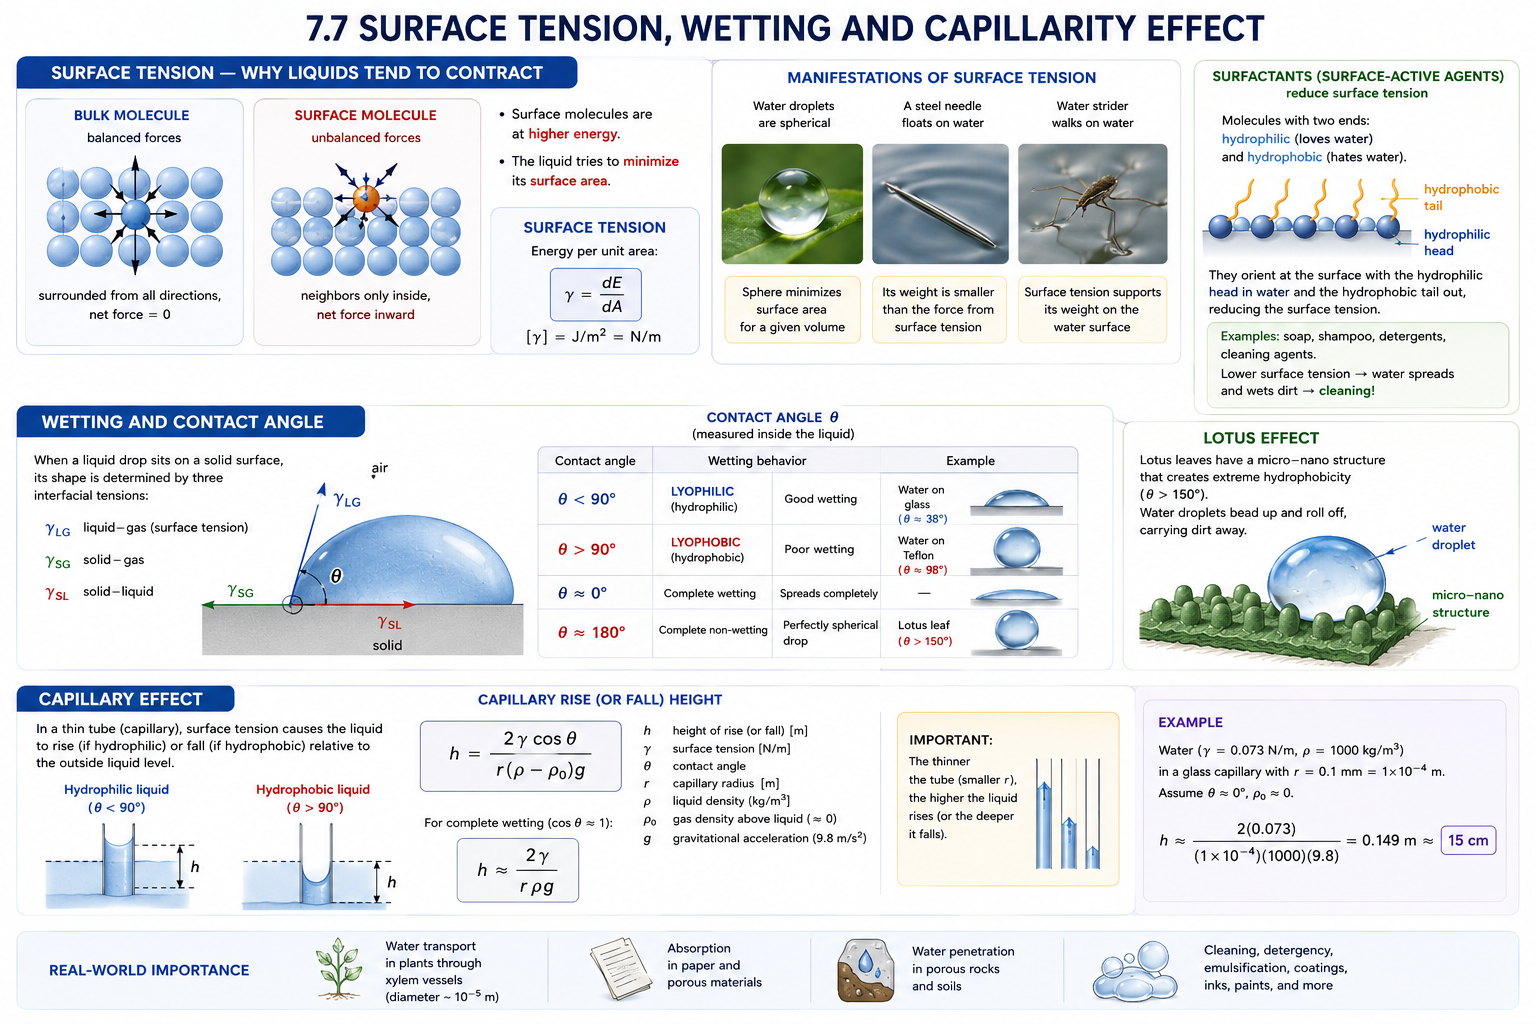
\includegraphics[keepaspectratio]{chapters/../images/image57.SurfaceTension.png}}
\#\# 7.8 מודל הקלסטרים --- מה קורה בתוך נוזל?

\subsection{נוזל --- מצב
ביניים}\label{ux5e0ux5d5ux5d6ux5dc-ux5deux5e6ux5d1-ux5d1ux5d9ux5e0ux5d9ux5d9ux5dd}

נוזל אינו לא-מוצק ולא לא-גז --- הוא מצב \textbf{עצמאי} עם מאפיינים
ייחודיים. כדי להבין אותו, נשתמש ב\textbf{מודל הקלסטרים}:

\textbf{בנוזל קיימים קלסטרים} (clusters) --- אזורים בגודל עשרות עד מאות
מולקולות שבהם קיים \textbf{סדר מקומי} דמוי מוצק, שוקעים בתוך ``ים''
אקראי.

{\def\LTcaptype{none} % do not increment counter
\begin{longtable}[]{@{}lll@{}}
\toprule\noalign{}
חומר & מצב & תיאור \\
\midrule\noalign{}
\endhead
\bottomrule\noalign{}
\endlastfoot
מוצק & סדר רחוק-טווח מלא & כל אטום במיקום קבוע \\
נוזל & סדר קצר-טווח בלבד & קלסטרים מסודרים, אקראי בין הקלסטרים \\
גז & אין סדר & אקראי לחלוטין \\
\end{longtable}
}

\textbf{ככל שהטמפרטורה עולה:}

\begin{itemize}
\tightlist
\item
  הקלסטרים קטנים וקצרי-חיים יותר
\item
  שבר האזורים האקראיים גדל
\item
  הנוזל ``נעשה יותר כמו גז''
\end{itemize}

\textbf{בדיוק בגלל זה} ניסי שטרן-גרלך-פוכ על מים מראים שיחסי השכנות
הממוצעים בין מולקולות מים קרובים לאלה שבקרח --- קיים עדיין ``זיכרון''
מבני חלקי. \#\# 7.9 המצב האמורפי

\subsection{מוצק שאינו
גביש}\label{ux5deux5d5ux5e6ux5e7-ux5e9ux5d0ux5d9ux5e0ux5d5-ux5d2ux5d1ux5d9ux5e9}

כאשר נוזל מצונן \textbf{מהר מאוד}, הקלסטרים הקיימים ``מוקפאים'' במקומם
לפני שהמולקולות מספיקות לסדר עצמן לרשת גבישית מסודרת. התוצאה היא
\textbf{מצב אמורפי} (amorphous) --- מוצק ללא סדר רחוק-טווח.

\textbf{דוגמאות:} זכוכית (SiO₂ מצונן), מתכות אמורפיות (metallic
glasses), פולימרים מסוימים.

\subsection{הבדלים בין גביש
לאמורפי}\label{ux5d4ux5d1ux5d3ux5dcux5d9ux5dd-ux5d1ux5d9ux5df-ux5d2ux5d1ux5d9ux5e9-ux5dcux5d0ux5deux5d5ux5e8ux5e4ux5d9}

{\def\LTcaptype{none} % do not increment counter
\begin{longtable}[]{@{}lll@{}}
\toprule\noalign{}
תכונה & גביש & אמורפי \\
\midrule\noalign{}
\endhead
\bottomrule\noalign{}
\endlastfoot
סדר מבני & רחוק-טווח מלא & קצר-טווח בלבד \\
מצב תרמודינמי & \textbf{שיווי משקל} & \textbf{לא שיווי משקל} \\
טמפרטורת התכה & מוגדרת חדה (\(T_m\)) & \textbf{אין} --- רכות הדרגתית \\
צמיגות & קופצת בחדות ב-\(T_m\) & יורדת \textbf{בהדרגה} עם \(T\) \\
\end{longtable}
}

\textbf{המצב האמורפי הוא מצב לא שיווי משקל} --- אם ממתינים מספיק זמן (או
מחממים), החומר יתגבש לחלוטין. ``מספיק זמן'' יכול להיות שניות (עבור מתכות
נוזליות) עד מיליוני שנים (עבור זכוכית אורגנית). האגדה על ``זכוכיות
הקתדרלה שהתעבו למטה עם השנים'' --- לא נכון; זכוכיות עתיקות הן עבות יותר
בתחתית בשל אופן הייצור הידני, לא בשל זרימה.

\subsection{טמפרטורת המעבר
הזגוגי}\label{ux5d8ux5deux5e4ux5e8ux5d8ux5d5ux5e8ux5ea-ux5d4ux5deux5e2ux5d1ux5e8-ux5d4ux5d6ux5d2ux5d5ux5d2ux5d9}

אמנם לחומר אמורפי אין \(T_m\) חד, אבל יש \textbf{טמפרטורת מעבר זגוגי}
\(T_g\) (glass transition temperature) --- טמפרטורה שמתחתיה החומר מוצק
קשיח ומעליה הוא רך ופלסטי. המעבר אינו חד כמו התכה --- זהו שינוי הדרגתי
בצמיגות.

\textbf{יישומים:}

\begin{itemize}
\tightlist
\item
  \textbf{מתכות אמורפיות} --- קשיחות מאוד ועמידות בפני שחיקה; משמשות
  ברקורדרי קלטת מגנטית ובראשי גילוח.
\item
  \textbf{זכוכיות מיוחדות} --- מוליכי אור, חלונות לייזר.
\item
  \textbf{פולימרים} --- \(T_g\) קובעת אם הפלסטיק קשיח (מתחת ל-\(T_g\))
  או גמיש (מעליה) בטמפרטורת שימוש. \#\# סיכום
\end{itemize}

שבעה נושאים עיקריים:

\textbf{מיקרוסקופי מול מאקרוסקופי} --- תכונות מאקרוסקופיות מוגדרות לפאזה
(אוסף גדול), לא לחלקיק בודד.

\textbf{פוטנציאל לנארד-ג'ונס} --- שילוב דחייה (\(r^{-12}\)) ומשיכה
(\(r^{-6}\)) נותן בור פוטנציאל. אטום בחומר יציב יותר מאשר בוואקום.

\textbf{שטח מול גוש} --- חלקיקי שטח באנרגיה גבוהה יותר. ננוחלקיקים ---
רוב האטומים הם שטח → תכונות שונות מגוש.

\textbf{מצב הצבירה} --- נקבע לפי \(E_k/E_\text{int}\): גז (גדול), נוזל
(דומה), מוצק (קטן).

\textbf{צמיגות} --- פרנקל-אנדרד: \(\eta = \eta_0 e^{E_a/kT}\). יורדת עם
חימום. ניוטוני מול לא-ניוטוני.

\textbf{מתח פנים, הרטבה, קפילריות} --- כוחות ון-דר-ולס על פני שטח גורמים
לכל התופעות הללו. \(h = 2\gamma\cos\theta/(r\rho g)\).

\textbf{קלסטרים ומצב אמורפי} --- נוזל = קלסטרים על רקע אקראי. קירור מהיר
= קיפאון מבני = מצב אמורפי (לא שיווי משקל).

\bookmarksetup{startatroot}

\chapter{פרק 8 --- מבנה מוצקים: אריזות, מבנים
ומעברים}\label{ux5e4ux5e8ux5e7-8-ux5deux5d1ux5e0ux5d4-ux5deux5d5ux5e6ux5e7ux5d9ux5dd-ux5d0ux5e8ux5d9ux5d6ux5d5ux5ea-ux5deux5d1ux5e0ux5d9ux5dd-ux5d5ux5deux5e2ux5d1ux5e8ux5d9ux5dd}

\section{מבוא: מדוע מוצקים
מעניינים?}\label{ux5deux5d1ux5d5ux5d0-ux5deux5d3ux5d5ux5e2-ux5deux5d5ux5e6ux5e7ux5d9ux5dd-ux5deux5e2ux5e0ux5d9ux5d9ux5e0ux5d9ux5dd}

מדע החומרים הוא במידה רבה מדע המוצקים. כל הרכיבים האלקטרוניים, כל חומרי
הבנייה, כל כלי הנשק וכל המנועים --- עשויים מוצקים. \textbf{תכונות} המוצק
--- קשיות, הולכה חשמלית, עמידות לחום, מגנטיות --- נקבעות ישירות על ידי
\textbf{מבנה גבישי} שלו: כיצד האטומים מסודרים, כיצד הם קשורים, ואיזה
פגמים קיימים.

פרק זה בונה את הכלים להבנת מבנה מוצקים, מהגיאומטריה הפשוטה של כדורים ועד
לתורת שדה הגביש ומעברים פולימורפיים. \#\# חלק א': גיאומטריה של אריזות
--- בסיס הכל \#\# 8.1 אריזת כדורים במישור

\subsection{מדוע להתחיל
בכדורים?}\label{ux5deux5d3ux5d5ux5e2-ux5dcux5d4ux5eaux5d7ux5d9ux5dc-ux5d1ux5dbux5d3ux5d5ux5e8ux5d9ux5dd}

אטומים במוצק אינם מרובעים ואינם מצולעים --- הם (בקירוב) \textbf{כדורים}.
השאלה הגיאומטרית הבסיסית: \textbf{מה הדרך הדחוסה ביותר לאחסן כדורים
זהים?} התשובה לשאלה זו קובעת את מבני המתכות והקרמיקה.

\subsection{שכבה אחת}\label{ux5e9ux5dbux5d1ux5d4-ux5d0ux5d7ux5ea}

שלושה כדורים זהים בצמוד זה לזה יוצרים משולש שווה-צלעות --- ממש הדרך הכי
דחוסה. אם ממשיכים ומוסיפים כדורים, כל כדור מוקף בשישה כדורים ---
\textbf{מוטיב משושה}. זה מתקבל אוטומטית מגיאומטריה טהורה, ללא ``תכנון''.

בין הכדורים נשארים \textbf{חללים} (voids). בשכבה דו-ממדית קיימים שני
סוגים:

\begin{itemize}
\tightlist
\item
  \textbf{וויד T} (Tetrahedral void): החלל שנוצר כאשר שלושה כדורים
  יוצרים משולש ולחלל יש כיוון ``מחודד''
\item
  \textbf{וויד ⊥} (Octahedral void): החלל בצורה הפוכה
\end{itemize}

\textbf{כלל:} על כל כדור בשכבה --- וויד T אחד ווויד ⊥ אחד.

\subsection{שתי שכבות}\label{ux5e9ux5eaux5d9-ux5e9ux5dbux5d1ux5d5ux5ea}

כאשר מניחים שכבה שנייה (B) על שכבה קיימת (A), כדורי B \textbf{נופלים
בדיוק לתוך} וואידי שכבה A. לא משנה אם על T-void או ⊥-void --- התוצאה זהה
(ניתן להמיר ביניהן בסיבוב \(180°\)). לכן: \(AB = BA\).

תוצאה חשובה: תחת \textbf{מחצית} וואידי שכבה B יושבים כדורי שכבה A; תחת
המחצית השנייה --- וואידי שכבה A. עובדה זו תהיה מפתח לסיווג הוואידים
התלת-ממדיים.

\subsection{שלוש שכבות: FCC
ו-HCP}\label{ux5e9ux5dcux5d5ux5e9-ux5e9ux5dbux5d1ux5d5ux5ea-fcc-ux5d5-hcp}

כאשר מניחים שכבה שלישית, קיימות בדיוק \textbf{שתי אפשרויות}:

\textbf{סידור ABA (ABABAB\ldots):} השכבה השלישית ממוקמת \textbf{מעל}
כדורי שכבה A. → \textbf{HCP} (Hexagonal Close Packing = אריזה צפופה
משושה)

\textbf{סידור ABC (ABCABC\ldots):} השכבה השלישית ממוקמת מעל
\textbf{וואידי} שכבה A (מיקום חדש לחלוטין). → \textbf{FCC}
(Face-Centered Cubic = קובי-פנים-מרוכז)

\textbf{אין אפשרות שלישית} --- זה הוכח מתמטית.

שתי האריזות שוות ב\textbf{אחוז האריזה}: 74\% מהנפח תפוס בכדורים, 26\%
חללים. זוהי \textbf{האריזה הצפופה ביותר האפשרית} (משפט קפלר, הוכח ב-1998
על ידי מחשב).
\pandocbounded{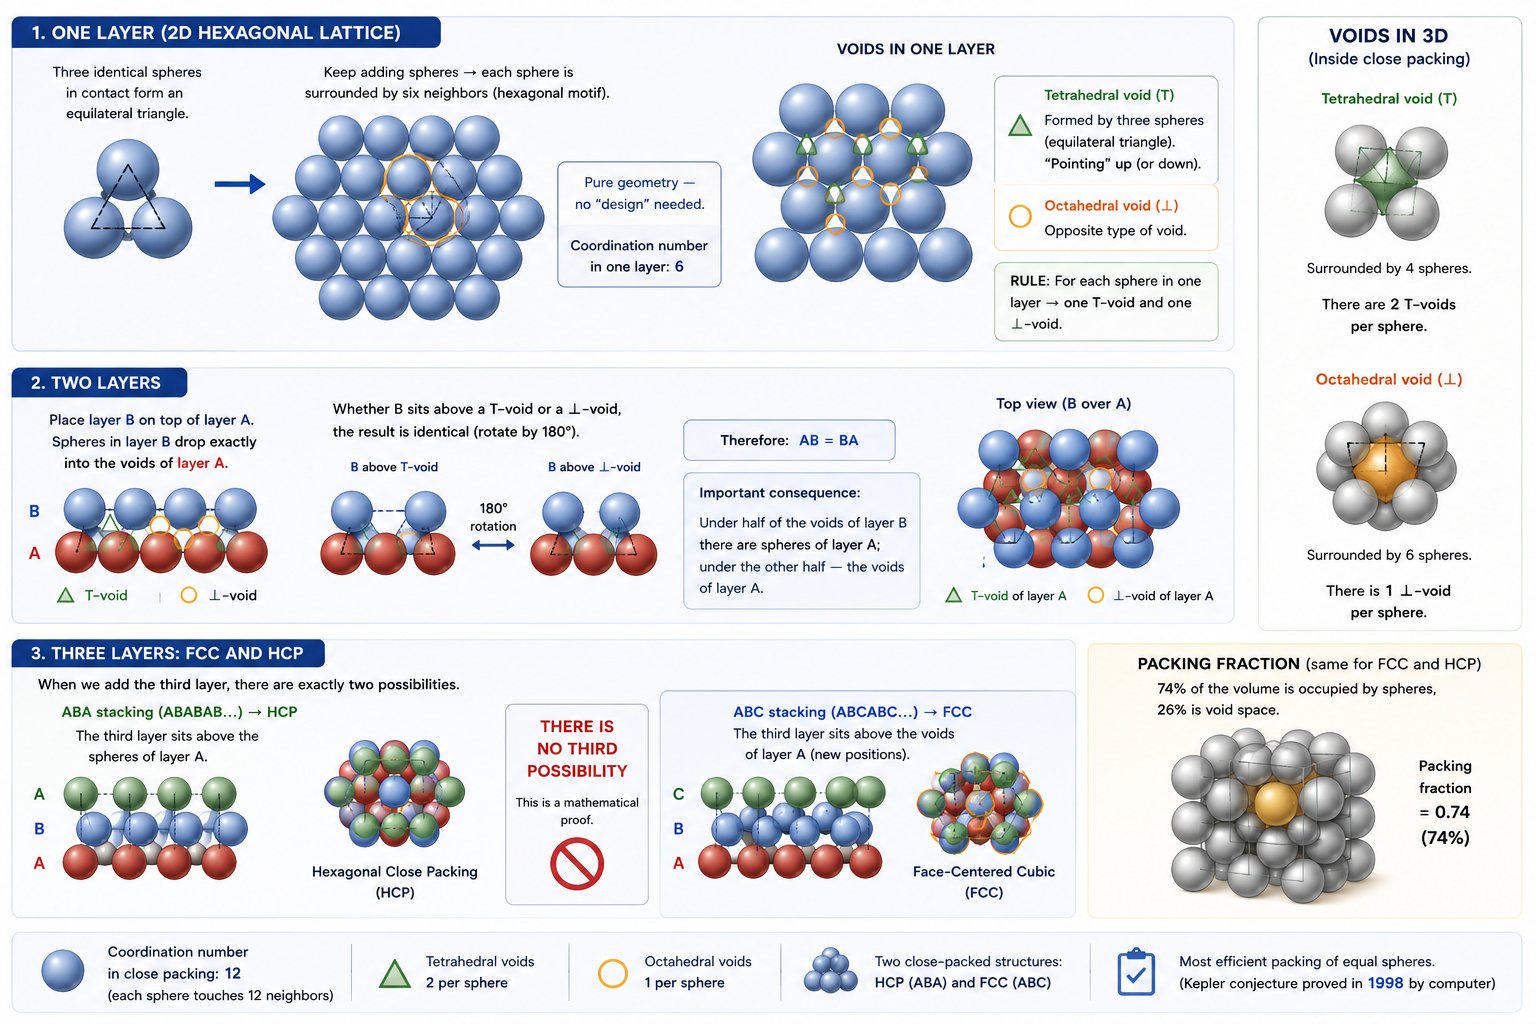
\includegraphics[keepaspectratio]{chapters/../images/image58.rigidSpheres.png}}
\#\# 8.2 וואידים בתלת-ממד

\subsection{שני סוגי
וואידים}\label{ux5e9ux5e0ux5d9-ux5e1ux5d5ux5d2ux5d9-ux5d5ux5d5ux5d0ux5d9ux5d3ux5d9ux5dd}

בכל אריזה צפופה (FCC או HCP) קיימים שני סוגי חללים:

\textbf{וויד טטרהדרלי} (T-void): נוצר כאשר כדור אחד מונח מעל שלושה
כדורים בשכבה מתחת. ארבעת הכדורים יוצרים \textbf{טטרהדרון} (פירמידה
משולשת). החלל קטן יחסית, הגודל (אורך הצלע) שלו הוא 0.225 של רדיוס הכדור
והנפח שלו הוא כ-1.1\% של נפח הכדור.

\textbf{וויד אוקטהדרלי} (O-void): נוצר כאשר שלושה כדורים משכבה אחת
נפגשים עם שלושה כדורים משכבה שנייה. ששת הכדורים יוצרים
\textbf{אוקטהדרון}. החלל גדול יותר --- הרדיוס (המרחק בין שני קודקודים
הפוכים) הוא 0.414 של רדיוס הכדור ונפחו בערך 41\% מנפח הכדור.

\subsection{הכלל המרכזי (ללא
הוכחה)}\label{ux5d4ux5dbux5dcux5dc-ux5d4ux5deux5e8ux5dbux5d6ux5d9-ux5dcux5dcux5d0-ux5d4ux5d5ux5dbux5d7ux5d4}

\textbf{על כל אטום} באריזה צפופה, בין FCC ובין HCP, ישנם תמיד 2 וואידים
טטרהדרליים + 1 וויד אוקטהדרלי

כלל זה הוא \textbf{יסוד} להבנת מבנים יוניים: הוא קובע כמה יונים קטנים
יכולים להיכנס לרשת של יונים גדולים. \#\# 8.3 מודל הכדורים הקשיחים ---
ישימות ומגבלות

\subsection{מתי המודל
עובד?}\label{ux5deux5eaux5d9-ux5d4ux5deux5d5ux5d3ux5dc-ux5e2ux5d5ux5d1ux5d3}

\textbf{מודל הכדורים הקשיחים} --- מניח שאטומים/יונים הם כדורים קשיחים
ובלתי-דחיסים --- עובד היטב כאשר:

\begin{itemize}
\tightlist
\item
  \textbf{מתכות:} מבניהן מתוארים מצוין. כמעט כל המתכות FCC, HCP, או BCC.
\item
  \textbf{חומרים יוניים:} כאשר הפרש הרדיוסים גדול, הכדורים הגדולים
  (אניונים) יוצרים אריזה והקטנים (קטיונים) נכנסים לוואידים.
\end{itemize}

\subsection{מגבלות}\label{ux5deux5d2ux5d1ux5dcux5d5ux5ea}

המודל \textbf{אינו} מסביר:

\begin{itemize}
\tightlist
\item
  \textbf{מדוע} מתכת מסוימת בוחרת FCC ואחרת HCP (שתיהן אריזות שוות!)
\item
  \textbf{אלוטרופיה} של ברזל: \(\text{Fe}\) בטמפרטורה רגילה הוא BCC
  (פחות צפוף!), מעל \(912°C\) --- FCC, ואז שוב BCC לפני ההיתוך. לפי
  הגיון הכדורים, הצפוף צריך להיות יציב --- אך לא תמיד כך.
\item
  \textbf{מעברים מרטנזיטיים} ותופעות קוונטיות בסריג
\end{itemize}

לבעיות אלו צריך מודל מורכב יותר --- מנגנוניים קוונטיים, תורת פסי אנרגיה
(band theory). \#\# חלק ב': מבנים יוניים --- קרמיקה ותרכובות \#\# 8.4
עקרון המבנה היוני

\subsection{הרעיון}\label{ux5d4ux5e8ux5e2ux5d9ux5d5ux5df-2}

\textbf{חומרים יוניים} --- תחמוצות, גופריתות, הלוגנידים --- מורכבים
מיונים עם מטענים הפוכים. \textbf{אניונים} (מטען שלילי) בדרך כלל
\textbf{גדולים} יותר; \textbf{קטיונים} (מטען חיובי) בדרך כלל
\textbf{קטנים} יותר.

\textbf{מדוע?} כאשר אטום מאבד אלקטרונים (קטיון חיובי), הגרעין מושך את
הנותרים חזק יותר → מתכווץ. כאשר מקבל (אניון שלילי) → מתרחב.

\textbf{מודל:} האניונים הגדולים יוצרים אריזה צפופה (FCC או HCP),
והקטיונים הקטנים מתמקמים בוואידים.

\subsection{חוקי
פולינג}\label{ux5d7ux5d5ux5e7ux5d9-ux5e4ux5d5ux5dcux5d9ux5e0ux5d2}

ב-1929 ניסח \textbf{ליינוס פולינג} (זוכה פרס נובל בכימיה 1954, ובשלום
1962 --- היחיד שזכה פעמיים בנפרד) חמישה כללים לחיזוי מבני גבישים יוניים.

\subsubsection{חוק ראשון: פאון
הקואורדינציה}\label{ux5d7ux5d5ux5e7-ux5e8ux5d0ux5e9ux5d5ux5df-ux5e4ux5d0ux5d5ux5df-ux5d4ux5e7ux5d5ux5d0ux5d5ux5e8ux5d3ux5d9ux5e0ux5e6ux5d9ux5d4}

סביב כל קטיון נוצר \textbf{פאון קואורדינציה} (polyhedron) של אניונים.
מספר הקואורדינציה (CN) נקבע על ידי \textbf{יחס הרדיוסים} \(r_c/r_a\):

{\def\LTcaptype{none} % do not increment counter
\begin{longtable}[]{@{}lll@{}}
\toprule\noalign{}
\(r_c/r_a\) & CN & גיאומטריה \\
\midrule\noalign{}
\endhead
\bottomrule\noalign{}
\endlastfoot
\(< 0.155\) & 2 & קווי \\
\(0.155\)--\(0.225\) & 3 & משולש \\
\(0.225\)--\(0.414\) & 4 & \textbf{טטרהדרון} \\
\(0.414\)--\(0.732\) & 6 & \textbf{אוקטהדרון} \\
\(0.732\)--\(1.00\) & 8 & קובייה \\
\(1.00\) & 12 & קובוקטהדרון \\
\end{longtable}
}

\textbf{ההיגיון:} ככל שהקטיון גדול יותר ביחס לאניון, יש מקום ליותר
אניונים סביבו. הטבלה מגיעה מחישוב גיאומטרי טהור: מה הרדיוס המינימלי של
כדור שיכול לשבת בתוך \(n\) כדורים בצמוד?

\subsubsection{חוק שני: ערכיות
אלקטרוסטטית}\label{ux5d7ux5d5ux5e7-ux5e9ux5e0ux5d9-ux5e2ux5e8ux5dbux5d9ux5d5ux5ea-ux5d0ux5dcux5e7ux5d8ux5e8ux5d5ux5e1ux5d8ux5d8ux5d9ux5ea}

מבנה יוני יציב כאשר: \[z_c \times CN_c = z_a \times CN_a\]

כאשר \(z\) הוא מטען היון ו-\(CN\) הוא מספר הקואורדינציה.

\textbf{דוגמה --- NaCl:} \(\text{Na}^+\) (מטען +1) מוקף ב-6
\(\text{Cl}^-\); כל \(\text{Cl}^-\) (מטען -1) מוקף ב-6 \(\text{Na}^+\).
\(1 \times 6 = 1 \times 6\) ✓

\textbf{דוגמה --- MgO:} \(\text{Mg}^{2+}\) (מטען +2) מוקף ב-6
\(\text{O}^{2-}\); \(2 \times 6 = 2 \times 6\) ✓

\subsubsection{חוק שלישי: אי-שיתוף
פנים}\label{ux5d7ux5d5ux5e7-ux5e9ux5dcux5d9ux5e9ux5d9-ux5d0ux5d9-ux5e9ux5d9ux5eaux5d5ux5e3-ux5e4ux5e0ux5d9ux5dd}

שיתוף \textbf{פנים} בין שני פאוני קואורדינציה \textbf{מפחית יציבות} ---
הקטיונים בשני הפאונים מתקרבים ודוחים זה את זה. שיתוף \textbf{צלעות} ---
פחות גרוע. שיתוף \textbf{קודקודים בלבד} --- היציב ביותר.

\textbf{דוגמה:} שני טטרהדרות של \(\text{SiO}_4\) לעולם לא חולקות פנים
ולרוב לא צלעות --- רק קודקודים. לכן ב-\(\text{SiO}_2\) כל ה-O גשריים
(Si-O-Si). זו הסיבה שהסיליקטים (המינרלים הנפוצים ביותר על פני הארץ) כל
כך מגוונים.

\subsubsection{חוקים רביעי
וחמישי}\label{ux5d7ux5d5ux5e7ux5d9ux5dd-ux5e8ux5d1ux5d9ux5e2ux5d9-ux5d5ux5d7ux5deux5d9ux5e9ux5d9}

\textbf{חוק רביעי:} קטיונים עם מטען גבוה ו-CN נמוך לא חולקים אלמנטים בין
פאוניהם.

\textbf{חוק חמישי (חוק הפשטות):} מספר סוגי המיקומים בגביש נוטה להיות קטן
--- גבישים פשוטים בדרך כלל.
\pandocbounded{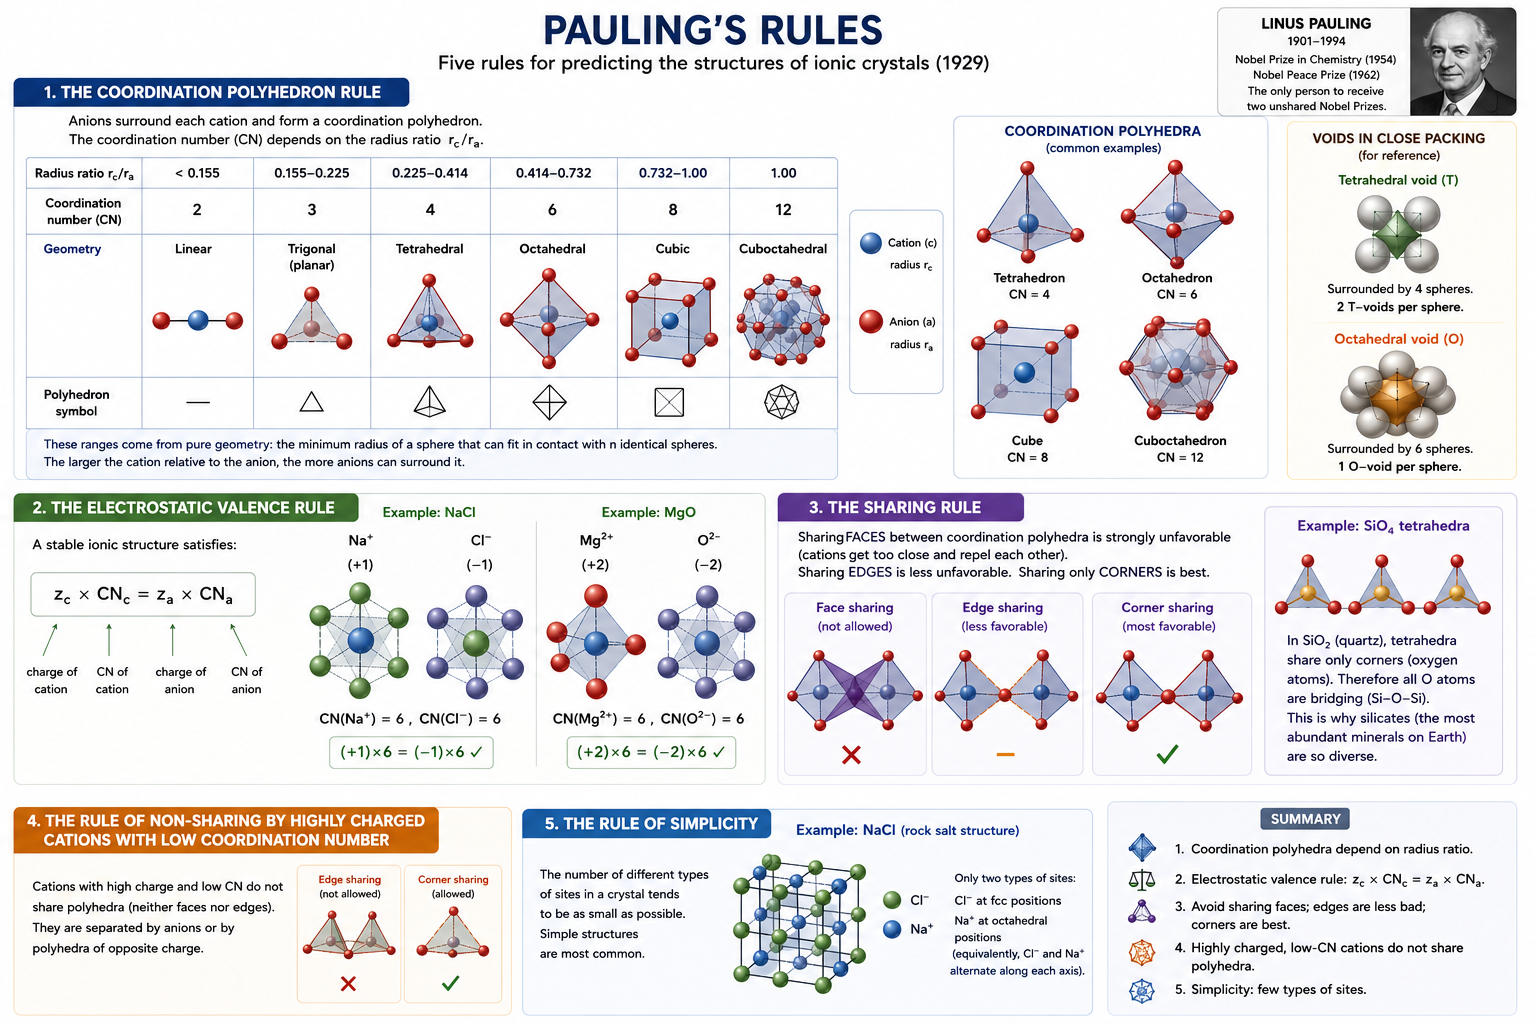
\includegraphics[keepaspectratio]{chapters/../images/image59.PaulingRules.png}}
\#\# 8.5 מבנים יוניים בסיסיים

\subsection{AX --- מלח סלע
(NaCl)}\label{ax-ux5deux5dcux5d7-ux5e1ux5dcux5e2-nacl}

\textbf{דוגמאות:} NaCl, LiF, MgO, CaO, SrO, BaO, FeO, NiO

כל האוקסידים בסיסיים של מתכות אלקליות-עפרות (MgO, CaO\ldots) הם במבנה
מלח סלע --- חשוב לתעשייה (חומרי עמידות חום).

\textbf{מבנה:} FCC של \(\text{Cl}^-\), עם \(\text{Na}^+\) בכל הוואידים
האוקטהדרליים.

\textbf{מוטיב:} \(\text{Cl}\) ב-\((0,0,0)\); \(\text{Na}\)
ב-\((\frac{1}{2},0,0)\)

\textbf{נתונים:} 4 יחידות NaCl בתא יחידה; \(0.414 < r_c/r_a < 0.732\);
קואורדינציה 6:6 (אוקטהדרלית).

\begin{quote}
\textbf{לחשיבה:} מגנזיה (MgO) היא חומר עמידות חום נפוץ. טמפרטורת ההיתוך
שלה: \(2852°C\). מדוע גבוהה כל כך? (רמז: מטענים +2 ו-−2 לעומת +1 ו-−1
ב-NaCl)
\end{quote}

\subsection{AX --- ציזיום כלוריד
(CsCl)}\label{ax-ux5e6ux5d9ux5d6ux5d9ux5d5ux5dd-ux5dbux5dcux5d5ux5e8ux5d9ux5d3-cscl}

\textbf{דוגמאות:} CsCl, TlBr, \(\text{NH}_4\text{Cl}\) בלחץ גבוה

\textbf{מבנה:} סריג פרימיטיבי קובי --- \textbf{לא} אריזה צפופה!
\(\text{Cs}^+\) גדול מאוד (\(r = 0.167\ \text{nm}\)), לכן צריך CN=8.

\textbf{מוטיב:} \(\text{Cl}\) ב-\((0,0,0)\); \(\text{Cs}\)
ב-\((\frac{1}{2},\frac{1}{2},\frac{1}{2})\)

\textbf{נתונים:} 1 יחידת CsCl בתא יחידה; \(0.732 < r_c/r_a < 1\);
קואורדינציה 8:8 (קובית).

\subsection{AX --- ספלריט / זינק בלנד
(ZnS)}\label{ax-ux5e1ux5e4ux5dcux5e8ux5d9ux5d8-ux5d6ux5d9ux5e0ux5e7-ux5d1ux5dcux5e0ux5d3-zns}

\textbf{דוגמאות:} ZnS, GaAs, SiC, BN, CdS, CuCl

\textbf{מבנה:} HCP של \(\text{S}^{2-}\), עם \(\text{Zn}^{2+}\) במחצית
הוואידים הטטרהדרליים (רק T+ \textbf{או} T−, לא שניהם).

\(r_c/r_a = 0.074/0.184 \approx 0.40\) → בטווח הטטרהדרלי → CN=4.

\textbf{חשיבות:} \textbf{GaAs} הוא מוליך למחצה ייעודי --- בשל מבנה
ספלריט. משמש בלייזרים, LED ותקשורת אופטית.

\subsection{\texorpdfstring{\(\text{AX}_2\) --- פלואוריט
(\(\text{CaF}_2\))}{\textbackslash text\{AX\}\_2 --- פלואוריט (\textbackslash text\{CaF\}\_2)}}\label{textax_2-ux5e4ux5dcux5d5ux5d0ux5d5ux5e8ux5d9ux5d8-textcaf_2}

\textbf{דוגמאות:} \(\text{CaF}_2\), \(\text{CeO}_2\), \(\text{ThO}_2\),
\(\text{UO}_2\)

\textbf{מבנה:} FCC של \(\text{Ca}^{2+}\), עם \(\text{F}^-\) בכל הוואידים
הטטרהדרליים.

\textbf{נתונים:} 4 יחידות \(\text{CaF}_2\) בתא יחידה; קואורדינציה: Ca
--- 8, F --- 4.

\textbf{אנטי-פלואוריט:} \(\text{Na}_2\text{O}\), \(\text{Li}_2\text{O}\)
--- אותה גיאומטריה אבל תפקידי קטיון ואניון מתחלפים.

\textbf{חשיבות:} \(\text{UO}_2\) הוא \textbf{דלק גרעיני} בכורים. מבנה
פלואוריט יציב מאוד וסובל טמפרטורות גבוהות.

\subsection{\texorpdfstring{\(\text{AX}_2\) --- רוטיל
(\(\text{TiO}_2\))}{\textbackslash text\{AX\}\_2 --- רוטיל (\textbackslash text\{TiO\}\_2)}}\label{textax_2-ux5e8ux5d5ux5d8ux5d9ux5dc-texttio_2}

\textbf{דוגמאות:} \(\text{TiO}_2\), \(\text{SnO}_2\), \(\text{MnF}_2\)

\textbf{מבנה:} סריג טטרגונלי פרימיטיבי. אוקטהדרות \(\text{TiO}_6\)
חולקות \textbf{צלעות} בשרשראות לאורך ציר \(c\).

\textbf{מבנה קוולנטי מאוד} --- הסיבה: Ti בדרגת חמצון +4, גבוהה מאוד →
קשר Ti-O קוולנטי-יוני.

\textbf{חשיבות:} \(\text{TiO}_2\) הוא \textbf{הפיגמנט הלבן} הנפוץ ביותר
בעולם (צבעי לטקס, נייר, פלסטיק). גם פוטוקטליזטור (תחת UV מפרק מזהמים
אורגניים).

\subsection{\texorpdfstring{\(\text{ABX}_3\) --- פרובסקיט
(\(\text{CaTiO}_3\))}{\textbackslash text\{ABX\}\_3 --- פרובסקיט (\textbackslash text\{CaTiO\}\_3)}}\label{textabx_3-ux5e4ux5e8ux5d5ux5d1ux5e1ux5e7ux5d9ux5d8-textcatio_3}

\textbf{דוגמאות:} \(\text{BaTiO}_3\), \(\text{PbTiO}_3\),
\(\text{SrTiO}_3\), \(\text{NaNbO}_3\)

\textbf{מבנה:} קובי פרימיטיבי; 1 יחידה בתא. Ti במרכז הקוביה, Ca בפינות,
O באמצע הצלעות.

קואורדינציה: Ca --- 12, Ti --- 6, O --- 6.

\textbf{תכונות חשמליות יוצאות דופן:}

\(\text{BaTiO}_3\) הוא \textbf{פרואלקטרי} --- מתחת ל-\(120°C\) יש היסט
קל של יון Ti מהמרכז → מומנט דיפול ספונטני → \textbf{פיזואלקטריות} (לחץ
מכני ↔ מתח חשמלי). משמש ב:

\begin{itemize}
\tightlist
\item
  \textbf{סנסורי לחץ ותאוצה} (בטלפון, באיירבג)
\item
  \textbf{ייצור אולטרסאונד} (\textbf{סונר} ו\textbf{אולטרסאונד רפואי})
\item
  \textbf{פאנלים סולאריים} מסוג פרובסקיט (פורצי דרך בשנים האחרונות)
\end{itemize}

\subsection{\texorpdfstring{\(\text{AB}_2\text{X}_4\) --- ספינל
(\(\text{MgAl}_2\text{O}_4\))}{\textbackslash text\{AB\}\_2\textbackslash text\{X\}\_4 --- ספינל (\textbackslash text\{MgAl\}\_2\textbackslash text\{O\}\_4)}}\label{textab_2textx_4-ux5e1ux5e4ux5d9ux5e0ux5dc-textmgal_2texto_4}

\textbf{דוגמאות:} מגנטיט \(\text{Fe}_3\text{O}_4\), כרומיט
\(\text{FeCr}_2\text{O}_4\)

\textbf{מבנה:} FCC של O. קטיונים A בוואידים טטרהדרליים (\(\frac{1}{8}\)
מאוכלס); קטיונים B בוואידים אוקטהדרליים (\(\frac{1}{2}\) מאוכלס).

\textbf{ספינל פגום (defect spinel):} \(\gamma\text{-Fe}_2\text{O}_3\)
--- כאשר ברזל מתחמצן, חלק מהעמדות נשארות \textbf{ריקות} (vacancies) ---
כחלק אינטגרלי מהמבנה.

\textbf{חשיבות:} ספינלים בעלי חדירות נמוכה לדיפוזיה → \textbf{הגנה מפני
קורוזיה} (\textbf{חלודה} שמגנה על הברזל כאשר מגיעה למבנה ספינל).
\(\text{MgAl}_2\text{O}_4\) עצמו --- מינרל ה\textbf{ספינל} הטבעי, אבן
חן.

\pandocbounded{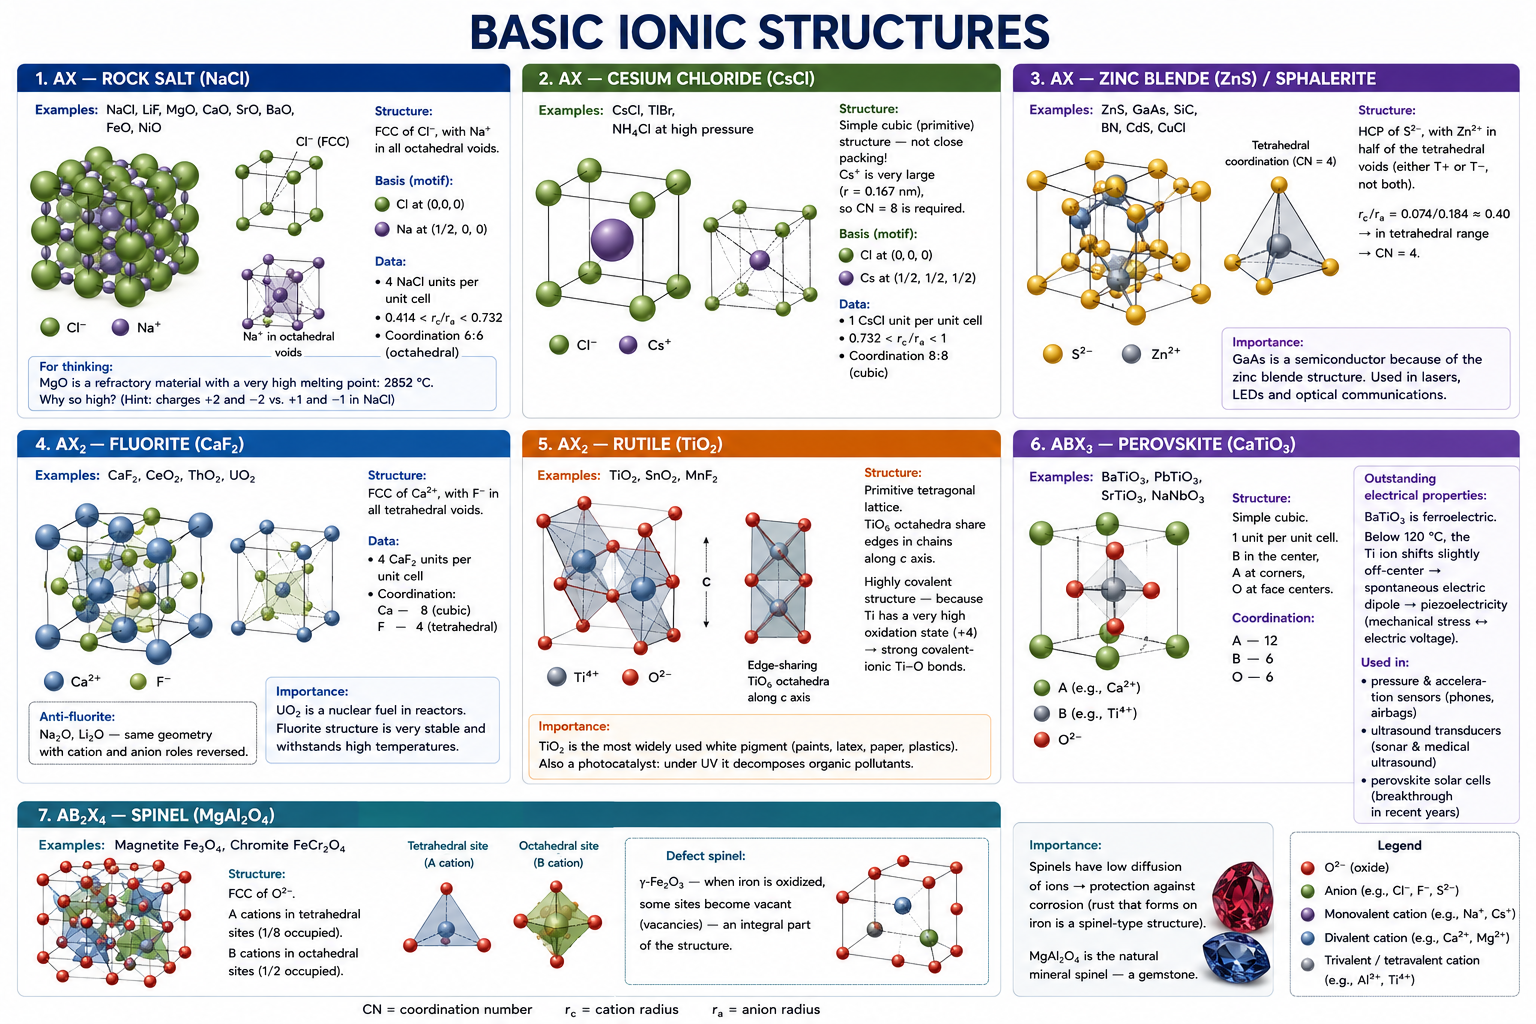
\includegraphics[keepaspectratio]{chapters/../images/image60.ionicStructures.png}}
\#\# 8.6 מבנים קוולנטיים

\subsection{מתי המבנה
קוולנטי?}\label{ux5deux5eaux5d9-ux5d4ux5deux5d1ux5e0ux5d4-ux5e7ux5d5ux5d5ux5dcux5e0ux5d8ux5d9}

כלל האצבע לאופי הקשר לפי דרגת חמצון:

\textbf{מתכות:}

\begin{itemize}
\tightlist
\item
  +1, +2: יוני כמעט תמיד
\item
  +3: גבולי
\item
  +4 ומעלה: \textbf{קוולנטי}
\end{itemize}

\textbf{אל-מתכות:}

\begin{itemize}
\tightlist
\item
  −1, −2: יוני לרוב
\item
  −3: גבולי
\end{itemize}

\textbf{כלל כללי:} כל יסוד בדרגת חמצון \(\geq +4\) → \textbf{קוולנטי},
לא משנה אם מתכת או לא.

\textbf{מתכות מעבר} יכולות להגיע לדרגות חמצון גבוהות (\(+6, +7\)) ---
ולכן מהן נוצרים מבנים קוולנטיים מורכבים.
\pandocbounded{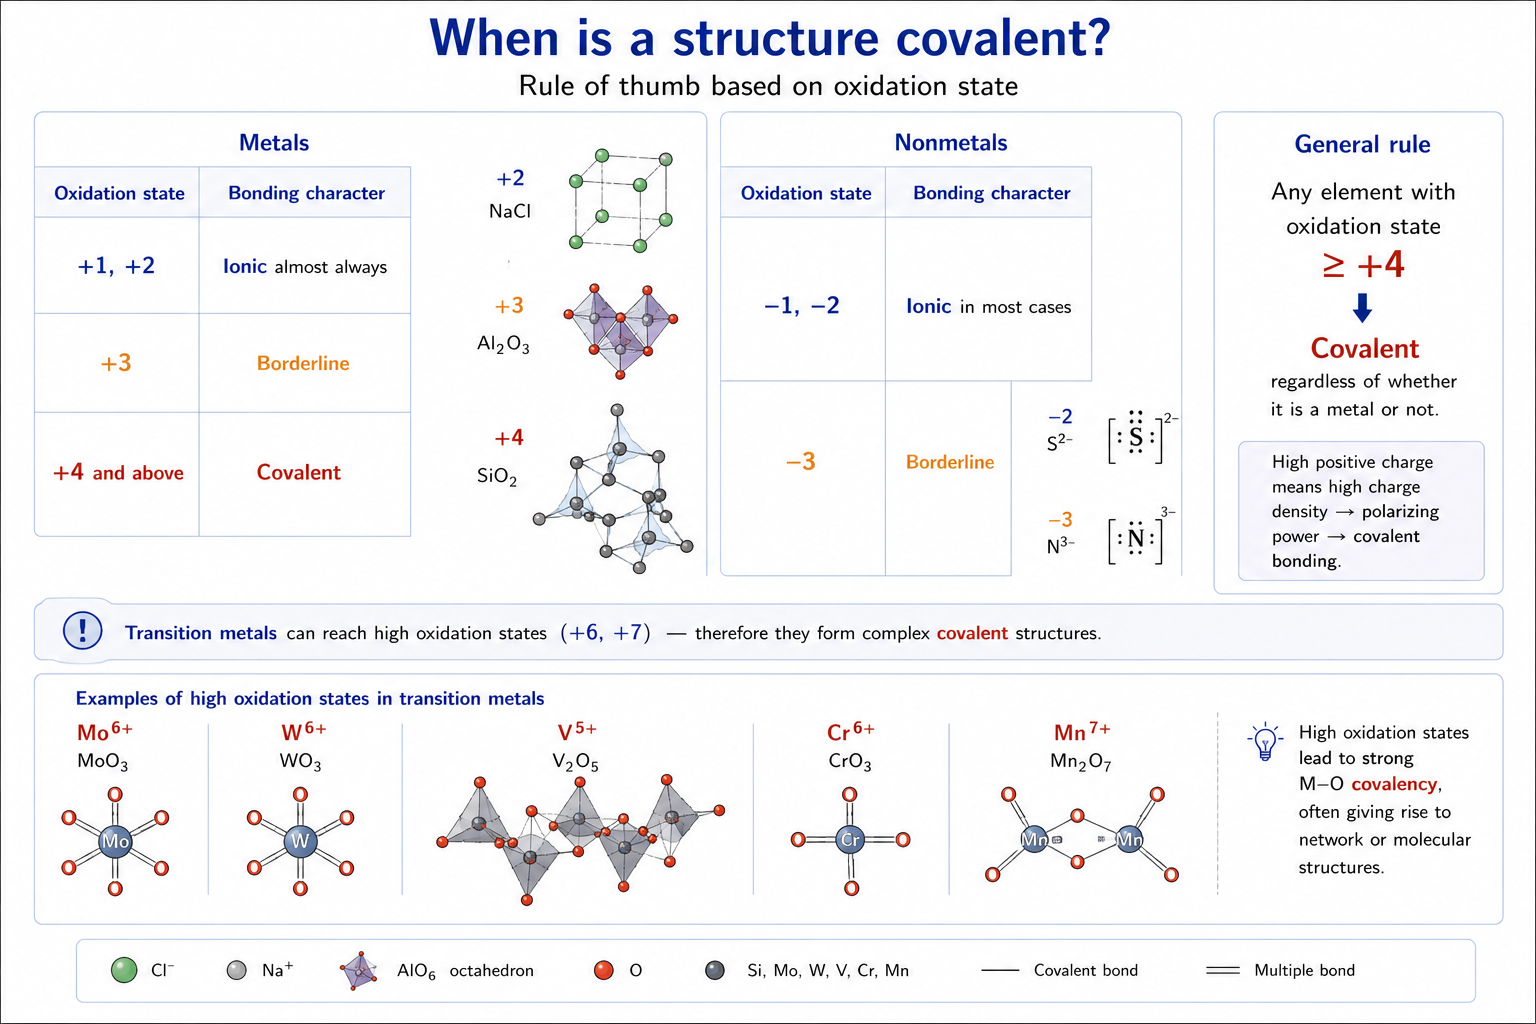
\includegraphics[keepaspectratio]{chapters/../images/image61.whenCovalent.png}}
\#\#\# מבנים של אל-מתכות טהורות

\textbf{יהלום וSiC:} היברידיזציה \(sp^3\), מבנה טטרהדרלי, \(109.5°\). כל
פחמן/סיליקון קשור ל-4 שכנים. \textbf{החומרים הקשים ביותר הידועים}.

\textbf{גרפיט:} היברידיזציה \(sp^2\), שכבות משושות, \(120°\). בין השכבות
--- ון-דר-ולס בלבד (חלש) → גרפיט \textbf{רך ומשמש כסיכה}.

\textbf{גרפן} (graphene) --- שכבה אחת של גרפיט --- הוא המוליך החשמלי
הטוב ביותר הידוע, חזק פי 200 מפלדה, ועוד.

\textbf{גופרית:} היברידיזציה קרובה ל-\(sp^3\), שרשראות ציג-זג → טבעות
\(S_6\), \(S_7\), \(S_8\). המבנה מגוון מאוד --- יש לגופרית למעלה מ-30
אלוטרופים.
\pandocbounded{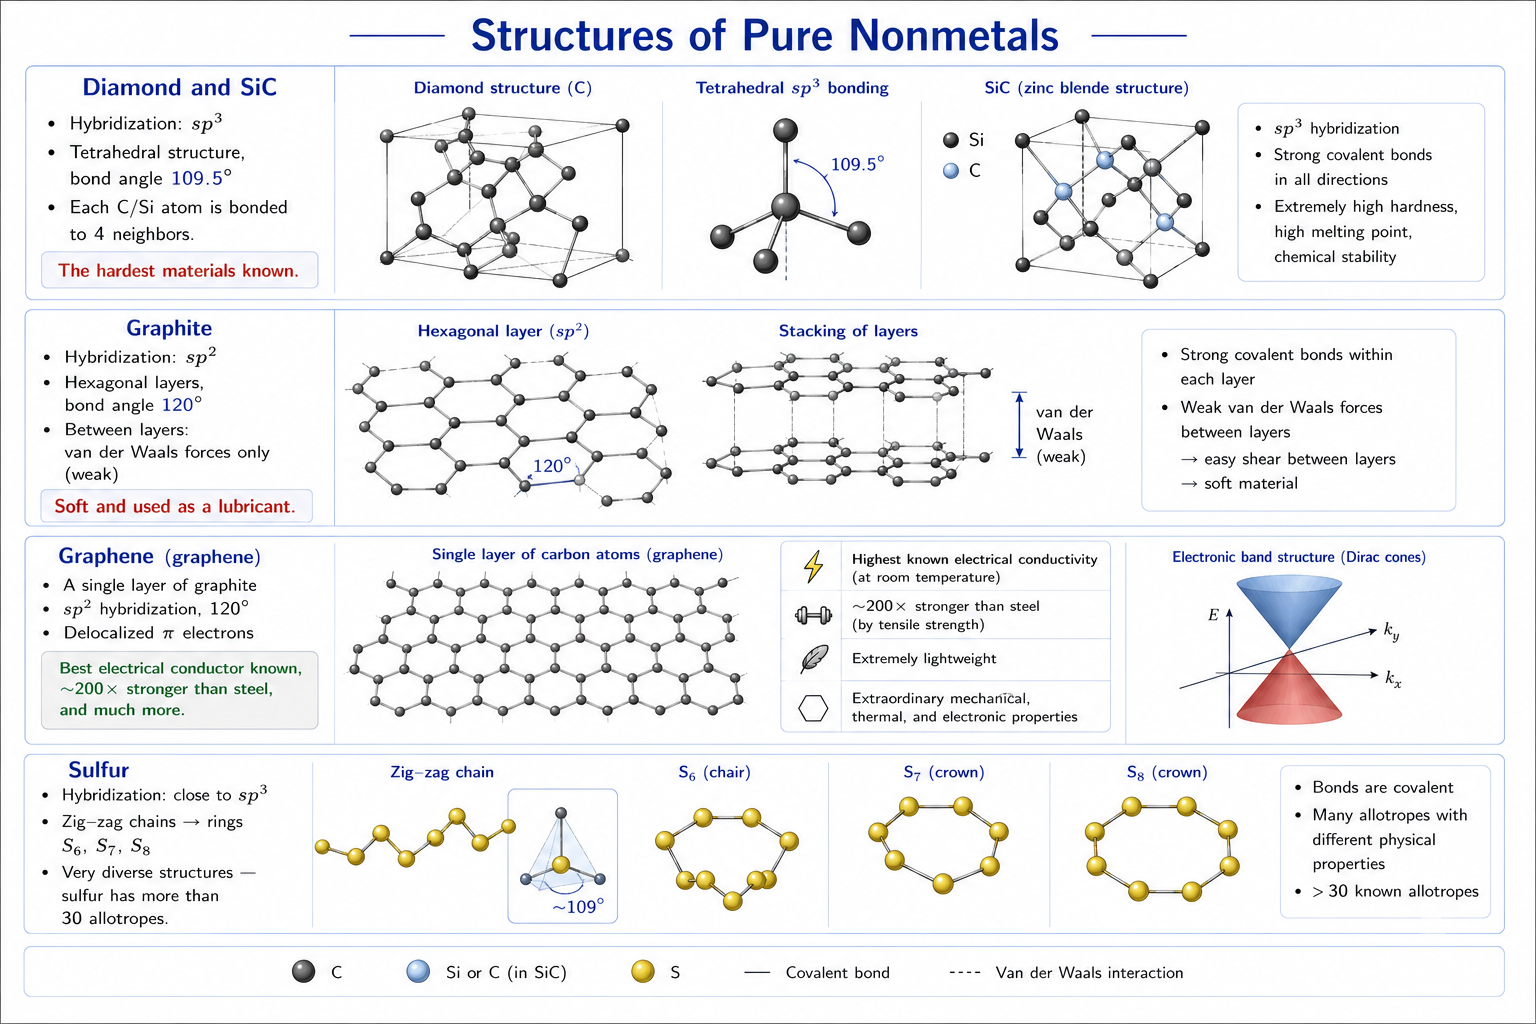
\includegraphics[keepaspectratio]{chapters/../images/image62.PureNonmetals.png}}
\#\#\# חלוקת כל יסודות לפי סוג מבנה
\pandocbounded{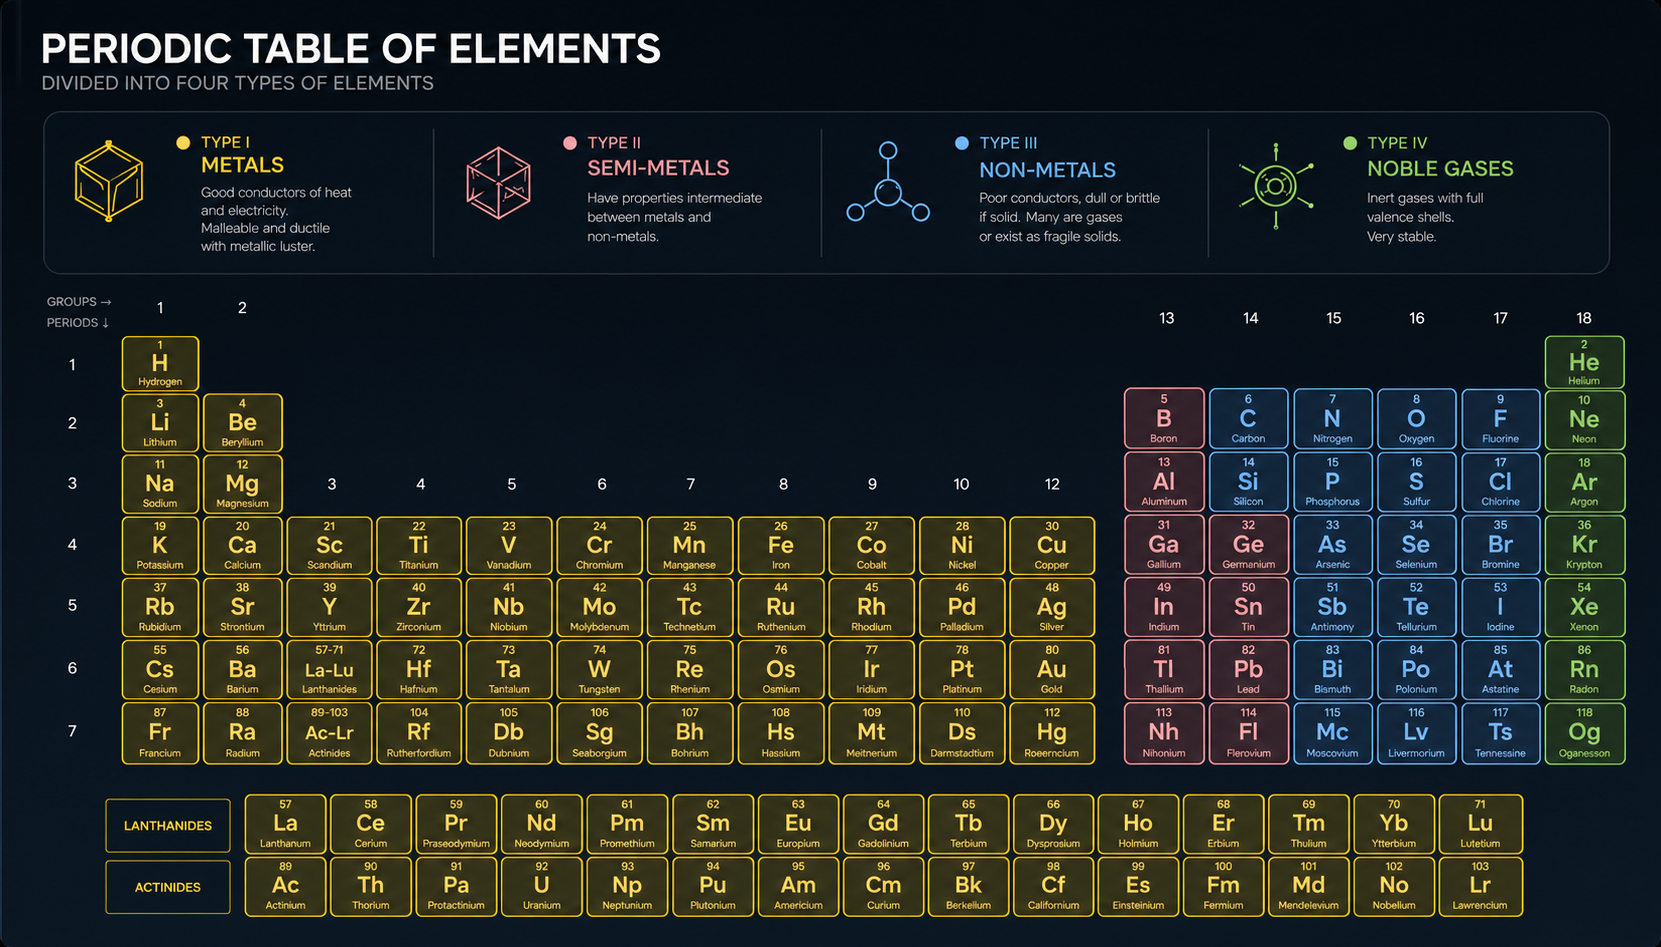
\includegraphics[keepaspectratio]{chapters/../images/image63.TypesOfElements.png}}

\textbf{סוג I --- מתכות:} FCC, HCP, BCC. CN=12 (אריזה צפופה) או CN=8
(BCC). קשרים מתכתיים (אלקטרוני ערכיות חופשיים).

\textbf{סוג II --- מתכות-למחצה} (Si, Ge, Sn, Sb, As\ldots):
\({CN}={8-N}\) כאשר \(N\) מספר הקבוצה. CN נמוך → קשר קוולנטי חלקי.

\textbf{סוג III --- אל-מתכות:} קוולנטיות גבוהה, \({CN}={8-N}\) :

\begin{itemize}
\tightlist
\item
  קב' IV (C, Si): CN=4 → טטרהדרלי
\item
  קב' V (P, As): CN=3 → שכבות
\item
  קב' VI (S, Se, Te): CN=2 → שרשראות
\item
  קב' VII (הלוגנים): CN=1 → מולקולות דו-אטומיות
\end{itemize}

\textbf{סוג IV --- גזים אצילים:} CN=12 --- אריזת FCC/HCP כמו מתכות, אבל
קשר ון-דר-ולס בלבד. מעניין: גז אציל מוצק מתנהג כמו מתכת! \#\# 8.7 חוזק
קשרים ותכונות מוצקים

\subsection{האיזה קשר חזק
יותר?}\label{ux5d4ux5d0ux5d9ux5d6ux5d4-ux5e7ux5e9ux5e8-ux5d7ux5d6ux5e7-ux5d9ux5d5ux5eaux5e8}

שאלה שנראית פשוטה --- אבל התשובה תלויה \textbf{במדד}:

{\def\LTcaptype{none} % do not increment counter
\begin{longtable}[]{@{}llll@{}}
\toprule\noalign{}
מוצק & סוג קשר & אנרגיית סריג (kJ/mol) & \(T_m\) (K) \\
\midrule\noalign{}
\endhead
\bottomrule\noalign{}
\endlastfoot
NaCl & יוני & 779 & 1074 \\
BaO & יוני & 3202 & 2196 \\
יהלום & קוולנטי & 711 & 4470 \\
SiC & קוולנטי & 1183 & 2813 \\
Na & מתכתי & 93 & 371 \\
Cr & מתכתי & 352 & 2150 \\
Ar & ון-דר-ולס & 7.5 & 84 \\
\(\text{H}_2\text{O}\) & מימן & 47 & 273 \\
\end{longtable}
}

\textbf{מסקנה:} לפי אנרגיית סריג, BaO (יוני) חזק מיהלום (קוולנטי). לפי
\(T_m\), יהלום קשיח יותר. \textbf{אין תשובה חד-משמעית} --- תלוי במדד.

\textbf{ברור:} קשרים מתכתיים חלשים יחסית (Cr יוצא דופן), ון-דר-ולס וקשרי
מימן --- חלשים.

\subsection{מדוע מוצקים יוניים
פריכים?}\label{ux5deux5d3ux5d5ux5e2-ux5deux5d5ux5e6ux5e7ux5d9ux5dd-ux5d9ux5d5ux5e0ux5d9ux5d9ux5dd-ux5e4ux5e8ux5d9ux5dbux5d9ux5dd}

כאשר מפעילים כוח גזירה על גביש יוני, שכבות מחליקות. ברגע שהחלקה קורית,
\textbf{יונים עם אותו סימן} מגיעים זה אל מול זה → \textbf{דחייה
אלקטרוסטטית עצומה}.

מחסום האנרגיה לתנועת דיסלוקציות בגביש יוני הוא בלתי-עביר למעשה →
\textbf{שבר פריך}. זו הסיבה שקרמיקה מתנפצת ולא מתעקלת.

מתכות, לעומת זאת, גמישות --- כי אלקטרוני הערכיות החופשיים ``עוטפים'' את
היונים המוזזים ומונעים דחייה גדולה. \#\# חלק ג': תורת שדה הגביש --- CFT
\#\# 8.8 מתכות מעבר ואורביטלי d

\subsection{מדוע מתכות מעבר
מיוחדות?}\label{ux5deux5d3ux5d5ux5e2-ux5deux5eaux5dbux5d5ux5ea-ux5deux5e2ux5d1ux5e8-ux5deux5d9ux5d5ux5d7ux5d3ux5d5ux5ea}

מתכות מעבר (Sc עד Zn בשורה 4, ועוד) בעלות \textbf{אורביטלי d} מלאים
חלקית בלבד. האורביטלים הללו:

\begin{itemize}
\tightlist
\item
  יוצרים קשרים קוולנטיים בדרגות חמצון גבוהות
\item
  גורמים לצבעים עזים (Cu כחול, Cr ירוק, Fe חלוד-אדום)
\item
  יוצרים מגנטיות
\item
  מגיבים לסביבה הקרובה --- וכאן נכנסת תורת שדה הגביש
\end{itemize}

\subsection{שחזור: חמשת אורביטלי
d}\label{ux5e9ux5d7ux5d6ux5d5ux5e8-ux5d7ux5deux5e9ux5ea-ux5d0ux5d5ux5e8ux5d1ux5d9ux5d8ux5dcux5d9-d}

מפתרון משוואת שרדינגר עבור \(l=2\), מקבלים 5 אורביטלים:

\begin{itemize}
\tightlist
\item
  \(d_{xy}\), \(d_{xz}\), \(d_{yz}\): ``ממוקמים בין'' הצירים, לובשים
  צורת ארבע אונות בין ה-x,y,z
\item
  \(d_{x^2-y^2}\): ממוקם \textbf{על} הצירים x, y
\item
  \(d_{z^2}\): ממוקם \textbf{על} ציר z (עם ``חגורה'' ב-xy)
\end{itemize}

\textbf{באטום מבודד:} כל חמשת האורביטלים \textbf{מנוונים} --- אנרגיות
שוות לחלוטין.
\pandocbounded{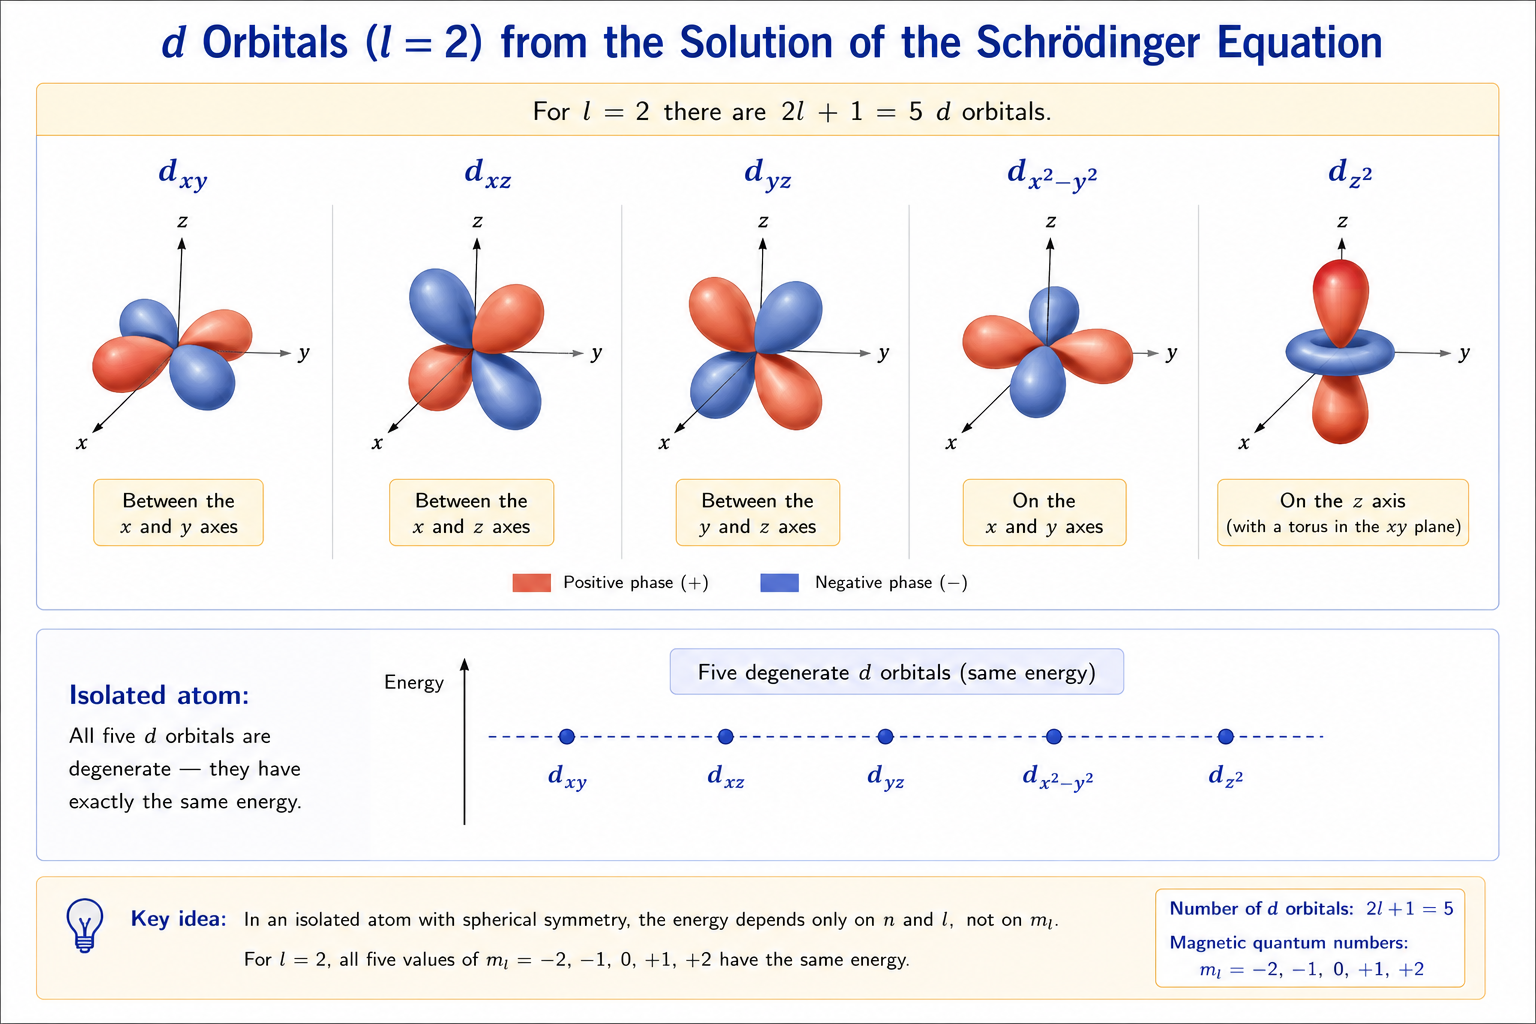
\includegraphics[keepaspectratio]{chapters/../images/image64.d-orbitals.png}}
\#\# 8.9 פיצול בשדה אוקטהדרלי

\subsection{הרעיון
המרכזי}\label{ux5d4ux5e8ux5e2ux5d9ux5d5ux5df-ux5d4ux5deux5e8ux5dbux5d6ux5d9-1}

\textbf{תורת שדה הגביש} (Crystal Field Theory, CFT; בת'ה ו-ון-וולק,
1929--1932) מתארת אטום מרכזי מוקף בששה ליגנדים (שכנים) שנחשבים
\textbf{מטענים נקודתיים} שליליים.

כאשר ששת הליגנדים מתקרבים מכל ששת הכיוונים (\(\pm x\), \(\pm y\),
\(\pm z\)), הם יוצרים שדה חשמלי שמשפיע באופן \textbf{שונה} על חמשת
אורביטלי d:

\textbf{\(d_{x^2-y^2}\) ו-\(d_{z^2}\)} --- מכוונים \textbf{ישירות} לעבר
הליגנדים → נדחים חזק → \textbf{אנרגיה גבוהה} → נקראים \textbf{\(e_g\)}

\textbf{\(d_{xy}\), \(d_{xz}\), \(d_{yz}\)} --- עוברים \textbf{בין}
הצירים → רחוקים יחסית מהליגנדים → נדחים פחות → \textbf{אנרגיה נמוכה} →
נקראים \textbf{\(t_{2g}\)}

\textbf{התוצאה:} חמשת האורביטלים המנוונים \textbf{מתפצלים לשתי
תת-קבוצות}:

\[E(e_g) = E_\text{בסיס} + \frac{3}{5}\Delta_O\]

\[E(t_{2g}) = E_\text{בסיס} - \frac{2}{5}\Delta_O\]

כאשר \(\Delta_O\) (או \(\Delta_o\)) נקרא \textbf{אנרגיית פיצול שדה
הגביש}.

\textbf{שימו לב:}
\(\frac{3}{5} \times 2 + \frac{2}{5} \times 3 = \frac{6}{5} + \frac{6}{5}\)\ldots{}
לא מדויק. הסכום הנכון:
\(2 \times \frac{3}{5}\Delta - 3 \times \frac{2}{5}\Delta = 0\) ---
הממוצע נשמר, רק חלוקה מחדש.
\pandocbounded{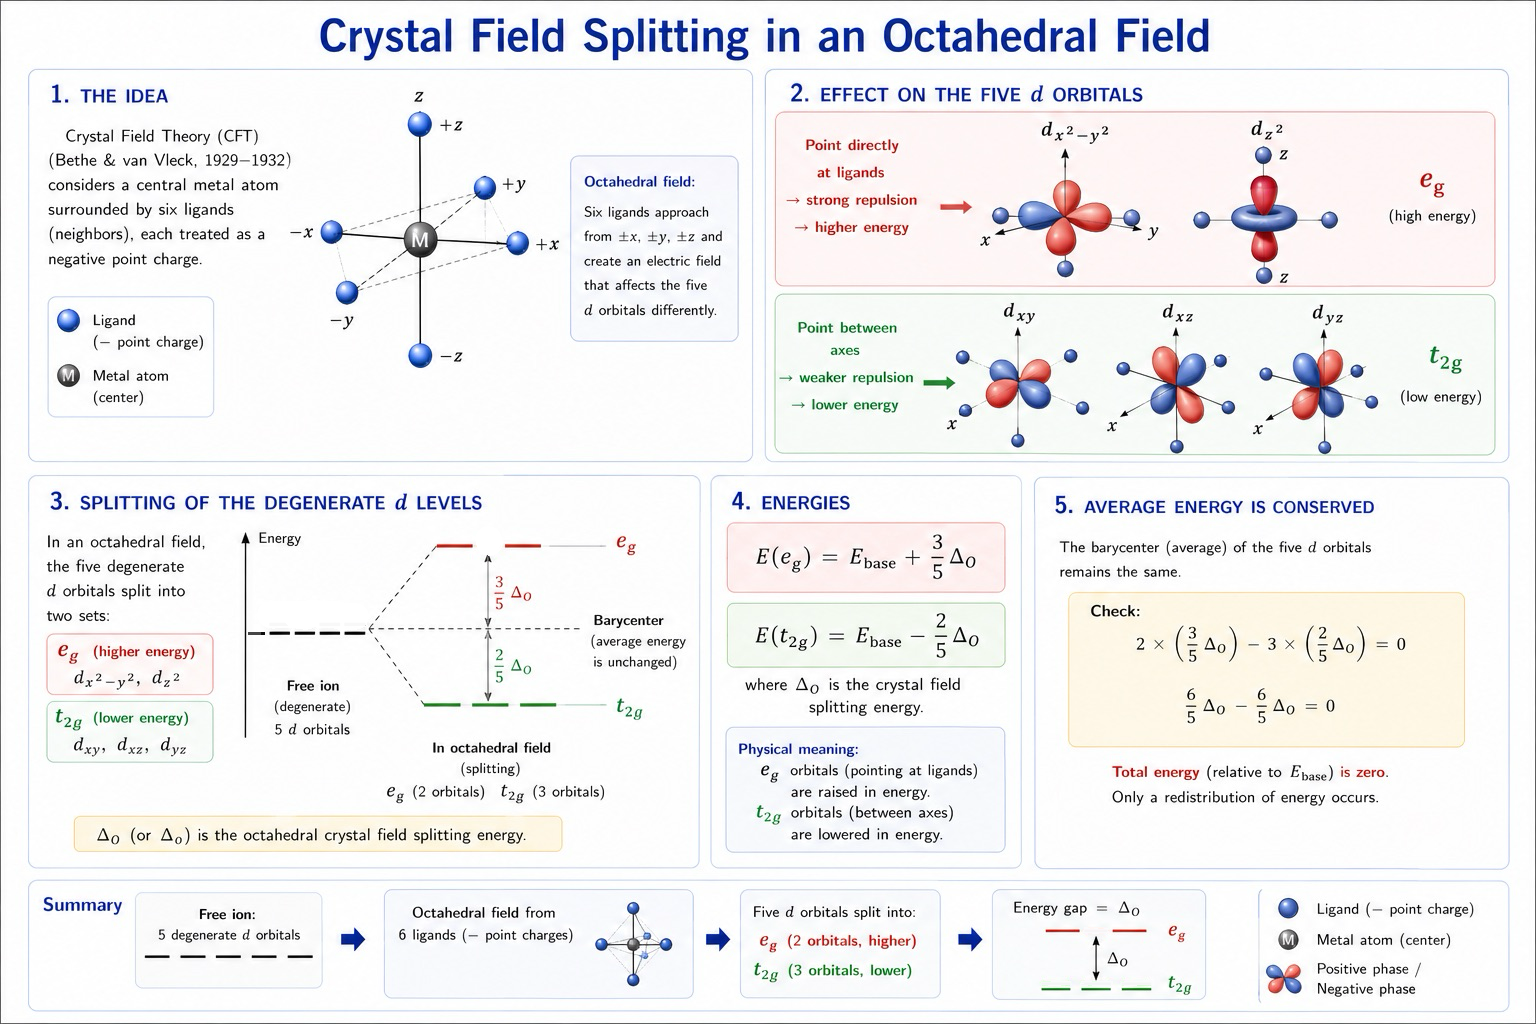
\includegraphics[keepaspectratio]{chapters/../images/image65.octahedralSplitting.png}}
\#\# 8.10 סדרת שדה הליגנד

\subsection{\texorpdfstring{מה קובע את
\(\Delta\)?}{מה קובע את \textbackslash Delta?}}\label{ux5deux5d4-ux5e7ux5d5ux5d1ux5e2-ux5d0ux5ea-delta}

ליגנדים שונים מפצלים בחוזק שונה. \textbf{הסדרה הספקטרוכימית} (אמפירית):

\[I^- < Br^- < S^{2-} < Cl^- < F^- < OH^- < H_2O < NH_3 < NO_2^- < CN^- < CO\]

\textbf{ליגנדים חלשים} (שמאל) --- \(\Delta\) קטן. \textbf{ליגנדים חזקים}
(ימין) --- \(\Delta\) גדול.

\textbf{מדוע?} ליגנדים חזקים הם \textbf{תורמי π} --- יש להם זוגות
אלקטרונים לא-קושרים שהם יכולים לתרום לאורביטלי d של המתכת בקשר π, מה
שמגדיל את הפיצול. ליגנדים חלשים הם \textbf{מקבלי π} --- ``שואבים''
צפיפות אלקטרונים מהמתכת ומקטינים את הפיצול.

\textbf{\(CN^-\) ו-\(CO\)} הם הליגנדים החזקים ביותר --- בשל קשר π חזק
מאוד. לכן מולקולת CO רעילה: היא קושרת חזק ל-\(\text{Fe}^{2+}\)
בהמוגלובין (\(CN^-\) גם כן רעיל מאותה סיבה). \#\# 8.11 אנרגיית ייצוב שדה
גביש (CFSE)

\subsection{חישוב}\label{ux5d7ux5d9ux5e9ux5d5ux5d1}

האלקטרונים ממלאים את אורביטלי \(t_{2g}\) (אנרגיה נמוכה) לפני \(e_g\)
(אנרגיה גבוהה). ה\textbf{רווח האנרגטי} נקרא \textbf{CFSE}:

\[\text{CFSE} = \Delta_O \left(\frac{2}{5} N_{t_{2g}} - \frac{3}{5} N_{e_g}\right)\]

\textbf{דוגמה --- \(\text{Ti}^{3+}\) (\(d^1\)):} אלקטרון אחד
ב-\(t_{2g}\):
\[\text{CFSE} = \Delta_O \left(\frac{2}{5} \cdot 1 - 0\right) = \frac{2}{5}\Delta_O\]

\textbf{דוגמה --- \(\text{Fe}^{3+}\) ספין-גבוה (\(d^5\)):} כל חמשת
האורביטלים עם אלקטרון אחד:
\[\text{CFSE} = \Delta_O\left(\frac{2}{5} \cdot 3 - \frac{3}{5} \cdot 2\right) = 0\]

ולכן \(\text{Fe}^{3+}\) בליגנדים חלשים (כמו מים) \textbf{כמעט חסר CFSE}
--- ולכן קל יחסית לחמצן/לצמצם. \#\# 8.12 ספין גבוה וספין נמוך

\subsection{התחרות}\label{ux5d4ux5eaux5d7ux5e8ux5d5ux5ea}

עבור \(d^4\)--\(d^7\), קיימות שתי אפשרויות:

\textbf{ספין גבוה (high-spin):} מעדיפים לפזר על כל 5 האורביטלים (כלל
הונד) → יותר אלקטרונים בלתי-מזווגים.

\textbf{ספין נמוך (low-spin):} מעדיפים למלא \(t_{2g}\) לפני מעבר
ל-\(e_g\) → פחות אלקטרונים בלתי-מזווגים.

\textbf{מה קובע?} תחרות בין שתי אנרגיות:

\begin{itemize}
\tightlist
\item
  \(\Delta_O\) --- כמה ``שווה'' להישאר ב-\(t_{2g}\)
\item
  \(P\) --- אנרגיית הזיווג (כמה עולה לשים שני אלקטרונים באותו אורביטל)
\end{itemize}

{\def\LTcaptype{none} % do not increment counter
\begin{longtable}[]{@{}ll@{}}
\toprule\noalign{}
תנאי & תוצאה \\
\midrule\noalign{}
\endhead
\bottomrule\noalign{}
\endlastfoot
\(\Delta_O > P\) (ליגנדים חזקים) & ספין נמוך \\
\(\Delta_O < P\) (ליגנדים חלשים) & ספין גבוה \\
\end{longtable}
}

\subsection{תוצאות}\label{ux5eaux5d5ux5e6ux5d0ux5d5ux5ea}

\textbf{מגנטיות:}

\begin{itemize}
\tightlist
\item
  \textbf{ספין נמוך:} כל אלקטרונים מזווגים → \textbf{דיאמגנטי} (נדחה מ
  שדה מגנטי)
\item
  \textbf{ספין גבוה:} אלקטרונים בלתי-מזווגים → \textbf{פרמגנטי} (נמשך
  לשדה מגנטי)
\end{itemize}

\textbf{צבע:} ספין גבוה → \(\Delta_O\) קטן → פוטון בעל אנרגיה נמוכה →
ספיגה בטווח ארוך-גל (אדום) → הצבע הנראה כחול-ירוק.
\pandocbounded{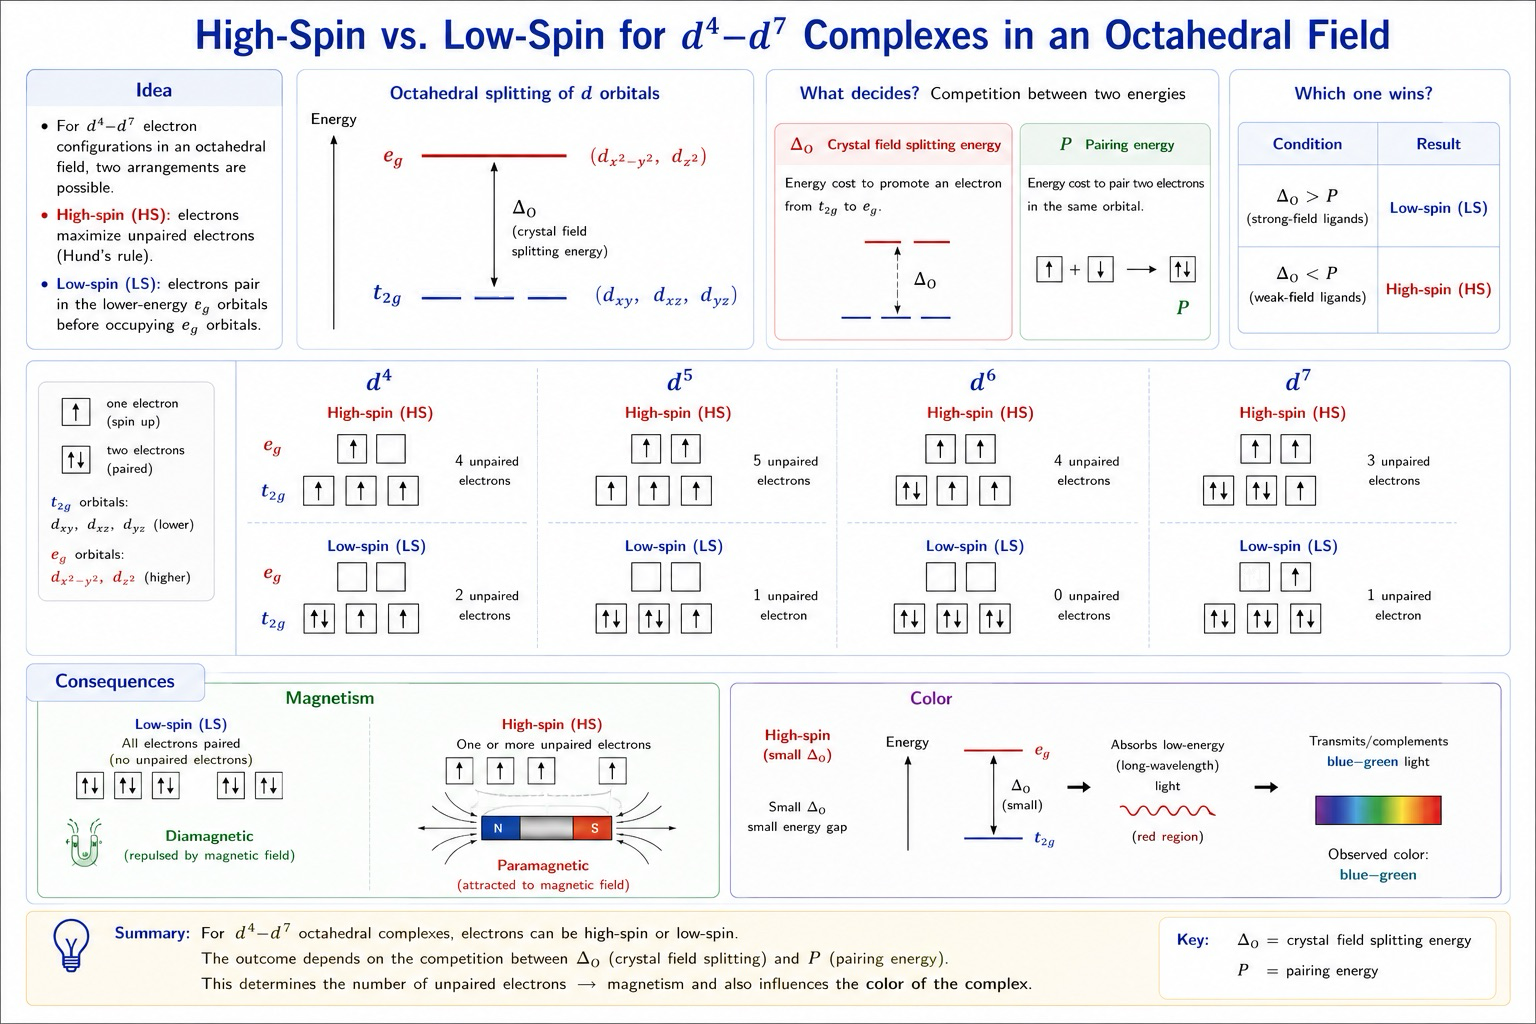
\includegraphics[keepaspectratio]{chapters/../images/image66.HS_LS.png}}
\#\# 8.13 צבע במתכות מעבר

\subsection{העקרון}\label{ux5d4ux5e2ux5e7ux5e8ux5d5ux5df}

כאשר פוטון בעל אנרגיה \(\Delta E = \Delta_O\) פוגע במולקולה, הוא
\textbf{נספג} --- אלקטרון עולה מ-\(t_{2g}\) ל-\(e_g\). הצבע
\textbf{הנראה} הוא \textbf{הצבע המשלים} לצבע שנספג.

\textbf{גלגל הצבעים:} ירוק ↔ אדום; כחול ↔ כתום; צהוב ↔ סגול.

\textbf{דוגמה --- חישוב:}

קומפלקס טטרהדרלי (שדה \(\Delta_t \approx \frac{4}{9}\Delta_O\)) סופג
ב-\(\lambda = 545\ \text{nm}\). מהו \(\Delta_O\)?

\[\Delta_t = \frac{hc}{\lambda} = \frac{(6.626 \times 10^{-34})(3 \times 10^8)}{545 \times 10^{-9}} = 3.65 \times 10^{-19}\ \text{J} = 2.3\ \text{eV}\]

\[\Delta_O = \frac{\Delta_t}{4/9} = \frac{9}{4} \times 3.65 \times 10^{-19} = 8.21 \times 10^{-19}\ \text{J} = 5.1\ \text{eV}\]

הקומפלקס סופג ירוק (\(545\ \text{nm}\)) → \textbf{צבע נראה: סגול-אדום}.

\textbf{דוגמאות מחיי יומיום:}

{\def\LTcaptype{none} % do not increment counter
\begin{longtable}[]{@{}lll@{}}
\toprule\noalign{}
יון & ליגנד & צבע \\
\midrule\noalign{}
\endhead
\bottomrule\noalign{}
\endlastfoot
\(\text{Cu}^{2+}\) & \(\text{H}_2\text{O}\) & כחול (מים כחולים!) \\
\(\text{Cr}^{3+}\) & \(\text{H}_2\text{O}\) & ירוק (כרום ירוק) \\
\(\text{Fe}^{3+}\) & \(\text{H}_2\text{O}\) & צהוב-חום (חלודה) \\
\(\text{Co}^{2+}\) & \(\text{Cl}^-\) & כחול \\
\(\text{Co}^{2+}\) & \(\text{H}_2\text{O}\) & ורוד \\
\end{longtable}
}

\section{חלק ד': מעברים
פולימורפיים}\label{ux5d7ux5dcux5e7-ux5d3-ux5deux5e2ux5d1ux5e8ux5d9ux5dd-ux5e4ux5d5ux5dcux5d9ux5deux5d5ux5e8ux5e4ux5d9ux5d9ux5dd}

\section{8.14 תגובות בפאזה
מוצקה}\label{ux5eaux5d2ux5d5ux5d1ux5d5ux5ea-ux5d1ux5e4ux5d0ux5d6ux5d4-ux5deux5d5ux5e6ux5e7ux5d4}

\subsection{מדוע
איטיות?}\label{ux5deux5d3ux5d5ux5e2-ux5d0ux5d9ux5d8ux5d9ux5d5ux5ea}

\textbf{דיפוזיה} --- תנועת אטומים או יונים בתוך מוצק --- \textbf{איטית
מאוד}:

\[D_\text{solid} \sim 10^{-11}\ \text{cm}^2/\text{s}\]
\[D_\text{liquid} \sim 10^{-5}\ \text{cm}^2/\text{s}\]
\[D_\text{gas} \sim 1\ \text{cm}^2/\text{s}\]

נוזל מהיר פי \(10^6\) ממוצק; גז --- פי \(10^{11}\). לכן תגובות בפאזה
מוצקה מתרחשות לרוב רק מעל \(\sim 0.5,T_m\).

\textbf{השלכה:} ייצור קרמיקה (SiC, \(\text{Al}_2\text{O}_3\)\ldots) דורש
חימום ממושך בטמפרטורות גבוהות מאוד --- כדי לאפשר דיפוזיה מספקת לצורך
ריאקציה מלאה.

\textbf{מעברים פולימורפיים} --- כאשר \textbf{אותו חומר} משנה את הפאזה
הגבישית שלו (שינוי מבנה, לא הרכב). \#\# 8.15 תרמודינמיקה: כלל הפאזות של
גיבס

\subsection{הכלל}\label{ux5d4ux5dbux5dcux5dc-1}

\[P + F = C + \text{Param}\]

\begin{itemize}
\tightlist
\item
  \(P\) --- מספר פאזות קיימות
\item
  \(F\) --- דרגות חופש (כמה משתנים אינטנסיביים אפשר לשנות עצמאית)
\item
  \(C\) --- מספר רכיבים כימיים
\item
  \(\text{Param}\) --- מספר המשתנים (בדרך כלל 2: \(T\) ו-\(P\))
\end{itemize}

\textbf{עבור מערכת חד-רכיבית} (\(C=1\)) כמו מים: מקסימום פאזות כאשר
\(F=0\): \[P_\text{max} = 1 + 2 = 3\]

לכן מים יכולים להיות בשלוש פאזות בו-זמנית --- \textbf{נקודה משולשת}
(triple point) ב-\(0.006\ \text{atm}\), \(273.16\ \text{K}\).

\subsection{מטא-יציבות}\label{ux5deux5d8ux5d0-ux5d9ux5e6ux5d9ux5d1ux5d5ux5ea}

\textbf{מדוע יכולות להתקיים יותר מפאזה אחת בתנאים נתונים?}

כל פאזה מתאימה ל\textbf{בור פוטנציאל} שונה. הבור \textbf{העמוק ביותר} =
\textbf{פאזה יציבה}; בורות רדודים יותר = \textbf{פאזות מטא-יציבות}.

כדי לעבור מפאזה מטא-יציבה ליציבה, צריך \textbf{לטפס מחסום} --- לעבור דרך
מצב ביניים בעל אנרגיה \textbf{גבוהה יותר} מהפאזה הנוכחית (שיא
הפוטנציאל).

\textbf{דוגמה:} יהלום הוא \textbf{מטא-יציב} בתנאים רגילים --- גרפיט יציב
יותר. אבל המחסום כל כך גבוה שיהלום ``ישן'' לנצח בלי להיות גרפיט. ניסוי
מחשבתי: עם מספיק אנרגיה (חום עצום) --- יהלום יהפוך לגרפיט. \#\# 8.16
סוגי מעברים פולימורפיים

\subsection{מסדר ראשון מול
שני}\label{ux5deux5e1ux5d3ux5e8-ux5e8ux5d0ux5e9ux5d5ux5df-ux5deux5d5ux5dc-ux5e9ux5e0ux5d9}

\textbf{מעבר מסדר ראשון} --- יש \textbf{חום סמוי} (latent heat): המערכת
סופגת/משחררת אנרגיה בטמפרטורה קבועה, בעוד שתי פאזות מתקיימות יחד.

\begin{itemize}
\tightlist
\item
  דוגמאות: המסת קרח, רתיחת מים, כל התכות מתכת
\item
  נגזרות ראשונות של הפוטנציאל (נפח, אנטרופיה) \textbf{קופצות}
\end{itemize}

\textbf{מעבר מסדר שני} --- \textbf{אין} חום סמוי; הסימטריה משתנה בהדרגה.

\begin{itemize}
\tightlist
\item
  דוגמאות: מעבר פרומגנטי (נקודת קיורי), מעבר על-מוליך, מעבר על-זורם
\item
  נגזרות שניות (קיבולת חום, דחיסות) \textbf{קופצות}
\end{itemize}

\subsection{מעברים בינוי-מחדש
(Reconstructive)}\label{ux5deux5e2ux5d1ux5e8ux5d9ux5dd-ux5d1ux5d9ux5e0ux5d5ux5d9-ux5deux5d7ux5d3ux5e9-reconstructive}

\textbf{מאפיין:} קשרים קיימים \textbf{נשברים} ונוצרים קשרים חדשים.

\textbf{תוצאה:} מחסום \textbf{גבוה מאוד} → מהירות \textbf{נמוכה מאוד}.

\textbf{דוגמאות:}

\begin{itemize}
\tightlist
\item
  \textbf{יהלום ↔ גרפיט}: קשרי \(sp^3\) ↔ \(sp^2\). בתנאים רגילים, המעבר
  גרפיט→יהלום דורש לחץ של \(\sim 50\ \text{kbar}\) בנוכחות מתכת-מאיץ
  ב-\(\sim 1500°C\) --- כך מייצרים יהלומים סינתטיים.
\item
  \textbf{בדיל לבן ↔ בדיל אפור}: מתחת ל-\(13°C\), בדיל לבן (מבנה מתכתי)
  אמור להפוך לאפור (מבנה \(sp^3\) כמו יהלום). המעבר איטי מאוד --- אבל
  בחורף קנדי קיצוני, כפתורי בדיל על מעילי חיילים הנפולאוניים אכן
  התפוררו. \textbf{``מגפת הבדיל''}.
\end{itemize}

\subsection{מעברים ללא-דיפוזיה
(Displacive)}\label{ux5deux5e2ux5d1ux5e8ux5d9ux5dd-ux5dcux5dcux5d0-ux5d3ux5d9ux5e4ux5d5ux5d6ux5d9ux5d4-displacive}

\textbf{מאפיין:} \textbf{ללא} שבירת קשרים --- רק \textbf{הזזות קטנות} של
אטומים ממיקומם. מחסום \textbf{קטן} → מהיר יחסית.

\textbf{דוגמה:} גרפיט תחת לחץ מתעוות לביניים משושה ואז ליהלום --- רק
שינוי זווית מ-\(120°\) ל-\(109.5°\), ללא שבירת קשרים.

\subsection{מעברים מרטנסיטיים
(Martensitic)}\label{ux5deux5e2ux5d1ux5e8ux5d9ux5dd-ux5deux5e8ux5d8ux5e0ux5e1ux5d9ux5d8ux5d9ux5d9ux5dd-martensitic}

\textbf{מאפיין:} מקרה קיצוני של displacive --- \textbf{מיידי}. גל מבנה
עובר בחומר במהירות קול.

\textbf{דוגמה הכי חשובה:} \textbf{פלדה}.

\textbf{ברזל} (Fe) עובר מעברים מרכזיים:

\begin{itemize}
\tightlist
\item
  מתחת ל-\(912°C\): \(\alpha\)-Fe (BCC, פרמגנטי) = \textbf{פריט}
  (ferrite)
\item
  \(912°C\)--\(1394°C\): \(\gamma\)-Fe (FCC) = \textbf{אוסטניט}
  (austenite)
\item
  מעל \(1394°C\) עד היתוך: \(\delta\)-Fe (BCC)
\end{itemize}

\textbf{פלדה} = ברזל + 0.02\%--2\% פחמן. בחימום, פחמן מתמוסס
ב-\(\gamma\)-Fe (FCC) עד 2.1\%. בצינון מהיר (\textbf{כיבוי} ---
quenching), ה-FCC הופך ל-BCC מרטנזיטי בטמפרטורה נמוכה כשאין זמן לפחמן
לצאת → \textbf{מרטנזיט} = BCC מעוות עם פחמן לכוד. \textbf{קשה מאוד
ופריך}.

בצינון איטי → פריט + ציט (Fe₃C) = \textbf{פרליט} = רך יותר אבל גמיש.

\textbf{כך נקבעות תכונות פלדה} --- על ידי בקרת קצב הצינון!

\subsection{מעברי
סדר-אי-סדר}\label{ux5deux5e2ux5d1ux5e8ux5d9-ux5e1ux5d3ux5e8-ux5d0ux5d9-ux5e1ux5d3ux5e8}

\textbf{מאפיין:} \textbf{הסדר} של המערכת משתנה --- לא המבנה הכימי.

\textbf{דוגמאות:}

\begin{itemize}
\tightlist
\item
  \textbf{מעבר פרומגנטי} (נקודת קיורי): מתחת ל-\(T_C\), ספינים מיושרים →
  מגנט. מעל \(T_C\) --- ספינים אקראיים. עבור ברזל: \(T_C = 770°C\).
\item
  \textbf{על-מוליכות}: מתחת ל-\(T_c\) --- עמידות אפסית. מעל --- עמידות
  רגילה.
\item
  \textbf{סגסוגות מסודרות}: ב-\(\text{CuZn}\) (פליז) --- מתחת לטמפרטורה
  מסוימת Cu ו-Zn מסודרים לחלופין; מעל --- אקראי.
\end{itemize}

\textbf{כלל:} \textbf{ככל שהטמפרטורה גבוהה יותר, כך הפאזה עם הסימטריה
הגבוהה יותר יציבה.} מצב אקראי לחלוטין = סימטריה ספירית = גבוהה ביותר.
\pandocbounded{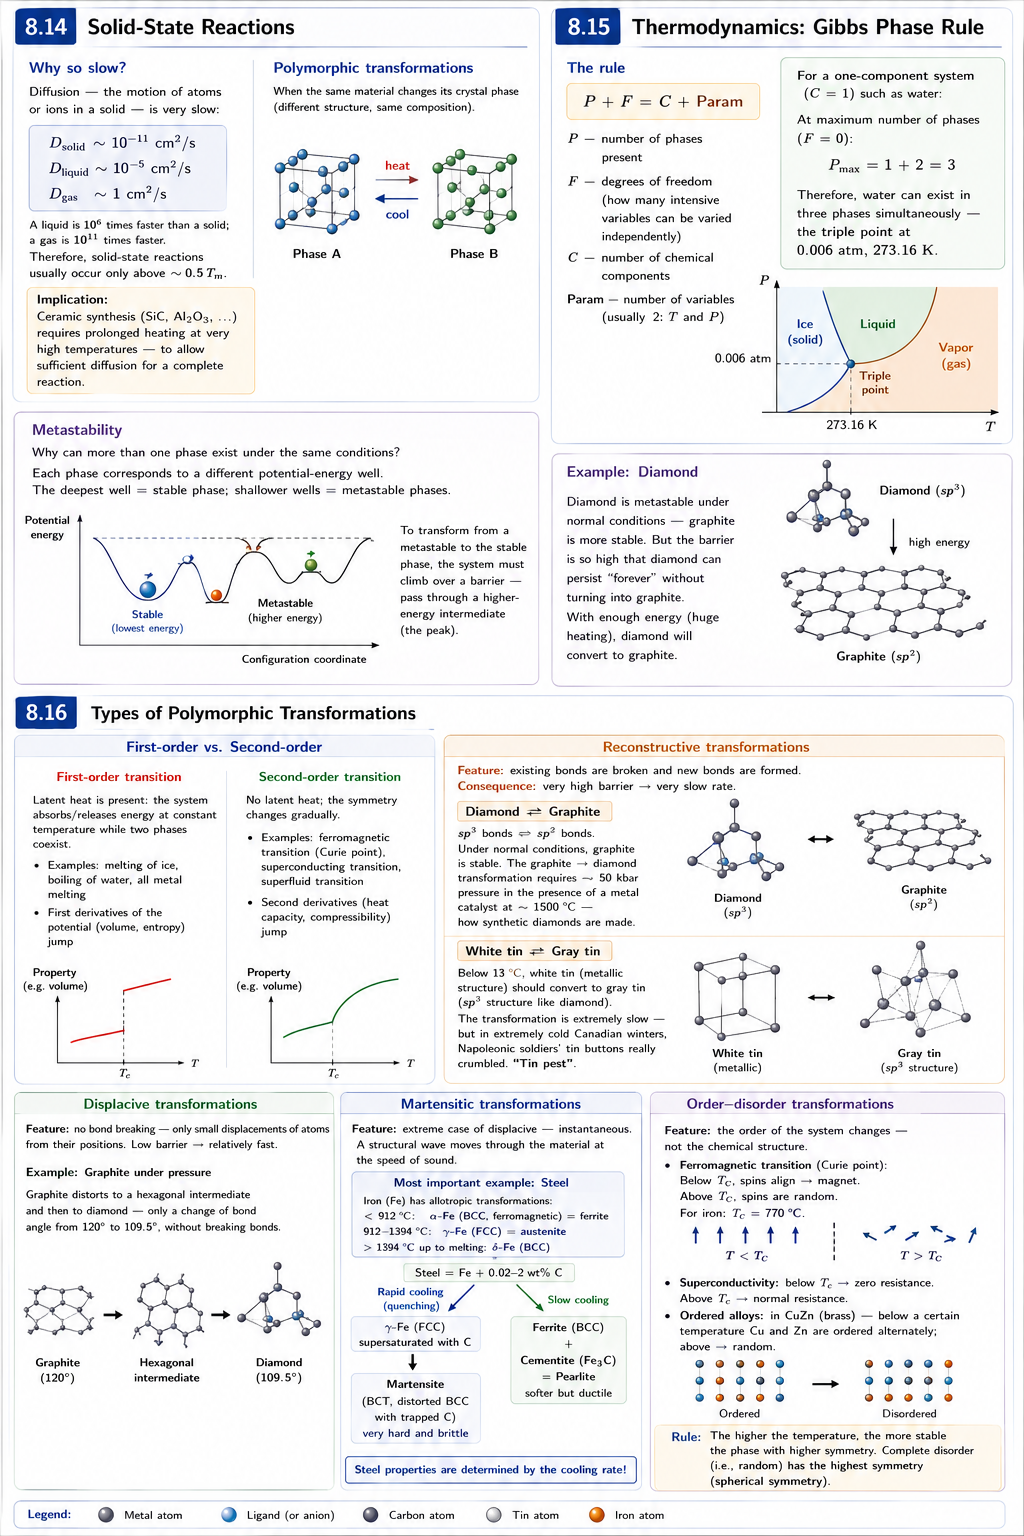
\includegraphics[keepaspectratio]{chapters/../images/image67.polymorphism.png}}
\#\# סיכום

{\def\LTcaptype{none} % do not increment counter
\begin{longtable}[]{@{}
  >{\raggedright\arraybackslash}p{(\linewidth - 2\tabcolsep) * \real{0.1786}}
  >{\raggedright\arraybackslash}p{(\linewidth - 2\tabcolsep) * \real{0.8214}}@{}}
\toprule\noalign{}
\begin{minipage}[b]{\linewidth}\raggedright
נושא
\end{minipage} & \begin{minipage}[b]{\linewidth}\raggedright
מה ראינו
\end{minipage} \\
\midrule\noalign{}
\endhead
\bottomrule\noalign{}
\endlastfoot
אריזות & FCC/HCP --- \(74%
\) אריזה. 2T + 1O וואידים לאטום \\
מבנים יוניים & חוקי פולינג. NaCl, CsCl, ZnS, פלואוריט, פרובסקיט,
ספינל \\
מבנים קוולנטיים & כיוון הקשרים קובע מבנה. יהלום/גרפיט/גופרית \\
CFT & פיצול d לעג/t2g. \(\Delta_O\) תלוי בליגנד. ספין גבוה/נמוך \\
צבע & הצבע הנספג = \(\Delta_O\); הצבע הנראה = משלים \\
מעברים & בינוי-מחדש (איטי) / displacive (מהיר) / מרטנזיטי (מיידי) /
סדר-אי-סדר \\
\end{longtable}
}




\end{document}
